\chapter{Le scuole di Magia}

\newcommand{\Simbolo}[1] {\begin{center}\includegraphics{#1}\end{center}}

\section{Le scuole di magia}
\label{scuole}

Con il termine ``Scuola di Magia'' si indica
la codificazione di regole e insegnamenti indirizzati verso
determinati tipi di incantesimi (a seconda della categoria funzionale
favorita dalla scuola, vedi paragrafo seguente). Le scuole indicano a
grandi linee la branca della magia praticata dai suoi adepti.

Le caratteristiche di ciascuna
scuola sono:

\begin{description}
  
\item{\bf Dominio.} Il Dominio di una Scuola \`e la parte di
  realt\`a con la quale o sulla quale si agisce attraverso gli
  incantesimi della stessa.  La Scuola ha potere totale all'interno
  del suo dominio, parziale o limitato al di fuori di esso.
  
\item{\bf Limiti.} Nessuna scuola \`e onnipotente; avendo un dominio
  limitato, alcuni tipi di magia possono essere esclusi dal bagaglio
  della scuola.
  
\item{\bf Peculiarit\`a.} Alcuni tipi di magia possono, viceversa
  essere tipici di una sola scuola, caratterizzandola. Tra le
  peculiarit\`a possono essere introdotti dei modificatori specifici
  o dei tipi di incantesimo.  
  
  Ogni scuola pu\`o evocare soltanto le Creature Magiche ad essa
  correlate.  
  
  L'abilit\`a di Conoscere il tipo di creature relativo alla scuola
  (es. Conoscere Elementali per gli Elementalisti, Conoscere Animali
  Magici per gli Stregoni, ecc.)  aumenta con l'abilit\`a magica
  correlata, in modo tale che il TOT dell'abilit\`a di Conoscere non
  possa avere un TOT inferiore all'abilit\`a magica.
  
\item{\bf Potenzialit\`a.}  Sono le ``capacit\`a di base'' che gli
  adepti di una Scuola possiedono, semplicemente per il fatto che sono
  adepti, nella realizzazione di incantesimi di certe categorie.
  
  Ogni Scuola risulta infatti pi\`u incline verso certe categorie
  funzionali piuttosto che verso altre. Le potenzialit\`a, in
  termini di gioco, sono i valori che vanno sottratti alla
  difficolt\`a assoluta (DA) dell'incantesimo per ottenere la
  difficolt\`a relativa (DR), per ognuna delle Categorie Funzionali.
  
  Ogni Scuola avr\`a quindi un ``punteggio di base'' in ciascuna delle
  Categorie Funzionali. Vedi il paragrafo ``Calcolo della DA e della
  DR'' a pagina \pageref{dadr}.
  
\item{\bf Leggi.} Sono le norme che gli adepti di ciascuna scuola sono
  tenuti a rispettare, pena l'espulsione con disonore e il processo
  davanti agli Arcimaghi del Conclave.

\end{description}

\subsection{Frequentare le Accademie} 

Acquisire le conoscenze magiche in
seguito alla frequenza delle accademie riconosciute dal Conclave
conferisce il vantaggio di poter conoscere un numero di incantesimi
pari al VAL della scuola di magia, meno 1; perci\`o se si ha un VAL
4 si hanno 3 incantesimi, con VAL 8 si hanno 7 incantesimi, ecc.

Ogni incantesimo appreso in Accademia ha un bonus dovuto allo Studio
(vedi il paragrafo sullo Studio e la Ricerca Magica a pagina
\pageref{ricercamagica}) compreso tra +1 e +6 (1d6).

\iffullversion
\subsection{Il Famiglio}

 A coloro che hanno frequentato l'accademia (un VAL minimo di
5 in una Scuola di Magia) viene insegnato un rito magico che consente
di legarsi ad un animale a scelta. Questo animale viene detto
\textbf{famiglio}.

Il legame, come alcuni dei poteri dell'animale cos\`{\i}
incantato, aumenta con l'aumentare della conoscenza della Scuola. Il
rito pu\`o essere compiuto soltanto quando l'adepto raggiunge un VAL
di 12. 

In quel momento il mago ``sapr\`a'' di poter realizzare il
rito. Il rito richiede che il mago stia in assoluta solitudine per 24
ore. 

Il PG sceglie la specie dell'animale che pi\`u gli si addice,
sapendo che al momento del rito perder\`a \textbf{permanentemente}
un numero di PE pari alla somma delle caratteristiche INT, CONC, OSS,
COS, FOR, AGI del suo famiglio, diviso 4.

Il Master determina le caratteristiche in base alla specie scelta
facendo riferimento alla tabella ``La Fauna'' a pagina
\pageref{tabanimali} o a un qualsiasi libro di zoologia.

Dopo 1d20
giorni dal rito, l'animale giunger\`a dal mago e inizier\`a a
seguirlo comportandosi come un animale ben ammaestrato. 

Dopo 1d20 di giorni dal momento in cui il mago arriva ad un VAL di 14
in una Scuola, l'INT del famiglio aumenta permanentemente di 8 punti,
non potendo per\`o superare l'INT del mago; il famiglio potr\`a
cos\`{\i} comprendere chiaramente le parole del mago.

Dopo 1d20 di
giorni dal momento in cui il mago arriva a un VAL di 16, viene
attivato un collegamento telepatico permanente che consentir\`a a
famiglio e mago di comunicare a distanza fino a 10000 metri. 

Dopo 1d20
di giorni dal momento in cui il mago arriva a un VAL di 18 il mago e
l'animale potranno scambiare telepaticamente sensazioni olfattive,
visive, acustiche, tattili alla distanza massima di 10000 metri.

L'animale non potr\`a mai lanciare incantesimi. 

Il rapporto che si
instaura tra famiglio e mago \`e di indissolubile amicizia e
simpatia profonda; essi tenderanno ad aiutarsi reciprocamente in ogni
situazione e nessuno dei due sar\`a portato a sacrificare la vita
del suo amico. 

Se il famiglio muore di morte violenta il mago
perder\`a un numero di PV pari ai PE permanenti richiesti dal rito.

Se il mago muore di morte violenta, il famiglio perder\`a 1d20 punti
in PSI.

In caso di resurrezione di uno dei due, il mago dovr\`a
ripetere il rito per ripristinare il collegamento. 

In ogni caso alla morte del famiglio i PE permanenti verranno
recuperati al ritmo di 4 ogni ora.

\subsection{Completare i Regni della Magia}

Abbiamo gi\`a visto che la magia \`e organizzata in 6 scuole
a formare 3 regni. 

Per completare un regno occorre avere VAL 20 in
entrambe le scuole complementari che formano il Regno. Il Regno
completo attribuisce due ordini di vantaggi all'usufruitore.  

Il primo consiste nella possibilit\`a di cumulare le Potenzialit\`a
delle 2 scuole.  Ci\`o significa che in ogni Categoria Funzionale si
acquisisce un valore di Potenzialit\`a pari a 25. Questo consente di
superare i limiti di ciascuna scuola.

Il secondo consiste nel fatto che \`e come se il mago acquisisse una
vera e propria nuova scuola, con VAL 20, il cui dominio \`e pari
all'insieme dei domini delle due scuole, e le Potenzialit\`a pari
alla somma delle Potenzialit\`a delle due scuole. 

Si pu\`o migliorare nella nuova scuola con Tiri Incremento che
totalizzano oltre 20.
\fi

\subsection{Le Creature Magiche} 

Ad ogni scuola si associa una particolare classe di Creature Magiche,
che possono spesso essere richiamate dagli adepti della scuola con
appositi incantesimi di Evocazione.

Le Creature Magiche presentano degli aspetti comuni, bench\'e
appartengano a piani, habitat, dimore o dimensioni tra loro
profondamente differenti.

\subsubsection{Le Caratteristiche} Tutte le Creature Magiche
hanno un VAL variabile alle caratteristiche primarie, con l'esclusione del CAR.

Nel momento in cui una Creatura Magica entra in gioco, come accade in seguito
ad un Richiamo di Evocazione, il Master dovr\`a determinare le sue caratteristiche
tirando i dadi indicati nelle descrizioni.

Tra le caratteristiche \`e indicata anche la quantit\`a di Punti
Energia (PE) utilizzabili dalla creatura per lanciare i suoi Poteri
Speciali.

\subsubsection{Combattimento}

Le Creature spesso combattono usando le Abilit\`a di Combattimento,
Maestrie o Specifiche di Arte Marziale indicate.  Il TOT di queste
attitudini \`e stabilito per ogni creatura. In alcuni casi, le
creature possono effettuare Attacchi Particolari che non possono
essere ricondotti immediatamente a nessuna di queste. In quei casi \`e
indicato il valore di base del TPC, da usare come se fosse il TOT di
un'Abilit\`a di Combattimento.

In questi casi, visto che il danno non \`e riconducibile a quanto
visto nel capitolo ``Il Combattimento'' a pagina
\pageref{combattimento}, viene specificato esplicitamente.

Al danno inflitto usando le attitudini va sommato il BON FOR, salvo si
tratti di attitudini di combattimento a distanza assimilabili alle
abilit\`a di combattimento ADL o ADT o sia diversamente indicato.

Molte Creature dispongono inoltre di particolari sistemi di difesa,
indicati nelle descrizioni. Le Creature Magiche non effettuano TR
contro svenimento o morte e non si affaticano mai, di conseguenza non
sono indicati per loro i PM e i PF.

\subsubsection{Altre Abilit\`a} 

Il Master, a sua discrezione,
pu\`o assegnare alle Creature anche altre Abilit\`a Standard a sua
scelta.

\subsubsection{Poteri speciali}
 
Le Creature Magiche sono in grado di attivare dei Poteri Speciali, il
cui effetto \`e identico a quello prodotto dall'incantesimo, con lo
stesso nome, della Scuola a cui le creature magiche sono correlate.

Bench\'e in questa descrizione il Tempo di Lancio (TL) possa essere
diverso, le Creature Magiche sono in grado di attivare il Potere
Speciale in 1 solo round realizzando un semplice TCONC a
difficolt\`a 20.

Nello stesso round le creature possono compiere altre azioni, subendo
ovviamente il malus alle Azioni Multiple (TCONC compreso). 

Attivando il Potere Speciale viene consumato dalle Creature un numero
di PE pari ai PE richiesti dall'incantesimo.  

Naturalmente, se una creatura non possiede i punti necessari, non
pu\`o usare il Potere Speciale.

I PE vengono recuperati al ritmo di 4 all'ora.

\subsubsection{La Potenza} 

Tutte le Creature Magiche sono caratterizzate da un valore, detto
Potenza. Le creature con potenza minore o uguale a 30 possono essere
richiamate con gli incantesimi della Scuole.

La Potenza, oltre a indicare numericamente il ``potere'' delle
Creature, \`e il parametro utilizzato per il calcolo della DB nei
Tipi di Evocazione.

La difficolt\`a del tiro Conoscere Esseri Onirici, Demoni, Angeli,
Esseri del Limbo, Animali Magici, Elementali per quella determinata
creatura, \`e pari alla Potenza + 10.

Realizzare il tiro significa conoscere tutti i poteri e le
caratteristiche della creatura; non realizzarlo porta a conoscere
soltanto qualche dato, o addirittura a non riconoscere la creatura.
Un fallimento catastrofico potr\`a far scambiare una creatura per
un'altra, anche di un'altra scuola.


\vfill\filler{libro1.eps}

\iffullversion
%%---------------------------------------------------------------------------
\clearpage\section{Demonologia} 
%%---------------------------------------------------------------------------

\Simbolo{simb_dem.eps}

Parte del regno Deimst, la Demonologia o Magia dei Demoni in novese o
Scuola del Richiamo dei Corruttori in elfico, ha il potere di
contattare gli Inferi e di richiamarne le entit\`a per piegarle ai
propri scopi.

Simbolo degli evocatori \`e un pentacolo (stella a 5 punte inscritta
in un cerchio).

\subsection{Dominio} 

La scuola della Demonologia \`e in contatto magico con gli Inferi,
la dimensione ultraterrena dimora degli esseri denominati Demoni, da
cui trae potere. Il potere dei demonologi \`e sempre legato
all'esistenza delle creature Demoniache. Gli Inferi sono organizzati
in modo rigidamente gerarchico, in cui ogni demone \`e custode di un
``micromondo'' che pu\`o contenerne altri.

Ad ogni Tipo di incantesimo corrisponde una classe di demoni. Nel
momento in cui il demonologo lancia un incantesimo qualsiasi, egli
stabilisce un ``contatto'' con uno di detti demoni, che ``presta'' il
suo potere all'usufruitore o ad un soggetto a scelta dello stesso,
senza venire evocato. Tuttavia, anche questi demoni possono essere
richiamati.

L'evocatore pu\`o chiamare a s\'e cinque diversi tipi di demoni
guerrieri legati a cinque Prismi.

\subsection{Limiti e peculiarit\`a} 

La Demonologia \`e la sola scuola che pu\`o evocare e contattare i
Demoni.  L'evocazione e il controllo dei demoni devono avvenire
all'interno di un pentacolo disegnato dall'usufruitore.

All'esterno (o in assenza) del pentacolo, i tiri di dado
sull'incantesimo e i TV del mago subiscono un malus di -2.

I demonologi hanno la possibilit\`a di vincolare i demoni a persone
o ad oggetti. Il vincolo agisce come la Permanenza Ciclica (vedi) e ha
un Modificatore pari a 15. Alla morte del mago per\`o, a differenza
della Permanenza Ciclica (che si scioglie), il vincolo persiste. \`E
possibile vincolare solo demoni richiamati, ``applicando'' il vincolo
all'incantesimo di richiamo.

Ogni volta che un Demonologo vuole esercitare il controllo su un
demone da lui stesso vincolato deve vincere un confronto di
volont\`a col demone. Il demonologo pu\`o sciogliere un vincolo da
lui posto in qualunque momento.

Ognuno degli incantesimi di demonologia \`e il risultato
dell'interazione, anche a distanza, con un demone, quindi, esiste un
demone per ogni incantesimo ed ogni incantesimo \`e collegato al
potere di un demone. 

\label{incantesimidemoni}

I demoni collegati agli incantesimi possono anche essere
\textbf{richiamati} dal demonologo, se questi lo desidera. Questi
demoni sono detti \textbf{``Demoni Generici''}. Le regole per la
costruzione del demone generico si trovano a pagina
\pageref{demonigenerici}.

Non esistono demoni generici che
permettono di richiamare, controllare, proteggersi da altri demoni.


\subsection{Potenzialit\`a}
\begin{tabular}{lc}
  Evocazione& 20 \\
  Alterazione& 5 \\
  Controllo& 10 \\
  Informazione& 10\\ 
  Difesa& 14\\
  Attacco& 16 \\
\end{tabular}

\subsection{Leggi dell'uso} 
\begin{enumerate}\itemsep -6pt
\item Non lasciare liberi i Demoni 
\item Non vincolare Demoni a persone 
\item Non contattare lo Dimonio 
\end{enumerate}


\subsection{I Demoni}
\label{demoni} 

I demoni, le creature evocabili dalla scuola di Demologia, risiedono
negli Inferi, che altro non sono se non un imprecisato piano ove le
forze cosmiche, scontrandosi, danno vita alle forme e ai mondi pi\`u
strani.

Ogni demone possiede negli inferi una dimora rappresentata da una
sfera chiamata microcosmo. In funzione del Prisma di appartenenza, il
microcosmo di un demone pu\`o andare dalle dimensioni di una casa
fino a interi pianeti per i demoni superiori. Tali microcosmi vengono
modellati dall'immaginazione del demone e abitati dalle anime che il
demone riesce a conquistare. Le dimensioni del microcosmo, e quindi il
potere del demone, dipendono dal numero di anime che lo abitano.

Non vi \`e ordine negli inferi. I Demoni si combattono per rubarsi
anime e acquisire nuovi poteri. Un demone acquisisce il potere e le
caratteristiche dei demoni che riesce a uccidere e mangiare. Questo
\`e il motivo per cui alcuni dei poteri dei demoni non sono
prestabiliti.

Nella descrizione di ciascun Demone sono indicati: il numero di poteri
che questi possiede, i poteri peculiari e la DR massima dei poteri
non prestabiliti.  Il Master pu\`o scegliere questi ultimi tra gli
incantesimi di Demonologia elencati a pagina \pageref{incdemonologia}
oppure potr\`a costruirli egli stesso seguendo le regole per la
costruzione di un incantesimo ed utilizzando le Potenzialit\`a della
Scuola di Demonologia.

In nessun caso un Demone pu\`o evocare un Demone di potenza maggiore
o uguale alla propria.

Un antico detto orientale dice: ``esiste un demone per ogni
desiderio''. Bench\'e, per quanto concerne i loro poteri, questo non sia
propriamente vero, sicuramente d\'a un idea dell'enorme variet\`a di
forme e capacit\`a dei Demoni.

L'organo vitale di un demone non \`e tipico della specie ma \`e
proprio di ogni singolo individuo (Il Master tira sul ``Fantoccio'' al
momento del richiamo per stabilire tale organo).

I Demoni rispondono all'evocazione nella speranza che il compito
assegnatogli consenta loro di conquistare anime, non ultima quella
dell'evocatore stesso.  Perci\`o, qualora il demone vinca il
confronto di TV con l'evocatore, cercher\`a di fare di tutto per
conquistare il maggior numero possibile di anime. Ogni azione dei
demoni \`e pertanto volta alla conquista di anime, indipendentemente
dalla loro indole che pu\`o essere sia malvagia (spesso), sia buona
(raramente).

I Demoni vengono classificati, a seconda della loro potenza, in 8
Prismi, dai pi\`u deboli del Primo fino al potentissimo Dimonio
dell'Ottavo.

\pinup{mammon.eps}{Mammon}

\demone{Mammon}{4}{Primo Prisma}{Richiamabile} 

Appare come un essere alto circa 170 cm, dotato di quattro braccia.
Non ha arti inferiori, al loro posto ha una coda lunga e terminante
con una ventosa. La sua testa ricorda quella di un salmone. La sua
pelle squamosa \`e di color mattone.  Si sposta fluttuando.  Due delle
mani sono armate con mazze o martelli, con le altre due lancia
coltelli di cui non \`e mai sprovvisto (2d6 pugnali da lancio). Con la
ventosa \`e capace di eseguire delle prese. Le squame di cui \`e
coperta la sua pelle gli conferiscono una protezione pari a 3 PP.

\carmostro{3d6}{4+2d8}{10+2d6}{10+1d6}{10+2d6}{1d20}{-1d6}{75}

\begin{parmostro}{Abilit\`a di Combattimento/TOT/Danno}
\item CAC/AGI/Danno normale 
\item ABC/AGI/Danno normale 
\item ATC/AGI/Danno normale 
\item ADL/AGI/Danno normale
\end{parmostro}

\begin{parmostro}{Specifiche di AM/TOT/BON} 
\item Presa/5/+2
\end{parmostro}

\begin{parmostro}{Difese} 
\item Squame (PP 3)
\end{parmostro}

\begin{parmostro}{Poteri Speciali} 
%%
\item Filamento Adesivo 
\item Macellaio 
\item 2 Poteri a scelta del Master con DR massima pari a 9.
\end{parmostro}

\demone{Ammon}{9}{Secondo Prisma}{Richiamabile}

Ha corpo cadaverico, zampe di capretto e la testa di un maiale. Utilizza solitamente
una alabarda; la sua tattica preferita \`e quella di caricare l'avversario.
Si esprime con voce di bambino inframmezzata da grugniti e fastidiose risate.
La sua pelle gli conferisce una protezione pari a 5 PP. 

\carmostro{10+1d10}{8+2d6}{10+2d6}{10+2d6}{11+2d6}{4+2d8}{-1d6}{120}

\begin{parmostro}{Abilit\`a di Combattimento/TOT/Danno} 
%%
\item CAC/AGI/Danno normale 
\item AIA/AGI/Danno normale
\end{parmostro}

\begin{parmostro}{Maestrie/TOT} 
%%
\item Alabarda/AGI
\end{parmostro}

\begin{parmostro}{Tecniche Speciali/TOT} 
%%
\item Carica/1+BON AGI
\end{parmostro}

\begin{parmostro}{Difese} 
%%
\item Pelle corazzata (PP 5)
\end{parmostro}

\begin{parmostro}{Poteri Speciali} 
%%
\item Acido
\item Corazza Infernale
\item Pelle robusta
\item 3 Poteri a scelta del Master con DR massima pari a 16.
\end{parmostro}

\demone{Alastor}{14}{Terzo Prisma}{Richiamabile} Ha le sembianze di
una mantide alta fino a due metri e mezzo, formata da muscoli e
piastre metalliche.  Le zampe anteriori hanno le dimensioni di spade
ed infliggono il medesimo danno.

\`E in grado di impugnare oggetti o armi utilizzando fino a 3
tentacoli che si protendono, quando necessita, dal suo corpo. Ha la
capacit\`a di arrampicarsi su pareti e soffitti.

Tra le sue tattiche di combattimento \`e compresa quella di lanciare
gli oggetti che afferra con i tentacoli o utilizzarli in maniera
impropria per attaccare. La voce \`e stridente. Gli elementi
metallici che lo costituiscono forniscono una protezione pari a 7 PP.

\carmostro{10+2d6}{12+1d8}{15+1d10}{15+1d10}{14+2d8}{19+1d6}{-1d6}{150}

\begin{parmostro}{Abilit\`a di Combattimento/TOT/Danno} 
%%
\item CAC/AGI/Danno normale
\item ATL/AGI/Danno normale
\item AO/AGI/Danno normale
\end{parmostro}

\begin{parmostro}{Difese} 
%%
\item Elementi Metallici (PP 7)
\end{parmostro}

\begin{parmostro}{Poteri Speciali} 
%%
\item Freccia Demoniaca 
\item Tentacoli 
\item 6 Poteri a scelta del Master con DR massima pari a 20.
\end{parmostro}


\demone{Strayesor}{19}{Quarto Prisma}{Richiamabile} Appare come un
topo antropomorfo alto circa 1 metro e 60, di colore grigio e vestito di
abiti laceri e consunti.

Brandisce solitamente spade e pugnali.

Col suo morso, in grado di infliggere 2d6+1 PV/\-PSC di Danno, pu\`o
trasmettere la peste. I suoi artigli sono lunghi sino a 15 cm e tanto
acuminati da infliggere 1d8 PV/\-PSC di Danno. \`E molto agile, capace
di muoversi in assoluto silenzio e di nascondersi per poter attaccare
di sorpresa. 

Il suo volto ha una espressione cinica e crudele.

Tra gli abiti indossa un'armatura di cuoio raffazzonata (PP 3),
inoltre il suo pelo ispido gli conferisce ulteriori 3 PP di
protezione.

\carmostro{10+2d6}{12+1d8}{15+1d10}{14+2d80}{14+2d8}{20+1d10}{-1d4}{210}

\begin{parmostro}{Abilit\`a di Combattimento/TOT/danno} 
%%
\item CAC/AGI/Danno normale
\item ATL/AGI/Danno normale
\item ATC/AGI/Danno normale
\end{parmostro}

\begin{parmostro}{Attacchi Particolari/TOT/Danno}
%%
\item Morso/AGI/2d6+1 + Malattia
\item Artigli/AGI/1d8
\end{parmostro}

\begin{parmostro}{Difese} 
%%
\item Armatura di Cuoio (PP 3) 
\item Pelo Ispido (PP 3)
\end{parmostro}




\begin{parmostro}{Poteri Speciali} 
%%
\item Corazza Infernale 
\item Intercettatore 
\item Pelle viscida 5
\item Poteri a scelta del Master con DR massima pari a 30.
\end{parmostro}

\begin{figure*}[t]
\begin{center}
{\it Arioch}\par\bigskip
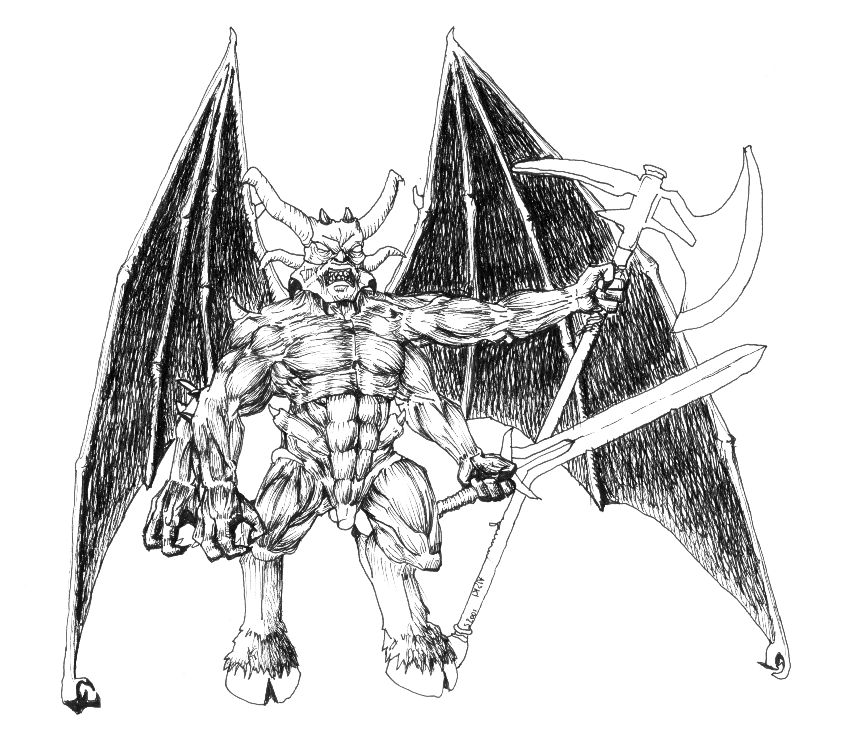
\includegraphics{arioch3.eps}
\end{center}
\end{figure*}

\demone{Arioch}{30}{Quinto Prisma}{Richiamabile} Appare come un grande
essere umanoide alto fino a 3 metri e mezzo. Appare nudo tranne che
per i foderi delle armi che porta con s\'e.

Ha quattro braccia con mani artigliate ed enormi ali membranose, che
possono raggiungere i 20 metri di apertura, terminanti con tre dita
artigliate.

Utilizza armi giganti solitamente ad una mano. Con le dita delle ali
pu\`o impugnare armi normali.


Ad una prima occhiata sembrerebbe avere la pelle rossa, in realt\`a
essa \`e assente; le fibre muscolari e i nervi sono direttamente
esposti all'aria, causandogli costantemente un atroce dolore di cui
Arioch gode.


Il suo volto appare costantemente animato da un'espressione mista di
dolore e piacere. I suoi occhi sono rossi e privi di pupille.  Il capo
\`e ornato da corna, sempre in numero pari e disposte
simmetricamente.

Arioch combatte utilizzando 2 Spade Bastarde giganti e 2 Alabarde
giganti. Talvolta abbandona le armi e combatte CAC utilizzando gli
artigli in grado di infliggere 2d8 PV/\-PSC di Danno; ama strappare
gli arti alle vittime e infilzarle sulle sue corna capaci di arrecare
2d8 PV/\-PSC di danno.

I suoi muscoli esposti all'aria sono comunque particolarmente
coriacei, tali da difenderlo come fossero una corazza di piastre (10
PP).

\carmostro{19+1d6}{15+1d10}{20+2d6}{20+1d10}{25+1d10}{25+1d8}{-1d10}{270}

\begin{parmostro}{Abilit\`a di Combattimento/TOT/Danno}
%%
\item CAC/AGI/2d8 
\item ATL/AGI/3d8+2 
\item ABL/AGI/3d8+1
\item AIA/AGI/3d8+1
\end{parmostro}

\begin{parmostro}{Attacchi Particolari/TOT/Danno}
%%
\item Corna/AGI/2d8
\end{parmostro}

\begin{parmostro}{Maestrie/TOT} 
%%
\item Spada Bastarda/AGI 
\item Alabarda/AGI
\end{parmostro}

\begin{parmostro}{Specifiche di AM/TOT/BON} 
%%
\item Presa/AGI/BON AGI
\end{parmostro}

\begin{parmostro}{Tecniche Speciali/TOT/BON} 
%%
\item Carica/20/+5
\end{parmostro}

\begin{parmostro}{Difese}
%%
\item Muscoli (PP 10)
\end{parmostro}

\begin{parmostro}{Poteri Speciali}
%%
\item Anima Diabolica
\item Fiamma Demoniaca
\item Schermo dell'Oblio
\item 13 Poteri a scelta del Master, con DR massima pari a 45.
\end{parmostro}

\demone{Belzeb\`u}{$\>$ 30}{Sesto Prisma}{Non Richiamabile} Appare
come una linea nera che disegna la sagoma di un umanoide alto sino a 2
m. Ha due sole dimensioni e qualora si volga di lato diventa
praticamente invisibile. Non lo si \`e mai sentito parlare e quando
intende comunicare disegna le parole nell'aria con la stessa linea che
delimita il suo corpo. Null'altro ci \`e dato sapere.

\demone{Baal}{$\>$ 30}{Settimo Prisma}{Non Richiamabile} Appare come un
giovane imberbe pallido e d'aspetto esile. Indossa esclusivamente un
perizoma. Il volto \`e contornato da lunghi riccioli neri e mostra
occhi chiarissimi; dal suo capo spuntano due piccole corna rivolte in
avanti. La sua voce sembra un sussurro. Si muove in maniera lenta e
indolente e sembra sempre afflitto da un profondo sentimento di
tristezza. Nessuno \`e sopravvissuto per fornire altre informazioni
su di lui.

\demone{Lo Dimonio}{$\>$ 30}{Ottavo Prisma}{Non Richiamabile}

La sua forma originaria \`e quella di un umano di etnia indefinita,
alto circa 180 cm, dalla carnagione olivastra.

Ha capelli neri portati lunghi o raccolti in una coda.  I suoi occhi
sono completamente neri.

La sua espressione \`e solitamente allegra e mostra un sorriso
malizioso. Dal capo spuntano due piccole corna nere che solitamente
nasconde fra i capelli. \`E solito abbigliarsi con vestiti lussuosi.
Porta sempre con s\'e un flauto di legno d'ebano capace di soggiogare
gli ascoltatori.

Pu\`o far nascere dalla sua schiena delle ali da rapace di colore
bianco atte al volo e la cui apertura raggiunge i 3.5 metri

\`E in grado di assumere le sembianze di qualsiasi altro demone. 

\subsubsection{I Demoni Generici}
\label{demonigenerici}

I demoni generici (introdotti a pagina \pageref{incantesimidemoni}) hanno le
forme pi\`u disparate. Solitamente, qualunque sia la forma base, vengono
estremizzate le caratteristiche proprie del demone specifico. 

\pinup{demonecorazza.eps}{Un demone generico (Corazza)}

Un demone che permette di udire avr\`a enormi orecchie, un demone
utile al trasporto avr\`a arti possenti, ecc.

\begin{description}
\item{\textbf{Potenza.}} la potenza \`e \textbf{pari alla DR}
  dell'incantesimo che manifesta il potere del demone.
  
\item{\textbf{Caratteristiche.}} Ognuna delle caratteristiche
  (BELlezza e CARisma escluse, determinate arbitrariamente dal Master)
  \`e pari a \textbf{1/2 della Potenza + 1d6}.
  
\item{\textbf{Energia.}} I PE utilizzabili per i poteri sono pari a
  \textbf{6 volte la Potenza}.
  
\item{\textbf{Poteri speciali.}}  Oltre al potere che si manifesta
  nell'incantesimo, i generici hanno un numero di poteri aggiuntivi a
  discrezione del Master pari ad \textbf{1/6 della Potenza}, ciascuno dei quali
  ha una \textbf{DR inferiore} alla Potenza.
  
\item{\textbf{Abilit\`a di Combattimento.}} I generici hanno un TOT nell'Abilit\`a
    \textbf{CAC pari ad AGI-3}.
\end{description}

\es{Gunnar vuole richiamare il Demone del
Gioco. L'incantesimo, che conferisce +5 all'abilit\`a Barare, ha DR 24. La
potenza del demone \`e 24; la DR dell'incantesimo che richiama uno di questi
demoni \`e 24 cio\`e 18 (DT) + 2 (Modificatori) + 24 (DB) - 20 (Modificatori)
= 24. Gunnar traccia il pentacolo e richiama il demone. Compare un essere umanoide
con la testa a forma di dado, le mani lunghissime e vestito di una tunica con
le maniche larghissime. Quest'essere, in base alla regola, avr\`a un VAL
alle caratteristiche pari a 24/2+1d6 cio\`e 12+1d6. 
 
Il Master tira i d6 ottenendo:
\begin{tabular}{ll}
  INT& 12 + 3 \\
  CONC& 12 + 5\\
  COS& 12 + 1\\ 
  AGI& 12 + 2 \\
  FOR& 12 + 5 \\ 
  OSS& 12 + 6 \\
\end{tabular}

Il demone avr\`a inoltre 144 PE, 4 poteri speciali aggiuntivi con DR
massima di 23 e un TOT in CAC pari a 14 (AGI)-3=11.

Il Master decide che i 4 poteri speciali aggiuntivi, oltre a Demone
del Gioco, del demone, sono: Acido, Corazza Infernale, Boccaglio e
Freccia Demoniaca}

\subsection{Gli Incantesimi}
\label{incdemonologia}
%----------------------------------------------------------------------------
\begin{spell}{Acido (Arkyox)}{Demonologia}{Attacco}{Danno Mirato}
%----------------------------------------------------------------------------
\descrizione{Dal mago parte uno spruzzo di acido che infligge ad un target a massimo 4 metri di distanza 1d6 PV/PSC di danno con base al TPC di 10.}
%% DR DA DT DB MOD PM PF PE TL
\incvalori{7}{23}{5}{15}{3}{7}{2}{23}{1}
\parametro{Danno}{1}{d6}{5}
\parametro{Base TPC}{10}{}{10}
\fineparametri
\gittata{4}{1}
\campo{1}{target}{2}
\durata{3 min}{0}
\end{spell}
%----------------------------------------------------------------------------
\begin{spell}{Ammorbidente (Rimmom)}{Demonologia}{Alterazione}{Variazione propriet\`a fisiche}
%----------------------------------------------------------------------------
\descrizione{Rende gli oggetti posti in un'area con un raggio di 4 metri, a distanza di massimo 10 metri dal mago, morbidi e inadatti a sorreggere pesi o a resistere agli urti. Il demone compare sotto forma di uno sciame di zanzare che succhiano materia dagli oggetti.}
%% DR DA DT DB MOD PM PF PE TL
\incvalori{31}{36}{15}{14}{7}{31}{10}{36}{5}
\parametro{Complessit\`a}{10}{}{10}
\parametro{Massa vivente}{100}{kg}{4}
\parametro{Massa non vivente}{0}{kg}{0}
\fineparametri
\gittata{10}{3}
\campo{4}{m}{4}
\durata{3 min}{0}
\end{spell}
%----------------------------------------------------------------------------
\begin{spell}{Anima diabolica (Foran)}{Demonologia}{Alterazione}{Creazione Esseri Viventi}
%----------------------------------------------------------------------------
\descrizione{Anima un oggetto (un monile, un'arma etc..) di 90 kg di peso massimo. L'incantesimo attribuisce 10 ad ogni caratteristica. L'oggetto si anima in 1d6 giorni.}
%% DR DA DT DB MOD PM PF PE TL
\incvalori{45}{50}{29}{23}{-2}{45}{15}{50}{7}
\parametro{Massa vivente}{90}{kg}{3}
\parametro{punti CAraTteristica}{80}{punti}{20}
\fineparametri
\gittatanulla
\campo{1}{target}{2}
\duratanulla
\azionetempo{1d6 giorni}{-3}
\end{spell}
%----------------------------------------------------------------------------
\begin{spell}{Aura demoniaca (Roneues)}{Demonologia}{Difesa}{Antimagia}
%----------------------------------------------------------------------------
\descrizione{Riveste il target di un'aura demoniaca rossastra che rende inattivo per 3 minuti qualsiasi incantesimo diretto al target con una base Antimagia di 20.}
%% DR DA DT DB MOD PM PF PE TL
\incvalori{22}{36}{15}{20}{1}{22}{7}{36}{3}
\parametro{Base antimagia}{20}{punti}{20}
\fineparametri
\gittatanulla
\campo{1}{target}{2}
\durata{3 min}{0}
\end{spell}
%----------------------------------------------------------------------------
\begin{spell}{Boccaglio (Gredlur)}{Demonologia}{Alterazione}{Modifica Anatomia per nuove funzioni}
%----------------------------------------------------------------------------
\descrizione{Un demone dalla forma di tubo telescopico (fino a 1 metro e 1/2) si collega con la bocca e il naso del target consentendogli di respirare sott'acqua o sotto terra. Il demone scompare dopo 3 minuti.}
%% DR DA DT DB MOD PM PF PE TL
\incvalori{22}{27}{15}{11}{1}{22}{7}{27}{3}
\parametro{Complessit\`a}{10}{}{10}
\parametro{Massa vivente}{5}{kg}{1}
\parametro{Fattore dimensione}{0}{unit\`a}{0}
\fineparametri
\gittatanulla
\campo{1}{target}{2}
\durata{3 min}{0}
\end{spell}
%----------------------------------------------------------------------------
\begin{spell}{Colonna di fuoco (Ighnar)}{Demonologia}{Attacco}{Danno Netto}
%----------------------------------------------------------------------------
\descrizione{Emette una fiammata che si propaga dal basso verso l'alto e che provoca 4d6 PV di danno su un'area di 2 metri di raggio situata fino a 10 metri dal mago. I danni possono essere dimezzati realizzando un TR a Diff. 18.}
%% DR DA DT DB MOD PM PF PE TL
\incvalori{18}{34}{21}{8}{5}{18}{6}{34}{3}
\parametro{Danno}{4}{d6}{8}
\fineparametri
\gittata{10}{3}
\campo{2}{m}{2}
\duratanulla
\end{spell}
%----------------------------------------------------------------------------
\begin{spell}{Corazza infernale (Reshpus)}{Demonologia}{Difesa}{Armatura}
%----------------------------------------------------------------------------
\descrizione{Un demone umanoide dal corpo cavo avvolge il corpo del target fornendogli 5 PP su tutto il corpo per 3 minuti.}
%% DR DA DT DB MOD PM PF PE TL
\incvalori{16}{30}{19}{10}{1}{16}{5}{30}{2}
\parametro{Protezione}{5}{PP}{10}
\fineparametri
\gittatanulla
\campo{1}{target}{2}
\durata{3 min}{0}
\end{spell}
%----------------------------------------------------------------------------
\begin{spell}{Decuria di Mammon}{Demonologia}{Evocazione}{Richiamo}
%----------------------------------------------------------------------------
\descrizione{Il mago evoca 10 demoni guerrieri Mammon. Il TV per il controllo viene effettuato separatamente da ciascuno di essi.}
%% DR DA DT DB MOD PM PF PE TL
\incvalori{22}{42}{18}{4}{20}{22}{7}{42}{3}
\parametro{Potenza della creatura}{4}{}{4}
\fineparametri
\gittata{1}{0}
\campo{10}{target}{20}
\durata{3 min}{0}
\end{spell}
%----------------------------------------------------------------------------
\begin{spell}{Demone del gioco (Abolam)}{Demonologia}{Alterazione}{Variazione abilit\`a fisica}
%----------------------------------------------------------------------------
\descrizione{Conferisce al target un bonus di +5 all'abilit\`a Barare per la durata della concentrazione del mago + 3 minuti.}
%% DR DA DT DB MOD PM PF PE TL
\incvalori{24}{29}{18}{5}{6}{24}{8}{29}{4}
\parametro{Variazione abilit\`a}{5}{punti}{5}
\fineparametri
\gittatanulla
\campo{1}{target}{2}
\durata{concentrazione+3 min}{5+0}
\end{spell}
%----------------------------------------------------------------------------
\begin{spell}{Difensore (Pazooso)}{Demonologia}{Difesa}{Protezione Magica}
%----------------------------------------------------------------------------
\descrizione{Il target viene protetto dal demone difensore che si manifesta come uno sciame di insetti vorticante che gli assorbe 4d6 PV di danno provocato dagli incantesimi di Attacco/Danno Netto. L'incantesimo ha durata 3 minuti.}
%% DR DA DT DB MOD PM PF PE TL
\incvalori{15}{29}{20}{8}{1}{15}{5}{29}{2}
\parametro{Protezione}{4}{d6}{8}
\fineparametri
\gittatanulla
\campo{1}{target}{2}
\durata{3 min}{0}
\end{spell}
%----------------------------------------------------------------------------
\begin{spell}{Doppelganger (Hutgin)}{Demonologia}{Controllo}{Miraggio completo}
%----------------------------------------------------------------------------
\descrizione{Un demone assume le sembianze del mago e si rende visibile ad una distanza di massimo 7 metri dal mago stesso senza peraltro potersi muovere al di fuori di un'area di 2 metri di raggio. Realizzando un TOSS a Diff. 20 ci si rende conto che si tratta di una copia, che sparisce se si realizza un TV a Diff. 20. La copia non pu\`o combattere. L'incantesimo dura 15 minuti.}
%% DR DA DT DB MOD PM PF PE TL
\incvalori{26}{36}{9}{20}{7}{26}{8}{36}{4}
\parametro{Difficolt\`a del TV e del TOSS}{20}{}{20}
\fineparametri
\gittata{7}{2}
\campo{2}{m}{2}
\durata{15 min}{3}
\end{spell}
%----------------------------------------------------------------------------
\begin{spell}{Evoca Alastor}{Demonologia}{Evocazione}{Richiamo}
%----------------------------------------------------------------------------
\descrizione{Evoca il demone guerriero Alastor per 3 minuti. Il mago pu\`o impartirgli ordini se vince un confronto di TV con esso.}
%% DR DA DT DB MOD PM PF PE TL
\incvalori{14}{34}{18}{14}{2}{14}{4}{34}{2}
\parametro{Potenza della creatura}{14}{}{14}
\fineparametri
\gittata{1}{0}
\campo{1}{target}{2}
\durata{3 min}{0}
\end{spell}
%----------------------------------------------------------------------------
\begin{spell}{Evoca Ammon}{Demonologia}{Evocazione}{Richiamo}
%----------------------------------------------------------------------------
\descrizione{Evoca il demone guerriero Ammon per 3 minuti. Il mago pu\`o impartirgli ordini se vince un confronto di TV con esso.}
%% DR DA DT DB MOD PM PF PE TL
\incvalori{9}{29}{18}{9}{2}{9}{3}{29}{1}
\parametro{Potenza della creatura}{9}{}{9}
\fineparametri
\gittata{1}{0}
\campo{1}{target}{2}
\durata{3 min}{0}
\end{spell}
%----------------------------------------------------------------------------
\begin{spell}{Evoca Arioch}{Demonologia}{Evocazione}{Richiamo}
%----------------------------------------------------------------------------
\descrizione{Evoca il demone guerriero Arioch per 3 minuti. Il mago pu\`o impartirgli ordini se vince un confronto di TV con esso.}
%% DR DA DT DB MOD PM PF PE TL
\incvalori{30}{50}{18}{30}{2}{30}{10}{50}{5}
\parametro{Potenza della creatura}{30}{}{30}
\fineparametri
\gittata{1}{0}
\campo{1}{target}{2}
\durata{3 min}{0}
\end{spell}
%----------------------------------------------------------------------------
\begin{spell}{Evoca Mammon}{Demonologia}{Evocazione}{Richiamo}
%----------------------------------------------------------------------------
\descrizione{Evoca il demone guerriero Mammon per 3 minuti. Il mago pu\`o impartirgli ordini se vince un confronto di TV con esso.}
%% DR DA DT DB MOD PM PF PE TL
\incvalori{4}{24}{18}{4}{2}{4}{1}{24}{1}
\parametro{Potenza della creatura}{4}{}{4}
\fineparametri
\gittata{1}{0}
\campo{1}{target}{2}
\durata{3 min}{0}
\end{spell}
%----------------------------------------------------------------------------
\begin{spell}{Evoca Strayesor}{Demonologia}{Evocazione}{Richiamo}
%----------------------------------------------------------------------------
\descrizione{Evoca il demone guerriero Strayesor per 3 minuti. Il mago pu\`o impartirgli ordini se vince un confronto di TV con esso.}
%% DR DA DT DB MOD PM PF PE TL
\incvalori{19}{39}{18}{19}{2}{19}{6}{39}{3}
\parametro{Potenza della creatura}{19}{}{19}
\fineparametri
\gittata{1}{0}
\campo{1}{target}{2}
\durata{3 min}{0}
\end{spell}
%----------------------------------------------------------------------------
\begin{spell}{Fascino satanico (Kham)}{Demonologia}{Controllo}{Comando}
%----------------------------------------------------------------------------
\descrizione{Gli esseri situati all'interno di un'area di un metro di raggio che non realizzano un TV a Diff. 20 vengono affascinati irresistibilmente dal mago per 3 minuti.}
%% DR DA DT DB MOD PM PF PE TL
\incvalori{22}{32}{11}{20}{1}{22}{7}{32}{3}
\parametro{Difficolt\`a del TV}{20}{}{20}
\fineparametri
\gittata{1}{0}
\campo{1}{m}{1}
\durata{3 min}{0}
\end{spell}
%----------------------------------------------------------------------------
\begin{spell}{Fiamma demoniaca (Rahouart)}{Demonologia}{Attacco}{Danno Netto}
%----------------------------------------------------------------------------
\descrizione{Fa partire dal mago una fiammata larga 20 metri che distrugge tutto ci\`o su cui passa, per una gittata di massimo 19 metri, esplodendo poi su un'area di 10 metri di raggio e provocando a tutti gli oggetti investiti un danno di 10d6 PV. Le vittime possono dimezzare il danno realizzando un TR a Diff. 30. La fiamma pu\`o produrre danni addizionali.}
%% DR DA DT DB MOD PM PF PE TL
\incvalori{44}{60}{21}{20}{19}{44}{14}{60}{7}
\parametro{Danno}{10}{d6}{20}
\fineparametri
\gittata{19}{6}
\azionegittata
\campo{10}{m}{10}
\duratanulla
\end{spell}
%----------------------------------------------------------------------------
\begin{spell}{Filamento adesivo (Poimon)}{Demonologia}{Difesa}{Parata}
%----------------------------------------------------------------------------
\descrizione{Dal corpo del target si diparte un filamento adesivo atto a parare un colpo con Base TPD 5. Dopo 3 minuti o dopo una parata il filamento scompare.}
%% DR DA DT DB MOD PM PF PE TL
\incvalori{9}{23}{15}{7}{1}{9}{3}{23}{1}
\parametro{Base TPD}{5}{punti}{5}
\parametro{Parate}{1}{}{2}
\fineparametri
\gittatanulla
\campo{1}{target}{2}
\durata{3 min}{0}
\end{spell}
%----------------------------------------------------------------------------
\begin{spell}{Freccia demoniaca (Dreayn)}{Demonologia}{Attacco}{Danno Mirato}
%----------------------------------------------------------------------------
\descrizione{Fa scaturire dal mago un piccolo demone simile ad una larva dotata di zanne che si scaglia sul target, distante massimo 10 metri, mordendolo e infliggendogli 1d6 PV/PSC di danno. La base TPC \`e 15.}
%% DR DA DT DB MOD PM PF PE TL
\incvalori{14}{30}{5}{20}{5}{14}{4}{30}{2}
\parametro{Danno}{1}{d6}{5}
\parametro{Base TPC}{15}{}{15}
\fineparametri
\gittata{10}{3}
\campo{1}{target}{2}
\duratanulla
\end{spell}
%----------------------------------------------------------------------------
\begin{spell}{Globo demoniaco (Kira)}{Demonologia}{Difesa}{Antimagia}
%----------------------------------------------------------------------------
\descrizione{Crea un globo di luce demoniaca rossastra di 1 metro di raggio per 3 minuti. Qualunque incantesimo diretto ad esseri od oggetti all'interno del globo sar\`a neutralizzato con una base antimagia di 20. Il mago pu\`o creare il globo fino a 1 metro di distanza da s\'e.}
%% DR DA DT DB MOD PM PF PE TL
\incvalori{22}{36}{15}{20}{1}{22}{7}{36}{3}
\parametro{Base antimagia}{20}{punti}{20}
\fineparametri
\gittata{1}{0}
\campo{1}{m}{1}
\durata{3 min}{0}
\end{spell}
%----------------------------------------------------------------------------
\begin{spell}{Guanto (Adramelek)}{Demonologia}{Attacco}{Morte}
%----------------------------------------------------------------------------
\descrizione{Il target che non realizza un TR a Diff. 20 viene rivoltato come un guanto, morendo istantaneamente. Il corpo torna intatto dopo un incantesimo di resurrezione.}
%% DR DA DT DB MOD PM PF PE TL
\incvalori{23}{39}{18}{20}{1}{23}{7}{39}{3}
\parametro{Difficolt\`a del TR}{20}{}{20}
\fineparametri
\gittatanulla
\campo{1}{target}{2}
\duratanulla
\end{spell}
%----------------------------------------------------------------------------
\begin{spell}{Guaritore (Baribars)}{Demonologia}{Difesa}{Cura}
%----------------------------------------------------------------------------
\descrizione{Con questo incantesimo, il mago \`e in grado, grazie al demone Guaritore, di curare 3d6 PV/PSC di danno a tutti gli esseri viventi posti ad una distanza massima di 1 metro da lui ed in un'area di 1 metro di raggio. L'incantesimo lascia tracce visibili della cura sotto forma di  escrescenze cutanee o simili.}
%% DR DA DT DB MOD PM PF PE TL
\incvalori{14}{28}{21}{6}{1}{14}{4}{28}{2}
\parametro{Riparazione}{3}{d6}{6}
\fineparametri
\gittata{1}{0}
\campo{1}{m}{1}
\duratanulla
\end{spell}
%----------------------------------------------------------------------------
\begin{spell}{Individua demoni (Zebuliel)}{Demonologia}{Informazione}{Divinazione}
%----------------------------------------------------------------------------
\descrizione{L'incantesimo individua la presenza di uno o pi\`u demoni nel raggio di 10 metri, senza indicarne la collocazione.}
%% DR DA DT DB MOD PM PF PE TL
\incvalori{18}{28}{9}{10}{9}{18}{6}{28}{3}
\parametro{DIFF reperimento informazione}{10}{}{10}
\parametro{Previsione}{0}{ore}{0}
\fineparametri
\gittatanulla
\campo{10}{m}{10}
\durata{3 min}{0}
\end{spell}
%----------------------------------------------------------------------------
\begin{spell}{Intercettatore (Zyunsak)}{Demonologia}{Difesa}{Parata}
%----------------------------------------------------------------------------
\descrizione{Il target viene protetto dal Demone intercettatore in grado di parare 5 attacchi fisici o di Attacco/Danno Mirato con una base di parata di 15. Il demone svanisce dopo 3 minuti oppure dopo aver parato 5 attacchi.}
%% DR DA DT DB MOD PM PF PE TL
\incvalori{27}{41}{15}{25}{1}{27}{9}{41}{4}
\parametro{Base TPD}{15}{punti}{15}
\parametro{Parate}{5}{}{10}
\fineparametri
\gittatanulla
\campo{1}{target}{2}
\durata{3 min}{0}
\end{spell}
%----------------------------------------------------------------------------
\begin{spell}{Macellaio (Greayn)}{Demonologia}{Attacco}{Danno Mirato}
%----------------------------------------------------------------------------
\descrizione{La vittima viene scuoiata nel punto di contatto con la mano dell'usufruitore, ricevendo 3d6 PV/PSC di danno. Infligge danni addizionali da emorragia. L'usufruitore potrebbe dover realizzare un TPC con l'abilit\`a CAC.}
%% DR DA DT DB MOD PM PF PE TL
\incvalori{5}{21}{5}{15}{1}{5}{1}{21}{1}
\parametro{Danno}{3}{d6}{15}
\parametro{Base TPC}{0}{}{0}
\fineparametri
\gittatanulla
\campo{1}{target}{2}
\durata{3 min}{0}
\end{spell}
%----------------------------------------------------------------------------
\begin{spell}{Mantici (Iblis)}{Demonologia}{Alterazione}{Spostamento 3 dimensioni}
%----------------------------------------------------------------------------
\descrizione{Alcuni piccoli demoni che ingoiano ed emettono aria si attaccano al corpo del target del peso massimo di 90 kg e con un equipaggiamento di massimo 100 kg, consentendogli di volare per 3 minuti a 100 km/h.}
%% DR DA DT DB MOD PM PF PE TL
\incvalori{29}{34}{19}{14}{1}{29}{9}{34}{4}
\parametro{Massa vivente}{90}{kg}{3}
\parametro{Velocit\`a}{100}{km/h}{10}
\parametro{Massa non vivente}{90}{kg}{1}
\fineparametri
\gittatanulla
\campo{1}{target}{2}
\durata{3 min}{0}
\end{spell}
%----------------------------------------------------------------------------
\begin{spell}{Messaggero (Belialys)}{Demonologia}{Informazione}{Trasmissione+Ricezione}
%----------------------------------------------------------------------------
\descrizione{Un demone messaggero recapita istantaneamente un messaggio scritto di poche pagine ad un target posto ad una distanza massima di 10 km, ricevendo una eventuale risposta e riportandola al mago.}
%% DR DA DT DB MOD PM PF PE TL
\incvalori{26}{36}{15}{20}{1}{26}{8}{36}{4}
\parametro{Complessit\`a}{4}{}{4}
\parametro{Distanza}{10000}{m}{16}
\fineparametri
\gittatanulla
\campo{1}{target}{2}
\duratanulla
\end{spell}
%----------------------------------------------------------------------------
\begin{spell}{Patto Demoniaco (Haflain)}{Demonologia}{Controllo}{Comando}
%----------------------------------------------------------------------------
\descrizione{Con questo incantesimo il mago pu\`o, grazie al demone persuasore, obbligare tutti coloro che si trovano alla distanza massima di 1 metro e nell'area di 1 metro di raggio, ad eseguire un ordine a suo piacimento, se questi non realizzano un TV a Diff. 20. Per tutte le vittime l'ordine \`e lo stesso.}
%% DR DA DT DB MOD PM PF PE TL
\incvalori{22}{32}{11}{20}{1}{22}{7}{32}{3}
\parametro{Difficolt\`a del TV}{20}{}{20}
\fineparametri
\gittata{1}{0}
\campo{1}{m}{1}
\durata{3 min}{0}
\end{spell}
%----------------------------------------------------------------------------
\begin{spell}{Pelle robusta (Tsu Nyao)}{Demonologia}{Difesa}{Armatura}
%----------------------------------------------------------------------------
\descrizione{La pelle del target si ingrossa e si ricopre di escrescenze cornee che la rendono dura e dotata di 1 PP, per 7 minuti.}
%% DR DA DT DB MOD PM PF PE TL
\incvalori{9}{23}{19}{2}{2}{9}{3}{23}{1}
\parametro{Protezione}{1}{PP}{2}
\fineparametri
\gittatanulla
\campo{1}{target}{2}
\durata{7 min}{1}
\end{spell}
%----------------------------------------------------------------------------
\begin{spell}{Pelle viscida (Abludar)}{Demonologia}{Alterazione}{Variazione abilit\`a fisica}
%----------------------------------------------------------------------------
\descrizione{Il target viene rivestito da uno strato di liquido viscoso e scivoloso che gli conferisce un bonus di +5 al TOT della Specifica di AM ``divincolarsi''.}
%% DR DA DT DB MOD PM PF PE TL
\incvalori{19}{24}{18}{5}{1}{19}{6}{24}{3}
\parametro{Variazione abilit\`a}{5}{punti}{5}
\fineparametri
\gittatanulla
\campo{1}{target}{2}
\durata{3 min}{0}
\end{spell}
%----------------------------------------------------------------------------
\begin{spell}{Portatore di dolore (Koim)}{Demonologia}{Informazione}{Variazione abilit\`a mentale}
%----------------------------------------------------------------------------
\descrizione{Il demone conferisce al target un bonus di +5 all'abilit\`a Torture per 15 minuti.}
%% DR DA DT DB MOD PM PF PE TL
\incvalori{17}{27}{18}{5}{4}{17}{5}{27}{2}
\parametro{Variazione abilit\`a}{5}{punti}{5}
\fineparametri
\gittatanulla
\campo{1}{target}{2}
\durata{15 min}{3}
\end{spell}
%----------------------------------------------------------------------------
\begin{spell}{Possesso diabolico (Behemoth)}{Demonologia}{Controllo}{Possessione}
%----------------------------------------------------------------------------
\descrizione{L'usufruitore si impossessa del corpo di un target per 3 minuti, se questi non realizza un TV a Diff. 20.}
%% DR DA DT DB MOD PM PF PE TL
\incvalori{22}{32}{11}{20}{1}{22}{7}{32}{3}
\parametro{Difficolt\`a del TV}{20}{}{20}
\fineparametri
\gittatanulla
\campo{1}{target}{2}
\durata{3 min}{0}
\end{spell}
%----------------------------------------------------------------------------
\begin{spell}{Protezione dai Demoni I}{Demonologia}{Evocazione}{Protezione}
%----------------------------------------------------------------------------
\descrizione{Viene creata, attorno ad un punto distante al massimo 4 metri dal mago, un'area di 3 metri di raggio all'interno della quale i Demoni di potenza uguale o inferiore a 9 non possono entrare se non realizzando un TV a Diff. 19. Realizzando il TV le creature potranno avanzare di 1 metro, subendo 1d6 PV di danno per ogni metro all'interno dell'area, L'incantesimo scompare se il mago attacca le creature dalle quali si sta proteggendo. Per ogni metro all'interno dell'area il TV delle creature \`e penalizzato di -1. L'incantesimo perdura per 3 minuti.}
%% DR DA DT DB MOD PM PF PE TL
\incvalori{3}{23}{10}{9}{4}{3}{1}{23}{1}
\parametro{Potenza della creatura}{9}{}{9}
\fineparametri
\gittata{4}{1}
\campo{3}{m}{3}
\durata{3 min}{0}
\end{spell}
%----------------------------------------------------------------------------
\begin{spell}{Protezione dai Demoni II}{Demonologia}{Evocazione}{Protezione}
%----------------------------------------------------------------------------
\descrizione{Viene creata, attorno ad un punto distante al massimo 4 metri dal mago, un'area di 3 metri di raggio all'interno della quale i Demoni di potenza uguale o inferiore a 19 non possono entrare se non realizzando un TV a Diff. 29. Realizzando il TV le creature potranno avanzare di 1 metro, subendo 1d6 PV di danno per ogni metro all'interno dell'area, L'incantesimo scompare se il mago attacca le creature dalle quali si sta proteggendo. Per ogni metro all'interno dell'area il TV delle creature \`e penalizzato di -1. L'incantesimo perdura per 3 minuti.}
%% DR DA DT DB MOD PM PF PE TL
\incvalori{13}{33}{10}{19}{4}{13}{4}{33}{2}
\parametro{Potenza della creatura}{19}{}{19}
\fineparametri
\gittata{4}{1}
\campo{3}{m}{3}
\durata{3 min}{0}
\end{spell}
%----------------------------------------------------------------------------
\begin{spell}{Protezione dai Demoni III}{Demonologia}{Evocazione}{Protezione}
%----------------------------------------------------------------------------
\descrizione{Viene creata, attorno ad un punto distante al massimo 4 metri dal mago, un'area di 3 metri di raggio all'interno della quale i Demoni di potenza uguale o inferiore a 30 non possono entrare se non realizzando un TV a Diff. 40. Realizzando il TV le creature potranno avanzare di 1 metro, subendo 1d6 PV di danno per ogni metro all'interno dell'area, L'incantesimo scompare se il mago attacca le creature dalle quali si sta proteggendo. Per ogni metro all'interno dell'area il TV delle creature \`e penalizzato di -1. L'incantesimo perdura per 3 minuti.}
%% DR DA DT DB MOD PM PF PE TL
\incvalori{24}{44}{10}{30}{4}{24}{8}{44}{4}
\parametro{Potenza della creatura}{30}{}{30}
\fineparametri
\gittata{4}{1}
\campo{3}{m}{3}
\durata{3 min}{0}
\end{spell}
%----------------------------------------------------------------------------
\begin{spell}{Rostro (Morkooya)}{Demonologia}{Alterazione}{Modifica Danni anatomia/armi}
%----------------------------------------------------------------------------
\descrizione{Il braccio del target viene rivestito da una superficie dura, rugosa e dotata di punte acuminate, rendendo il danno base di Pugno pari a 1d4 + 2d6. L'incantesimo dura 3 minuti.}
%% DR DA DT DB MOD PM PF PE TL
\incvalori{27}{32}{20}{11}{1}{27}{9}{32}{4}
\parametro{Danno}{2}{d6}{10}
\parametro{Massa}{5}{kg}{1}
\fineparametri
\gittatanulla
\campo{1}{target}{2}
\durata{3 min}{0}
\end{spell}
%----------------------------------------------------------------------------
\begin{spell}{Schermo dell'Oblio (Krisral)}{Demonologia}{Difesa}{Deviazione}
%----------------------------------------------------------------------------
\descrizione{Il target viene protetto da uno schermo che para tutti gli attacchi fisici o di Attacco/Danno Mirato con base TPD 20. L'incantesimo dura 3 minuti.}
%% DR DA DT DB MOD PM PF PE TL
\incvalori{32}{46}{25}{20}{1}{32}{10}{46}{5}
\parametro{Base TPD}{20}{punti}{20}
\fineparametri
\gittatanulla
\campo{1}{target}{2}
\durata{3 min}{0}
\end{spell}
%----------------------------------------------------------------------------
\begin{spell}{Seduttore (Azazel)}{Demonologia}{Alterazione}{Variazione abilit\`a fisica}
%----------------------------------------------------------------------------
\descrizione{Conferisce al target un bonus di +5 all'abilit\`a Sedurre per 15 minuti.}
%% DR DA DT DB MOD PM PF PE TL
\incvalori{22}{27}{18}{5}{4}{22}{7}{27}{3}
\parametro{Variazione abilit\`a}{5}{punti}{5}
\fineparametri
\gittatanulla
\campo{1}{target}{2}
\durata{15 min}{3}
\end{spell}
%----------------------------------------------------------------------------
\begin{spell}{Sguardo di fuoco (Ayperos)}{Demonologia}{Alterazione}{Modifica Anatomia per nuove funzioni}
%----------------------------------------------------------------------------
\descrizione{Gli occhi del target saranno modificati in modo da vedere al buio. Gli occhi brilleranno di una sinistra luce rossastra. L'incantesimo dura a concentrazione pi\`u 3 minuti.}
%% DR DA DT DB MOD PM PF PE TL
\incvalori{22}{27}{15}{6}{6}{22}{7}{27}{3}
\parametro{Complessit\`a}{5}{}{5}
\parametro{Massa vivente}{1}{kg}{1}
\parametro{Fattore dimensione}{0}{unit\`a}{0}
\fineparametri
\gittatanulla
\campo{1}{target}{2}
\durata{concentrazione+3 min}{5+0}
\end{spell}
%----------------------------------------------------------------------------
\begin{spell}{Sottomissione Demoni I}{Demonologia}{Evocazione}{Controllo}
%----------------------------------------------------------------------------
\descrizione{Consente di sottomettere ai propri ordini un demone di potenza massima pari a 9 per 3 minuti. Il mago pu\`o impartirgli ordini se vince un confronto di TV con esso se \`e un essere errante, o con chi lo domina se \`e controllato..}
%% DR DA DT DB MOD PM PF PE TL
\incvalori{6}{26}{14}{9}{3}{6}{2}{26}{1}
\parametro{Potenza della creatura}{9}{}{9}
\fineparametri
\gittata{4}{1}
\campo{1}{target}{2}
\durata{3 min}{0}
\end{spell}
%----------------------------------------------------------------------------
\begin{spell}{Sottomissione Demoni II}{Demonologia}{Evocazione}{Controllo}
%----------------------------------------------------------------------------
\descrizione{Consente di sottomettere ai propri ordini un demone di potenza massima pari a 19 per 3 minuti. Il mago pu\`o impartirgli ordini se vince un confronto di TV con esso se \`e un essere errante, o con chi lo domina se \`e controllato..}
%% DR DA DT DB MOD PM PF PE TL
\incvalori{16}{36}{14}{19}{3}{16}{5}{36}{2}
\parametro{Potenza della creatura}{19}{}{19}
\fineparametri
\gittata{4}{1}
\campo{1}{target}{2}
\durata{3 min}{0}
\end{spell}
%----------------------------------------------------------------------------
\begin{spell}{Sottomissione Demoni III}{Demonologia}{Evocazione}{Controllo}
%----------------------------------------------------------------------------
\descrizione{Consente di sottomettere ai propri ordini un demone di potenza massima pari a 30 per 3 minuti. Il mago pu\`o impartirgli ordini se vince un confronto di TV con esso se \`e un essere errante, o con chi lo domina se \`e controllato..}
%% DR DA DT DB MOD PM PF PE TL
\incvalori{27}{47}{14}{30}{3}{27}{9}{47}{4}
\parametro{Potenza della creatura}{30}{}{30}
\fineparametri
\gittata{4}{1}
\campo{1}{target}{2}
\durata{3 min}{0}
\end{spell}
%----------------------------------------------------------------------------
\begin{spell}{Sparizione (Gusartan)}{Demonologia}{Alterazione}{Teletrasporto standard}
%----------------------------------------------------------------------------
\descrizione{Teletrasporta il target a 100 metri di distanza in un punto in cui il demonologo \`e gi\`a stato. Il target deve pesare al massimo 90 kg ed avere non pi\`u di 100 kg di equipaggiamento. Il target pu\`o subire danni a discrezione del Master se il punto di destinazione \`e inagibile o gi\`a occupato.}
%% DR DA DT DB MOD PM PF PE TL
\incvalori{29}{34}{19}{14}{1}{29}{9}{34}{4}
\parametro{Massa vivente}{90}{kg}{3}
\parametro{Massa non vivente}{100}{kg}{1}
\parametro{Distanza di spostamento}{100}{m}{10}
\fineparametri
\gittatanulla
\campo{1}{target}{2}
\duratanulla
\end{spell}
%----------------------------------------------------------------------------
\begin{spell}{Suggeritore (Wala)}{Demonologia}{Informazione}{Variazione CONoscenza}
%----------------------------------------------------------------------------
\descrizione{Il target rester\`a in contatto col demone suggeritore, facendo aumentare di +1 la caratteristica CON, per il tempo in cui il mago terr\`a la concentrazione pi\`u 3 minuti.}
%% DR DA DT DB MOD PM PF PE TL
\incvalori{21}{31}{19}{6}{6}{21}{7}{31}{3}
\parametro{Variazione caratteristica}{1}{punto}{6}
\fineparametri
\gittatanulla
\campo{1}{target}{2}
\durata{concentrazione+3 min}{5+0}
\end{spell}
%----------------------------------------------------------------------------
\begin{spell}{Tentacoli (Belfagor)}{Demonologia}{Difesa}{Scudo antidinamico}
%----------------------------------------------------------------------------
\descrizione{L'usufruitore viene ricoperto da piccolissimi tentacoli che gli permettono di dimezzare tutti i danni da botta, da punta e da taglio, compresi quelli prodotti dagli incantesimi di Attacco/Danno Mirato, che gli vengono inflitti.}
%% DR DA DT DB MOD PM PF PE TL
\incvalori{18}{32}{21}{10}{1}{18}{6}{32}{3}
\parametro{Divisore}{2}{unit\`a}{10}
\fineparametri
\gittatanulla
\campo{1}{target}{2}
\durata{3 min}{0}
\end{spell}
%----------------------------------------------------------------------------
\begin{spell}{Tentazione (Schax)}{Demonologia}{Controllo}{Illusione completa}
%----------------------------------------------------------------------------
\descrizione{Mostra alle vittime situate in un'area di 1 metro di raggio distante fino a 1 metro dal mago immagini suadenti e ammaliatrici, che verranno percepite anche con tatto, olfatto, udito. Un TOSS a Diff. 20 render\`a consapevoli le vittime che le immagini non sono reali. In seguito, un TV a Diff. 20 potr\`a farle scomparire.}
%% DR DA DT DB MOD PM PF PE TL
\incvalori{20}{30}{9}{20}{1}{20}{6}{30}{3}
\parametro{Difficolt\`a del TV e del TOSS}{20}{}{20}
\fineparametri
\gittata{1}{0}
\campo{1}{m}{1}
\durata{3 min}{0}
\end{spell}
%----------------------------------------------------------------------------
\begin{spell}{Tipografo (Pruslas)}{Demonologia}{Informazione}{Registrazione}
%----------------------------------------------------------------------------
\descrizione{Ricopia un breve libro su un mazzo di fogli bianchi o simili, aggiungendo disegni osceni o raccapriccianti alla copia. La copia termina in 1d6 ore ed \`e permanente. L'incantesimo non ricopia correttamente i libri magici.}
%% DR DA DT DB MOD PM PF PE TL
\incvalori{33}{43}{22}{5}{16}{33}{11}{43}{5}
\parametro{Complessit\`a}{5}{}{5}
\fineparametri
\gittatanulla
\campo{1}{target}{2}
\durata{permanente }{15}
\end{spell}
%----------------------------------------------------------------------------
\begin{spell}{Violinista (Shentsow)}{Demonologia}{Attacco}{Stordimento}
%----------------------------------------------------------------------------
\descrizione{Pizzica i nervi delle vittime che si trovano in un'area di 2 metri di raggio distante fino a 10 metri dal target come fossero corde di violino, causandone lo stordimento (inabilitazione per il round in corso e quello successivo).}
%% DR DA DT DB MOD PM PF PE TL
\incvalori{18}{34}{9}{20}{5}{18}{6}{34}{3}
\parametro{Difficolt\`a del TR}{20}{}{20}
\fineparametri
\gittata{10}{3}
\campo{2}{m}{2}
\duratanulla
\end{spell}
%----------------------------------------------------------------------------
\begin{spell}{Zanna di luce (Guang Ya)}{Demonologia}{Attacco}{Danno Mirato}
%----------------------------------------------------------------------------
\descrizione{Un demone dalla forma della testa di un serpente luminescente infligge 2d6 PV/PSC di danno ad un target che si trova a massimo 7 metri dal mago. Il TPC \`e pari a 12.}
%% DR DA DT DB MOD PM PF PE TL
\incvalori{15}{31}{5}{22}{4}{15}{5}{31}{2}
\parametro{Danno}{2}{d6}{10}
\parametro{Base TPC}{12}{}{12}
\fineparametri
\gittata{7}{2}
\campo{1}{target}{2}
\duratanulla
\end{spell}

\vfill
\fi
%%---------------------------------------------------------------------------
\section{Elementalismo} 
%%---------------------------------------------------------------------------
\Simbolo{simb_ele.eps}

Parte del regno Memath, l'Elementalismo, detta Via degli Elementi in
Elfico, o Magia della Materia in Novese, governa i quattro elementi
Aria, Fuoco, Acqua e Terra.

Simbolo degli elementalisti \`e un triangolo equilatero,
diviso in quattro bande orizzontali, con il vertice rivolto verso il
basso.

\subsection{Dominio} 

L'Elementalismo domina ed attinge il suo potere dall'essenza degli
elementi, ordinati gerarchicamente col seguente schema: Aria (base),
Fuoco, Acqua e Pietra (apice), in modo che siano potenzialmente pi\`u
forti gli elementi che per affinit\`a sono pi\`u vicini alla Terra.
L'aria, di per s\'e, \`e gi\`a al di sopra della Terra; il Fuoco ha
sempre contatti diretti col terreno, mentre l'acqua \`e di natura
pi\`u pesante dell'aria e tender\`a a restare a contatto con la terra.
Inoltre, provate a soffiare dell'aria in una polla d'acqua: essa
risalir\`a rapidamente per riunirsi all'aria che si trova sopra la
polla.

La Pietra conferisce il
potere maggiore in quanto elemento primario del Piano Materiale. 

Tutti
gli incantesimi di questa scuola devono essere correlati con almeno
uno dei quattro elementi.

\subsection{Limiti e peculiarit\`a} 

Gli usufruitori che conoscono questa scuola sono gli unici a poter
evocare le creature elementali, e solo queste. Si pu\`o evocare un
elementale solo se l'elemento da cui prende essenza esiste in grande
quantit\`a o predominanza nel luogo dell'evocazione. Non si possono
evocare gli elementali dell'aria in luoghi senza contatti con
l'esterno. Non si possono evocare elementali della pietra in mare, sui
laghi o sui corsi d'acqua, e tanto meno in aria. Gli elementali del
fuoco si possono chiamare soltanto in prossimit\`a di una fiamma
viva, delle dimensioni di almeno un focolare, gli elementali
dell'acqua solo in prossimit\`a di specchi o corsi d'acqua, o quando
piove.

\subsection{Potenzialit\`a}

\begin{tabular}{lc}
Evocazione&11\\
Alterazione& 16\\
Controllo& 5\\ 
Informazione& 9\\
Difesa& 14\\
Attacco& 20\\ 
\end{tabular}

\subsection{Leggi dell'uso}
\begin{enumerate}\itemsep -6pt
\item Non lasciare liberi gli elementali
\item Non causare catastrofi 
\end{enumerate}

\iffullversion
\subsection{Gli Elementali} 

Gli Elementali
sono le essenze vitali dei quattro elementi: Fuoco, Aria, Acqua e Pietra e possono
essere richiamati da un Elementalista con un incantesimo di Evocazione. 

Un Elementalista pu\`o richiamare un determinato tipo di Elementale
(dell'aria, del Fuoco, dell'acqua e della Pietra) soltanto se nel
luogo dell'Evocazione \`e presente in grande quantit\`a l'elemento
da cui l'essere prende vita, come limite e peculiarit\`a della
Scuola di Elementalismo.

Esiste un diverso tipo di Elementale per ognuno dei quattro elementi,
ed ogni tipo ha caratteristiche proprie. Ogni tipo di Elementale ha
come dominio solo l'elemento da cui trae origine. Per esempio, un
Elementale dell'acqua non ha poteri sul fuoco, la terra o l'aria, ecc.
Per questo motivo i poteri Evocazione Elementali, Controllo Elementali
e Parlare agli Elementi, riguardano solo l'elemento corrispondente al
Tipo di Elementale. 

Ogni Elementale \`e immune agli attacchi
portati con il suo elemento (cos\`{\i} lanciare una Palla di Fuoco contro un
elementale del Fuoco non sortir\`a alcun effetto) ed agli incantesimi di
morte che colpiscono gli esseri viventi. 

Un Elementale pu\`o essere distrutto portando a 0 i PSC del Torace o
della Testa oppure facendo in modo che arrivi a 0 PV. Quando viene
distrutto l'elementale scompare.

Quando viene evocato e sconfitto nel confronto di TV, l'Elementale
tende ad eseguire il comando impartitogli alla lettera e senza
rifletterci troppo. Se vince il confronto di TV, l'Elementale
solitamente ritorna nell'elemento da cui ha preso vita senza creare
ulteriori problemi.

L'Elementale \`e in contatto telepatico con l'Evocatore per tutta
la durata dell'Evocazione, e pu\`o comunicare solo con costui.

Gli Elementali vengono divisi in 3 categorie a seconda della
loro Potenza: Elementali Minori (Evocabili), Elementali Maggiori
(Evocabili), Elementali Superiori (Non Evocabili).

\elementale{Elementale dell'aria Minore}{8}{Richiamabile}

\`E un essere traslucido fatto d'aria, dalla forma umanoide, alto
circa 150 cm, con al posto delle gambe un vortice che gli permette di
muoversi fluttuando, alla velocit\`a massima di 20 metri per Round.
Non brandisce armi e combatte a mani nude. 

\pinup{el_aria2.eps}{Elementale dell'aria}

Il suo TOT in CAC \`e pari al suo valore in AGI. 

\carmostro{10+2d6}{4+2d8}{15+1d10}{15+1d10}{15+1d10}{4+2d8}{-}{90}

\begin{parmostro}{Abilit\`a di Combattimento/TOT/Danno} 
\item CAC/AGI/Danno normale
\end{parmostro}

\begin{parmostro}{Difese} 
\item Immunit\`a ad attacchi con l'aria
\end{parmostro}

\begin{parmostro}{Poteri Speciali} 
\item Controllo Aria
\item Sciabola di Vento
\item Sfera di Vuoto
\item Ululato di Vento
\end{parmostro}

\elementale{Elementale del Fuoco Minore}{10}{Richiamabile} 

\`E un essere che trae vita dal fuoco ed ha le sembianze di una grossa
fiamma umanoide alta circa 150 cm. Se il suo corpo viene toccato, il
fuoco che lo avvolge infligge alla vittima 1d6 PV/\-PSC di danno, per
questo motivo i suoi attacchi fisici, oltre al danno normale
infliggono ulteriori 1d6 PV/\-PSC.

Non brandisce armi ed il TOT nella sua abilit\`a CAC \`e pari al
valore della sua AGI. Pu\`o cambiare le proprie dimensioni col
potere Dimensioni Fuoco I e passare attraverso le fiamme. 

\carmostro{10+2d6}{4+2d8}{15+1d10}{15+1d10}{15+1d10}{4+2d8}{-}{105}

\begin{parmostro}{Abilit\`a di Combattimento/TOT/Danno}
\item  CAC/AGI/Danno Normale +1d6
\end{parmostro}

\begin{parmostro}{Difese} 
\item Pelle Infuocata (1d6 PV/PSC di Danno) 
\item Immunit\`a ad attacchi col Fuoco
\end{parmostro}

\begin{parmostro}{Poteri Speciali}
\item Controllo Fuoco
\item Dimensioni Fuoco I
\item Muro di Fuoco
\item Parlare Agli Elementi (solo Fuoco)
\item Pirodardo
\item Ragnatela di Fuoco I
\end{parmostro}

\elementale{Elementale dell'acqua Minore}{13}{Richiamabile} 

\`E un essere di forma umanoide che trae la vita dall'acqua. Il suo
corpo, interamente d'acqua \`e alto circa 150 cm.  La parte esterna
del suo corpo assorbe molto bene i danni e ci\`o gli offre una
protezione di 3 PP.

\pinup{el_pietra2.eps}{Elementale della Pietra}

Non brandisce armi ed il TOT nella sua abilit\`a CAC \`e pari al
valore della sua AGI. Pu\`o cambiare le proprie dimensioni con il
potere Dimensioni Acqua I e se si immerge nell'acqua non \`e
individuabile se non con un incantesimo di Divinazione. 

\carmostro{10+2d6}{8+2d6}{14+2d8}{14+2d8}{20+1d10}{8+2d6}{-}{120}

\begin{parmostro}{Abilit\`a di Combattimento/TOT/Danno}
\item CAC/AGI/Danno normale
\end{parmostro}

\begin{parmostro}{Difese} 
\item Corpo Anti Urto (3 PP) 
\item Immunit\`a ad attacchi con Acqua
\end{parmostro}

\begin{parmostro}{Poteri Speciali} 
\item Acquadardo
\item Condensazione
\item Controllo Acqua
\item Dimensioni Acqua I
\item Parlare Agli Elementi (solo Acqua)
\item Ritenzione Idrica
\item Tempesta di Ghiaccio
\end{parmostro}

\elementale{Elementale della Pietra Minore}{17}{Richiamabile} 

\`E un essere che trae la vita dalla Roccia. Ha le sembianze di una
statua di pietra dell'altezza di 150 cm e la sua pelle di pietra gli
offre una protezione di 5 PP. Non brandisce armi ed il TOT nella sua
abilit\`a CAC \`e pari al valore della sua AGI. 

Pu\`o cambiare le proprie dimensioni con il potere Dimensioni Pietra
I e pu\`o attraversare qualsiasi parete di roccia.

\carmostro{11+2d6}{8+2d6}{15+1d20}{15+1d10}{25+1d10}{8+2d6}{-}{150}

\begin{parmostro}{Abilit\`a di Combattimento/TOT/Danno}
\item CAC/AGI/Danno normale
\end{parmostro}

\begin{parmostro}{Difese}
\item Pelle di Roccia (5 PP)
\item Immunit\`a ad attacchi con Pietra
\end{parmostro}

\begin{parmostro}{Poteri Speciali} 
\item Controllo Pietra
\item Dimensioni Pietra I
\item Fango in Pietra
\item Parlare agli elementi (solo Pietra)
\item Pietrificazione I
\item Terradardo
\item Terremoto.
\item Viaggio Elementale per via Roccia
\end{parmostro}

\elementale{Elementale dell'aria
Maggiore}{12}{Richiamabile} 

\`E simile all'Elementale dell'aria minore ma \`e alto circa 200 cm.
Il suo vortice d'aria (Vortice Protettivo) \`e in grado di dargli
una protezione di 3 PP. Non brandisce armi e combatte a mani nude. Il
suo TOT in CAC \`e pari al suo valore in AGI.

\carmostro{10+2d6}{4+2d8}{15+1d10}{15+1d10}{15+1d10}{4+2d8}{-}{135}

\begin{parmostro}{Abilit\`a di Combattimento/TOT/Danno}
\item CAC/AGI/Danno normale
\end{parmostro}

\begin{parmostro}{Difese} 
\item Immunit\`a ad attacchi con l'aria 
\item Vortice Protettivo (3 PP)
\end{parmostro}

\begin{parmostro}{Poteri Speciali} 
\item Controllo Aria
\item Controllo Elementali I (solo dell'aria)
\item Evocazione Elementali I (solo dell'aria)
\item Protezione Elementali I
\item Sciabola di vento
\item Sfera di Vuoto
\item Ululato di Vento
\end{parmostro}

\elementale{Elementale del Fuoco Maggiore}{16}{Richiamabile} 

Come l'Elementale del Fuoco Minore, \`e un essere che trae vita dal
fuoco ed ha le sembianze di una grossa fiamma umanoide, alta per\`o
circa 200 cm. A differenza dell'Elementale Minore, se il suo corpo
viene toccato, il fuoco infligge alla vittima 1d8 PV/PSC di danno e
per questo motivo anche i suoi attacchi fisici, oltre al danno normale
infliggono ulteriori 1d8 PV/PSC.

\pinup{el_fuoco.eps}{Elementale del fuoco}

Non brandisce armi ed il TOT nella sua abilit\`a CAC \`e pari al
valore della sua AGI. Pu\`o cambiare le proprie dimensioni col
potere Dimensioni Fuoco II e passare attraverso le fiamme.

\carmostro{10+2d6}{4+2d8}{15+1d10}{15+1d10}{15+1d10}{4+2d8}{-}{195}

\begin{parmostro}{Abilit\`a di Combattimento/TOT/Danno} 
\item CAC/AGI/Danno Normale+1d8
\end{parmostro}

\begin{parmostro}{Difese}
\item Pelle Infuocata (1d8 di Danno) 
\item Immunit\`a ad attacchi col Fuoco
\end{parmostro}

\begin{parmostro}{Poteri Speciali} 
\item Controllo Elementali I (solo del Fuoco)
\item Controllo Fuoco
\item Dimensioni Fuoco II
\item Evocazione Elementali I (solo del Fuoco)
\item Muro di Fuoco
\item Palla di Fuoco I
\item Parlare Agli Elementi (solo Fuoco)
\item Pirodardo
\item Protezione Elementali I
\item Ragnatela di Fuoco II
\end{parmostro}

\elementale{Elementale dell'acqua Maggiore}{20}{Richiamabile} 

Come l'Elementale dell'acqua Minore, \`e un essere di forma umanoide
che trae la vita dall'acqua. Il suo corpo, interamente d'acqua \`e
alto circa 200 cm. La parte esterna del suo corpo assorbe i danni
meglio dell'Elementale Minore e ci\`o gli offre una protezione di 7
PP.

Non brandisce armi particolari, ma \`e in grado di trasformare uno
dei suoi arti in un bastone di ghiaccio capace di infliggere 1d8+1
PSC/PV di danno. Il TOT nella sua abilit\`a CAC e nella sua
abilit\`a ABL \`e pari al valore della sua AGI. Pu\`o cambiare
le proprie dimensioni con il potere Dimensioni Acqua II e se si
immerge nell'acqua non \`e individuabile se non con un incantesimo
di Divinazione.

\carmostro{10+2d6}{8+2d6}{14+2d8}{14+2d8}{20+1d10}{8+2d6}{-}{210}

\begin{parmostro}{Abilit\`a di combattimento/TOT/Danno}
\item CAC/AGI/Danno Normale 
\item ABL/AGI/1d8+1
\end{parmostro}
\begin{parmostro}{Difese} 
\item Corpo Anti Urto (7 PP) 
\item Immunit\`a ad attacchi con Acqua
\end{parmostro}


\begin{parmostro}{Poteri Speciali}
\item Acquadardo
\item Condensazione
\item Controllo Acqua
\item Controllo Elementali II (solo dell'acqua)
\item Evocazione Elementali II (solo dell'acqua)
\item Parlare Agli Elementi (solo Acqua)
\item Protezione Elementali II
\item Ritenzione Idrica
\item Tempesta di Ghiaccio
\item Viaggio per via Acqua
\end{parmostro}

\elementale{Elementale della Pietra Maggiore}{24}{Richiamabile}

Come l'Elementale della Pietra Minore, \`e un essere che trae la
vita dalla Roccia. Ha le sembianze di una statua di pietra
dell'altezza di 200 cm.

La sua pelle di pietra particolarmente resistente gli offre una
protezione di 10 PP.

Il TOT nella sua abilit\`a CAC e in ABC \`e pari al valore della
sua AGI.

Pu\`o trasformare le sue mani dando loro la forma di martelli da
guerra capaci di infliggere ciascuno 2d8+2 PSC/PV di danno. 

Pu\`o cambiare le proprie dimensioni con il potere Dimensioni Pietra
II e pu\`o attraversare qualsiasi parete di roccia.

\carmostro{11+2d6}{8+2d6}{15+1d20}{15+1d10}{25+1d10}{8+2d6}{-}{270}

\begin{parmostro}{Abilit\`a di Combattimento/TOT/Danno} 
\item CAC/AGI/Danno Normale 
\item ABL/AGI/2d8+2
\end{parmostro}

\begin{table}[bt]
  \small\begin{radtable}{Elementali Ordinati per Potenza}{|l|@{\ potenza\ }c|} 
    Elementale dell'aria Minore& 8 \\ \hline
    Elementale del Fuoco Minore& 10 \\ \hline
    Elementale dell'aria Maggiore& 12\\ \hline
    Elementale dell'acqua Minore&  13 \\ \hline \hline
    Elementale del Fuoco Maggiore& 16\\ \hline
    Elementale della Pietra Minore&17 \\ \hline
    Elementale dell'acqua Maggiore&20 \\ \hline
    Elementale della Pietra Maggiore& 24\\ \hline \hline
    Elementali Superiori&30\\ \hline
  \end{radtable}
  \caption{Potenza degli Elementali}
\end{table}

\begin{parmostro}{Difese} 
\item Pelle di Roccia (10 PP) 
\item Immunit\`a ad attacchi con Pietra
\end{parmostro}

\begin{parmostro}{Poteri Speciali}
\item Controllo Elementali II (solo della Pietra)
\item Controllo Pietra
\item Dimensioni Pietra II
\item Evocazione Elementali II (solo della Pietra)
\item Fango in Pietra 
\item Meteora.
\item Parlare agli elementi (solo Pietra)
\item Pietrificazione II
\item Protezione Elementali II
\item Scudo di Sabbia
\item Terradardo
\item Terremoto
\item Viaggio Elementale per via Roccia
\end{parmostro}

\elementale{Elementali Superiori}{$\>$ 30}{ Non Richiamabili}

Sono esseri che associano la loro esistenza a 2 elementi contemporaneamente.
Possono esistere perci\`o elementali di Acqua e Fuoco, o Acqua e Terra, Terra
e Aria, ecc. 

Si presentano sotto forma esseri umanoidi il cui corpo \`e costituito,
e possiede le caratteristiche, degli elementi di cui fanno parte.

Hanno potere sui loro elementi e sono in grado di utilizzare i Poteri
degli Elementali Maggiori. 

Appaiono spontaneamente in caso di catastrofi o sconvolgimenti
ambientali in cui sono coinvolti i loro elementi.
\fi

\subsection{Gli Incantesimi}
\label{incelementalismo}
%----------------------------------------------------------------------------
\begin{spell}{Acquadardo}{Elementalismo}{Attacco}{Danno Mirato}
%----------------------------------------------------------------------------
\descrizione{Crea un dardo d'acqua che infligge 2d6 PV/PSC di danno, pi\`u ulteriori danni addizionali da emorragia. L'usufruitore, perch\'e il dardo vada a segno, dovr\`a realizzare un attacco con una base al TPC di 17. Il dardo scompare alla fine del round. Pu\`o spegnere piccoli fuochi.}
%% DR DA DT DB MOD PM PF PE TL
\incvalori{17}{37}{5}{27}{5}{17}{5}{37}{2}
\parametro{Danno}{2}{d6}{10}
\parametro{Base TPC}{17}{}{17}
\fineparametri
\gittata{10}{3}
\campo{1}{target}{2}
\duratanulla
\end{spell}
%----------------------------------------------------------------------------
\begin{spell}{Condensazione}{Elementalismo}{Alterazione}{Creazione Oggetti}
%----------------------------------------------------------------------------
\descrizione{Crea 30 litri d'acqua ad una distanza massima di un metro dall'usufruitore mediante condensazione del vapore acqueo. L'acqua viene creata permanentemente.}
%% DR DA DT DB MOD PM PF PE TL
\incvalori{22}{38}{19}{2}{17}{22}{7}{38}{3}
\parametro{Complessit\`a}{1}{}{1}
\parametro{Massa non vivente}{30}{kg}{1}
\fineparametri
\gittata{1}{0}
\campo{1}{target}{2}
\durata{permanente+3 min}{15+0}
\end{spell}
%----------------------------------------------------------------------------
\begin{spell}{Controllo acqua}{Elementalismo}{Alterazione}{Spostamento 3 dimensioni}
%----------------------------------------------------------------------------
\descrizione{Permette di spostare 1 metro cubo d'acqua alla velocit\`a di 10 km/h facendogli assumere le forme desiderate, purch\'e l'acqua formi un corpo unico. L'incantesimo dura 7 minuti.}
%% DR DA DT DB MOD PM PF PE TL
\incvalori{18}{34}{19}{11}{4}{18}{6}{34}{3}
\parametro{Velocit\`a}{10}{km/h}{1}
\parametro{Massa non vivente}{1000}{kg}{10}
\fineparametri
\gittata{4}{1}
\campo{1}{target}{2}
\durata{7 min}{1}
\end{spell}
%----------------------------------------------------------------------------
\begin{spell}{Controllo aria}{Elementalismo}{Alterazione}{Spostamento 3 dimensioni}
%----------------------------------------------------------------------------
\descrizione{Permette di spostare con una corrente d'aria un target di peso massimo 60 kg con un equipaggiamento di massimo 100 kg alla velocit\`a di 10 km/h.}
%% DR DA DT DB MOD PM PF PE TL
\incvalori{11}{27}{19}{4}{4}{11}{3}{27}{1}
\parametro{Massa vivente}{60}{kg}{2}
\parametro{Velocit\`a}{10}{km/h}{1}
\parametro{Massa non vivente}{100}{kg}{1}
\fineparametri
\gittata{4}{1}
\campo{1}{target}{2}
\durata{7 min}{1}
\end{spell}
%----------------------------------------------------------------------------
\begin{spell}{Controllo Elementali I}{Elementalismo}{Evocazione}{Controllo}
%----------------------------------------------------------------------------
\descrizione{Consente di controllare il comportamento di un Elementale di potenza massima 10, situato a massimo 4 metri di distanza dal mago, per 3 minuti. Perch\'e il controllo abbia luogo, il mago deve vincere un Confronto di TV con la creatura se questa \`e una creatura errante oppure realizzare un TV maggiore del TV effettuato da colui che detiene il controllo sulla creatura.}
%% DR DA DT DB MOD PM PF PE TL
\incvalori{16}{27}{14}{10}{3}{16}{5}{27}{2}
\parametro{Potenza della creatura}{10}{}{10}
\fineparametri
\gittata{4}{1}
\campo{1}{target}{2}
\durata{3 min}{0}
\end{spell}
%----------------------------------------------------------------------------
\begin{spell}{Controllo Elementali II}{Elementalismo}{Evocazione}{Controllo}
%----------------------------------------------------------------------------
\descrizione{Consente di controllare il comportamento di un Elementale di potenza massima 17, situato a massimo 4 metri di distanza dal mago, per 3 minuti. Perch\'e il controllo abbia luogo, il mago deve vincere un Confronto di TV con la creatura se questa \`e una creatura errante oppure realizzare un TV maggiore del TV effettuato da colui che detiene il controllo sulla creatura.}
%% DR DA DT DB MOD PM PF PE TL
\incvalori{23}{34}{14}{17}{3}{23}{7}{34}{3}
\parametro{Potenza della creatura}{17}{}{17}
\fineparametri
\gittata{4}{1}
\campo{1}{target}{2}
\durata{3 min}{0}
\end{spell}
%----------------------------------------------------------------------------
\begin{spell}{Controllo Elementali III}{Elementalismo}{Evocazione}{Controllo}
%----------------------------------------------------------------------------
\descrizione{Consente di controllare il comportamento di un Elementale di potenza massima 24, situata a massimo 4 metri di distanza dal mago, per 3 minuti. Perch\'e il controllo abbia luogo, il mago deve vincere un Confronto di TV con la creatura se questa \`e una creatura errante oppure realizzare un TV maggiore del TV effettuato da colui che ne detiene il controllo.}
%% DR DA DT DB MOD PM PF PE TL
\incvalori{30}{41}{14}{24}{3}{30}{10}{41}{5}
\parametro{Potenza della creatura}{24}{}{24}
\fineparametri
\gittata{4}{1}
\campo{1}{target}{2}
\durata{3 min}{0}
\end{spell}
%----------------------------------------------------------------------------
\begin{spell}{Controllo fuoco}{Elementalismo}{Alterazione}{Spostamento 3 dimensioni}
%----------------------------------------------------------------------------
\descrizione{Permette di spostare una fiamma che si trovi alla distanza massima di 13 metri dall'usufruitore per 7 minuti ed alla velocit\`a massima di 10 Km/h. La base della fiamma deve essere sempre a contatto con un materiale infiammabile.}
%% DR DA DT DB MOD PM PF PE TL
\incvalori{11}{27}{19}{1}{7}{11}{3}{27}{1}
\parametro{Velocit\`a}{10}{km/h}{1}
\fineparametri
\gittata{13}{4}
\campo{1}{target}{2}
\durata{7 min}{1}
\end{spell}
%----------------------------------------------------------------------------
\begin{spell}{Controllo pietra}{Elementalismo}{Alterazione}{Spostamento 3 dimensioni}
%----------------------------------------------------------------------------
\descrizione{Permette di spostare 2000 kg di pietre che si trovino entro 3 metri di raggio ed alla distanza massima di 10 metri dall'usufruitore, alla velocit\`a di 10 km/h. L'incantesimo dura 3 minuti.}
%% DR DA DT DB MOD PM PF PE TL
\incvalori{30}{46}{19}{21}{6}{30}{10}{46}{5}
\parametro{Velocit\`a}{10}{km/h}{1}
\parametro{Massa non vivente}{2000}{kg}{20}
\fineparametri
\gittata{10}{3}
\campo{3}{m}{3}
\durata{3 min}{0}
\end{spell}
%----------------------------------------------------------------------------
\begin{spell}{Corazza di Pietra}{Elementalismo}{Difesa}{Armatura}
%----------------------------------------------------------------------------
\descrizione{Riveste il corpo del Target di una corazza di Pietra che gli offre una protezione di 5 PP per 3 minuti.}
%% DR DA DT DB MOD PM PF PE TL
\incvalori{16}{30}{19}{10}{1}{16}{5}{30}{2}
\parametro{Protezione}{5}{PP}{10}
\fineparametri
\gittatanulla
\campo{1}{target}{2}
\durata{3 min}{0}
\end{spell}
%----------------------------------------------------------------------------
\begin{spell}{Corrente ascensionale}{Elementalismo}{Alterazione}{Spostamento 3 dimensioni}
%----------------------------------------------------------------------------
\descrizione{Crea una corrente d'aria che permette al target di volare alla velocit\`a di 100 Km/h per tutto il tempo in cui l'usufruitore resta concentrato. Se l'usufruitore perde la concentrazione l'incantesimo dura per ulteriori 3 minuti.}
%% DR DA DT DB MOD PM PF PE TL
\incvalori{24}{40}{19}{15}{6}{24}{8}{40}{4}
\parametro{Massa vivente}{120}{kg}{4}
\parametro{Velocit\`a}{100}{km/h}{10}
\parametro{Massa non vivente}{30}{kg}{1}
\fineparametri
\gittatanulla
\campo{1}{target}{2}
\durata{concentrazione+3 min}{5+0}
\end{spell}
%----------------------------------------------------------------------------
\begin{spell}{Dimensioni acqua I}{Elementalismo}{Alterazione}{Variazione dimensioni}
%----------------------------------------------------------------------------
\descrizione{Permette all'usufruitore di aumentare o diminuire di 6 volte le dimensioni di 100 litri d'acqua. Gli Elementali dell'acqua possono usarlo per cambiare le proprie. L'incantesimo dura a concentrazione. Se l'usufuitore perde la concentrazione l'incantesimo dura per ulteriori 3 minuti. Alla fine dell'incantesimo l'acqua riprende le dimensioni originali.}
%% DR DA DT DB MOD PM PF PE TL
\incvalori{20}{36}{17}{13}{6}{20}{6}{36}{3}
\parametro{Massa non vivente}{100}{kg}{1}
\parametro{Fattore dimensione}{6}{unit\`a}{12}
\fineparametri
\gittatanulla
\campo{1}{target}{2}
\durata{concentrazione+3 min}{5+0}
\end{spell}
%----------------------------------------------------------------------------
\begin{spell}{Dimensioni acqua II}{Elementalismo}{Alterazione}{Variazione dimensioni}
%----------------------------------------------------------------------------
\descrizione{Permette all'usufruitore di aumentare o diminuire di 10 volte le dimensioni di 300 litri d'acqua. Gli Elementali dell'acqua possono usarlo per cambiare le proprie. L'incantesimo dura a concentrazione. Se l'usufuitore perde la concentrazione l'incantesimo dura per ulteriori 3 minuti. Alla fine dell'incantesimo l'acqua riprende le dimensioni originali.}
%% DR DA DT DB MOD PM PF PE TL
\incvalori{30}{46}{17}{23}{6}{30}{10}{46}{5}
\parametro{Massa non vivente}{300}{kg}{3}
\parametro{Fattore dimensione}{10}{unit\`a}{20}
\fineparametri
\gittatanulla
\campo{1}{target}{2}
\durata{concentrazione+3 min}{5+0}
\end{spell}
%----------------------------------------------------------------------------
\begin{spell}{Dimensioni fuoco I}{Elementalismo}{Alterazione}{Variazione dimensioni}
%----------------------------------------------------------------------------
\descrizione{Permette all'usufruitore di raddoppiare o dimezzare le dimensioni di una fiamma. Gli Elementali del fuoco possono usarlo per cambiare le proprie. L'incantesimo dura a concentrazione. Se l'usufuitore perde la concentrazione l'incantesimo dura per ulteriori 3 minuti. Alla fine dell'incantesimo la fiamma riprende le dimensioni originali.}
%% DR DA DT DB MOD PM PF PE TL
\incvalori{11}{27}{17}{4}{6}{11}{3}{27}{1}
\parametro{Fattore dimensione}{2}{unit\`a}{4}
\fineparametri
\gittatanulla
\campo{1}{target}{2}
\durata{concentrazione+3 min}{5+0}
\end{spell}
%----------------------------------------------------------------------------
\begin{spell}{Dimensioni fuoco II}{Elementalismo}{Alterazione}{Variazione dimensioni}
%----------------------------------------------------------------------------
\descrizione{Permette all'usufruitore di aumentare o diminuire di 5 volte le dimensioni di una fiamma. Gli Elementali del fuoco possono usarlo per cambiare le proprie. L'incantesimo dura a concentrazione. Se l'usufuitore perde la concentrazione l'incantesimo dura per ulteriori 3 minuti. Alla fine dell'incantesimo la fiamma riprende le dimensioni originali.}
%% DR DA DT DB MOD PM PF PE TL
\incvalori{17}{33}{17}{10}{6}{17}{5}{33}{2}
\parametro{Fattore dimensione}{5}{unit\`a}{10}
\fineparametri
\gittatanulla
\campo{1}{target}{2}
\durata{concentrazione+3 min}{5+0}
\end{spell}
%----------------------------------------------------------------------------
\begin{spell}{Dimensioni pietra I}{Elementalismo}{Alterazione}{Variazione dimensioni}
%----------------------------------------------------------------------------
\descrizione{Permette all'usufruitore di aumentare o diminuire di 10 volte le dimensioni di 200 kg di pietra. Gli Elementali della pietra possono usarlo per cambiare le proprie. L'incantesimo dura a concentrazione. Se l'usufuitore perde la concentrazione l'incantesimo dura per ulteriori 3 minuti. Alla fine dell'incantesimo la pietra riprende le dimensioni originali.}
%% DR DA DT DB MOD PM PF PE TL
\incvalori{29}{45}{17}{22}{6}{29}{9}{45}{4}
\parametro{Massa non vivente}{200}{kg}{2}
\parametro{Fattore dimensione}{10}{unit\`a}{20}
\fineparametri
\gittatanulla
\campo{1}{target}{2}
\durata{concentrazione+3 min}{5+0}
\end{spell}
%----------------------------------------------------------------------------
\begin{spell}{Dimensioni pietra II}{Elementalismo}{Alterazione}{Variazione dimensioni}
%----------------------------------------------------------------------------
\descrizione{Permette all'usufruitore di aumentare o diminuire di 14 volte le dimensioni di 200 kg di pietra. Gli Elementali della pietra possono usarlo per cambiare le proprie. L'incantesimo dura a concentrazione. Se l'usufuitore perde la concentrazione l'incantesimo dura per ulteriori 3 minuti. Alla fine dell'incantesimo la pietra riprende le dimensioni originali.}
%% DR DA DT DB MOD PM PF PE TL
\incvalori{37}{53}{17}{30}{6}{37}{12}{53}{6}
\parametro{Massa non vivente}{200}{kg}{2}
\parametro{Fattore dimensione}{14}{unit\`a}{28}
\fineparametri
\gittatanulla
\campo{1}{target}{2}
\durata{concentrazione+3 min}{5+0}
\end{spell}
%----------------------------------------------------------------------------
\begin{spell}{Evocazione Elementali I}{Elementalismo}{Evocazione}{Richiamo}
%----------------------------------------------------------------------------
\descrizione{Il Mago richiama un Elementale del Fuoco Minore o un Elementale dell'Aria Minore, che sono ai suoi comandi per la durata di 3 minuti, a patto che il mago vinca un Confronto di TV con l'Elementale. Se l'Elementale vince il confronto torna nel suo elemento senza sottostare ai comandi dell'evocatore. Alla fine della durata, se l'Elementale non viene rimandato al suo elemento, \`e libero di agire di sua volont\`a.}
%% DR DA DT DB MOD PM PF PE TL
\incvalori{19}{30}{18}{10}{2}{19}{6}{30}{3}
\parametro{Potenza della creatura}{10}{}{10}
\fineparametri
\gittata{1}{0}
\campo{1}{target}{2}
\durata{3 min}{0}
\end{spell}
%----------------------------------------------------------------------------
\begin{spell}{Evocazione Elementali II}{Elementalismo}{Evocazione}{Richiamo}
%----------------------------------------------------------------------------
\descrizione{Con questo incantesimo il mago \`e in grado di richiamare un Elementale dell' Aria Maggiore o un Elementale del Fuoco Maggiore (o un Elementale di potenza inferiore), che sono ai suoi comandi per la durata di 3 minuti, a patto che il mago vinca un Confronto di TV con l'Elementale. Se l'Elementale vince il confronto torna nel suo elemento senza sottostare ai comandi dell'evocatore. Alla fine della durata, se l'Elementale non viene rimandato al suo elemento, \`e libero di agire di sua volont\`a.}
%% DR DA DT DB MOD PM PF PE TL
\incvalori{26}{37}{18}{17}{2}{26}{8}{37}{4}
\parametro{Potenza della creatura}{17}{}{17}
\fineparametri
\gittata{1}{0}
\campo{1}{target}{2}
\durata{3 min}{0}
\end{spell}
%----------------------------------------------------------------------------
\begin{spell}{Evocazione Elementali III}{Elementalismo}{Evocazione}{Richiamo}
%----------------------------------------------------------------------------
\descrizione{Con questo incantesimo il mago \`e in grado di richiamare un Elementale della Pietra Maggiore o un Elementale dell' Acqua Maggiore (o un Elementale di potenza inferiore), che sono ai suoi comandi per la durata di 3 minuti, a patto che il mago vinca un confronto di TV con l'Elementale. Se l'Elementale vince il confronto torna nel suo elemento senza sottostare ai comandi dell'evocatore. Alla fine della durata, se l'Elementale non viene rimandato al suo elemento, \`e libero di agire di sua volont\`a.}
%% DR DA DT DB MOD PM PF PE TL
\incvalori{33}{44}{18}{24}{2}{33}{11}{44}{5}
\parametro{Potenza della creatura}{24}{}{24}
\fineparametri
\gittata{1}{0}
\campo{1}{target}{2}
\durata{3 min}{0}
\end{spell}
%----------------------------------------------------------------------------
\begin{spell}{Fango in Pietra}{Elementalismo}{Alterazione}{Variazione propriet\`a fisiche}
%----------------------------------------------------------------------------
\descrizione{Cementifica permanentemente un metro cubo circa di fango.}
%% DR DA DT DB MOD PM PF PE TL
\incvalori{30}{46}{15}{14}{17}{30}{10}{46}{5}
\parametro{Complessit\`a}{4}{}{4}
\parametro{Massa vivente}{0}{kg}{0}
\parametro{Massa non vivente}{1000}{kg}{10}
\fineparametri
\gittata{1}{0}
\campo{1}{target}{2}
\durata{permanente+3 min}{15+0}
\end{spell}
%----------------------------------------------------------------------------
\begin{spell}{Forma Acqua}{Elementalismo}{Alterazione}{Variazione propriet\`a fisiche}
%----------------------------------------------------------------------------
\descrizione{Consente di far prendere ad un target del peso massimo di 90 kg (ed al suo equipaggiamento, del peso massimo  di 30 kg), purch\'e questi venga toccato dal mago al momento del lancio dell'incantesimo, la consistenza dell'acqua. Il target potr\`a muoversi nell'acqua liberamente  e senza aver bisogno di respirare ma non potr\`a spostare oggetti,  attaccare, parlare e lanciare incantesimi.  Il target in questo stato \`e immune agli attacchi fisici.  Il Target non \`e individuabile se si trova nell'acqua.  L'incantesimo dura 3 minuti.}
%% DR DA DT DB MOD PM PF PE TL
\incvalori{14}{30}{15}{14}{1}{14}{4}{30}{2}
\parametro{Complessit\`a}{10}{}{10}
\parametro{Massa vivente}{90}{kg}{3}
\parametro{Massa non vivente}{30}{kg}{1}
\fineparametri
\gittatanulla
\campo{1}{target}{2}
\durata{3 min}{0}
\end{spell}
%----------------------------------------------------------------------------
\begin{spell}{Forma Aria}{Elementalismo}{Alterazione}{Variazione propriet\`a fisiche}
%----------------------------------------------------------------------------
\descrizione{Consente di far prendere ad un target del peso massimo di 90 kg (ed al suo equipaggiamento, del peso massimo di 30 kg), purch\'e questi venga toccato dal mago al momento del lancio dell'incantesimo, la consistenza dell'aria. Il target potr\`a muoversi nell'aria liberamente come se stesse nuotando ma non potr\`a spostare oggetti, attaccare, parlare e lanciare incantesimi. Il target in questo stato \`e immune agli attacchi fisici. Il Target diviene praticamente invisibile (TOSS per individuarlo a Diff. 24). L'incantesimo dura 3 minuti.}
%% DR DA DT DB MOD PM PF PE TL
\incvalori{14}{30}{15}{14}{1}{14}{4}{30}{2}
\parametro{Complessit\`a}{10}{}{10}
\parametro{Massa vivente}{90}{kg}{3}
\parametro{Massa non vivente}{30}{kg}{1}
\fineparametri
\gittatanulla
\campo{1}{target}{2}
\durata{3 min}{0}
\end{spell}
%----------------------------------------------------------------------------
\begin{spell}{Fossa}{Elementalismo}{Alterazione}{Teletrasporto standard}
%----------------------------------------------------------------------------
\descrizione{Crea una fossa di 2 metri cubi nella terra, sabbia o altro materiale pietroso non compatto, ad una distanza massima di 13 metri dal mago, teletrasportando la terra ad un metro di distanza.}
%% DR DA DT DB MOD PM PF PE TL
\incvalori{18}{34}{19}{10}{5}{18}{6}{34}{3}
\parametro{Massa non vivente}{300}{kg}{10}
\parametro{Massa vivente}{0}{kg}{0}
\parametro{Distanza di spostamento}{1}{m}{0}
\fineparametri
\gittata{13}{4}
\campo{1}{m}{1}
\durata{3 min}{0}
\end{spell}
%----------------------------------------------------------------------------
\begin{spell}{Meteora}{Elementalismo}{Attacco}{Danno Netto}
%----------------------------------------------------------------------------
\descrizione{Crea una meteora che precipitando a terra ad una distanza massima di 19 metri dall'usufruitore provoca a tutti coloro che si trovino entro 10 metri dal punto di impatto, 10d6 PV di danno pi\`u eventuali danni addizionali da Emorragia Interna. Il danno diretto pu\`o essere dimezzato realizzando un TR a Diff. 30. Danni addizionali: da Emorragia Interna.}
%% DR DA DT DB MOD PM PF PE TL
\incvalori{37}{57}{21}{20}{16}{37}{12}{57}{6}
\parametro{Danno}{10}{d6}{20}
\fineparametri
\gittata{19}{6}
\campo{10}{m}{10}
\duratanulla
\end{spell}
%----------------------------------------------------------------------------
\begin{spell}{Muro di fuoco}{Elementalismo}{Attacco}{Danno Netto}
%----------------------------------------------------------------------------
\descrizione{Crea una muraglia di fuoco ad una distanza massima di 1 metro dall'usufruitore, lunga 10 metri e alta fino 5 che provoca a chiuque la attraversi un danno di 2d6 PV pi\`u eventuali danni addizionali da ustione. Le vittime possono dimezzare i danni diretti realizzando un TR a Diff. 14. Il muro scompare dopo 3 minuti.}
%% DR DA DT DB MOD PM PF PE TL
\incvalori{10}{30}{21}{4}{5}{10}{3}{30}{1}
\parametro{Danno}{2}{d6}{4}
\fineparametri
\gittata{1}{0}
\campo{5}{m}{5}
\durata{3 min}{0}
\end{spell}
%----------------------------------------------------------------------------
\begin{spell}{Palla di Fuoco I}{Elementalismo}{Attacco}{Danno Netto}
%----------------------------------------------------------------------------
\descrizione{Crea una palla di fuoco ad una distanza massima di 10 metri dall'usufruitore che esplodendo provoca 6d6 PV di danno (pi\`u eventuali danni addizionali da ustione) a tutti coloro che si trovino nel raggio di 4 metri dall'epicentro. Tali danni possono essere dimezzati realizzando un TR a Diff. 22.}
%% DR DA DT DB MOD PM PF PE TL
\incvalori{20}{40}{21}{12}{7}{20}{6}{40}{3}
\parametro{Danno}{6}{d6}{12}
\fineparametri
\gittata{10}{3}
\campo{4}{m}{4}
\duratanulla
\end{spell}
%----------------------------------------------------------------------------
\begin{spell}{Palla di Fuoco II}{Elementalismo}{Attacco}{Danno Netto}
%----------------------------------------------------------------------------
\descrizione{Crea una palla di fuoco ad una distanza massima di 16 metri dall'usufruitore che esplodendo provoca 8d6 PV di danno (pi\`u eventuali danni addizionali da ustione) a tutti coloro che si trovino nel raggio di 5 metri dall'epicentro. Tali danni possono essere dimezzati realizzando un TR a Diff. 26. Danni addizionali: da ustione.}
%% DR DA DT DB MOD PM PF PE TL
\incvalori{27}{47}{21}{16}{10}{27}{9}{47}{4}
\parametro{Danno}{8}{d6}{16}
\fineparametri
\gittata{16}{5}
\campo{5}{m}{5}
\duratanulla
\end{spell}
%----------------------------------------------------------------------------
\begin{spell}{Parlare agli Elementi}{Elementalismo}{Informazione}{Interrogazione}
%----------------------------------------------------------------------------
\descrizione{Permette di parlare ad un qualsiasi elemento: acqua, aria, terra, fuoco, che si trovi a meno di un metro dall'usufruitore. Potranno essere poste 1d6 di domande e l'elemento risponder\`a in relazione alla sua esperienza diretta negli ultimi 9 anni.}
%% DR DA DT DB MOD PM PF PE TL
\incvalori{12}{21}{6}{9}{6}{12}{4}{21}{2}
\parametro{Difficolt\`a del TV}{0}{}{0}
\parametro{Tempo trascorso}{9}{anni}{9}
\fineparametri
\gittata{1}{0}
\campo{1}{d6 target}{6}
\duratanulla
\end{spell}
%----------------------------------------------------------------------------
\begin{spell}{Pietrificazione I}{Elementalismo}{Attacco}{Morte}
%----------------------------------------------------------------------------
\descrizione{Provoca la pietrificazione di un target che non realizzi un TR a Diff. 25 facendone cessare completamente l'attivit\`a vitale. Il target pu\`o tornare in vita mediante Resurrezione.}
%% DR DA DT DB MOD PM PF PE TL
\incvalori{27}{47}{18}{25}{4}{27}{9}{47}{4}
\parametro{Difficolt\`a del TR}{25}{}{25}
\fineparametri
\gittata{7}{2}
\campo{1}{target}{2}
\duratanulla
\end{spell}
%----------------------------------------------------------------------------
\begin{spell}{Pietrificazione II}{Elementalismo}{Attacco}{Morte}
%----------------------------------------------------------------------------
\descrizione{Provoca la pietrificazione di tutti gli esseri che si trovano in un'area di 3 metri di raggio e distante massimo 10 metri, che non realizzino un TR a Diff. 34, facendone cessare completamente l'attivit\`a vitale. Le vittime possono tornare in vita mediante Resurrezione.}
%% DR DA DT DB MOD PM PF PE TL
\incvalori{38}{58}{18}{34}{6}{38}{12}{58}{6}
\parametro{Difficolt\`a del TR}{34}{}{34}
\fineparametri
\gittata{10}{3}
\campo{3}{m}{3}
\duratanulla
\end{spell}
%----------------------------------------------------------------------------
\begin{spell}{Pirodardo}{Elementalismo}{Attacco}{Danno Mirato}
%----------------------------------------------------------------------------
\descrizione{Crea una freccia di fuoco che infligge 1d6 PV/PSC di danno. L'usufruitore, perch\'e la freccia vada a segno dovr\`a realizzare un attacco con una base al TPC di 15. La freccia scompare alla fine del round. La freccia pu\`o accendere piccoli fuochi.}
%% DR DA DT DB MOD PM PF PE TL
\incvalori{10}{30}{5}{20}{5}{10}{3}{30}{1}
\parametro{Danno}{1}{d6}{5}
\parametro{Base TPC}{15}{}{15}
\fineparametri
\gittata{10}{3}
\campo{1}{target}{2}
\duratanulla
\end{spell}
%----------------------------------------------------------------------------
\begin{spell}{Protezione Elementali I}{Elementalismo}{Evocazione}{Protezione}
%----------------------------------------------------------------------------
\descrizione{Viene creata attorno al mago un'area di 3 metri di raggio all'interno della quale gli Elementali di potenza inferiore o uguale a 10 non possono entrare se non realizzando un TV a Diff. 20. Realizzando un TV le creature potranno avanzare di 1 metro, subendo 1d6 PV di danno netto per ogni metro all'interno dell'area, L'incantesimo scompare se un essere all'interno dell'area di protezione attacca le creature dalle quali si sta proteggendo. Per ogni metro all'interno dell'area il TV delle creature \`e penalizzato di -1. L'incantesimo perdura per 7 minuti.}
%% DR DA DT DB MOD PM PF PE TL
\incvalori{12}{23}{10}{10}{3}{12}{4}{23}{2}
\parametro{Potenza della creatura}{10}{}{10}
\fineparametri
\gittatanulla
\campo{3}{m}{3}
\durata{7 min}{1}
\end{spell}
%----------------------------------------------------------------------------
\begin{spell}{Protezione Elementali II}{Elementalismo}{Evocazione}{Protezione}
%----------------------------------------------------------------------------
\descrizione{Viene creata attorno al mago un'area di 3 metri di raggio all'interno della quale gli Elementali di potenza inferiore o uguale a 17 non possono entrare se non realizzando un TV a Diff. 27. Realizzando un TV le creature potranno avanzare di 1 metro, subendo 1d6 PV di danno netto per ogni metro all'interno dell'area, L'incantesimo scompare se un essere all'interno dell'area di protezione attacca le creature dalle quali si sta proteggendo. Per ogni metro all'interno dell'area il TV delle creature \`e penalizzato di -1. L'incantesimo perdura per 7 minuti.}
%% DR DA DT DB MOD PM PF PE TL
\incvalori{19}{30}{10}{17}{3}{19}{6}{30}{3}
\parametro{Potenza della creatura}{17}{}{17}
\fineparametri
\gittatanulla
\campo{3}{m}{3}
\durata{7 min}{1}
\end{spell}
%----------------------------------------------------------------------------
\begin{spell}{Protezione Elementali III}{Elementalismo}{Evocazione}{Protezione}
%----------------------------------------------------------------------------
\descrizione{Viene creata attorno al mago un'area di 3 metri di raggio all'interno della quale gli Elementali di potenza inferiore o uguale a 24 non possono entrare se non realizzando un TV a Diff. 34. Realizzando un TV le creature potranno avanzare di 1 metro, subendo 1d6 PV di danno netto per ogni metro all'interno dell'area, L'incantesimo scompare se un essere all'interno dell'area di protezione attacca le creature dalle quali si sta proteggendo. Per ogni metro all'interno dell'area il TV delle creature \`e penalizzato di -1. L'incantesimo perdura per 7 minuti.}
%% DR DA DT DB MOD PM PF PE TL
\incvalori{26}{37}{10}{24}{3}{26}{8}{37}{4}
\parametro{Potenza della creatura}{24}{}{24}
\fineparametri
\gittatanulla
\campo{3}{m}{3}
\durata{7 min}{1}
\end{spell}
%----------------------------------------------------------------------------
\begin{spell}{Ragnatela di Fuoco I}{Elementalismo}{Attacco}{Danno Netto}
%----------------------------------------------------------------------------
\descrizione{Crea una ragnatela di fuoco di 1 metro di raggio ad una distanza massima di 7 metri dall'usufruitore, che infligge 4d6 PV di danno a tutti coloro si trovino nel campo d'azione. Le vittime possono realizzare un TR a Diff. 18 per dimezzare i danni. Produce anche danni addizionali da fuoco.}
%% DR DA DT DB MOD PM PF PE TL
\incvalori{12}{32}{21}{8}{3}{12}{4}{32}{2}
\parametro{Danno}{4}{d6}{8}
\fineparametri
\gittata{7}{2}
\campo{1}{m}{1}
\duratanulla
\end{spell}
%----------------------------------------------------------------------------
\begin{spell}{Ragnatela di Fuoco II}{Elementalismo}{Attacco}{Danno Netto}
%----------------------------------------------------------------------------
\descrizione{Crea una ragnatela di fuoco di 5 metri di raggio ad una distanza massima di 7 metri dall'usufruitore, che infligge 4d6 PV di danno a tutti coloro si trovino nel campo d'azione. Le vittime possono realizzare un TR a Diff. 18 per dimezzare i danni. Produce anche danni addizionali da fuoco.}
%% DR DA DT DB MOD PM PF PE TL
\incvalori{17}{37}{21}{8}{8}{17}{5}{37}{2}
\parametro{Danno}{4}{d6}{8}
\fineparametri
\gittata{10}{3}
\campo{5}{m}{5}
\duratanulla
\end{spell}
%----------------------------------------------------------------------------
\begin{spell}{Ritenzione Idrica}{Elementalismo}{Attacco}{Morte}
%----------------------------------------------------------------------------
\descrizione{Provoca la morte di un target in 1d4 settimane se questi non realizza un TR a Diff. 22, per l'impossibilit\`a di espellere i fluidi corporei.}
%% DR DA DT DB MOD PM PF PE TL
\incvalori{18}{38}{18}{22}{-2}{18}{6}{38}{3}
\parametro{Difficolt\`a del TR}{22}{}{22}
\fineparametri
\gittata{4}{1}
\campo{1}{target}{2}
\duratanulla
\azionetempo{1d4 settimane}{-5}
\end{spell}
%----------------------------------------------------------------------------
\begin{spell}{Sciabola di Vento}{Elementalismo}{Attacco}{Danno Mirato}
%----------------------------------------------------------------------------
\descrizione{Crea una lama d'aria che infligge 2d6 PV/PSC di danno. L'usufruitore, perch\'e la lama vada a segno dovr\`a realizzare un attacco con una base al TPC di 13. la lama scompare alla fine del round.}
%% DR DA DT DB MOD PM PF PE TL
\incvalori{12}{32}{5}{23}{4}{12}{4}{32}{2}
\parametro{Danno}{2}{d6}{10}
\parametro{Base TPC}{13}{}{13}
\fineparametri
\gittata{7}{2}
\campo{1}{target}{2}
\duratanulla
\end{spell}
%----------------------------------------------------------------------------
\begin{spell}{Scudo d'acqua}{Elementalismo}{Difesa}{Scudo antidinamico}
%----------------------------------------------------------------------------
\descrizione{Crea uno scudo d'acqua attorno al target che gli permette di dimezzare tutti i danni da botta, da punta e da taglio che gli vengono inflitti.}
%% DR DA DT DB MOD PM PF PE TL
\incvalori{18}{32}{21}{10}{1}{18}{6}{32}{3}
\parametro{Divisore}{2}{unit\`a}{10}
\fineparametri
\gittatanulla
\campo{1}{target}{2}
\durata{3 min}{0}
\end{spell}
%----------------------------------------------------------------------------
\begin{spell}{Scudo di sabbia}{Elementalismo}{Difesa}{Scudo antidinamico}
%----------------------------------------------------------------------------
\descrizione{Crea uno scudo di sabbia attorno al target che gli permette di dividere per 5 tutti i danni da botta, da punta e da taglio che gli vengono inflitti. L'incantesimo perdura per 7 minuti.}
%% DR DA DT DB MOD PM PF PE TL
\incvalori{34}{48}{21}{25}{2}{34}{11}{48}{5}
\parametro{Divisore}{5}{unit\`a}{25}
\fineparametri
\gittatanulla
\campo{1}{target}{2}
\durata{7 min}{1}
\end{spell}
%----------------------------------------------------------------------------
\begin{spell}{Sfera di vuoto I}{Elementalismo}{Attacco}{Danno Netto}
%----------------------------------------------------------------------------
\descrizione{Crea una sfera di vuoto del raggio di 1 metro, ad una distanza massima di 7 metri dall'usufruitore, che provoca a tutti coloro che si trovino all'interno del campo d'azione 5d6 PV di danno. Tali danni possono essere dimezzati realizzando un TR a Diff. 18.}
%% DR DA DT DB MOD PM PF PE TL
\incvalori{12}{32}{21}{8}{3}{12}{4}{32}{2}
\parametro{Danno}{4}{d6}{8}
\fineparametri
\gittata{7}{2}
\campo{1}{m}{1}
\duratanulla
\end{spell}
%----------------------------------------------------------------------------
\begin{spell}{Sfera di vuoto II}{Elementalismo}{Attacco}{Danno Netto}
%----------------------------------------------------------------------------
\descrizione{Crea una sfera di vuoto del raggio di 4 metri, ad una distanza massima di 10 metri dall'usufruitore, che provoca a tutti coloro che si trovino all'interno del campo d'azione 5d6 PV di danno. Tali danni possono essere dimezzati realizzando un TR a Diff. 20. Produce danni addizionali da Emorragia.}
%% DR DA DT DB MOD PM PF PE TL
\incvalori{18}{38}{21}{10}{7}{18}{6}{38}{3}
\parametro{Danno}{5}{d6}{10}
\fineparametri
\gittata{10}{3}
\campo{4}{m}{4}
\duratanulla
\end{spell}
%----------------------------------------------------------------------------
\begin{spell}{Spada di ghiaccio}{Elementalismo}{Alterazione}{Modifica Danni anatomia/armi}
%----------------------------------------------------------------------------
\descrizione{Trasforma il braccio del Target in una Spada di Ghiaccio in grado di produrre 3d6 PV/PSC di danno quando va a segno. Produce i Danni Addizionali tipici delle ATL.}
%% DR DA DT DB MOD PM PF PE TL
\incvalori{22}{38}{20}{16}{2}{22}{7}{38}{3}
\parametro{Danno}{3}{d6}{15}
\parametro{Massa}{10}{kg}{1}
\fineparametri
\gittatanulla
\campo{1}{target}{2}
\durata{7 min}{1}
\end{spell}
%----------------------------------------------------------------------------
\begin{spell}{Tempesta di Ghiaccio}{Elementalismo}{Attacco}{Danno Netto}
%----------------------------------------------------------------------------
\descrizione{Crea una tempesta di ghiaccio che produce 6d6 PV di danno, pi\`u eventuali danni addizionali da ustione, in un'area di 6 metri di raggio che si trovi fino a 10 metri dall'usufruitore. L'incantesimo investe inoltre tutti coloro che si trovino in una fascia rettangolare larga 12 metri che va dall'usufruitore al punto di arrivo dell'incantesimo. Le vittime possono dimezzare i danni diretti realizzando un TR a Diff. 22. L'incantesimo produce danni addizionali da ustione.}
%% DR DA DT DB MOD PM PF PE TL
\incvalori{25}{45}{21}{12}{12}{25}{8}{45}{4}
\parametro{Danno}{6}{d6}{12}
\fineparametri
\gittata{10}{3}
\azionegittata
\campo{6}{m}{6}
\duratanulla
\end{spell}
%----------------------------------------------------------------------------
\begin{spell}{Terradardo}{Elementalismo}{Attacco}{Danno Mirato}
%----------------------------------------------------------------------------
\descrizione{Crea un dardo di pietra che infligge 3d6 PV/PSC di danno (pi\`u eventuali Danni Addizionali da Emorragia) ad un target che si trova ad una distanza massima di 13 metri dall'usufruitore. L'usufruitore, perch\'e il dardo vada a segno dovr\`a realizzare un attacco con una base al TPC di 15. Il dardo scompare alla fine del round.}
%% DR DA DT DB MOD PM PF PE TL
\incvalori{26}{46}{5}{35}{6}{26}{8}{46}{4}
\parametro{Danno}{3}{d6}{15}
\parametro{Base TPC}{20}{}{20}
\fineparametri
\gittata{13}{4}
\campo{1}{target}{2}
\duratanulla
\end{spell}
%----------------------------------------------------------------------------
\begin{spell}{Terremoto}{Elementalismo}{Attacco}{Danno Netto}
%----------------------------------------------------------------------------
\descrizione{Il Mago \`e l'epicentro di un Terremoto di 11 metri di raggio che provoca 8d6 PV di danno pi\`u eventuali danni addizionali da Emorragia a tutti coloro che si trovino in tale area. Le vittime possono dimezzare il danno realizzando un TR a Diff. 26. Il mago \`e escluso da questo danno.}
%% DR DA DT DB MOD PM PF PE TL
\incvalori{27}{47}{21}{16}{10}{27}{9}{47}{4}
\parametro{Danno}{8}{d6}{16}
\fineparametri
\gittatanulla
\campo{11}{m}{11}
\duratanulla
\end{spell}
%----------------------------------------------------------------------------
\begin{spell}{Ululato di Vento}{Elementalismo}{Attacco}{Stordimento}
%----------------------------------------------------------------------------
\descrizione{Stordisce per il round in corso e per quello successivo tutti coloro nel raggio di 1 metro ed alla distanza massima di 7 metri dell'usufruitore che non realizzino un TR a Diff. 20.}
%% DR DA DT DB MOD PM PF PE TL
\incvalori{12}{32}{9}{20}{3}{12}{4}{32}{2}
\parametro{Difficolt\`a del TR}{20}{}{20}
\fineparametri
\gittata{7}{2}
\campo{1}{m}{1}
\duratanulla
\end{spell}
%----------------------------------------------------------------------------
\begin{spell}{Viaggio per Via Acqua}{Elementalismo}{Alterazione}{Teletrasporto semintelligente}
%----------------------------------------------------------------------------
\descrizione{Permette di Teletrasportare istantaneamente tutti gli oggetti del peso totale massimo di 100 kg e tutti gli esseri viventi di peso totale massimo di 90 kg (mago compreso) che si trovino ad un metro dal mago, in un punto distante massimo 10 km in cui si trovi una grande concentrazione di acqua (Lago, fiume, mare,etc...).}
%% DR DA DT DB MOD PM PF PE TL
\incvalori{29}{45}{21}{24}{0}{29}{9}{45}{4}
\parametro{Massa vivente}{90}{kg}{3}
\parametro{Massa non vivente}{100}{kg}{1}
\parametro{Distanza di spostamento}{10000}{m}{20}
\fineparametri
\gittatanulla
\campo{1}{m}{1}
\duratanulla
\end{spell}
%----------------------------------------------------------------------------
\begin{spell}{Viaggio per Via Roccia}{Elementalismo}{Alterazione}{Teletrasporto semintelligente}
%----------------------------------------------------------------------------
\descrizione{Permette di Teletrasportare istantaneamente tutti gli oggetti del peso totale massimo di 200 kg e tutti gli esseri viventi di peso totale massimo di 90 kg (mago compreso) che si trovino ad un metro dal mago, in un punto distante massimo 10 km in cui si trovi una grande concentrazione di pietra (montagna, castello di pietra, ecc.).}
%% DR DA DT DB MOD PM PF PE TL
\incvalori{30}{46}{21}{25}{0}{30}{10}{46}{5}
\parametro{Massa vivente}{90}{kg}{3}
\parametro{Massa non vivente}{200}{kg}{2}
\parametro{Distanza di spostamento}{10000}{m}{20}
\fineparametri
\gittatanulla
\campo{1}{m}{1}
\duratanulla
\end{spell}


\iffullversion
\vspace{10cm}\vfill\filler{alambicco.eps}
%%---------------------------------------------------------------------------
\vfill\section{Esistenza} 
%%---------------------------------------------------------------------------

\Simbolo{simb_esi.eps}

Piatto che d\`a equilibrio al regno Vimohr. L'Esistenza o Magia
Della Luce in Novese o Grande Fuoco in Elfico presiede il potere sulla
vita e sulla guarigione.

Simbolo dei guaritori \`e un sole stilizzato.

\subsection{Dominio}

L'Esistenza \`e sempre legata alla vita ed alla difesa della stessa.

Essa \`e in contatto con l'Empireo, dimora delle creature
ultraterrene denominate Angeli, la cui essenza \`e l'essenza stessa
della vita. Alcuni incantesimi sono il trasferimento stesso dei poteri
degli angeli all'usufruitore, altri consentono di evocarli
direttamente. 

\subsection{Limiti e Peculiarit\`a}

Gli incantesimi che arrecano danno (Attacco) hanno effetto soltanto
``a contatto'' (gittata nulla).

Gli usufruitori dell'esistenza sono gli unici a poter evocare le
creature dell'empireo.

L'Esistenza \`e l'unica scuola che pu\`o compiere gli incantesimi
di Rianimazione e di Resurrezione.

\subsection{Potenzialit\`a} 
\begin{tabular}{lc}
Evocazione& 12\\ 
Alterazione& 13\\
Controllo& 14\\
Informazione& 8\\
Difesa& 20\\
Attacco& 8\\
\end{tabular}

\subsection{Leggi dell'uso} 
\begin{enumerate}\itemsep -6pt
\item Non resuscitare i giustiziati per condanna a morte.
\item Non contattare Lucifer
\end{enumerate}


\subsection{Gli Angeli}

Essi hanno dimora nell'Empireo da cui presiedono e difendono tutti i fenomeni
legati alla vita sul Piano Materiale. 
Un Angelo che fallisce un compito assegnatogli viene condannato a divenire un
Caduto per un tempo variabile. Un Angelo muore se decapitato o se i suoi PV
raggiungono lo 0. Nel momento in cui un Angelo muore il suo corpo si autodistrugge
incenerendosi. Mentre l'opera di tutti gli altri angeli \`e a favore della
vita in qualunque sua forma, l'opera dei custodi \`e indirizzata ai singoli
individui. Allorch\'e un individuo muore, il suo angelo custode tenta di riconquistarne
l'anima al fine di consentirne la reincarnazione. Gli Angeli rispondono all'incantesimo
di richiamo con curiosit\`a verso i compiti loro assegnati. Se tale compito
non \`e conforme alla morale dell'angelo quest'ultimo cercher\`a di compierlo
nel modo a lui pi\`u congeniale e cercher\`a, non appena ne ha la possibilit\`a,
di punire colui che gli ha impartito il comando. 

Gli Angeli dell'Empireo sono organizzati secondo una gerarchia
rigidissima, in base alla quale sono divisi in Cinque Cieli ed ogni
Angelo deve obbedienza agli Angeli di Cielo superiore. 

Gli Angeli del Secondo Cielo sono detti Arcangeli.

Su tutti governa Lucifer che abita il Primo Cielo.

\angelo{Caduti}{2}{Quinto Cielo}{Richiamabili}

Gli Angeli Caduti Appaiono con la forma di uno qualunque degli angeli
pi\`u potenti ma l'immagine \`e traslucida e la voce assomiglia ad
un'eco lontana. Combattono senza usare n\'e armi n\'e alcuna
protezione.

Il rango di caduto \`e una sorta di punizione per gli angeli che
hanno fallito la loro missione. La condizione di caduto \`e per\`o temporanea.

I Caduti Sono in grado di lanciare i poteri di Cura II e Sfera di
Immunit\`a.

\carmostro{1d20}{8+2d6}{1d6}{14+1d6}{1d6}{6+1d8}{v. altri angeli}{90}
\begin{parmostro}{Abilit\`a di combattimento/TOT/Danno}
\item CAC/AGI/Danno normale
\end{parmostro}


\begin{parmostro}{Poteri Speciali} 
\item Cura II 
\item Sfera di immunit\`a
\end{parmostro}

\angelo{Custodi Minori}{12}{Quinto Cielo}{Richiamabili}

Hanno l'aspetto di uomini, elfi, gnomi, nani o qualsiasi altra razza umanoide
e sono circondati da una fievole luce grigia. Vestono varie armature, dal cuoio
alle piastre e usano le armi pi\`u svariate, di cui conoscono la relativa
Abilit\`a di Combattimento con un TOT pari alla loro AGI. 

Sono in grado di
attivare i poteri di Anestesia, Coraggio, Cura III, Devia Colpo I, Guarigione
II, ParaUrti I, Risveglio II, Sfera di Vita . 



\carmostro{5d6}{10+1d10}{8+2d6}{10+2d6}{12+1d8}{12+2d6}{8+2d6}{120}

\begin{parmostro}{Abilit\`a di Combattimento/TOT/Danno}
\item CAC/AGI/Danno normale
\item  ATL o ABL ecc./AGI/Danno normale
\end{parmostro}


\begin{parmostro}{Difese} 
\item Armatura (1d8+2 PP)
\end{parmostro}

\begin{parmostro}{Poteri speciali}
\item Anestesia
\item Coraggio
\item Cura III
\item Devia Colpo I
\item Guarigione II
\item Para Urti I
\item Risveglio II
\item Sfera di Vita
\end{parmostro}

\angelo{Rugiel}{10}{Quinto Cielo}{Richiamabile}

Appare come un uomo di mezza et\`a, alto e magro, dalla tunica talmente candida
da rifulgere di luce. La sua voce pacata infonde sicurezza. 

Rugiel rifiuta l'uso
delle armi; impegnato dai suoi avversari in uno scontro solitamente tende a
difendersi piuttosto che ad attaccare; quando \`e costretto a contrattaccare
utilizza CAC con un TOT pari alla sua AGI. 

La veste che indossa protegge come
una corazza di cuoio (3 PP). Pu\`o usare i poteri di Anestesia, Coraggio,
Cura Follia, Cura III, Purificazione, Risveglio I.

\carmostro{8+2d6}{12+1d8}{13+1d10}{15+1d10}{12+1d10}{12+1d8}{10+1d10}{120}

\begin{parmostro}{Abilit\`a di Combattimento/TOT/Danno}
\item CAC/AGI/Danno normale
\end{parmostro}

\begin{parmostro}{Specifiche di AM/TOT/BON}
\item Schivare/10/+3
\end{parmostro}

\begin{parmostro}{Difese}
\item Veste (PP 3)
\end{parmostro}

\begin{parmostro}{Poteri speciali}
\item Anestesia
\item Coraggio
\item Cura Follia
\item Cura III
\item Purificazione
\item Risveglio I
\end{parmostro}




\angelo{Bayst}{15}{Quarto Cielo}{Richiamabile}

Appare come un bel giovane di pelle scura con gli occhi nerissimi e le
labbra carnose, alto, muscoloso, senza capelli, munito di due piccole
corna aguzze sulla fronte, vestito di un'armatura di avorio, che gli
conferisce una protezione pari a 5 PP, su cui indossa un drappo bianco
che raffigura un vitello con un paio di piccole ali.

\begin{figure*}[t]
\begin{center}
{\it Bayst}\par\bigskip
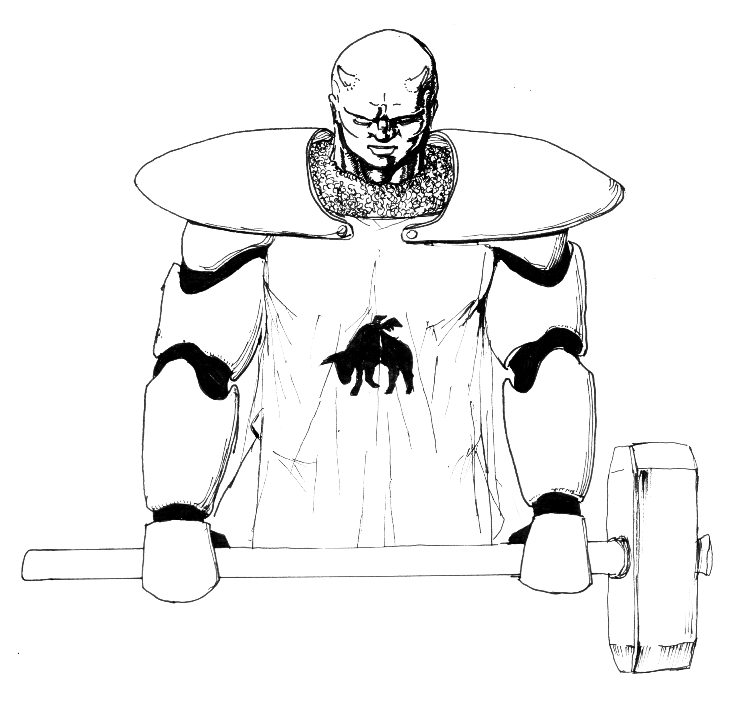
\includegraphics{baystbig.eps}
\end{center}
\end{figure*}

Bayst \`e capace di trasformarsi a piacimento in un enorme toro
bianco la cui cornata infligge 2d8 PV/PSC di danno. Come un toro, non
si cura degli ostacoli che si frappongono tra lui e la sua meta;
infatti la sua tattica prediletta di battaglia consiste nel caricare
gli avversari.

In forma umana combatte utilizzando un Martello da Guerra.
Allorch\'e viene privato di tale arma attacca con pugni e calci. Le
sue abilita di combattimento hanno un TOT pari all'AGI.

I Bayst possono attivare i poteri di: Eutanasia I, Filtro II, Infondi
Vita, Purificazione, Sfera di Immunit\`a, Trasferimento Vitale. 

\carmostro{13+1d10}{14+1d6}{20+1d10}{20+1d10}{20+1d10}{15+1d10}{12+1d10}{150}

\begin{parmostro}{Abilit\`a di Combattimento/TOT/Danno}
\item CAC/AGI/Danno normale
\item ABL/AGI/Danno normale
\end{parmostro}

\begin{parmostro}{Attacchi Particolari/TOT/Danno}
\item Corna/AGI/2d8
\end{parmostro}

\begin{parmostro}{Maestrie/TOT/BON}
\item Martello da Guerra/AGI
\end{parmostro}

\begin{parmostro}{Tecniche Speciali/TOT/BON}
\item Carica/1+BON AGI
\end{parmostro}

\begin{parmostro}{Difese}
\item  Armatura d'avorio (5 PP)
\end{parmostro}

\begin{parmostro}{Poteri Speciali}
\item Eutanasia I
\item Filtro II
\item Infondi Vita
\item Purificazione
\item Sfera di Immunit\`a
\item Trasferimento Vitale
\end{parmostro}

\begin{figure*}[t]
\begin{center}
{\it Johaim}\par\bigskip
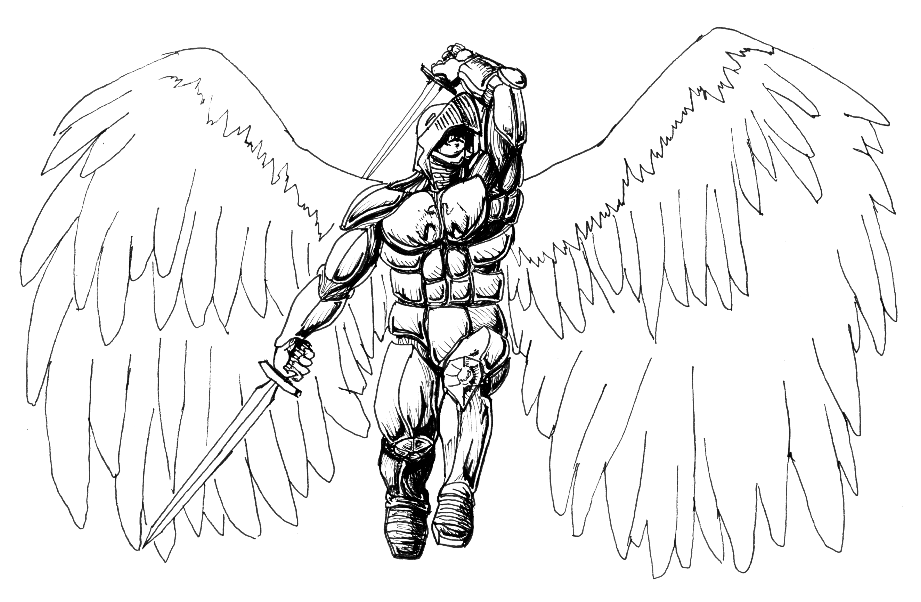
\includegraphics{johaim.eps}
\end{center}
\end{figure*}


\angelo{Johaim}{15}{Quarto Cielo}{Richiamabile}

Appare come un guerriero in armatura di bronzo con una protezione pari
a PP 8, con un elmo a forma di testa d'aquila che non toglie mai.

\`E provvisto di una coppia di ali d'argento che presentano margini
taglienti con le quali pu\`o attaccare ed infliggere 3d8 PV/PSC di
Danno.

Sulla sua armatura \`e raffigurata in bassorilievo un'aquila
d'argento.

Johaim pu\`o tramutarsi in un'aquila di bronzo il cui capo \`e
sormontato da una corona.

Nella forma umana impugna una spada in entrambe le mani. La sua
tattica preferita consiste nel librarsi in volo e attaccare da una
posizione sopraelevata. Le abilit\`a di combattimento hanno un TOT
pari alla sua AGI.

La voce risuona direttamente nella mente del suo interlocutore.

\`E in grado di attivare i poteri di: Eutanasia I, Evoca Angeli I,
Filtro II, Para Urti I, Resurrezione I, Riposo, Risveglio II, Sfera di
vita, Trasferimento Vitale

\carmostro{13+1d10}{14+1d6}{15+1d10}{20+1d10}{13+1d10}{14+1d8}{-}{180}

\begin{parmostro}{Abilit\`a di Combattimento/TOT/Danno}
\item CAC/AGI/Danno normale
\item ATL/AGI/Danno normale
\end{parmostro}

\begin{parmostro}{Attacchi Particolari/TOT/Danno}
\item Ali/AGI/3d8
\end{parmostro}

\begin{parmostro}{Maestrie/TOT/BON}
\item  Spada/AGI
\end{parmostro}

\begin{parmostro}{Tecniche di AM/TOT/BON}
\item Azioni multiple/20/+5
\end{parmostro}

\begin{parmostro}{Difese}
\item Armatura di bronzo (8 PP)
\end{parmostro}

\begin{parmostro}{Poteri speciali}
\item Eutanasia I
\item Evoca Angeli I
\item Filtro II
\item Para Urti I
\item Resurrezione I
\item Riposo
\item Risveglio II
\item Sfera di vita
\item Trasferimento Vitale
\end{parmostro}

\angelo{Custodi Maggiori}{19}{Quarto Cielo}{Richiamabili}

Hanno l'aspetto di uomini, elfi, gnomi, nani o qualsiasi altra razza,
circondati da una brillante luce azzurra che ne mette in risalto i
particolari somatici.  

Vestono le pi\`u svariate armature, dal cuoio
alle piastre e usano armi di qualunque tipo, di cui conoscono la
relativa Abilit\`a di Combattimento ad un TOT pari alla loro AGI.

Possono inoltre servirsi dei poteri di Cura III, DeviaColpo II,
Eutanasia I, Grandezza, Infondi Vita, Para Urti II, Resurrezione II,
Ricostruzione, Sfera di vita, Trasferimento Vitale. 

\carmostro{15+1d10}{14+1d8}{15+2d6}{20+1d10}{15+1d10}{14+1d8}{8+2d6}{225}

\begin{parmostro}{Abilit\`a di Combattimento/TOT/Danno}
\item CAC/AGI/Danno normale
\item ATL o ABL ecc./AGI/Danno normale
\end{parmostro}

\begin{parmostro}{Difese}
\item Armatura (1d8+2 PP)
\end{parmostro}

\begin{parmostro}{Poteri speciali}
\item Cura III
\item Devia Colpo II
\item Eutanasia I
\item Grandezza
\item Infondi Vita
\item Para Urti II
\item Resurrezione II
\item Ricostruzione
\item Sfera di vita
\item Trasferimento Vitale
\end{parmostro}

\angelo{Adonai}{20}{Terzo Cielo}{Richiamabile}

La sua forma \`e quella di un vecchio alto e robusto con i capelli e
la barba candidi e luminosi, che indossa un drappo bianco finemente
decorato. Sulla sua veste, \`e rappresentato un triangolo equilatero
con un occhio al centro.

L'unico punto vitale del suo corpo \`e il torace, che \`e protetto
dal triangolo (10 PP). La mutilazione di una qualunque altra parte del
suo corpo non ne determina la morte.

La sua voce \`e pari al rombo di un tuono; ci\`o implica la
realizzazione di un TR a difficolt\`a 25 per evitare di restare
storditi per il round in corso e quello successivo.

\pinup{adonai.eps}{Adonai}

Adonai combatte con CAC utilizzando in particolare Prese e Proiezioni
con un TOT pari alla sua AGI. La sua tattica preferita \`e quella di
bloccare l'avversario in un abbraccio e successivamente urlargli
contro.

\'E in grado di utilizzare i seguenti poteri: Cura III, Eutanasia II,
Guarigione III, Medicina, Para Urti II, Resurrezione II, Sfera di
Vita.

\carmostro{17+1d8}{16+1d8}{18+1d10}{20+1d10}{18+1d10}{17+1d8}{8+2d6}{240}

\begin{parmostro}{Abilit\`a di Combattimento/TOT/Danno}
\item CAC/AGI/Danno normale
\end{parmostro}

\begin{parmostro}{Attacchi Particolari/TOT/Danno}
\item Voce/TR a 25/Stordimento
\end{parmostro}

\begin{parmostro}{Specifiche di AM/TOT/BON}
\item Presa/AGI/BON Presa
\item  Proiezione/AGI/BON Proiezione
\end{parmostro}

\begin{parmostro}{Difese}
\item Triangolo (10 PP)
\end{parmostro}

\begin{parmostro}{Poteri Speciali}
\item Cura III
\item Eutanasia II
\item Guarigione III
\item Medicina
\item Para Urti II
\item Resurrezione II
\item Sfera di Vita
\end{parmostro}

\angelo{Uziel}{23}{Terzo Cielo}{Richiamabile} 

Ha l'aspetto di un giovane biondo e con i capelli lunghi, dai
lineamenti delicatissimi ed ambigui. Indossa un'armatura d'argento,
capace di proteggerlo con 10 PP, su cui \`e raffigurato un roveto
ardente.\`E dotato di due ali bianche simili a quelle delle colombe.

I suoi occhi brillano di una luce fiammeggiante, pertanto in chiunque
lo guardi in viso induce cecit\`a per 1d4+2 round se non si realizza
un TR a difficolt\`a 30, la voce ricorda un crepitare di fiamme.

Il suo elmo \`e dotato di una celata che abbassa alla bisogna.
Quando la celata \`e abbassata non \`e in grado di provocare la
cecit\`a. 

\`E fornito di un Arco Elfico e di un'Alabarda, che sa
usare alla perfezione. Solitamente si erge in volo ad una certa
distanza dall'avversario e inizia ad attaccare con l'arco. Se privato
delle armi, utilizza i calci. Utilizza l'alabarda anche per effettuare
una micidiale carica in picchiata. La carica ha bisogno di un round di
preparazione.

Le sue abilita di combattimento hanno un TOT pari all'AGI.

Pu\`o usare i poteri di: Devia Colpo II, Eutanasia II, Evoca Angeli I, Evoca
Angeli II, GuarigioneIII, Ibernazione, Incarnazione, Para Urti II, Raggio di
Luce, Resurrezione II. 

\carmostro{17+1d8}{16+1d8}{18+1d10}{20+1d10}{18+1d10}{17+1d8}{19+1d6}{260}

\begin{parmostro}{Abilit\`a di Combattimento/TOT/Danno}
\item CAC/AGI/Danno normale
\item ADT/AGI/Danno normale
\item AIA/AGI/Danno normale
\end{parmostro}

\begin{parmostro}{Attacchi Particolari/TOT/Danno}
\item Cecit\`a/TR a 30/Cecit\`a per 1d4
  round
\end{parmostro}

\begin{parmostro}{Maestrie/TOT/BON}
\item Alabarda/AGI 
\item Arco Elfico/AGI  
\end{parmostro}

\begin{parmostro}{Specifiche di AM/TOT/BON}
\item Calcio/AGI/BON Calcio
\end{parmostro}

\begin{parmostro}{Tecniche Speciali/TOT/BON}
\item Carica/AGI/BON Carica
\end{parmostro}

\begin{parmostro}{Difese}
\item Armatura d'argento (10 PP)
\end{parmostro}

\begin{parmostro}{Poteri speciali}
\item Devia Colpo II
\item Eutanasia II
\item Evoca Angeli I Evoca Angeli II
\item Guarigione III
\item Ibernazione
\item Incarnazione
\item Para Urti II
\item Raggio di Luce
\item Resurrezione II
\end{parmostro}

\angelo{Mikael}{$>$ 30}{Secondo Cielo}{Non Richiamabile}

Appare come un umano alto 2.5 metri, che indossa un'armatura dorata
su cui \`e incisa in bassorilievo una bilancia. Il suo volto pallido \`e
solcato da numerose rughe. 

I suoi occhi sono azzurri e i suoi lunghi capelli
neri sono mossi costantemente da una brezza leggera. \`E dotato di tre coppie
di ali. La sua voce \`e atona e il suo volto non tradisce alcun sentimento.

\angelo{Raphael}{$>$ 30}{Secondo Cielo}{Non Richiamabile} 

Appare come un giovane alto 2 metri e mezzo. I suoi capelli castani
sono lunghi e ricci e gli occhi sono verdi. Indossa, sopra ad una
veste rossa da pellegrino, un'armatura d'oro su cui \`e
raffigurato in bassorilievo un pesce. Impugna un lungo bastone.  Il
suo volto non mostra alcun sentimento. 

Possiede anch'egli tre coppie di ali.

\angelo{Gabriel}{$>$ 30}{Secondo Cielo}{Non Richiamabile} 

Appare come un uomo nel pieno della sua forma fisica, alto 2 metri e
mezzo. I suoi capelli biondi e lisci sono tagliati all'altezza della
nuca e i suoi occhi sono neri.

Indossa, sopra un'ampia tunica verde, un'armatura d'oro su cui
\`e cesellato un ramo d'ulivo. Impugna un grande scettro d'oro. Il
suo volto non mostra alcun sentimento. Possiede anch'egli tre coppie
di ali.

\angelo{Lucifer}{$>$ 30}{Primo Cielo}{Non Richiamabile}

\`E l'angelo che sta a capo della gerarchia. Alto un metro e 80,
appare dotato di tre volti ognuno mostrante un differente sentimento.

\`E dotato di quattro braccia e tre coppie di ali dorate. I suoi
capelli sono rossi, lunghi e ricci e gli occhi dorati. Indossa una
veste candida.

Di solito appare seduto su un trono, circondato da una moltitudine di
altri angeli. Rifulge di una luce talmente potente che lo si pu\`o
guardare soltanto per pochi secondi. 

Pu\`o assumere le sembianze di un qualunque essere vivente.

\subsection{Gli Incantesimi}
\label{incesistenza}
%----------------------------------------------------------------------------
\begin{spell}{Amputazione}{Esistenza}{Attacco}{Danno Mirato}
%----------------------------------------------------------------------------
\descrizione{Fa partire una lama luminosa che infligge 6d6 PV/PSC di danno mirato su un target a contatto col mago.}
%% DR DA DT DB MOD PM PF PE TL
\incvalori{28}{36}{5}{30}{1}{28}{9}{36}{4}
\parametro{Danno}{6}{d6}{30}
\parametro{Base TPC}{0}{}{0}
\fineparametri
\gittatanulla
\campo{1}{target}{2}
\duratanulla
\end{spell}
%----------------------------------------------------------------------------
\begin{spell}{Anestesia}{Esistenza}{Controllo}{Comando}
%----------------------------------------------------------------------------
\descrizione{Fa addormentare un target per 11 minuti se questo non realizza un TV a Diff. 15. Dopo la durata il target dorme per 2d6 ore se non viene svegliato.}
%% DR DA DT DB MOD PM PF PE TL
\incvalori{15}{29}{11}{15}{3}{15}{5}{29}{2}
\parametro{Difficolt\`a del TV}{15}{}{15}
\fineparametri
\gittatanulla
\campo{1}{target}{2}
\durata{11 min}{2}
\end{spell}
%----------------------------------------------------------------------------
\begin{spell}{Antidolore}{Esistenza}{Alterazione}{Variazione abilit\`a fisica}
%----------------------------------------------------------------------------
\descrizione{Conferisce al target un bonus di +10 all'abilit\`a Resistenza al Dolore per 3 minuti.}
%% DR DA DT DB MOD PM PF PE TL
\incvalori{16}{29}{18}{10}{1}{16}{5}{29}{2}
\parametro{Variazione abilit\`a}{10}{punti}{10}
\fineparametri
\gittatanulla
\campo{1}{target}{2}
\durata{3 min}{0}
\end{spell}
%----------------------------------------------------------------------------
\begin{spell}{Antishock}{Esistenza}{Controllo}{Variazione PSIche}
%----------------------------------------------------------------------------
\descrizione{Conferisce un bonus di +5 alla Psiche del target per 3 minuti. Il target si deve a trovare al massimo a 4 metri dal mago.}
%% DR DA DT DB MOD PM PF PE TL
\incvalori{4}{18}{10}{5}{3}{4}{1}{18}{1}
\parametro{Variazione caratteristica PSI}{5}{punti}{5}
\fineparametri
\gittata{4}{1}
\campo{1}{target}{2}
\durata{3 min}{0}
\end{spell}
%----------------------------------------------------------------------------
\begin{spell}{Asservimento Angeli I}{Esistenza}{Evocazione}{Controllo}
%----------------------------------------------------------------------------
\descrizione{Consente di controllare un Angelo della potenza massima di 12 per un periodo massimo di 3 minuti. Il mago pu\`o impartirgli ordini se vince un Confronto di TV con esso se \`e un essere errante, o con chi lo controlla, se \`e controllato da qualcuno.}
%% DR DA DT DB MOD PM PF PE TL
\incvalori{17}{29}{14}{12}{3}{17}{5}{29}{2}
\parametro{Potenza della creatura}{12}{}{12}
\fineparametri
\gittata{4}{1}
\campo{1}{target}{2}
\durata{3 min}{0}
\end{spell}
%----------------------------------------------------------------------------
\begin{spell}{Asservimento Angeli II}{Esistenza}{Evocazione}{Controllo}
%----------------------------------------------------------------------------
\descrizione{Consente di controllare un Angelo della potenza massima di 19 per un periodo di 3 minuti. Il mago pu\`o impartirgli ordini se vince un Confronto di TV con esso se \`e un essere errante, o con chi lo controlla se esso \`e gia controllato.}
%% DR DA DT DB MOD PM PF PE TL
\incvalori{24}{36}{14}{19}{3}{24}{8}{36}{4}
\parametro{Potenza della creatura}{19}{}{19}
\fineparametri
\gittata{4}{1}
\campo{1}{target}{2}
\durata{3 min}{0}
\end{spell}
%----------------------------------------------------------------------------
\begin{spell}{Asservimento Angeli III}{Esistenza}{Evocazione}{Controllo}
%----------------------------------------------------------------------------
\descrizione{Consente di controllare un Angelo della potenza massima di 23 per 3 minuti. Il mago pu\`o impartirgli ordini se vince un confronto di TV con esso se \`e un essere errante, o con chi lo domina se l'essere \`e gi\`a controllato.}
%% DR DA DT DB MOD PM PF PE TL
\incvalori{28}{40}{14}{23}{3}{28}{9}{40}{4}
\parametro{Potenza della creatura}{23}{}{23}
\fineparametri
\gittata{4}{1}
\campo{1}{target}{2}
\durata{3 min}{0}
\end{spell}
%----------------------------------------------------------------------------
\begin{spell}{Barella}{Esistenza}{Alterazione}{Spostamento sul piano}
%----------------------------------------------------------------------------
\descrizione{Fa apparire una barella che consente di trasportare un target posto a non pi\`u di 1 metro di distanza e pesante fino a 120 kg e con 100 kg di equipaggiamento alla velocit\`a di 10 km/h. L'incantesimo viene tenuto a concentrazione. Al venir meno della concentrazione l'effetto prosegue per 3 minuti.}
%% DR DA DT DB MOD PM PF PE TL
\incvalori{16}{29}{16}{6}{7}{16}{5}{29}{2}
\parametro{Massa vivente}{120}{kg}{4}
\parametro{Velocit\`a}{10}{km/h}{1}
\parametro{Massa non vivente}{100}{kg}{1}
\fineparametri
\gittata{1}{0}
\campo{1}{target}{2}
\durata{concentrazione+3 min}{5+0}
\end{spell}
%----------------------------------------------------------------------------
\begin{spell}{Bisturi}{Esistenza}{Alterazione}{Modifica Danni anatomia/armi}
%----------------------------------------------------------------------------
\descrizione{Allunga di 10 cm un'unghia del target, rendendola affilatissima e capace di infliggere 1d6 PV/PSC di danno. L'incantesimo perdura a concentrazione, pi\`u 3 minuti.}
%% DR DA DT DB MOD PM PF PE TL
\incvalori{19}{32}{20}{6}{6}{19}{6}{32}{3}
\parametro{Danno}{1}{d6}{5}
\parametro{Massa}{1}{kg}{1}
\fineparametri
\gittata{1}{0}
\campo{1}{m}{1}
\durata{concentrazione+3 min}{5+0}
\end{spell}
%----------------------------------------------------------------------------
\begin{spell}{Coraggio}{Esistenza}{Controllo}{Variazione VOLont\`a}
%----------------------------------------------------------------------------
\descrizione{Conferisce un bonus di +2 alla Volont\`a di un target posto a non pi\`u di un metro dal mago per la durata di tre minuti.}
%% DR DA DT DB MOD PM PF PE TL
\incvalori{19}{33}{19}{12}{2}{19}{6}{33}{3}
\parametro{Variazione caratteristica}{2}{punti}{12}
\fineparametri
\gittata{1}{0}
\campo{1}{target}{2}
\durata{3 min}{0}
\end{spell}
%----------------------------------------------------------------------------
\begin{spell}{Cura follia}{Esistenza}{Difesa}{Cura}
%----------------------------------------------------------------------------
\descrizione{Restituisce ad un target ad una distanza massima di 1 metro 1d6 di Psiche.}
%% DR DA DT DB MOD PM PF PE TL
\incvalori{5}{25}{21}{2}{2}{5}{1}{25}{1}
\parametro{Riparazione}{1}{d6}{2}
\fineparametri
\gittata{1}{0}
\campo{1}{target}{2}
\duratanulla
\end{spell}
%----------------------------------------------------------------------------
\begin{spell}{Cura I}{Esistenza}{Difesa}{Cura}
%----------------------------------------------------------------------------
\descrizione{Cura 1d6 PV/PSC di danno ad 1 target, purch\'e venga toccato dal mago. Delle ferite guarite non resta alcuna traccia.}
%% DR DA DT DB MOD PM PF PE TL
\incvalori{4}{24}{21}{2}{1}{4}{1}{24}{1}
\parametro{Riparazione}{1}{d6}{2}
\fineparametri
\gittatanulla
\campo{1}{target}{2}
\duratanulla
\end{spell}
%----------------------------------------------------------------------------
\begin{spell}{Cura II}{Esistenza}{Difesa}{Cura}
%----------------------------------------------------------------------------
\descrizione{Cura 3d6 PV/PSC di danno a tutti gli esseri che si trovano in un'area di 1 metro di raggio distante fino a 1 metro dall'usufruitore. Delle ferite guarite non resta alcuna traccia.}
%% DR DA DT DB MOD PM PF PE TL
\incvalori{8}{28}{21}{6}{1}{8}{2}{28}{1}
\parametro{Riparazione}{3}{d6}{6}
\fineparametri
\gittata{1}{0}
\campo{1}{m}{1}
\duratanulla
\end{spell}
%----------------------------------------------------------------------------
\begin{spell}{Cura III}{Esistenza}{Difesa}{Cura}
%----------------------------------------------------------------------------
\descrizione{Cura 7d6 PV/PSC di danno a tutti gli esseri che si trovano in un'area di 4 metro di raggio distante fino a 7 metri dall'usufruitore. Delle ferite guarite non resta alcuna traccia.}
%% DR DA DT DB MOD PM PF PE TL
\incvalori{19}{39}{21}{14}{4}{19}{6}{39}{3}
\parametro{Riparazione}{7}{d6}{14}
\fineparametri
\gittata{4}{1}
\campo{3}{m}{3}
\duratanulla
\end{spell}
%----------------------------------------------------------------------------
\begin{spell}{Devia Colpo I}{Esistenza}{Difesa}{Deviazione}
%----------------------------------------------------------------------------
\descrizione{Devia tutti gli attacchi diretti al target per 3 minuti, con Base TPD pari a 10.}
%% DR DA DT DB MOD PM PF PE TL
\incvalori{16}{36}{25}{10}{1}{16}{5}{36}{2}
\parametro{Base TPD}{10}{punti}{10}
\fineparametri
\gittatanulla
\campo{1}{target}{2}
\durata{3 min}{0}
\end{spell}
%----------------------------------------------------------------------------
\begin{spell}{Devia Colpo II}{Esistenza}{Difesa}{Deviazione}
%----------------------------------------------------------------------------
\descrizione{Devia tutti gli attacchi diretti al target per 3 minuti, con Base TPD pari a 20.}
%% DR DA DT DB MOD PM PF PE TL
\incvalori{26}{46}{25}{20}{1}{26}{8}{46}{4}
\parametro{Base TPD}{20}{punti}{20}
\fineparametri
\gittatanulla
\campo{1}{target}{2}
\durata{3 min}{0}
\end{spell}
%----------------------------------------------------------------------------
\begin{spell}{Erboristeria}{Esistenza}{Informazione}{Variazione abilit\`a mentale}
%----------------------------------------------------------------------------
\descrizione{Conferisce al target un bonus di +9 all'abilit\`a Conoscere Piante o +3 all'abilit\`a Alchimia, per 3 minuti.}
%% DR DA DT DB MOD PM PF PE TL
\incvalori{20}{28}{18}{9}{1}{20}{6}{28}{3}
\parametro{Variazione abilit\`a}{9}{punti}{9}
\fineparametri
\gittatanulla
\campo{1}{target}{2}
\durata{3 min}{0}
\end{spell}
%----------------------------------------------------------------------------
\begin{spell}{Eutanasia I}{Esistenza}{Attacco}{Morte}
%----------------------------------------------------------------------------
\descrizione{Offre il conforto della morte dolce ad un target. Se il target non vuole spegnersi dolcemente pu\`o vanificare l'effetto dell'incantesimo realizzando un TR a Diff. 10.}
%% DR DA DT DB MOD PM PF PE TL
\incvalori{21}{29}{18}{10}{1}{21}{7}{29}{3}
\parametro{Difficolt\`a del TR}{10}{}{10}
\fineparametri
\gittatanulla
\campo{1}{target}{2}
\duratanulla
\end{spell}
%----------------------------------------------------------------------------
\begin{spell}{Eutanasia II}{Esistenza}{Attacco}{Morte}
%----------------------------------------------------------------------------
\descrizione{Offre il conforto della morte dolce ad un target. Se il target non vuole spegnersi dolcemente pu\`o vanificare l'effetto dell'incantesimo realizzando un TR a Diff. 20.}
%% DR DA DT DB MOD PM PF PE TL
\incvalori{31}{39}{18}{20}{1}{31}{10}{39}{5}
\parametro{Difficolt\`a del TR}{20}{}{20}
\fineparametri
\gittatanulla
\campo{1}{target}{2}
\duratanulla
\end{spell}
%----------------------------------------------------------------------------
\begin{spell}{Evoca Angeli I}{Esistenza}{Evocazione}{Richiamo}
%----------------------------------------------------------------------------
\descrizione{Evoca un Caduto, un Rugiel o un Custode Minore per 3 minuti. Il mago pu\`o impartirgli ordini se vince un confronto di TV con esso.}
%% DR DA DT DB MOD PM PF PE TL
\incvalori{20}{32}{18}{12}{2}{20}{6}{32}{3}
\parametro{Potenza della creatura}{12}{}{12}
\fineparametri
\gittata{1}{0}
\campo{1}{target}{2}
\durata{3 min}{0}
\end{spell}
%----------------------------------------------------------------------------
\begin{spell}{Evoca Angeli II}{Esistenza}{Evocazione}{Richiamo}
%----------------------------------------------------------------------------
\descrizione{Evoca un Bayst, un Johaim o un Custode Maggiore (o Angeli di potenza inferiore) per 3 minuti. Il mago pu\`o impartirgli ordini se vince un confronto di TV con esso.}
%% DR DA DT DB MOD PM PF PE TL
\incvalori{27}{39}{18}{19}{2}{27}{9}{39}{4}
\parametro{Potenza della creatura}{19}{}{19}
\fineparametri
\gittata{1}{0}
\campo{1}{target}{2}
\durata{3 min}{0}
\end{spell}
%----------------------------------------------------------------------------
\begin{spell}{Evoca Angeli III}{Esistenza}{Evocazione}{Richiamo}
%----------------------------------------------------------------------------
\descrizione{Evoca un Uziel o un Adonai (o un Angelo di potenza inferiore) per 3 minuti. Il mago pu\`o impartirgli ordini se vince un confronto di TV con esso.}
%% DR DA DT DB MOD PM PF PE TL
\incvalori{31}{43}{18}{23}{2}{31}{10}{43}{5}
\parametro{Potenza della creatura}{23}{}{23}
\fineparametri
\gittata{1}{0}
\campo{1}{target}{2}
\durata{3 min}{0}
\end{spell}
%----------------------------------------------------------------------------
\begin{spell}{Filtro I}{Esistenza}{Difesa}{Scudo antidinamico}
%----------------------------------------------------------------------------
\descrizione{Crea un filtro di luce azzurra che rallenta tutti gli attacchi fisici o quelli magici di danno mirato diretti al target dividendone il danno per 2. L'incantesimo dura 3 minuti.}
%% DR DA DT DB MOD PM PF PE TL
\incvalori{12}{32}{21}{10}{1}{12}{4}{32}{2}
\parametro{Divisore}{2}{unit\`a}{10}
\fineparametri
\gittatanulla
\campo{1}{target}{2}
\durata{3 min}{0}
\end{spell}
%----------------------------------------------------------------------------
\begin{spell}{Filtro II}{Esistenza}{Difesa}{Scudo antidinamico}
%----------------------------------------------------------------------------
\descrizione{Crea un filtro di luce bianca che rallenta tutti gli attacchi fisici o quelli magici di danno mirato diretti al target dividendone il danno per 4. L'incantesimo dura 3 minuti.}
%% DR DA DT DB MOD PM PF PE TL
\incvalori{22}{42}{21}{20}{1}{22}{7}{42}{3}
\parametro{Divisore}{4}{unit\`a}{20}
\fineparametri
\gittatanulla
\campo{1}{target}{2}
\durata{3 min}{0}
\end{spell}
%----------------------------------------------------------------------------
\begin{spell}{Grandezza}{Esistenza}{Alterazione}{Variazione dimensioni}
%----------------------------------------------------------------------------
\descrizione{Dimezza o raddoppia le dimensioni di un target, posto a contatto col mago, pesante fino a 90 kg e che trasporti un equipaggiamento pesante fino a 100 kg. Il target pu\`o opporsi all'incantesimo realizzando un TR a Diff. 18. Dopo 3 minuti il target riprende le sue dimensioni normali.}
%% DR DA DT DB MOD PM PF PE TL
\incvalori{13}{26}{17}{8}{1}{13}{4}{26}{2}
\parametro{Massa vivente}{90}{kg}{3}
\parametro{Massa non vivente}{100}{kg}{1}
\parametro{Fattore dimensione}{2}{unit\`a}{4}
\fineparametri
\gittatanulla
\campo{1}{target}{2}
\durata{3 min}{0}
\end{spell}
%----------------------------------------------------------------------------
\begin{spell}{Guarigione I}{Esistenza}{Difesa}{Resurrezione}
%----------------------------------------------------------------------------
\descrizione{Guarisce in 1d6 giorni un target da una malattia mortale, se la somma del lancio di 5d6 supera il numero di PV originari del target (COSx3 + BON FOR escludendo le variazioni dovute a droghe, incantesimi, etc...) .}
%% DR DA DT DB MOD PM PF PE TL
\incvalori{9}{29}{21}{10}{-2}{9}{3}{29}{1}
\parametro{Riparazione}{5}{d6}{10}
\parametro{Tempo trascorso dalla morte}{0}{giorni}{0}
\fineparametri
\gittatanulla
\campo{1}{target}{2}
\durata{3 min}{0}
\azionetempo{1d6 giorni}{-3}
\end{spell}
%----------------------------------------------------------------------------
\begin{spell}{Guarigione II}{Esistenza}{Difesa}{Resurrezione}
%----------------------------------------------------------------------------
\descrizione{Guarisce in 1d6 giorni da una malattia mortale tutti gli esseri che si trovano in un'area di 3 metri di raggio con centro sul guaritore, se la somma del lancio di 10d6 supera il numero di PV originari dei target (COSx3 + BON FOR escludendo le variazioni dovute a droghe, incantesimi, etc...).}
%% DR DA DT DB MOD PM PF PE TL
\incvalori{20}{40}{21}{20}{-1}{20}{6}{40}{3}
\parametro{Riparazione}{10}{d6}{20}
\parametro{Tempo trascorso dalla morte}{0}{giorni}{0}
\fineparametri
\gittatanulla
\campo{3}{m}{3}
\duratanulla
\azionetempo{1d6 giorni}{-3}
\end{spell}
%----------------------------------------------------------------------------
\begin{spell}{Guarigione III}{Esistenza}{Difesa}{Resurrezione}
%----------------------------------------------------------------------------
\descrizione{Guarisce in 1d6 giorni da una malattia mortale tutti gli esseri che si trovano in un'area di 3 metri di raggio con centro sul guaritore, se la somma del lancio di 15d6 supera il numero di PV originari del target (COSx3 + BON FOR escludendo le variazioni dovute a droghe, incantesimi, etc...) .}
%% DR DA DT DB MOD PM PF PE TL
\incvalori{30}{50}{21}{30}{-1}{30}{10}{50}{5}
\parametro{Riparazione}{15}{d6}{30}
\parametro{Tempo trascorso dalla morte}{0}{giorni}{0}
\fineparametri
\gittatanulla
\campo{3}{m}{3}
\duratanulla
\azionetempo{1d6 giorni}{-3}
\end{spell}
%----------------------------------------------------------------------------
\begin{spell}{Ibernazione}{Esistenza}{Alterazione}{Variazione propriet\`a fisiche}
%----------------------------------------------------------------------------
\descrizione{Conserva permanentemente un corpo di massimo 120 kg di peso, abbassandone la temperatura interna. Pu\`o essere usato anche per conservare cadaveri o cibarie.}
%% DR DA DT DB MOD PM PF PE TL
\incvalori{34}{47}{15}{16}{16}{34}{11}{47}{5}
\parametro{Complessit\`a}{12}{}{12}
\parametro{Massa vivente}{120}{kg}{4}
\parametro{Massa non vivente}{0}{kg}{0}
\fineparametri
\gittatanulla
\campo{1}{target}{2}
\durata{permanente }{15}
\end{spell}
%----------------------------------------------------------------------------
\begin{spell}{Implanto}{Esistenza}{Alterazione}{Modifica Anatomia per nuove funzioni}
%----------------------------------------------------------------------------
\descrizione{Crea un secondo organo per coadiuvare le funzioni di un organo esistente, per 15 minuti.}
%% DR DA DT DB MOD PM PF PE TL
\incvalori{17}{30}{15}{11}{4}{17}{5}{30}{2}
\parametro{Complessit\`a}{10}{}{10}
\parametro{Massa vivente}{30}{kg}{1}
\parametro{Fattore dimensione}{0}{unit\`a}{0}
\fineparametri
\gittatanulla
\campo{1}{target}{2}
\durata{15 min}{3}
\end{spell}
%----------------------------------------------------------------------------
\begin{spell}{Incarnazione}{Esistenza}{Controllo}{Possessione}
%----------------------------------------------------------------------------
\descrizione{Come Trasferimento Vitale, ma l'usufruitore si incarna definitivamente nel corpo del target, fino allo scioglimento dell'incantesimo. Alla morte del corpo originario del mago, l'incantesimo non potr\`a pi\`u essere sciolto.}
%% DR DA DT DB MOD PM PF PE TL
\incvalori{33}{47}{11}{20}{16}{33}{11}{47}{5}
\parametro{Difficolt\`a del TV}{20}{}{20}
\fineparametri
\gittatanulla
\campo{1}{target}{2}
\durata{permanente }{15}
\end{spell}
%----------------------------------------------------------------------------
\begin{spell}{Infondi vita}{Esistenza}{Alterazione}{Creazione Esseri Viventi}
%----------------------------------------------------------------------------
\descrizione{Dona la vita a tutti gli oggetti inanimati inclusi in un'area di 1 metro di raggio, di piccole dimensioni, fino a 30 kg di massa totale (sassi, tavolini, suppellettili) conferendo loro un numero massimo di PCAT di 40. L'incantesimo infonde la vita in 1d6 giorni.}
%% DR DA DT DB MOD PM PF PE TL
\incvalori{24}{37}{29}{11}{-3}{24}{8}{37}{4}
\parametro{Massa vivente}{30}{kg}{1}
\parametro{punti CAraTteristica}{40}{punti}{10}
\fineparametri
\gittatanulla
\campo{1}{m}{1}
\duratanulla
\azionetempo{1d6 giorni}{-3}
\end{spell}
%----------------------------------------------------------------------------
\begin{spell}{Medicina}{Esistenza}{Informazione}{Variazione abilit\`a mentale}
%----------------------------------------------------------------------------
\descrizione{Attribuisce al target un bonus di +5 all'abilit\`a Medicina per 15 minuti.}
%% DR DA DT DB MOD PM PF PE TL
\incvalori{29}{37}{18}{15}{4}{29}{9}{37}{4}
\parametro{Variazione abilit\`a}{15}{punti}{15}
\fineparametri
\gittatanulla
\campo{1}{target}{2}
\durata{15 min}{3}
\end{spell}
%----------------------------------------------------------------------------
\begin{spell}{Para Urti I}{Esistenza}{Difesa}{Parata}
%----------------------------------------------------------------------------
\descrizione{Crea due sfere luminose orbitanti attorno al target aventi lo scopo di parare ciascuna un attacco diretto ad esso, con Base TPD pari a 20. Ognuna delle sfere scompare dopo aver parato un attacco. Le sfere scompaiono comunque dopo 3 minuti.}
%% DR DA DT DB MOD PM PF PE TL
\incvalori{20}{40}{15}{24}{1}{20}{6}{40}{3}
\parametro{Base TPD}{20}{punti}{20}
\parametro{Parate}{2}{}{4}
\fineparametri
\gittatanulla
\campo{1}{target}{2}
\durata{3 min}{0}
\end{spell}
%----------------------------------------------------------------------------
\begin{spell}{Para Urti II}{Esistenza}{Difesa}{Parata}
%----------------------------------------------------------------------------
\descrizione{Crea 5 sfere luminose orbitanti attorno al target aventi lo scopo di parare ciascuna un attacco diretto ad esso, con Base TPD pari a 20. Ognuna delle sfere scompare dopo aver parato un attacco. Le sfere scompaiono comunque dopo 3 minuti.}
%% DR DA DT DB MOD PM PF PE TL
\incvalori{26}{46}{15}{30}{1}{26}{8}{46}{4}
\parametro{Base TPD}{20}{punti}{20}
\parametro{Parate}{5}{}{10}
\fineparametri
\gittatanulla
\campo{1}{target}{2}
\durata{3 min}{0}
\end{spell}
%----------------------------------------------------------------------------
\begin{spell}{Protezione Angeli I}{Esistenza}{Evocazione}{Protezione}
%----------------------------------------------------------------------------
\descrizione{Viene creata attorno al mago un'area di 3 metri di raggio all'interno della quale gli angeli di potenza inferiore o uguale a 12 non possono entrare se non realizzando un TV a Diff. 22. Realizzando un TV le creature potranno avanzare di 1 metro, subendo 1d6 PV di danno netto per ogni metro all'interno dell'area, L'incantesimo scompare se un essere all'interno dell'area protetta attacca le creature dalle quali si sta proteggendo. Per ogni metro all'interno dell'area il TV delle creature \`e penalizzato di -1. L'incantesimo perdura per 3 minuti.}
%% DR DA DT DB MOD PM PF PE TL
\incvalori{12}{24}{10}{12}{2}{12}{4}{24}{2}
\parametro{Potenza della creatura}{12}{}{12}
\fineparametri
\gittatanulla
\campo{3}{m}{3}
\durata{3 min}{0}
\end{spell}
%----------------------------------------------------------------------------
\begin{spell}{Protezione Angeli II}{Esistenza}{Evocazione}{Protezione}
%----------------------------------------------------------------------------
\descrizione{Viene creata attorno al mago un'area di 3 metri di raggio all'interno della quale gli angeli di potenza inferiore o uguale a 19 non possono entrare se non realizzando un TV a Diff. 29 Realizzando un TV le creature potranno avanzare di 1 metro, subendo 1d6 PV di danno netto per ogni metro all'interno dell'area, L'incantesimo scompare se un essere all'interno dell'area protetta attacca le creature dalle quali si sta proteggendo. Per ogni metro all'interno dell'area il TV delle creature \`e penalizzato di -1. L'incantesimo perdura per 3 minuti.}
%% DR DA DT DB MOD PM PF PE TL
\incvalori{19}{31}{10}{19}{2}{19}{6}{31}{3}
\parametro{Potenza della creatura}{19}{}{19}
\fineparametri
\gittatanulla
\campo{3}{m}{3}
\durata{3 min}{0}
\end{spell}
%----------------------------------------------------------------------------
\begin{spell}{Protezione Angeli III}{Esistenza}{Evocazione}{Protezione}
%----------------------------------------------------------------------------
\descrizione{Viene creata attorno al mago un'area di 3 metri di raggio all'interno della quale gli angeli di potenza inferiore o uguale a 23 non possono entrare se non realizzando un TV a Diff. 33. Realizzando un TV le creature potranno avanzare di 1 metro, subendo 1d6 PV di danno netto per ogni metro all'interno dell'area, L'incantesimo scompare se un essere all'interno dell'area protetta attacca le creature dalle quali si sta proteggendo. Per ogni metro all'interno dell'area il TV delle creature \`e penalizzato di -1. L'incantesimo perdura per 3 minuti.}
%% DR DA DT DB MOD PM PF PE TL
\incvalori{23}{35}{10}{23}{2}{23}{7}{35}{3}
\parametro{Potenza della creatura}{23}{}{23}
\fineparametri
\gittatanulla
\campo{3}{m}{3}
\durata{3 min}{0}
\end{spell}
%----------------------------------------------------------------------------
\begin{spell}{Purificazione}{Esistenza}{Alterazione}{Variazione propriet\`a fisiche}
%----------------------------------------------------------------------------
\descrizione{Sterilizza cibo e acqua fino ad una massa totale di 100 kg. Se il cibo purificato non viene conservato in maniera idonea entro 3 minuti, potr\`a nuovamente andare a male.}
%% DR DA DT DB MOD PM PF PE TL
\incvalori{9}{22}{15}{7}{0}{9}{3}{22}{1}
\parametro{Complessit\`a}{6}{}{6}
\parametro{Massa vivente}{0}{kg}{0}
\parametro{Massa non vivente}{100}{kg}{1}
\fineparametri
\gittatanulla
\campo{1}{m}{1}
\durata{3 min}{0}
\end{spell}
%----------------------------------------------------------------------------
\begin{spell}{Raggio di luce}{Esistenza}{Attacco}{Danno Netto}
%----------------------------------------------------------------------------
\descrizione{Investe un target di un lampo luminoso di energia che gli infligge 10d6 PV (Pi\`u eventuali Danni Addizionali da ustione) di danno netto dimezzabile con un TR a Diff. 30. L'incantesimo deve essere effettuato a contatto.}
%% DR DA DT DB MOD PM PF PE TL
\incvalori{34}{42}{21}{20}{1}{34}{11}{42}{5}
\parametro{Danno}{10}{d6}{20}
\fineparametri
\gittatanulla
\campo{1}{target}{2}
\duratanulla
\end{spell}
%----------------------------------------------------------------------------
\begin{spell}{Restauro}{Esistenza}{Difesa}{Riparazione danni}
%----------------------------------------------------------------------------
\descrizione{Ripara danni a tutti gli oggetti posti all'interno di un'area di 3 metri di raggio, per un totale di 5d6 Punti Struttura per ogni oggetto. Il centro dell'area di 3 metri pu\`o distare fino ad 1 metro dal mago.}
%% DR DA DT DB MOD PM PF PE TL
\incvalori{8}{28}{15}{10}{3}{8}{2}{28}{1}
\parametro{Riparazione}{5}{d6}{10}
\fineparametri
\gittata{1}{0}
\campo{3}{m}{3}
\duratanulla
\end{spell}
%----------------------------------------------------------------------------
\begin{spell}{Resurrezione I}{Esistenza}{Difesa}{Resurrezione}
%----------------------------------------------------------------------------
\descrizione{Resuscita un target se il risultato del lancio di 7d6 supera o eguaglia il numero totale dei PV originari del target (COSx3 + BON FOR escludendo gli effetti di droghe, incantesimi, etc...), purch\'e non sia trascorso pi\`u di 1 giorno dal decesso.}
%% DR DA DT DB MOD PM PF PE TL
\incvalori{17}{37}{21}{15}{1}{17}{5}{37}{2}
\parametro{Riparazione}{7}{d6}{14}
\parametro{Tempo trascorso dalla morte}{1}{giorno}{1}
\fineparametri
\gittatanulla
\campo{1}{target}{2}
\durata{3 min}{0}
\end{spell}
%----------------------------------------------------------------------------
\begin{spell}{Resurrezione II}{Esistenza}{Difesa}{Resurrezione}
%----------------------------------------------------------------------------
\descrizione{Resuscita un target se il risultato del lancio di 10d6 supera o eguaglia il numero totale dei PV originari del target (COSx3 + BON FOR escludendo gli effetti di droghe, incantesimi, etc...), purch\'e non siano trascorsi pi\`u di 5 giorni dal decesso.}
%% DR DA DT DB MOD PM PF PE TL
\incvalori{27}{47}{21}{25}{1}{27}{9}{47}{4}
\parametro{Riparazione}{10}{d6}{20}
\parametro{Tempo trascorso dalla morte}{5}{giorni}{5}
\fineparametri
\gittatanulla
\campo{1}{target}{2}
\durata{3 min}{0}
\end{spell}
%----------------------------------------------------------------------------
\begin{spell}{Ricostruzione}{Esistenza}{Difesa}{Riparazione danni}
%----------------------------------------------------------------------------
\descrizione{Ripara danni a tutti gli oggetti posti all'interno di un'area di 10 metri di raggio, per un totale di 10d6 Punti Struttura per ogni oggetto. Il centro dell'area di 10 metri pu\`o distare fino a 4 metri dal mago. I danni verranno riparati gradualmente in 1d6 giorni.}
%% DR DA DT DB MOD PM PF PE TL
\incvalori{23}{43}{15}{20}{8}{23}{7}{43}{3}
\parametro{Riparazione}{10}{d6}{20}
\fineparametri
\gittata{4}{1}
\campo{10}{m}{10}
\durata{3 min}{0}
\azionetempo{1d6 giorni}{-3}
\end{spell}
%----------------------------------------------------------------------------
\begin{spell}{Riposo}{Esistenza}{Difesa}{Cura}
%----------------------------------------------------------------------------
\descrizione{Restituisce al target 4d6 PF o 4d6 PM.}
%% DR DA DT DB MOD PM PF PE TL
\incvalori{10}{30}{21}{8}{1}{10}{3}{30}{1}
\parametro{Riparazione}{4}{d6}{8}
\fineparametri
\gittatanulla
\campo{1}{target}{2}
\duratanulla
\end{spell}
%----------------------------------------------------------------------------
\begin{spell}{Risveglio I}{Esistenza}{Difesa}{Rianimazione}
%----------------------------------------------------------------------------
\descrizione{Rianima dal coma un target se il risultato del lancio di 5d6 eguaglia o supera il numero totale dei PV originari del target (COSx3 + BON FOR escludendo gli effetti di droghe, incantesimi, etc...).}
%% DR DA DT DB MOD PM PF PE TL
\incvalori{6}{26}{15}{10}{1}{6}{2}{26}{1}
\parametro{Riparazione}{5}{d6}{10}
\fineparametri
\gittatanulla
\campo{1}{target}{2}
\duratanulla
\end{spell}
%----------------------------------------------------------------------------
\begin{spell}{Risveglio II}{Esistenza}{Difesa}{Rianimazione}
%----------------------------------------------------------------------------
\descrizione{Rianima dal coma un target se il risultato del lancio di 10d6 eguaglia o supera il numero totale dei PV originari del target (COSx3 + BON FOR escludendo gli effetti di droghe, incantesimi, etc...).}
%% DR DA DT DB MOD PM PF PE TL
\incvalori{16}{36}{15}{20}{1}{16}{5}{36}{2}
\parametro{Riparazione}{10}{d6}{20}
\fineparametri
\gittatanulla
\campo{1}{target}{2}
\duratanulla
\end{spell}
%----------------------------------------------------------------------------
\begin{spell}{Sfera di immunit\`a}{Esistenza}{Difesa}{Protezione Magica}
%----------------------------------------------------------------------------
\descrizione{Protegge tutti i target che stanno all'interno di un'area di 1 metro di raggio, distante fino a 1 metro dall'usufruitore, da ogni incantesimo di Attacco/Danno netto, assorbendo 7d6 di danno, nel corso di 3 minuti.}
%% DR DA DT DB MOD PM PF PE TL
\incvalori{15}{35}{20}{14}{1}{15}{5}{35}{2}
\parametro{Protezione}{7}{d6}{14}
\fineparametri
\gittata{1}{0}
\campo{1}{m}{1}
\durata{3 min}{0}
\end{spell}
%----------------------------------------------------------------------------
\begin{spell}{Sfera di vita}{Esistenza}{Difesa}{Armatura}
%----------------------------------------------------------------------------
\descrizione{Crea una sfera di 1 metro di raggio che garantisce una protezione pari a 10 PP a tutti coloro che stanno al suo interno. La protezione dura 3 minuti.}
%% DR DA DT DB MOD PM PF PE TL
\incvalori{20}{40}{19}{20}{1}{20}{6}{40}{3}
\parametro{Protezione}{10}{PP}{20}
\fineparametri
\gittata{1}{0}
\campo{1}{m}{1}
\durata{3 min}{0}
\end{spell}
%----------------------------------------------------------------------------
\begin{spell}{Trasferimento vitale}{Esistenza}{Controllo}{Possessione}
%----------------------------------------------------------------------------
\descrizione{L'usufruitore trasferisce la sua essenza vitale all'interno di un ospite per 15 minuti. Durante questo tempo il corpo dell'usufruitore rester\`a in catalessi. Il target potr\`a sottrarsi all'incantesimo realizzando un TV a Diff. 20.}
%% DR DA DT DB MOD PM PF PE TL
\incvalori{21}{35}{11}{20}{4}{21}{7}{35}{3}
\parametro{Difficolt\`a del TV}{20}{}{20}
\fineparametri
\gittatanulla
\campo{1}{target}{2}
\durata{15 min}{3}
\end{spell}



%%---------------------------------------------------------------------------
\vfill\section{Illusionismo}
%%---------------------------------------------------------------------------

\Simbolo{simb_ill.eps}

L'altra parte del regno Memath,  l'Illusionismo, o Magia dell'Illusione
in Novese o Via del Pensiero in Elfico, presiede i poteri della mente e
dell'inconscio.

Simbolo degli illusionisti sono tre cerchi concentrici con un occhio
aperto stilizzato nel centro.

\subsection{Dominio}

Tutti gli incantesimi degli illusionisti sono legati
ai poteri della mente, e hanno a che fare con i pensieri e i sogni
delle creature. La scuola dell'Illusionismo \`e in contatto magico
con la Dimora Onirica, sede degli Incubi e dei Sogni dei viventi. Le
creature oniriche possono essere richiamate nel mondo reale solo dagli
illusionisti. 

L'esistenza della Dimora Onirica \`e determinata dai
sogni dei vivi. Gli oggetti che vi si trovano non sono permanenti, per
la maggior parte appaiono e scompaiono spesso repentinamente,
cos\`{\i} come i pensieri e i sogni degli uomini. 

Nella Dimora Onirica
qualsiasi oggetto pu\`o essere creato semplicemente desiderandolo e
quasi tutti gli oggetti possono essere distrutti o modificati nello
stesso modo. Esattamente quello che avviene nei sogni. 

Nell'Onirica le creature sono riunite in cinque Dimore in ordine di
potere. Ogni dimora \`e alimentata dagli incubi e dai sogni
dell'et\`a relativa. 

\begin{description} 
\item{\bf La Quinta Dimora} ospita gli incubi e i sogni degli esseri
  pensanti \textbf{adulti} e maturi. Per evocare un essere di V dimora
  \`e necessario che ci sia un dormiente di quell'et\`a a meno di
  1000 metri da chi tenta il richiamo.
  
\item{\bf La Quarta Dimora} ospita gli incubi e i sogni degli esseri
  pensanti che hanno da poco\textbf{ oltrepassato la maturit\`a.}
  Per evocare un essere di IV dimora \`e necessario che ci sia un
  dormiente di quell'et\`a a meno di 1000 metri da chi tenta il
  richiamo.
  
\item{\bf La Terza Dimora} ospita gli incubi e i sogni degli esseri
  pensanti che hanno superato l'infanzia ma non sono ancora giunti
  alla soglia dell'et\`a adulta. Per evocare un essere di III dimora \`e
  necessario che ci sia un dormiente di quell'et\`a a meno di 1000
  metri da chi tenta il richiamo.
  
\item{\bf La Seconda Dimora} ospita gli incubi e i sogni degli esseri
  pensanti dell'et\`a senile. Gli esseri onirici di seconda dimora
  non si possono richiamare, ma talvolta autonomamente oltrepassano il
  confine della dimora onirica per introdursi nel mondo reale.
  
\item{\bf La Prima Dimora} ospita gli incubi e i sogni degli esseri
  pensanti che attraversano l'infanzia. Essa \`e permeata
  dall'essenza del Babau.
\end{description}

\subsection{Limiti e peculiarit\`a}

Solo gli illusionisti possono evocare e controllare le creature
dell'incubo e del sogno. Per evocare un essere onirico della 3$^a${
  d}imora bisogna che, nel raggio di 1 km, un ``adolescente'', di
qualsiasi specie animale, stia sognando. Per evocare un essere onirico
della 4$^a${ d}imora bisogna che, nel raggio di 1 km, un ``anziano''
di qualsiasi specie animale stia sognando. Per evocare un essere
onirico della 5$^a${ d}imora bisogna che, nel raggio di 1 km, un
``adulto'' di qualsiasi specie animale stia sognando.

Solo gli illusionisti sono in grado di proiettare la loro coscienza
all'interno della dimora onirica, e cos\`{\i} influenzare i sogni dei
dormienti. Per fare ci\`o devono effettuare la seguente
``cerimonia'':
\begin{itemize}
\item Realizzare un TCONC a 25
\item Realizzare un tiro sulla scuola di magia Illusionismo a
  difficolt\`a 20
\item Addormentarsi per almeno 30 minuti
\item Realizzare un Confronto di TV con un dormiente, scelto come
  ``porta di accesso'' alla dimora onirica, che si deve trovare a meno
  di 10 metri da loro.
\end{itemize}

Se la ``porta'' si sveglia il contatto consapevole con la dimora
onirica si scioglie. Il mago si pu\`o svegliare a sua volta
realizzando un TCONC a 20. In caso di fallimento del TCONC il mago
continuer\`a a dormire.

In caso di
riuscita il mago potr\`a decidere se svegliarsi o continuare a
dormire. 

Se anche uno solo dei 4 ``passi'' della cerimonia non va a
buon fine, essa non riesce. Il mago potr\`a addormentarsi e
continuare a dormire senza poter influenzare i sogni altrui. Il mago
consumer\`a 1 PE per ogni TV tentato nella Dimora Onirica. Gli
adepti dell'illusionismo infliggono il danno magicamente, mediante
``danni illusori'', ``convincendo'' le vittime degli incantesimi di
aver subito danni. Il danno illusorio toglie PV e PSC esattamente come
il danno reale. 

I Danni Illusori si infliggono come qualsiasi
incantesimo di Attacco.

\subsection{Potenzialit\`a} 
\begin{tabular}{lc}
Evocazione& 14\\
Alterazione& 9 \\
Controllo& 20 \\
Informazione& 16\\
Difesa& 11 \\
Attacco& 5\\
\end{tabular}

\subsection{Leggi dell'uso}
\begin{enumerate}\itemsep -6pt
\item Non lasciare liberi gli esseri onirici
\item Non annullare la volont\`a di un Arcimago 
\end{enumerate}


\subsection{Gli Esseri Onirici}

Gli Esseri Onirici, detti anche Creature Oniriche, si dividono in due
grandi categorie: Incubi e Sogni. 

Gli incubi e i sogni hanno vita e volont\`a proprie e risiedono
perennemente nella dimora onirica, di cui fanno parte e a cui sono
rigidamente legati.

Il loro comportamento \`e illogico e caotico.  Se due creature
oniriche si incontrano, generalmente intraprendono un cruento
combattimento all'ultimo sangue, indipendentemente dalla differenza di
forza tra i due, ma a volte capita che si ignorino o (pi\`u
raramente) che si alleino per uno scopo comune.

In ogni caso per ogni creatura onirica distrutta se ne
rigenera dopo un certo tempo una simile, in modo tale che il numero delle creature
oniriche sia sempre strettamente legato al numero di viventi. 

Tutte queste creature possono assumere nella Dimora Onirica la forma e
l'aspetto che desiderano, comprese le forme geometriche o di oggetti
invisibili, bench\'e ogni specie ne abbia una preferita.

In genere gli incubi sono molto brutti, schifosi o raccapriccianti,
mentre i sogni sono solitamente belli e gradevoli agli occhi dei
sognatori.  I sogni e gli incubi non sentono dolore e sono immuni alle
malattie.

Per sconfiggerli \`e necessario inabilitarli, portare a 0 i loro PV,
distruggere totalmente il corpo o distruggere il punto vitale tipico
della specie. 

Se parti dei loro corpi vengon danneggiate o distrutte durante i
combattimenti, essi perdono i PV e i PSC ed eventualmente le
funzionalit\`a della parte amputata.

\es{Un incubo che ha gli occhi sulla testa viene decapitato. La testa
  non \`e il punto vitale tipico della sua specie, quindi continua
  tranquillamente a muoversi e a combattere (con i malus per la
  perdita dei PV), ma perde la capacit\`a di vedere}

Se vengono ``divisi'' in pi\`u parti, solo una di esse sopravvive.

Una volta ridotti a 0 i loro PV, anche se il loro corpo non \`e
stato totalmente disintegrato, essi scompaiono.

Una volta evocati, gli incubi e i sogni perdono il potere di creare
oggetti, e assumono la forma tipica della loro razza, conservando
per\`o la capacit\`a di alterare gli stati d'animo e l'indole
originaria: gli incubi sono generalmente crudeli, i sogni sono di
indole buona, bench\'e entrambe le classi siano assolutamente
caotiche e imprevedibili. 

I sogni e gli incubi (sia nella loro forma nativa che in quella
concreta che assumono in seguito all'evocazione) hanno sommariamente
poteri dello stesso livello e sono in grado incutere nel sognatore una
sensazione tipica della razza a cui appartengono.

Generalmente gli incubi (da qui il loro nome) tendono a incutere
dolore, paura, terrore o ansia, mentre i sogni si orientano verso una
semplice indifferenza o verso allegria, benessere o piacere.

Sia i sogni che gli incubi sono suddivisi in cinque Dimore, di potenza
crescente dalla quinta alla prima.  

Per evocare una creatura onirica, deve esserci almeno un sognatore
adatto (per et\`a o indole) nel raggio di 1000 metri. La creatura
evocata scompare se tutti i sognatori in tale raggio si svegliano.

Mentre la Diff. di Conoscere un incubo \`e generalmente pari alla sua
Potenza $+10$, la difficolt\`a di conoscere un sogno \`e pari alla sua
Potenza $+15$.

\subsubsection{Le raffigurazioni} 

Le raffigurazioni sono gli esseri od oggetti sognati dai vivi. Possono
essere modificate o distrutte con la volont\`a (in tal caso
scompaiono dal sogno) e create con la stessa.  In entrambi i casi
occorre effettuare un Confronto di TV tra il costruttore e il
distruttore.

Le raffigurazioni possono essere concretizzate. In tal caso vengono
``spostate'' dal sogno al piano materiale e spariscono definitivamente
dal sogno (il sognatore pu\`o comunque ricrearle al sogno
successivo, dopo essersi svegliato). Una raffigurazione \`e solo la
rappresentazione di un oggetto o di una persona, ed \`e pertanto
priva di quasi tutte le funzionalit\`a tipiche.

Una spada concretizzata quindi pu\`o non tagliare (ma pu\`o essere
sempre usata allo scopo di percuotere).  Un uomo (o un essere vivente)
concretizzato pu\`o non pensare o agire per conto proprio, ma
si comporta come un automa, eseguendo gesti stereotipati o
pronunciando frasi ovvie o senza senso.

Una raffigurazione concretizzata non pu\`o avere caratteristiche
superiori a quelle dell'oggetto che rappresenta e pu\`o essere solo
leggermente differente per struttura, dimensioni e proporzioni;
inoltre non pu\`o avere poteri magici di alcun tipo. 

In termini di gioco l'incantesimo di concretizzazione di una
raffigurazione si deve classificare nel tipo ``Alterazione/ Creazione
Oggetti'' o ``Alterazione/ Creazione Esseri Viventi''.

Una raffigurazione, comunque, non pu\`o superare il punteggio di 5
nel TOT per nessuna abilit\`a. 

Un particolare tipo di raffigurazione \`e l'\textbf{alter ego}, ossia
l'idea che un sognatore ha di se stesso nel sogno. Tale raffigurazione
non pu\`o essere evocata n\`e fatta scomparire con un TV e ha
caratteristiche pari a quelle del sognatore, meno 10 (la bellezza non
subisce il malus).

L'alter ego si comporta in un sogno pi\`u o meno come farebbe il
sognatore stesso, bench\'e le azioni compiute siano per lo pi\`u
illogiche e confuse. 

Uccidendo un alter ego il sognatore si sveglia.

Le informazioni raccolte dall'alter ego vengono acquisite dal
sognatore al risveglio se questo realizza un TCONC a 20, in caso
contrario il sognatore dimentica il sogno. 

\incubo{Braak}{5}{Quinta Dimora}{Richiamabile}

Assumono la forma di un grosso sacco azzurro a chiazze gialle,
carnoso, con la parte inferiore coperta di peli bianchi, e la parte
superiore setolosa. Hanno una grande bocca irregolare irta di denti
triangolari affilati e un numero di occhi variabile tra uno e cinque,
tutti disposti in fila orizzontale al di sopra della bocca.

Possiedono due, quattro, cinque o sette braccia (se le braccia sono in
numero dispari, una di esse si incastra sulla sommit\`a della
``testa'') lunghe e sottili, con mani e dita lunghissime, appuntite e
affusolate.

\pinup{braak.eps}{Braak}

Si muovono volando non troppo rapidamente a pochi centimetri da terra
(ma possono raggiungere una quota anche elevata) e raggiungono le
dimensioni di un uomo alto e robusto.  Combattono a mani nude
sfruttando le loro armi naturali: il grosso pugno che pu\`o
infliggere 2d6 PV/PSC di danno; la stretta delle lunghe dita, che
infligge 1d8 PV/PSC di danno, e il morso, che infligge 1d6 PV/PSC di
danno. La superficie del loro corpo \`e coriacea e li protegge per
un valore di 1 PP. Il loro punto vitale \`e il grosso torace.

\carmostro{6+1d6}{4+2d8}{10+2d6}{10+1d6}{10+2d6}{4+3d6}
{3-1d6}{45}

\begin{parmostro}{Abilit\`a di Combattimento/TOT/Danno}
\item CAC/AGI-3/Danno Normale
\end{parmostro}

\begin{parmostro}{Attacchi Particolari/TOT/Danno}
\item Pugno/AGI/2d6
\item Presa/AGI/1d8
\item Morso/AGI-4/1d6
\end{parmostro}

\begin{parmostro}{Difese}
\item Pelle coriacea (PP 1)
\end{parmostro}

\begin{parmostro}{Poteri speciali}
\item Paralisi I
\item Sonno I
\end{parmostro}

\incubo{Greyant}{6}{Quinta  Dimora}{Richiamabile}

Se evocati appaiono come delle formiche grigie lunghe dai due ai
quattro metri.

Hanno due occhi composti di colore arancione debolmente luminosi, che
conferiscono loro un'aspetto spettrale. Il corpo \`e
completamente ricoperto di peli grigi che puzzano di muffa. 

Sulla testa hanno due coppie di mandibole che usano per torturare e
stritolare e sono muniti di otto zampe. Una volta individuato un
bersaglio, lo catturano e non lo abbandonano fino alla sua morte, se
non per una fuga strategica. 

Il loro morso infligge 2d8 PV/PSC di danno. 

Il loro guscio esterno funziona come una armatura, proteggendoli per 5
PP. Se si esclude un fischio raccapricciante, sono completamente muti.
Il loro punto vitale \`e la testa.

\carmostro{4+1d6}{4+2d8}{15+1d10}{4+1d6}{15+1d10}{4+1d6} {-}{60}

\begin{parmostro}{Abilit\`a di combattimento/TOT/Danno}
\item CAC/AGI/Danno Normale
\end{parmostro}

\begin{parmostro}{Attacchi Particolari/TOT/Danno}
\item Morso/AGI-1/2d8 
\end{parmostro}

\begin{parmostro}{Difese}
\item Corazza (PP 5)
\end{parmostro}

\begin{parmostro}{Poteri Speciali}
\item Buio
\item Fetore
\item Paralisi I
\item Paura I
\end{parmostro}

\sogno{Blink}{6}{Quinta Dimora}{Richiamabile}

Si presenta come una lucina puntiforme e multicolore in continuo
movimento.  Si sposta fluttuando lentamente fino a 4 m da terra (o
dall'acqua), \`e capace di effettuare scatti velocissimi fino ad 1
metro (1 scatto per round al massimo) ed \`e in grado di introdursi
in qualunque apertura, compresi gli orifizi corporei. 

La sua forza si manifesta sotto forma di un'onda di pressione sferica
con centro nella lucina e raggio 50 cm, che funziona come una
Proiezione che infligge 2d6 PV/PSC di danno.

Se colpito la sua luce si affievolisce, fino a
spegnersi del tutto alla sua morte. I suoi colpi permessi di CAC sono
limitati a Schivare, Divincolarsi, Caduta. Non ha punti vitali, ma non
\`e molto resistente ai colpi. 

\`E in grado di comunicare esclusivamente con la telepatia ed ha una
tendenza particolare agli scherzi. Suscita divertimento.

\carmostro{10+1d6}{4+2d8}{6+1d6}{10+1d10}{6+1d10}{4+2d8} {-}{75}

\begin{parmostro}{Abilit\`a di Combattimento/TOT/Danno}
\item CAC/AGI/1d4
\end{parmostro}

\begin{parmostro}{Specifiche di AM/TOT/BON}
\item Schivare/20/+5
\end{parmostro}

\begin{parmostro}{Attacchi Particolari/TOT/Danno}
\item Onda di pressione/AGI/2d6
\end{parmostro}

\begin{parmostro}{Poteri speciali}
\item Ilarit\`a 
\item Paralisi I
\item Sonno I
\end{parmostro}



\incubo{Bleargh}{9}{Quarta Dimora}{Richiamabile}

Se evocati appaiono come un ammasso pi\`u o meno informe di tessuti
organici umidicci e puzzolenti, da cui si dipartono diverse appendici
con funzioni differenti: quelle oculari (bulbi oculari peduncolati),
quelle uncinate (ganci ossei, capaci di infliggere 2d6 PV/PSC di
danno) e quelle a ventosa attraverso le quali possono risucchiare la
``forza'' (assorbendo 2d4+1 PF) dei loro avversari.

Le Ventose vengono usate per effettuare Prese. I Bleargh non brandiscono
armi. Si muovono molto rapidamente strisciando o ondeggiando su
pseudopodi o tentacoli. Sono comunque molto sensibili ai colpi e non
hanno una grande forza. Un solo punto del loro corpo a scelta del
Master \`e da considerare ``punto vitale''.

\carmostro{10+1d6}{8+2d6}{6+1d6}{15+1d10}{6+1d6}{10+1d20}
{-1d6}{85} 

\begin{parmostro}{Abilit\`a di combattimento/TOT/Danno}
\item CAC/AGI/Danno Normale
\end{parmostro}

\begin{parmostro}{Attacchi Particolari/TOT/Danno}
\item Uncini/AGI/2d6 
\item Ventosa/AGI-2/2d4+1 PF
\end{parmostro}

\pinup{bleargh.eps}{Bleargh}

\begin{parmostro}{Poteri speciali}
\item Buio
\item Evoca Essere Onirico I
\item Invisibilit\`a
\item Ipnosi I
\item Paralisi I
\item Sonno II
\end{parmostro}

\sogno{Succubi}{9}{Quarta Dimora}{Richiamabile}

Si presentano come esseri bellissimi, nudi, della stessa razza ed
etnia dell'illusionista che li evoca, il quale \`e in grado di
stabilire il loro sesso (eventuale) solo se riesce vincere il
confronto di TV. 

Scopo della loro esistenza \`e quello di causare il piacere sensuale
dei viventi.

Sono molto astuti, agili e veloci nei movimenti ma non sono dotati di
una grande forza. Compensano la loro debolezza con sensi molto
sviluppati e una notevole capacit\`a di seduzione, che costituisce la
loro peculiarit\`a.

Possono risucchiare la forza (assorbendo 2d6 PF) della loro
``vittima'' attraverso il caratteristico bacio.

Hanno l'abilit\`a Sedurre ad un TOT pari alla BEL; per difendersi
tentano sempre di sedurre l'attaccante con ogni mezzo. 

Il loro punto vitale \`e l'addome.

\carmostro{10+1d6}{8+2d6}{6+1d6}{15+1d10}{6+1d6}{10+1d20}{16+1d6}{85}

\begin{parmostro}{Abilit\`a di combattimento/TOT/Danno}
\item CAC/AGI/Danno Normale
\end{parmostro}

\begin{parmostro}{Specifiche di AM/TOT/BON}
\item Presa/10/+3
\end{parmostro}

\begin{parmostro}{Attacchi Particolari/TPC/DANNO}
\item Bacio/AGI-2/2d6 PF
\end{parmostro}

\begin{parmostro}{Poteri speciali}
\item Buio
\item Invisibilit\`a
\item Ipnosi I
\item Lussuria
\item Paralisi I
\item Sonno II
\end{parmostro}


\incubo{Tolden}{12}{Quarta Dimora}{Richiamabile}

\begin{figure*}[bt]
{\centering\it Tolden\par
\includegraphics{tolden.eps}}
\end{figure*}

Ha l'aspetto di un gigantesco roditore, lungo fino a 3 metri, glabro
con la grossa testa incredibilmente sproporzionata rispetto al corpo.
Si sposta lentamente su 4 minuscole zampe ed \`e dotato di vibrisse
lunghe fino a 4 metri con le quali pu\`o infliggere danni da
elettricit\`a pari a 1d8 PV/PSC di danno o respingere attacchi da
arma da tiro, come la Tecnica Speciale Parare Frecce.

\`E quasi completamente cieco ma individua le sue prede con olfatto,
udito e ``sesto senso'' particolarmente sviluppati. \`E in grado di
scavare molto rapidamente e di spostarsi sottoterra alla velocit\`a
di 4 metri/sec se si trova su terreni non rocciosi (es. argilla,
fango, sabbia). Il suo morso \`e un'arma temibile in grado di
3d6+2 PV/PSC di danno. La sua pelle \`e dura e gli conferisce una
protezione di 4 PP. Il suo punto vitale \`e l'addome.

\carmostro{1d6}{8+2d6}{15+1d10}{10+1d10}{15+1d10} {2d4}{-1d6}{120}

\begin{parmostro}{Abilit\`a di combattimento/TOT/Danno}
\item CAC/AGI/Danno Normale
\end{parmostro}

\begin{parmostro}{Specifiche di AM/TOT/BON}
\item Parare/1+BON AGI
\end{parmostro}

\begin{parmostro}{Tecniche Speciali/TOT}
\item Parare frecce/AGI
\end{parmostro}

\begin{parmostro}{Attacchi Particolari/TOT/Danno}
\item Vibrissa/OSS+5/1d8
\item Morso/AGI/3d6+2
\end{parmostro}

\begin{parmostro}{Difese}
\item Pelle coriacea (PP 4)
\end{parmostro}

\begin{parmostro}{Poteri Speciali}
\item Barriera Psichica II
\item Cecit\`a
\item Dolore
\item Paralisi II
\item Sonno II
\item Stordimento
\end{parmostro}

\sogno{Moae}{12}{Quarta Dimora}{Richiamabile}

Ha l'aspetto di un enorme Uccello del Paradiso, con la coda
lunghissima e la livrea colorata e sgargiante. Si muove volando e
detesta stare con i viventi, tanto che difficilmente viene evocato. \`E
in grado di intonare splendide melodie con il suo dolce e acuto canto
capace di stordire i suoi avversari. \`E in grado di sollevare e
trasportare due o tre persone sul suo dorso.

La sua arma \`e costituita da un lampo luminoso che emette dalla
coda, funzionante come una Sfera Sonica. Per allontanarsi \`e capace
di rendersi invisibile ed ha una grande abilit\`a nello schivare gli
attacchi. Solitamente non parla, ma \`e in grado di farlo. Per
comunicare preferisce usare il suo canto o la telepatia. Combatte se
costretto attaccando con le zampe e il becco che infliggono 1d4 PV/PSC
di danno. Il suo punto vitale \`e la testa.

\carmostro{10+1d10}{8+2d6}{10+2d6}{10+2d6}{15+1d10}{
4+2d8}{-}{105} 

\begin{parmostro}{Abilit\`a di combattimento/TOT/Danno}
\item CAC/AGI/1d4
\end{parmostro}

\begin{parmostro}{Specifiche di AM/TOT}
\item  Schivare/AGI+15
\end{parmostro}

\begin{parmostro}{Poteri speciali}
\item Invisibilit\`a
\item Sdoppiamento
\item Sfera sonica
\item Stordimento
\end{parmostro}

\incubo{Kartenius}{15}{Quarta Dimora}{Richiamabile}

Appare come un'ombra nera corporea, con una sagoma umanoide magra,
curva ed incappucciata. Probabilmente \`e l'``Uomo Nero'' delle
storielle che si raccontano ai bambini. Il suo ``terreno'' di
movimento \`e il buio, o in sua assenza, le ombre. Non pu\`o
essere evocato se nella zona dell'evocatore non c'\`e una superficie
in ombra o al buio di dimensioni pari a quelle dell'Illusionista.  Se
viene illuminato violentemente fugge nella dimora onirica. \`E in grado
di nascondersi e spostarsi nelle ombre, se contigue, e nel buio
confondendosi con loro, per attaccare di sorpresa, e perci\`o viene
spesso evocato per utilizzarlo come assassino.

Kartenius si diverte a bloccare le sue vittime, a terrorizzarle e
infine ad ucciderle con le sue lunghissime unghie dopo averle
seviziate. Altre volte, dopo aver immobilizzato le sue vittime,
conduce con s\`e le loro menti nella dimora onirica, dove pu\`o
utilizzare meglio i suoi malefici poteri per renderle pazze,
riportandole nel Piano Materiale dopo aver svolto il suoi macabro
compito.

Non pu\`o essere colpito (ma non pu\`o neanche colpire) mentre
assume la forma dell'ombra. Il suo punto vitale \`e il torace.

\carmostro{10+2d6}{8+2d6}{8+1d6}{15+1d10}{8+1d6}{4+2d8}{-}{165}

\begin{parmostro}{Abilit\`a di combattimento/TOT/Danno}
\item CAC/AGI/Danno Normale
\end{parmostro}

\begin{parmostro}{Specifiche di AM/TOT/BON}
\item PREsa/10/+3
\end{parmostro}

\begin{parmostro}{Attacchi particolari/TOT/Danno}
\item Unghiata/AGI/1d6+3
\end{parmostro}

\begin{parmostro}{Altre Abilit\`a/TOT}
\item Nascondersi nell'ombra/AGI+5
\end{parmostro}

\begin{parmostro}{Poteri Speciali}
\item Barriera Psichica II
\item Buio
\item Dolore
\item Lettura del Pensiero
\item Pazzia
\item Sonno II
\item Velo d'ombra
\end{parmostro}


\incubo{Krull}{21}{Terza Dimora}{Richiamabile}

Appaiono come esseri composti da parti diverse di animali (ad esempio,
corpo umano con testa di falco, chele di granchio e coda di
coccodrillo oppure, ad esempio, corpo di insetto con occhi di lumaca e
bocca di tigre). Sono intelligenti e molto cattivi. Se non
controllati si accaniscono immediatamente contro l'evocatore, tentando
di controllarlo o bloccarlo prima di ucciderlo per avere il gusto di
torturarlo.

\pinup{krull.eps}{Krull}

Sono molto forti, attaccano come gli animali da cui sono composti,
(es. morso di serpente, zampata di tigre, codata di coccodrillo,
calcio di zebra) e si muovono rapidamente.  Sono molto abili nel
difendersi dagli attacchi. Possono avere parti del corpo ricoperte da
difese fisiche (schiena di granchio, chele di aragosta, ecc.).



\carmostro{7+3d6}{12+1d8}{19+1d6}{12+1d10}{15+2d10}{
10+2d10}{4-1d10}{300} 

\begin{parmostro}{Abilit\`a di combattimento/TOT/Danno}
\item CAC/AGI/Danno Normale
\end{parmostro}

\begin{parmostro}{Specifiche di AM/TOT/BON}
\item  Schivare/AGI Parare/AGI
\item Divincolarsi/AGI
\end{parmostro}


\begin{parmostro}{Difese}
\item Armature composite (PP variabili)
\end{parmostro}

\begin{parmostro}{Poteri Speciali}
\item Ipnosi III
\item Istigazione al Suicidio
\item Lettura del Pensiero
\item Panico
\item Quadruplicazione
\item Sonno Profondo
\item Telecinesi
\end{parmostro}

\sogno{Hukei}{21}{Terza Dimora}{Richiamabile}

Evocati diventano esseri mutaforma capaci di assumere a piacimento
l'aspetto di una pantera, un'aquila o un delfino. In tutte e tre le
forme sono completamente di color argento e hanno dimensioni circa
doppie rispetto all'animale rappresentato. 

Sotto forma di pantera si possono spostare a grande velocit\`a sulla
terra, in forma d'aquila si muovono volando e in forma di delfino
possono compiere spostamenti nell'acqua, sia in superficie che in
profondit\`a. 

Combattono utilizzando le armi naturali degli animali che
rappresentano.  Normalmente non attaccano e non usano i poteri se non
per difendersi.  In forma di pantera sono in grado di parlare, e in
tutte e tre le forme sono in grado di stabilire, con un essere
pensante che dista da loro meno di 50 metri, un collegamento
telepatico che rimane attivo anche se l'essere si allontana fino a 1
km di distanza.

La loro superficie simile al metallo costituisce un'ottima difesa (PP
8). 

Il loro punto vitale \`e la testa.

\carmostro{7+3d6}{12+1d8}{19+1d6}{12+1d10}{15+2d10}{
  10+2d10}{19+1d6}{300}

\begin{parmostro}{Abilit\`a di combattimento/TOT/Danno}
\item CAC/AGI/Danno Normale
\end{parmostro}

\begin{parmostro}{Attacchi Particolari/TOT/Danno}
\item  Pantera: Artiglio o Morso/AGI/3d6
\item Aquila: Becco/AGI/1d10+2
\item  Delfino: Testata/AGI/2d10
\end{parmostro}

\begin{parmostro}{Specifiche di AM/TOT/BON}
\item Schivata/AGI/BON Schivata
\item  Parata/AGI/BON Parata
\item  Divincolarsi/AGI/BON Divincolarsi
\end{parmostro}

\begin{parmostro}{Tecniche Speciali/TOT}
\item Carica/AGI
\end{parmostro}

\begin{parmostro}{Difese}
\item  Rivestimento metallico (PP 8)
\end{parmostro}

\begin{parmostro}{Poteri Speciali}
\item Ipnosi III
\item Istigazione al Suicidio
\item Lettura del Pensiero
\item Panico
\item Quadruplicazione
\item Sonno Profondo
\item Telecinesi
\end{parmostro}


\begin{figure*}[bth]
\begin{center}
{\it Benair}\par\bigskip
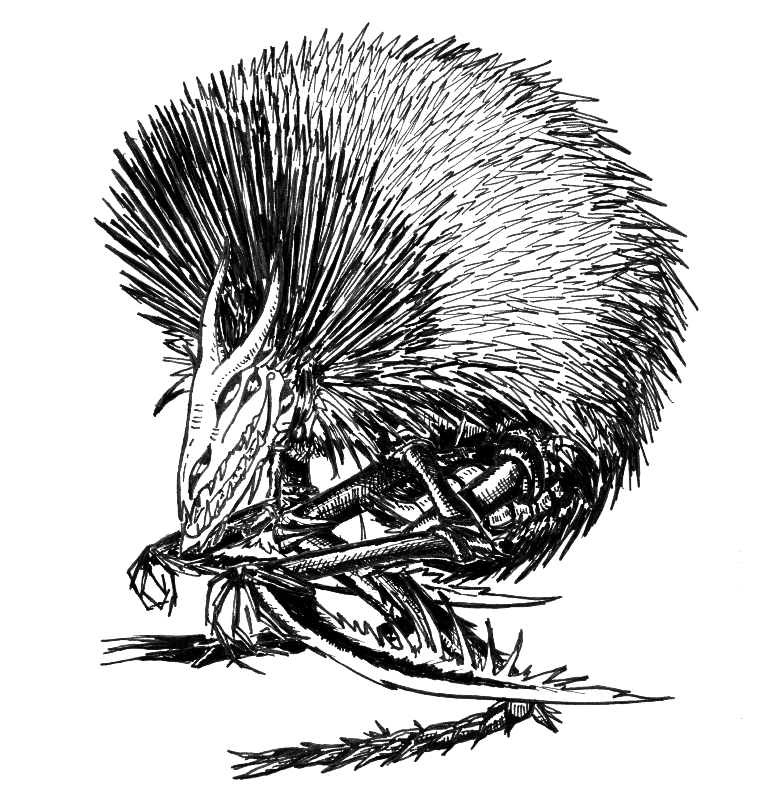
\includegraphics{benahir.eps}
\end{center}
\end{figure*}

\incubo{Benair}{23}{Terza Dimora}{Richiamabile}

Sono i pi\`u potenti tra gli incubi evocabili. Alti fino a 4 metri,
sono tozzi, scuri, curvi, hanno la schiena irta di aculei fitti,
lunghi e spessi, che possono lanciare a volont\`a. Gli arti
inferiori sono simili alle zampe di una mosca e l'addome \`e simile
a quello di un ragno. Gli arti superiori sono lunghi e
all'estremit\`a, oltre ad avere una sottilissima mano, in
corrispondenza dei polsi sono armati di affilatissime e lunghe lame
ossee, molto mobili e articolabili, con le quali possono colpire uno o
pi\`u bersagli fino a 5 m di distanza, come fossero dei lunghi
spadoni, infliggendo loro 3d8 PV/PSC di danno. La testa, allungata,
\`e provvista di bocca, in grado di mordere infliggendo 2d8 PV/PSC
di danno, e cheliceri, con un numero variabile di occhi rossi (6 o 8
sono comuni).  

Possono, a discrezione, parlare o comunicare per via
telepatica.

Sono in grado di avvolgersi a palla e di proiettarsi sui bersagli che
si trovano davanti a loro, su una linea retta, devastandoli con una
carica che infligge 5d6 PV/PSC di danno + FOR. Hanno bisogno per\`o
di 1 round per appallottolarsi.  Il loro unico punto vitale \`e
l'addome, che pu\`o essere colpito solo dal basso.

\carmostro{15+1d10}{12+1d8}{14+2d8}{14+2d8}{20+1d10}{15+1d10}{-1d10}{260}

\begin{parmostro}{Abilit\`a di Combattimento/TOT/Danno}
\item ATL/AGI/3d8
\item CAC/AGI/2d8
\item ADT/OSS+7/2d6
\end{parmostro}

\begin{parmostro}{Attacchi Particolari/TOT/Danno}
\item  Attacco a Palla/AGI/5d6
\end{parmostro}

\begin{parmostro}{Specifiche di AM/TOT}
\item Parata/AGI
\item Schivata/AGI
\end{parmostro}

\begin{parmostro}{Tecniche Speciali di AM/TOT}
\item Carica/AGI
\end{parmostro}

\begin{parmostro}{Difese}
\item Corazza di Spine (PP 10)
\end{parmostro}

\begin{parmostro}{Poteri Speciali}
\item Dolore
\item Evoca Essere Onirico II
\item Ipnosi III
\item Quadruplicazione
\item Realt\`a Virtuale
\item Scomparsa Totale
\item Scudo Psichico II
\item Sdoppiamento
\item Telecinesi
\item Tempesta di frecce
\item Viaggio Onirico
\end{parmostro}

\incubo{Morte}{$>$ 30}{Seconda Dimora}{Non Richiamabile}

L'unico essere onirico di seconda dimora di cui si abbia conoscenza
\`e l'incubo denominato Morte.

Non si conosce granch\'e di questa essenza; si sa soltanto che appare ai
vegliardi come un essere umanoide alto due metri e mezzo, vestito con
un saio scuro. Il suo viso \`e nascosto da un cappuccio dal quale si
intravedono gli occhi rossi. Regge in mano una grande falce. Non si
conoscono con esattezza i suoi poteri.


\incubo{Babau}{$>$ 30}{Prima Dimora}{Non Richiamabile}

Il Babau si manifesta raramente. \`E una creatura misteriosa, caotica,
potentissima; pu\`o apparire sotto qualsiasi aspetto e bench\'e sia
classificato come incubo non \`e ben chiaro se lo sia effettivamente
o sia un sogno.  Non esistono descrizioni pi\`u accurate.

Si sa per certo che esiste una sola entit\`a chiamata Babau, e si
suppone che questa sia la creatura pi\`u potente che abita la dimora
onirica.

\subsection{Gli Incantesimi}
\label{incillusionismo}
%----------------------------------------------------------------------------
\begin{spell}{Barriera psichica I}{Illusionismo}{Difesa}{Antimagia}
%----------------------------------------------------------------------------
\descrizione{Difende il target da tutti gli incantesimi a lui diretti nel tempo di 3 minuti, con una Base Antimagia di 10.}
%% DR DA DT DB MOD PM PF PE TL
\incvalori{15}{26}{15}{10}{1}{15}{5}{26}{2}
\parametro{Base antimagia}{10}{punti}{10}
\fineparametri
\gittatanulla
\campo{1}{target}{2}
\durata{3 min}{0}
\end{spell}
%----------------------------------------------------------------------------
\begin{spell}{Barriera psichica II}{Illusionismo}{Difesa}{Antimagia}
%----------------------------------------------------------------------------
\descrizione{Difende il target da tutti gli incantesimi nel tempo di 3 minuti, con una Base Antimagia di 20.}
%% DR DA DT DB MOD PM PF PE TL
\incvalori{25}{36}{15}{20}{1}{25}{8}{36}{4}
\parametro{Base antimagia}{20}{punti}{20}
\fineparametri
\gittatanulla
\campo{1}{target}{2}
\durata{3 min}{0}
\end{spell}
%----------------------------------------------------------------------------
\begin{spell}{Buio}{Illusionismo}{Controllo}{Illusione visiva}
%----------------------------------------------------------------------------
\descrizione{Illude i target che si trovano in un'area di 4 metri di raggio sita fino a 4 metri dal mago che la luce sia scomparsa. I target che realizzeranno un TOSS a Diff. 20 si renderanno conto che il buio \`e un'illusione e potranno rivedere la luce realizzando un TV a Diff. 20. Il buio dura 3 minuti.}
%% DR DA DT DB MOD PM PF PE TL
\incvalori{7}{27}{2}{20}{5}{7}{2}{27}{1}
\parametro{Difficolt\`a del TV e del TOSS}{20}{}{20}
\fineparametri
\gittata{4}{1}
\campo{4}{m}{4}
\durata{3 min}{0}
\end{spell}
%----------------------------------------------------------------------------
\begin{spell}{Cecit\`a}{Illusionismo}{Controllo}{Illusione visiva}
%----------------------------------------------------------------------------
\descrizione{Provoca la cecit\`a in 1 target posto ad una distanza massima di 4 metri illudendolo di essere perennemente al buio. Se il target realizza un TOSS a Diff. 25 si accorger\`a che la cecit\`a \`e un'illusione e potr\`a riprendere la vista realizzando un TV a Diff. 25.}
%% DR DA DT DB MOD PM PF PE TL
\incvalori{25}{45}{2}{25}{18}{25}{8}{45}{4}
\parametro{Difficolt\`a del TV e del TOSS}{25}{}{25}
\fineparametri
\gittata{4}{1}
\campo{1}{target}{2}
\durata{permanente }{15}
\end{spell}
%----------------------------------------------------------------------------
\begin{spell}{Concretizzazione}{Illusionismo}{Alterazione}{Creazione Esseri Viventi}
%----------------------------------------------------------------------------
\descrizione{Crea un essere vivente con massimo 30 Punti CAT richiamando dalla dimora onirica una raffigurazione di un essere vivente.}
%% DR DA DT DB MOD PM PF PE TL
\incvalori{33}{42}{29}{11}{2}{33}{11}{42}{5}
\parametro{Massa vivente}{90}{kg}{3}
\parametro{punti CAraTteristica}{30}{punti}{8}
\fineparametri
\gittata{1}{0}
\campo{1}{target}{2}
\durata{3 min}{0}
\end{spell}
%----------------------------------------------------------------------------
\begin{spell}{Concretizzazione oggetti}{Illusionismo}{Alterazione}{Creazione Oggetti}
%----------------------------------------------------------------------------
\descrizione{Crea un oggetto richiamando dalla dimora onirica una raffigurazione non vivente di un oggetto di massimo 30 kg di peso, di complessit\`a massima 8. L'oggetto sparisce dopo 3 minuti.}
%% DR DA DT DB MOD PM PF PE TL
\incvalori{21}{30}{19}{9}{2}{21}{7}{30}{3}
\parametro{Complessit\`a}{8}{}{8}
\parametro{Massa non vivente}{30}{kg}{1}
\fineparametri
\gittata{1}{0}
\campo{1}{target}{2}
\durata{3 min}{0}
\end{spell}
%----------------------------------------------------------------------------
\begin{spell}{Controllo Creatura Onirica I}{Illusionismo}{Evocazione}{Controllo}
%----------------------------------------------------------------------------
\descrizione{Consente di controllare il comportamento di una creatura onirica di potenza massima 6, situata a massimo 4 metri di distanza dal mago, per 3 minuti. Perch\'e il controllo abbia luogo, il mago deve vincere un Confronto di TV con la creatura se questa \`e una creatura errante, o realizzare un TV maggiore del TV effettuato da colui che ne ha il controllo.}
%% DR DA DT DB MOD PM PF PE TL
\incvalori{9}{23}{14}{6}{3}{9}{3}{23}{1}
\parametro{Potenza della creatura}{6}{}{6}
\fineparametri
\gittata{4}{1}
\campo{1}{target}{2}
\durata{3 min}{0}
\end{spell}
%----------------------------------------------------------------------------
\begin{spell}{Controllo Creatura Onirica II}{Illusionismo}{Evocazione}{Controllo}
%----------------------------------------------------------------------------
\descrizione{Consente di controllare il comportamento di una creatura onirica di potenza massima 15, situata a massimo 4 metri di distanza dal mago, per 3 minuti. Perch\'e il controllo abbia luogo, il mago deve vincere un Confronto di TV con la creatura se questa \`e una creatura errante o realizzare un TV maggiore del TV effettuato da colui che ne ha gi\`a il controllo.}
%% DR DA DT DB MOD PM PF PE TL
\incvalori{18}{32}{14}{15}{3}{18}{6}{32}{3}
\parametro{Potenza della creatura}{15}{}{15}
\fineparametri
\gittata{4}{1}
\campo{1}{target}{2}
\durata{3 min}{0}
\end{spell}
%----------------------------------------------------------------------------
\begin{spell}{Controllo Creatura Onirica III}{Illusionismo}{Evocazione}{Controllo}
%----------------------------------------------------------------------------
\descrizione{Consente di controllare il comportamento di una creatura onirica di potenza massima 23, situata a massimo 4 metri di distanza dal mago, per 3 minuti. Perch\'e il controllo abbia luogo, il mago deve vincere un Confronto di TV con la creatura se questa \`e una creatura errante o realizzare un TV maggiore del TV effettuato da colui che ha il controllo della creatura stessa.}
%% DR DA DT DB MOD PM PF PE TL
\incvalori{26}{40}{14}{23}{3}{26}{8}{40}{4}
\parametro{Potenza della creatura}{23}{}{23}
\fineparametri
\gittata{4}{1}
\campo{1}{target}{2}
\durata{3 min}{0}
\end{spell}
%----------------------------------------------------------------------------
\begin{spell}{Dolore}{Illusionismo}{Attacco}{Danno Netto}
%----------------------------------------------------------------------------
\descrizione{Provoca una brusca contrazione involontaria della muscolatura del target causando una dolorosa fitta che provoca 3d6 PV di danno. Il danno pu\`o essere dimezzato realizzando un TR a Diff. 16.}
%% DR DA DT DB MOD PM PF PE TL
\incvalori{25}{30}{21}{6}{3}{25}{8}{30}{4}
\parametro{Danno}{3}{d6}{6}
\fineparametri
\gittata{4}{1}
\campo{1}{target}{2}
\duratanulla
\end{spell}
%----------------------------------------------------------------------------
\begin{spell}{Evoca Essere Onirico I}{Illusionismo}{Evocazione}{Richiamo}
%----------------------------------------------------------------------------
\descrizione{Il mago richiama dalla dimora onirica un Braak, un Blink o un Greyant e gli impartisce comandi, che la creatura onirica esegue al meglio delle sue possibilit\`a, a patto che il mago vinca un confronto di TV con l'essere evocato. Perch\'e il richiamo riesca ci deve essere un adulto che dorme nel raggio di 1000 metri.}
%% DR DA DT DB MOD PM PF PE TL
\incvalori{12}{26}{18}{6}{2}{12}{4}{26}{2}
\parametro{Potenza della creatura}{6}{}{6}
\fineparametri
\gittata{1}{0}
\campo{1}{target}{2}
\durata{3 min}{0}
\end{spell}
%----------------------------------------------------------------------------
\begin{spell}{Evoca Essere Onirico II}{Illusionismo}{Evocazione}{Richiamo}
%----------------------------------------------------------------------------
\descrizione{Il mago richiama dalla dimora onirica un Bleargh, un Succube, un Tolden, un Moae o un Kartenius (o una creatura onirica di potenza inferiore) e gli impartisce comandi, che la creatura esegue al meglio delle sue possibilit\`a, a patto che il mago vinca un confronto di TV con l'essere evocato. Perch\'e il richiamo riesca ci deve essere un anziano che dorme nel raggio di 1000 metri.}
%% DR DA DT DB MOD PM PF PE TL
\incvalori{21}{35}{18}{15}{2}{21}{7}{35}{3}
\parametro{Potenza della creatura}{15}{}{15}
\fineparametri
\gittata{1}{0}
\campo{1}{target}{2}
\durata{3 min}{0}
\end{spell}
%----------------------------------------------------------------------------
\begin{spell}{Evoca Essere Onirico III}{Illusionismo}{Evocazione}{Richiamo}
%----------------------------------------------------------------------------
\descrizione{Il mago richiama dalla dimora onirica un Krull o un Benair (o una creatura onirica di potenza inferiore) e gli impartisce comandi, che la creatura esegue al meglio delle sue possibilit\`a, a patto che il mago vinca un confronto di TV con l'essere evocato. Perch\'e il richiamo riesca ci deve essere un adolescente che dorme nel raggio di 1000 metri.}
%% DR DA DT DB MOD PM PF PE TL
\incvalori{29}{43}{18}{23}{2}{29}{9}{43}{4}
\parametro{Potenza della creatura}{23}{}{23}
\fineparametri
\gittata{1}{0}
\campo{1}{target}{2}
\durata{3 min}{0}
\end{spell}
%----------------------------------------------------------------------------
\begin{spell}{Fetore}{Illusionismo}{Alterazione}{Variazione abilit\`a fisica}
%----------------------------------------------------------------------------
\descrizione{Convince i target di sentire un odore pessimo, come di uova marce ammuffite. Il risultato \`e un malus di -3 all'abilit\`a Fiutare per 3 minuti. I target possono sottrarsi agli effetti dell'incantesimo realizzando un TR a Diff. 13.}
%% DR DA DT DB MOD PM PF PE TL
\incvalori{15}{24}{18}{3}{3}{15}{5}{24}{2}
\parametro{Variazione abilit\`a}{3}{punti}{3}
\fineparametri
\gittatanulla
\campo{4}{m}{4}
\durata{3 min}{0}
\end{spell}
%----------------------------------------------------------------------------
\begin{spell}{Fitta}{Illusionismo}{Attacco}{Danno Netto}
%----------------------------------------------------------------------------
\descrizione{Provoca una brusca contrazione involontaria della muscolatura del target causando una dolorosa fitta che provoca 1d6 PV di danno. Il danno pu\`o essere dimezzato realizzando un TR a Diff. 12.}
%% DR DA DT DB MOD PM PF PE TL
\incvalori{21}{26}{21}{2}{3}{21}{7}{26}{3}
\parametro{Danno}{1}{d6}{2}
\fineparametri
\gittata{4}{1}
\campo{1}{target}{2}
\duratanulla
\end{spell}
%----------------------------------------------------------------------------
\begin{spell}{Follia}{Illusionismo}{Controllo}{Variazione PSIche}
%----------------------------------------------------------------------------
\descrizione{Toglie 10 Punti Psiche ad un target che non realizza un TV a Diff. 22. La perdita potr\`a essere curata anche con l'abilit\`a Medicina.}
%% DR DA DT DB MOD PM PF PE TL
\incvalori{20}{40}{10}{10}{20}{20}{6}{40}{3}
\parametro{Variazione caratteristica PSI}{10}{punti}{10}
\fineparametri
\gittata{4}{1}
\campo{1}{target}{2}
\durata{permanente }{15}
\bonustr{2}
\end{spell}
%----------------------------------------------------------------------------
\begin{spell}{Ilarit\`a}{Illusionismo}{Alterazione}{Variazione caratteristica fisica}
%----------------------------------------------------------------------------
\descrizione{Suscita una sensazione di ilarit\`a nei target che non realizzano un TV a Diff. 15 causando un malus di -1 alla CONC per 3 minuti a causa del gran ridere.}
%% DR DA DT DB MOD PM PF PE TL
\incvalori{15}{24}{19}{6}{-1}{15}{5}{24}{2}
\parametro{Variazione caratteristica}{1}{punto}{6}
\fineparametri
\gittatanulla
\campo{1}{m}{1}
\duratanulla
\bonustr{-1}
\end{spell}
%----------------------------------------------------------------------------
\begin{spell}{Invisibilit\`a}{Illusionismo}{Controllo}{Illusione visiva}
%----------------------------------------------------------------------------
\descrizione{Rende invisibile il mago ai target che si trovano a 10 metri o meno da lui. I target che realizzeranno un TOSS a Diff. 20 individueranno il mago e, realizzando un successivo TV a Diff. 20, potranno vederlo.}
%% DR DA DT DB MOD PM PF PE TL
\incvalori{16}{36}{2}{20}{14}{16}{5}{36}{2}
\parametro{Difficolt\`a del TV e del TOSS}{20}{}{20}
\fineparametri
\gittatanulla
\campo{10}{m}{10}
\durata{concentrazione+3 min}{5+0}
\end{spell}
%----------------------------------------------------------------------------
\begin{spell}{Ipnosi I}{Illusionismo}{Controllo}{Comando}
%----------------------------------------------------------------------------
\descrizione{Fa compiere al target che non realizza un TV a Diff. 20 un un gesto qualsiasi, anche prolungato, fino a 3 minuti. Il target deve distare 4 metri o meno dal mago.}
%% DR DA DT DB MOD PM PF PE TL
\incvalori{14}{34}{11}{20}{3}{14}{4}{34}{2}
\parametro{Difficolt\`a del TV}{20}{}{20}
\fineparametri
\gittata{4}{1}
\campo{1}{target}{2}
\durata{3 min}{0}
\end{spell}
%----------------------------------------------------------------------------
\begin{spell}{Ipnosi II}{Illusionismo}{Controllo}{Comando}
%----------------------------------------------------------------------------
\descrizione{Fa compiere ai target situati all'interno di un'area di 3 metri di raggio, che non realizzano un TV a Diff. 25 un un gesto qualsiasi, anche prolungato, fino a 3 minuti. Il centro dell'area deve distare 4 metri o meno dal mago. Il gesto \`e lo stesso per tutti i target.}
%% DR DA DT DB MOD PM PF PE TL
\incvalori{20}{40}{11}{25}{4}{20}{6}{40}{3}
\parametro{Difficolt\`a del TV}{25}{}{25}
\fineparametri
\gittata{4}{1}
\campo{3}{m}{3}
\durata{3 min}{0}
\end{spell}
%----------------------------------------------------------------------------
\begin{spell}{Ipnosi III}{Illusionismo}{Controllo}{Comando}
%----------------------------------------------------------------------------
\descrizione{Fa compiere ai target situati all'interno di un'area di 6 metri di raggio, che non realizzano un TV a Diff. 30 un un gesto qualsiasi, anche prolungato, fino a 3 minuti. Il centro dell'area deve distare 11 metri o meno dal mago. Il gesto \`e lo stesso per tutti i target.}
%% DR DA DT DB MOD PM PF PE TL
\incvalori{30}{50}{11}{30}{9}{30}{10}{50}{5}
\parametro{Difficolt\`a del TV}{30}{}{30}
\fineparametri
\gittata{11}{3}
\campo{6}{m}{6}
\durata{3 min}{0}
\end{spell}
%----------------------------------------------------------------------------
\begin{spell}{Istigazione al suicidio}{Illusionismo}{Attacco}{Morte}
%----------------------------------------------------------------------------
\descrizione{Il target che non realizza un TV a Diff. 20 si toglier\`a la vita il prima possibile. L' incantesimo agisce su un target che si trova a 1 metro o meno dal mago. Per impedire al target di suicidarsi \`e necessario effettuare  un controincantesimo a DA 35.}
%% DR DA DT DB MOD PM PF PE TL
\incvalori{30}{35}{18}{15}{2}{30}{10}{35}{5}
\parametro{Difficolt\`a del TR}{15}{}{15}
\fineparametri
\gittata{1}{0}
\campo{1}{target}{2}
\duratanulla
\end{spell}
%----------------------------------------------------------------------------
\begin{spell}{Lettura del pensiero}{Illusionismo}{Informazione}{Interrogazione}
%----------------------------------------------------------------------------
\descrizione{Legge il "pensiero superficiale" (cio\`e quello corrente) dalla mente di un target, posto fino a 4 metri di distanza dal mago. Il target pu\`o evitare l'incantesimo realizzando un TV a Diff. 20.}
%% DR DA DT DB MOD PM PF PE TL
\incvalori{13}{29}{6}{20}{3}{13}{4}{29}{2}
\parametro{Difficolt\`a del TV}{20}{}{20}
\parametro{Tempo trascorso}{0}{anni}{0}
\fineparametri
\gittata{4}{1}
\campo{1}{target}{2}
\duratanulla
\end{spell}
%----------------------------------------------------------------------------
\begin{spell}{Luci colorate}{Illusionismo}{Controllo}{Miraggio visivo}
%----------------------------------------------------------------------------
\descrizione{Manifesta un effetto luminoso colorato a scelta del mago, visibile da tutti nell'area di 4 metri. L'effetto \`e evidentemente illusorio, e chiunque lo desideri (il TV riesce automaticamente) potr\`a far scomparire l'effetto dalla sua vista.}
%% DR DA DT DB MOD PM PF PE TL
\incvalori{-14}{6}{2}{1}{3}{1}{1}{6}{1}
\parametro{Difficolt\`a del TV e del TOSS}{1}{}{1}
\fineparametri
\gittatanulla
\campo{4}{m}{4}
\durata{3 min}{0}
\end{spell}
%----------------------------------------------------------------------------
\begin{spell}{Lussuria}{Illusionismo}{Controllo}{Comando}
%----------------------------------------------------------------------------
\descrizione{Risveglia un'irresistibile frenesia nel target che non realizza un TV a Diff. 25.}
%% DR DA DT DB MOD PM PF PE TL
\incvalori{17}{37}{11}{25}{1}{17}{5}{37}{2}
\parametro{Difficolt\`a del TV}{25}{}{25}
\fineparametri
\gittatanulla
\campo{1}{target}{2}
\durata{3 min}{0}
\end{spell}
%----------------------------------------------------------------------------
\begin{spell}{Panico}{Illusionismo}{Controllo}{Variazione PSIche}
%----------------------------------------------------------------------------
\descrizione{Causa una sensazione di terrore nei target situati all'interno di un'area di 10 metri di raggio attorno all'usufruitore, tale da far impazzire per 7 minuti (-20 alla Psiche) i target che non realizzano un TV a Diff. 30.}
%% DR DA DT DB MOD PM PF PE TL
\incvalori{20}{40}{10}{20}{10}{20}{6}{40}{3}
\parametro{Variazione caratteristica PSI}{20}{punti}{20}
\fineparametri
\gittatanulla
\campo{10}{m}{10}
\durata{7 min}{1}
\end{spell}
%----------------------------------------------------------------------------
\begin{spell}{Paralisi I}{Illusionismo}{Controllo}{Comando}
%----------------------------------------------------------------------------
\descrizione{Impone ai target che non realizzano un TV a Diff. 15 di restare completamente immobili per 3 minuti. I target potranno riprendere a muoversi, se attaccati, realizzando un TV a Diff. 15.}
%% DR DA DT DB MOD PM PF PE TL
\incvalori{9}{29}{11}{15}{3}{9}{3}{29}{1}
\parametro{Difficolt\`a del TV}{15}{}{15}
\fineparametri
\gittata{4}{1}
\campo{1}{target}{2}
\durata{3 min}{0}
\end{spell}
%----------------------------------------------------------------------------
\begin{spell}{Paralisi II}{Illusionismo}{Controllo}{Comando}
%----------------------------------------------------------------------------
\descrizione{Impone a tutti gli esseri in un'area di 3 metri di raggio con centro entro 7 metri dal mago, che non realizzano un TV a Diff. 25 di restare completamente immobili per 3 minuti. I target potranno riprendere a muoversi, se attaccati, realizzando un TV a Diff. 25.}
%% DR DA DT DB MOD PM PF PE TL
\incvalori{21}{41}{11}{25}{5}{21}{7}{41}{3}
\parametro{Difficolt\`a del TV}{25}{}{25}
\fineparametri
\gittata{7}{2}
\campo{3}{m}{3}
\durata{3 min}{0}
\end{spell}
%----------------------------------------------------------------------------
\begin{spell}{Paura}{Illusionismo}{Controllo}{Variazione PSIche}
%----------------------------------------------------------------------------
\descrizione{Infonde in 1d6 di target una sensazione di paura generalizzata che comporta un malus di -10 alla Psiche per 3 minuti, se i target non realizzano un TV a Diff. 20.}
%% DR DA DT DB MOD PM PF PE TL
\incvalori{8}{28}{10}{10}{8}{8}{2}{28}{1}
\parametro{Variazione caratteristica PSI}{10}{punti}{10}
\fineparametri
\gittata{7}{2}
\campo{1}{d6 target}{6}
\durata{3 min}{0}
\end{spell}
%----------------------------------------------------------------------------
\begin{spell}{Pazzia}{Illusionismo}{Controllo}{Variazione PSIche}
%----------------------------------------------------------------------------
\descrizione{Rende pazzo un target che viene toccato dal mago, sottraendogli permanentemente 15 punti Psiche se non realizza un TV a Diff. 25.}
%% DR DA DT DB MOD PM PF PE TL
\incvalori{21}{41}{10}{15}{16}{21}{7}{41}{3}
\parametro{Variazione caratteristica PSI}{15}{punti}{15}
\fineparametri
\gittatanulla
\campo{1}{target}{2}
\durata{permanente }{15}
\end{spell}
%----------------------------------------------------------------------------
\begin{spell}{Protezione Incubi I}{Illusionismo}{Evocazione}{Protezione}
%----------------------------------------------------------------------------
\descrizione{Viene creata attorno al mago un'area di 3 metri di raggio all'interno della quale le creature oniriche di potenza inferiore o uguale a 6 non possono entrare se non realizzando un TV a Diff. 20. Realizzando un TV le creature potranno avanzare di 1 metro, subendo 1d6 PV di danno per ogni metro all'interno dell'area, L'incantesimo scompare se un essere all'interno dell'area attacca le creature dalle quali si sta proteggendo. Per ogni metro all'interno dell'area il TV delle creature \`e penalizzato di -1. L'incantesimo perdura per 3 minuti.}
%% DR DA DT DB MOD PM PF PE TL
\incvalori{8}{22}{10}{6}{6}{8}{2}{22}{1}
\parametro{Potenza della creatura}{6}{}{6}
\fineparametri
\gittatanulla
\campo{3}{m}{3}
\durata{3 min}{0}
\bonustr{4}
\end{spell}
%----------------------------------------------------------------------------
\begin{spell}{Protezione Incubi II}{Illusionismo}{Evocazione}{Protezione}
%----------------------------------------------------------------------------
\descrizione{Viene creata attorno al mago un'area di 3 metri di raggio all'interno della quale le creature oniriche di potenza inferiore o uguale a 15 non possono entrare se non realizzando un TV a Diff. 25. Realizzando un TV le creature potranno avanzare di 1 metro, subendo 1d6 PV di danno per ogni metro all'interno dell'area, L'incantesimo scompare se un essere all'interno dell'area attacca le creature dalle quali si sta proteggendo. Per ogni metro all'interno dell'area il TV delle creature \`e penalizzato di -1. L'incantesimo perdura per 3 minuti.}
%% DR DA DT DB MOD PM PF PE TL
\incvalori{13}{27}{10}{15}{2}{13}{4}{27}{2}
\parametro{Potenza della creatura}{15}{}{15}
\fineparametri
\gittatanulla
\campo{3}{m}{3}
\durata{3 min}{0}
\end{spell}
%----------------------------------------------------------------------------
\begin{spell}{Protezione Incubi III}{Illusionismo}{Evocazione}{Protezione}
%----------------------------------------------------------------------------
\descrizione{Viene creata attorno al mago un'area di 3 metri di raggio all'interno della quale le creature oniriche di potenza inferiore o pari a 23 non possono entrare se non realizzando un TV a Diff. 30. Realizzando un TV le creature potranno avanzare di 1 metro, subendo 1d6 PV di danno per ogni metro all'interno dell'area, L'incantesimo scompare se un essere all'interno dell'area attacca le creature dalle quali si sta proteggendo. Per ogni metro all'interno dell'area il TV delle creature \`e penalizzato di -1. L'incantesimo perdura per 3 minuti.}
%% DR DA DT DB MOD PM PF PE TL
\incvalori{18}{32}{10}{23}{-1}{18}{6}{32}{3}
\parametro{Potenza della creatura}{23}{}{23}
\fineparametri
\gittatanulla
\campo{3}{m}{3}
\durata{3 min}{0}
\bonustr{-3}
\end{spell}
%----------------------------------------------------------------------------
\begin{spell}{Psicosi}{Illusionismo}{Controllo}{Variazione PSIche}
%----------------------------------------------------------------------------
\descrizione{Induce in un target che non realizza un TV a Diff. 20 una psicosi che comporta la perdita permanente di 10 punti Psiche. La psicosi pu\`o essere curata con l'abilit\`a Medicina.}
%% DR DA DT DB MOD PM PF PE TL
\incvalori{17}{37}{10}{10}{17}{17}{5}{37}{2}
\parametro{Variazione caratteristica PSI}{10}{punti}{10}
\fineparametri
\gittata{1}{0}
\campo{1}{target}{2}
\durata{permanente }{15}
\end{spell}
%----------------------------------------------------------------------------
\begin{spell}{Quadruplicazione}{Illusionismo}{Controllo}{Miraggio visivo}
%----------------------------------------------------------------------------
\descrizione{Vengono create tre immagini illusorie esattamente uguali al mago, che si possono muovere all'interno di un'area di 6 metri di raggio distante fino a 10 metri dal mago stesso. Realizzando un TOSS a Diff. 25 ci si accorger\`a del miraggio, e lo si potr\`a far scomparire dalla propria vista realizzando un TV a 25. Il miraggio permane per 7 minuti.}
%% DR DA DT DB MOD PM PF PE TL
\incvalori{17}{37}{2}{25}{10}{17}{5}{37}{2}
\parametro{Difficolt\`a del TV e del TOSS}{25}{}{25}
\fineparametri
\gittata{10}{3}
\campo{6}{m}{6}
\durata{7 min}{1}
\end{spell}
%----------------------------------------------------------------------------
\begin{spell}{Realt\`a virtuale}{Illusionismo}{Attacco}{Morte}
%----------------------------------------------------------------------------
\descrizione{Proietta la mente del target in un mondo onirico virtuale a scelta del mago, causandone di fatto la morte (coma irreversibile) se questi non realizza un TV a Diff. 20. L'incantesimo \`e permanente ma reversibile (dal mondo onirico virtuale si pu\`o ritornare effettuando lo stesso incantesimo sul corpo). L'uccisione del corpo inerte provoca la morte definitiva del target, dalla quale si pu\`o resuscitare normalmente.}
%% DR DA DT DB MOD PM PF PE TL
\incvalori{35}{40}{18}{20}{2}{35}{11}{40}{5}
\parametro{Difficolt\`a del TR}{20}{}{20}
\fineparametri
\gittata{1}{0}
\campo{1}{target}{2}
\duratanulla
\end{spell}
%----------------------------------------------------------------------------
\begin{spell}{Scomparsa totale}{Illusionismo}{Controllo}{Illusione completa}
%----------------------------------------------------------------------------
\descrizione{Il target non viene visto, udito n\'e percepito con nessuno dei sensi da nessun essere che sta ad una distanza inferiore a 10 metri. La presenza del mago pu\`o essere percepita con un TOSS a Diff. 30. Un successivo TV a Diff. 30 render\`a visibile il mago agli occhi di chi lo realizza. L'incantesimo pu\`o essere lanciato sul mago stesso o su un target a contatto.}
%% DR DA DT DB MOD PM PF PE TL
\incvalori{28}{48}{9}{30}{9}{28}{9}{48}{4}
\parametro{Difficolt\`a del TV e del TOSS}{30}{}{30}
\fineparametri
\gittatanulla
\campo{10}{m}{10}
\durata{3 min}{0}
\end{spell}
%----------------------------------------------------------------------------
\begin{spell}{Scudo Psichico}{Illusionismo}{Difesa}{Scudo antidinamico}
%----------------------------------------------------------------------------
\descrizione{Genera attorno al target uno scudo di energia psichica attivo per 3 minuti che divide per 5 tutti i danni da punta, taglio e botta e da Attacco/Danno mirato.}
%% DR DA DT DB MOD PM PF PE TL
\incvalori{36}{47}{21}{25}{1}{36}{12}{47}{6}
\parametro{Divisore}{5}{unit\`a}{25}
\fineparametri
\gittatanulla
\campo{1}{target}{2}
\durata{3 min}{0}
\end{spell}
%----------------------------------------------------------------------------
\begin{spell}{Sdoppiamento}{Illusionismo}{Controllo}{Illusione completa}
%----------------------------------------------------------------------------
\descrizione{Qualunque essere, situato a meno di 10 metri dal mago, vedr\`a una immagine illusoria di costui, perfettamente identica anche al tatto, all'olfatto e all'udito. Se un target realizza un TOSS a Diff. 30, a cui far\`a seguito un TV di pari Diff., l'illusione sar\`a, per lui, dissolta. L'immagine permane per 3 minuti.}
%% DR DA DT DB MOD PM PF PE TL
\incvalori{28}{48}{9}{30}{9}{28}{9}{48}{4}
\parametro{Difficolt\`a del TV e del TOSS}{30}{}{30}
\fineparametri
\gittatanulla
\campo{10}{m}{10}
\durata{3 min}{0}
\end{spell}
%----------------------------------------------------------------------------
\begin{spell}{Sfera sonica}{Illusionismo}{Attacco}{Danno Netto}
%----------------------------------------------------------------------------
\descrizione{Trasmette telepaticamente un suono acutissimo che causa convulsioni ai target situati all'interno di un'area di 3 metri di raggio con centro situato a 4 metri o meno dal mago. Le convulsioni causano 3d6 PV di danno, dimezzabili con un TV a Diff. 16.}
%% DR DA DT DB MOD PM PF PE TL
\incvalori{26}{31}{21}{6}{4}{26}{8}{31}{4}
\parametro{Danno}{3}{d6}{6}
\fineparametri
\gittata{4}{1}
\campo{3}{m}{3}
\duratanulla
\end{spell}
%----------------------------------------------------------------------------
\begin{spell}{Sonno I}{Illusionismo}{Controllo}{Comando}
%----------------------------------------------------------------------------
\descrizione{Addormenta un target fino a 4 metri di distanza per 3 minuti. Al termine dei 3 minuti il target continuer\`a a dormire per 1d8 ore se non viene svegliato. Il target pu\`o sottrarsi all'incantesimo realizzando un TV a Diff. 15.}
%% DR DA DT DB MOD PM PF PE TL
\incvalori{9}{29}{11}{15}{3}{9}{3}{29}{1}
\parametro{Difficolt\`a del TV}{15}{}{15}
\fineparametri
\gittata{4}{1}
\campo{1}{target}{2}
\durata{3 min}{0}
\end{spell}
%----------------------------------------------------------------------------
\begin{spell}{Sonno II}{Illusionismo}{Controllo}{Comando}
%----------------------------------------------------------------------------
\descrizione{Addormenta un target fino a 10 metri di distanza per 3 minuti. Al termine dei 3 minuti il target continuer\`a a dormire per 1d8 ore se non viene svegliato. Il target pu\`o sottrarsi all'incantesimo realizzando un TV a Diff. 20.}
%% DR DA DT DB MOD PM PF PE TL
\incvalori{16}{36}{11}{20}{5}{16}{5}{36}{2}
\parametro{Difficolt\`a del TV}{20}{}{20}
\fineparametri
\gittata{10}{3}
\campo{1}{target}{2}
\durata{3 min}{0}
\end{spell}
%----------------------------------------------------------------------------
\begin{spell}{Sonno profondo}{Illusionismo}{Controllo}{Comando}
%----------------------------------------------------------------------------
\descrizione{Addormenta permanentemente un target fino a 4 metri di distanza se questi non realizza un TV a Diff. 20. L'incantesimo pu\`o essere sciolto automaticamente dopo un certo evento o dopo un tempo a scelta del mago (es. dopo 100 anni o al bacio di un principe azzurro...).}
%% DR DA DT DB MOD PM PF PE TL
\incvalori{29}{49}{11}{20}{18}{29}{9}{49}{4}
\parametro{Difficolt\`a del TV}{20}{}{20}
\fineparametri
\gittata{4}{1}
\campo{1}{target}{2}
\durata{permanente }{15}
\end{spell}
%----------------------------------------------------------------------------
\begin{spell}{Stordimento}{Illusionismo}{Attacco}{Stordimento}
%----------------------------------------------------------------------------
\descrizione{Causa l'inabilitazione di un target per stordimento per il round in corso e per quello successivo. Il target deve trovarsi a 4 metri o meno dal mago. L'incantesimo non ha effetto se il target realizza un TR a Diff. 15.}
%% DR DA DT DB MOD PM PF PE TL
\incvalori{22}{27}{9}{15}{3}{22}{7}{27}{3}
\parametro{Difficolt\`a del TR}{15}{}{15}
\fineparametri
\gittata{4}{1}
\campo{1}{target}{2}
\duratanulla
\end{spell}
%----------------------------------------------------------------------------
\begin{spell}{Telecinesi}{Illusionismo}{Alterazione}{Spostamento 3 dimensioni}
%----------------------------------------------------------------------------
\descrizione{Consente di spostare per 3 minuti fino a 2 oggetti (ciascuno di 100 kg di massa non vivente e 90 kg di massa vivente) che si trovano inizialmente ad una distanza massima di 4 metri dal mago, ad una velocit\`a massima di 60 km/h. Esseri viventi si possono opporre all'incantesimo realizzando un TV a Diff. 20.}
%% DR DA DT DB MOD PM PF PE TL
\incvalori{25}{34}{19}{10}{5}{25}{8}{34}{4}
\parametro{Massa vivente}{90}{kg}{3}
\parametro{Velocit\`a}{60}{km/h}{6}
\parametro{Massa non vivente}{100}{kg}{1}
\fineparametri
\gittata{4}{1}
\campo{2}{target}{4}
\durata{3 min}{0}
\end{spell}
%----------------------------------------------------------------------------
\begin{spell}{Telepatia}{Illusionismo}{Informazione}{Trasmissione+Ricezione}
%----------------------------------------------------------------------------
\descrizione{Consente al target una comunicazione telepatica nei due sensi, sotto forma di parole con un essere che si trova a meno di 100 metri dal target.  \`E necessario che il target e l'essere con cui comunica parlino la stessa lingua, per capirsi. Il target \`e colui che inizia la comunicazione, e deve trovarsi a contatto con il mago.}
%% DR DA DT DB MOD PM PF PE TL
\incvalori{14}{30}{15}{14}{1}{14}{4}{30}{2}
\parametro{Complessit\`a}{6}{}{6}
\parametro{Distanza}{100}{m}{8}
\fineparametri
\gittatanulla
\campo{1}{target}{2}
\durata{3 min}{0}
\end{spell}
%----------------------------------------------------------------------------
\begin{spell}{Tempesta di frecce}{Illusionismo}{Attacco}{Danno Netto}
%----------------------------------------------------------------------------
\descrizione{Fa credere agli esseri all'interno di un'area di 1 metro di raggio di essere vittima di una tempesta di frecce acuminate, causando 6d6 PV di danno. I danni si manifesteranno realmente. Realizzando un TR a Diff. 22 il danno potr\`a essere dimezzato.}
%% DR DA DT DB MOD PM PF PE TL
\incvalori{30}{35}{21}{12}{2}{30}{10}{35}{5}
\parametro{Danno}{6}{d6}{12}
\fineparametri
\gittata{4}{1}
\campo{1}{m}{1}
\duratanulla
\end{spell}
%----------------------------------------------------------------------------
\begin{spell}{Velo d'ombra}{Illusionismo}{Controllo}{Illusione visiva}
%----------------------------------------------------------------------------
\descrizione{Rende il mago totalmente simile ad un'ombra, rendendogli possibile nascondersi totalmente al buio, agli occhi di coloro che si trovano a meno di 14 metri da lui. L'incantesimo perdura per tutto il tempo durante il quale il mago focalizza la sua concentrazione sull'incantesimo. Al momento della perdita di concentrazione l'effetto di invisibilt\`a prosegue per 3 minuti. Un TOSS a Diff. 25 far\`a intuire ai target la presenza del mago e un successivo TV alla stessa Diff. render\`a visibile il mago agli occhi di chi lo realizza. Il TOSS potr\`a essere ripetuto ogni volta che il mago viene individuato attraverso rumori, odori o sensazioni tattili.}
%% DR DA DT DB MOD PM PF PE TL
\incvalori{25}{45}{2}{25}{18}{25}{8}{45}{4}
\parametro{Difficolt\`a del TV e del TOSS}{25}{}{25}
\fineparametri
\gittatanulla
\campo{14}{m}{14}
\durata{concentrazione+3 min}{5+0}
\end{spell}
%----------------------------------------------------------------------------
\begin{spell}{Viaggio onirico}{Illusionismo}{Alterazione}{Teletrasporto standard}
%----------------------------------------------------------------------------
\descrizione{Teletrasporta istantaneamente attraverso la Dimora Onirica il target (90 kg + 100 kg di equipaggiamento) ad una distanza massima di 10 km in un punto in cui il target abbia dormito per almeno 1 ora Il target potrebbe subire danni all'arrivo a discrezione del Master.}
%% DR DA DT DB MOD PM PF PE TL
\incvalori{35}{44}{19}{24}{1}{35}{11}{44}{5}
\parametro{Massa vivente}{90}{kg}{3}
\parametro{Massa non vivente}{100}{kg}{1}
\parametro{Distanza di spostamento}{10000}{m}{20}
\fineparametri
\gittatanulla
\campo{1}{target}{2}
\duratanulla
\end{spell}
%----------------------------------------------------------------------------
\begin{spell}{Volont\`a}{Illusionismo}{Controllo}{Variazione VOLont\`a}
%----------------------------------------------------------------------------
\descrizione{Attribuisce ad un target un bonus di +2 alla VOLont\`a per 3 minuti, purch\'e questi sia a contatto col mago.}
%% DR DA DT DB MOD PM PF PE TL
\incvalori{12}{32}{19}{12}{1}{12}{4}{32}{2}
\parametro{Variazione caratteristica}{2}{punti}{12}
\fineparametri
\gittatanulla
\campo{1}{target}{2}
\durata{3 min}{0}
\end{spell}


\vspace{12cm}\vfill\vfill\filler{libro1.eps}

%%---------------------------------------------------------------------------
\vfill\section{Necromanzia} 
%%---------------------------------------------------------------------------

\Simbolo{simb_nec.eps}


Primo piatto della bilancia nel regno della
magia Vimohr. La Necromanzia o magia delle tenebre come viene detta in Novese,
o magia dell'Oblio eterno in Elfico, presiede il potere sulla morte e sull'usura
del tempo.

\subsection{Dominio}

I poteri e gli incantesimi dei necromanti sono sempre strettamente
legati alla morte, alla malattia, alla decadenza. La Scuola \`e in
contatto magico con il Limbo, una sorta di dimensione crepuscolare al
confine tra il Mondo Reale (o Piano Materiale) e il mondo dei morti.

Il Limbo \`e la dimora degli spiriti dei morti che non trovano
riposo, delle anime erranti e dei non-morti. Le creature incorporee
del Limbo possono essere evocate solamente dai necromanti.

Il simbolo dei necromanti \`e una luna nascente stilizzata.

\subsection{Limiti e Peculiarit\`a}  

Gli incantesimi di ``cura'' (Difesa/Cura) devono attingere la ``vita''
(PV, PM, PF, PSC, PSI) da esseri viventi. Se l'essere da cui si tenta
di prelevare la ``vita'' realizza un TR, l'incantesimo non ha effetto.
Questi incantesimi funzionano solo con gittata ``a contatto''.

\es{Alice Ryan, necromante Umbra, ha subito 4 PSC (e 4 PV) di danno al
  braccio destro, e necessita di cure. Decide di lanciare un
  incantesimo di ``cura ferite'', per recuperare 1d6 PV e PSC. Per
  fare ci\`o \`e costretto a trovare una fonte da cui attingere.
  Alice riesce a catturare viva una lepre che si aggirava nei paraggi
  e decide di usarla come ``fonte''. Alice lancia l'incantesimo, la
  lepre effettua il TR e lo fallisce. Alice pu\`o recuperare 1d6 PSC
  e PV prelevandoli dalla lepre, che perde i PV corrispondenti. Se la
  lepre avesse realizzato il TR l'incantesimo non avrebbe avuto
  successo}

Questa scuola ha anche un limitato potere sulla vita, poich\'e \`e
in grado di dare riposo alle essenze non morte mandandole dal Limbo
alla loro destinazione finale. \`E l'unica scuola che pu\`o evocare,
controllare, creare ed animare le creature non-morte.

\subsection{Potenzialit\`a}  

\begin{tabular}{lc}
  Evocazione& 13 \\
  Alterazione& 12 \\
  Controllo& 11\\
  Informazione& 17 \\
  Difesa& 5 \\
  Attacco& 17\\
\end{tabular}

\subsection{Leggi dell'uso} 
\begin{enumerate}\itemsep -6pt
\item Non contattare il Re Ombra. 
\item Non lasciare liberi gli esseri del limbo.
\item Non lasciare liberi i Non-Morti creati. 
\end{enumerate}


\subsection{Gli Esseri del Limbo}

 Le creature
del limbo possono essere distinte in tre generi, a seconda dello stato della
loro essenza vitale o della causa del decesso. 

I tre generi non indicano necessariamente
un maggiore o minore potere o una diversa gerarchia all'interno delle cinque
``cerchie''. 
\begin{description}
\item{\bf Gli spiriti irrequieti} sono le essenze vitali di coloro che sono
morti in modo violento e improvviso e rimangono in genere legati al luogo teatro
del loro decesso. A volte pu\`o accadere comunque che un non morto di maggior
potenza proponga di liberarli dalla loro prigionia in cambio del loro perenne
asservimento. Gli spiriti irrequieti hanno natura incorporea e non possono essere
danneggiati in tale forma. 

\item{\bf Le anime erranti} sono le essenze vitali delle creature
che il Re Ombra ha deciso di prendere per s\`e inviando al momento della morte
un Boia a ghermirne l'anima. Esse non hanno una dimora fissa ma vagano nel limbo
o nel Piano Materiale senza una meta precisa fino a che non riescono ad affrancarsi
dal loro stato. Anche le anime erranti hanno natura incorporea e non possono
essere danneggiate in tale forma. 

\item{\bf I Non Morti} sono i corpi (o i loro resti) dei morti che
  acquistano una nuova esistenza, in seguito al procedimento di
  creazione operato da un necromante o per intervento di un essere del
  Limbo di seconda o prima cerchia. La creazione magica di un Non
  Morto \`e caratterizzata dall'assenza dell'anima e dalla mancanza
  di memoria della vita precedente. I Non Morti sono corporei.  Per
  creare un non morto si usa un incantesimo di Evocazione/Richiamo
  ``applicandolo'' ad un cadavere.

\end{description}

Le creature del limbo possono essere richiamate se sono di natura
incorporea, mentre devono essere create a partire da resti o cadaveri
di creature in precedenza viventi se di natura corporea.

Tutte le creature del limbo sono
immuni a veleni, droghe e malattie e agli incantesimi di morte che
colpiscono gli esseri viventi. 

L'unico modo per far cessare la loro esistenza \`e la
\textbf{dismissione} dell'essenza vitale, con un incantesimo di
morte che abbia come destinatarie solo le creature del limbo. La
dismissione \`e prerogativa dei necromanti. La dismissione si
pu\`o ottenere anche distruggendo completamenete il corpo di un
Non Morto o decapitandolo. Riducendo a zero i PV di una creatura
incorporea la sua essenza viene dispersa temporaneamente per 1d6
anni, ricomponendosi poi senza memoria degli eventi passati.

Nel Limbo le creature sono disposte in ordine gerarchico in cinque
Cerchie. Ogni cerchia ha il comando sulle cerchie precedenti.

\nonmorto{Zombo (pl. Zombi)}{1}{Quinta Cerchia}{Creabile}

Lo zombo viene animato tramite un procedimento di creazione
utilizzando un cadavere (di qualunque tipo) o assemblando resti di
pi\`u cadaveri.

Pu\`o presentarsi anche incompleto, privo di uno o pi\`u arti (con
gli evidenti malus che ci\`o comporta), o con alcune parti del corpo
decomposte, se ad esempio sar\`a sprovvisto di corde vocali non
potr\`a parlare e via dicendo. 

Normalmente emana il tipico odore di carne in decomposizione, ci\`o
comporta che chiunque disti da lui meno di 3 metri debba realizzare un
TR a difficolt\`a 20 o restare stordito per il round in corso. Il TR
va ripetuto dopo ogni round sinch\'e non viene realizzato.

Lo zombo pu\`o utilizzare armi e indossare armature e le abilit\`a
di combattimento hanno un TOT pari all'AGI.

Lo zombo inoltre pu\`o mordere infliggendo 1d6 PV/PSC di danno.

Per la creazione di uno zombo \`e necessario
possedere un cadavere completo (o quasi) o assemblato. La sua
creazione richiede il lancio di un incantesimo di Richiamo.

\carmostro{6+1d6}{4+2d8}{8+1d8}{6+1d6}{12+1d8}{1d20}{1d20-4}{20}

\begin{parmostro}{Abilit\`a di Combattimento/TOT/Danno}
\item CAC/AGI/Danno normale
\item  ATL o ABL, ecc./AGI/Danno normale
\end{parmostro}

\begin{parmostro}{Attacchi Particolari/TOT/Danno}
\item  Morso/AGI/1d6
\end{parmostro}

\begin{parmostro}{Difese}
\item Armature a PP variabile
\end{parmostro}

\nonmorto{Scheletro}{1}{Quinta Cerchia}{Creabile} 

\`E un Non Morto creato utilizzando le ossa di un cadavere, non ha di
norma la capacit\`a di parlare ma il suo creatore pu\`o disporre
diversamente.  Quando lo si vede per la prima volta \`e necessario
realizzare un TP a difficolt\`a 20 o restare terrorizzati per un
round. 

La sua creazione richiede il tempo necessario a disossare il cadavere
e riassemblare lo scheletro oltre al lancio di un incantesimo di
Richiamo.

Se lo scheletro \`e gi\`a spolpato (ed \`e completo)
la sua creazione richiede soltanto il lancio di un incantesimo di
Richiamo. 

Lo Scheletro pu\`o indossare armature e brandire armi,

Il TOT nelle Abilit\`a di Combattimento \`e pari al valore della sua
AGI.


\carmostro{10+1d6}{4+2d8}{6+1d6}{10+1d6} {12+1d8}{1d20}{3-1d6}{30}

\begin{parmostro}{Abilit\`a di Combattimento/TOT/Danno}
\item CAC/AGI/Danno normale
\item ATL o ABL, ecc./AGI/Danno normale
\end{parmostro}

\begin{parmostro}{Difese}
\item Armature a PP variabile
\end{parmostro}


\spirito{Poltergeist}{4}{Quinta Cerchia}{Richiamabile}

\`El'essenza vitale di un bambino che si manifesta in maniera
burlona. Talvolta, gli scherzi combinati da questi mattacchioni
possono essere anche molto dannosi.

I Poltergeist sono incorporei ed invisibili, ma perdono tale
invisibilit\`a quando decidono di attaccare con il loro Tocco
Mortale, mentre possono essere colpiti da armi non magiche anche se
incorporei. Per attaccare, di norma, scagliano oggetti contro la
vittima con la telecinesi (che si utilizza come una normale
abilit\`a di combattimento o standard) che permette loro di spostare
oggetti pesanti fino a 100 kg ad una velocit\`a di 100 km/h. 
Il danno inferto dipender\`a dall'oggetto scagliato. 

Le loro abilit\`a di combattimento hanno un TOT pari al valore della
loro AGI.

Si spostano fluttuando ad una velocit\`a massima di 20 metri per
round.

Non possono parlare ma comunicano con la telepatia. \`E possibile
individuarli poich\'e non di rado emettono delle agghiaccianti risatine.

La prima volta che si sente il loro sinistro verso
occorrer\`a realizzare un TP a difficolt\`a 20 o restare storditi
per il round in corso.

\carmostro{1d20}{4+2d8}{6+1d6}
{12+1d10}{12+1d8}{19+1d6}{-}{105}

\begin{parmostro}{Abilit\`a di Combattimento/TOT/Danno}
\item AO(con Telecinesi)/AGI/Variabile
\item CAC/AGI/Danno normale
\end{parmostro}

\begin{parmostro}{Difese}
\item Invisibilit\`a
\end{parmostro}

\begin{parmostro}{Poteri Speciali}
\item Terrore I
\item Tocco Mortale II
\end{parmostro}

\anima{Spettro}{6}{Quinta Cerchia}{Richiamabile}

Sono le essenze vitali di animali sia esistenti che estinti. Hanno la
forma del rispettivo animale ma di un uniforme colore grigio nebbia;
della nebbia hanno anche la consistenza; quando stanno portando un
attacco diventano corporei e solo in questo momento possono essere
danneggiati da armi non magiche.

Il loro comportamento rispecchia quello dell'animale che erano, salvo
non abbiano ordini contrari in tal senso o non vengano attaccati, nel
qual caso diventano ostili. 

Possono essere evocati ma non creati; la specie dell'animale viene
stabilita dal Master dopo il lancio dei dadi per l'attribuzione delle
caratteristiche.

Quando acquistano consistenza possono portare gli attacchi fisici
propri dell'animale, infliggendo lo stesso danno. Le loro abilit\`a
di combattimento hanno un TOT pari al valore della loro AGI.

Sono in grado di emanare un'aura di terrore, che comporta per chi
si trova a meno di 3 metri da loro, la realizzazione di un TV a
difficolt\`a 15 per evitare di restare storditi per il round in
corso e quello seguente.

Se toccano le vittime quando sono incorporei possono
infliggere l'incantesimo Tocco Mortale I. 

\carmostro{2d6}{4+2d8}{3d10}{3d10}{3d10}{3d10}{3-1d4}{75}

\begin{parmostro}{Abilit\`a di Combattimento/TOT/Danno}
\item CAC/AGI/Danno normale
\end{parmostro}

\begin{parmostro}{Difese}
\item Incorporeit\`a
\end{parmostro}

\begin{parmostro}{Poteri Speciali}
\item Terrore I
\item Tocco mortale I
\end{parmostro}


\nonmorto{Mummia}{8}{Quarta Cerchia}{Creabile} 

\`E un Non Morto creato tramite il procedimento di mummificazione,
avente per base un cadavere di umanoide ``fresco'', cio\'e morto da
non pi\`u di 10 giorni.

Il processo di mummificazione richiede 6 ore. Solo dopo aver
mummificato il cadavere \`e necessario lanciare l'incantesimo di
Richiamo.

La Mummia si presenta di solito come un cadavere ricoperto da bende,
ma non \`e impossibile che si presenti come un ``Ghoul'', un essere
umanoide con occhi sporgenti, ventre pronunciato, braccia e mani
diafane ed allungate e dal colorito grigio-terra. 

La Mummia pu\`o brandire armi e le sue abilit\`a di combattimento
hanno un TOT pari al valore della sua AGI. La mummia inoltre pu\`o
scagliare le sue bende fino a 3 metri di distanza per bloccare la
vittima.  

Le bende della mummia e la pelle del Ghoul offrono una
protezione pari a 3 PP.  

Sono in grado, qualora il loro attacco abbia successo, di infliggere
Malattia I e Tocco Mortale. Le mummie possono terrorizzare le vittime.

\carmostro{10+1d10}{4+2d8}{12+1d10}{12+1d10}{
12+1d10}{4+2d8}{3-1d6}{150}

\begin{parmostro}{Abilit\`a di Combattimento/TOT/Danno}
\item CAC/AGI/Danno normale
\item ABC o AIA, ecc.  /AGI/Danno normale
\end{parmostro}

\begin{parmostro}{Specifiche di AM/TOT/BON}
\item Presa (Bende)/AGI/BON Presa
\end{parmostro}

\begin{parmostro}{Difese}
\item Bende o Pelle coriacea (PP 3)
\end{parmostro}

\begin{parmostro}{Poteri Speciali}
\item Malattia I
\item Terrore II
\item Tocco Mortale II
\end{parmostro}

\spirito{Anima}{10}{Quarta Cerchia}{Richiamabile}

\`E uno spirito irrequieto, la sua essenza vitale proviene da un
essere deceduto di morte violenta. Essa si presenta come un corpo
traslucido, semitrasparente, di colore verde-azzurro e con un volto
dall'espressione contrita.

Solitamente recher\`a in mano un oggetto a ricordo della sua vita
passata oppure l'arma che ha cagionato il decesso. Finch\'e la sua
morte non viene vendicata, la sua esistenza rimane vincolata al luogo
in cui \`e avvenuto il decesso.

L'anima \`e fondamentalmente un'essenza triste e solitaria, legata al
suo sfortunato destino; difficilmente sar\`a ostile, a meno che non
venga attaccata o non abbia avuto specifici ordini al riguardo. In tal
caso potrebbe assumere un aspetto deforme e maligno.

Essa \`e danneggiabile dalle sole armi magiche quando conserva
l'incorporeit\`a; nel momento in cui sferra attacchi fisici diviene
corporea e danneggiabile da armi non magiche.

Le sue abilit\`a di combattimento hanno un TOT pari al valore della
sua AGI.

 L'Anima \`e legata alla memoria delle persone che la
conoscevano in vita. Quando nessuno pi\`u conserver\`a memoria di
colui che \`e divenuto Anima, questa si trasformer\`a in uno
Spirito. 

Essa pu\`o attaccare con il suo Tocco Mortale. \`E in grado
di terrorizzare le sue vittime e di cagionarne la morte. \`E in grado
di utilizzare il potere di Protezione Non Morti I.

\carmostro{
4+2d8}{8+2d6}{10+2d6}{10+2d6}{10+2d6}{19+1d6}{
1d20-3}{135}

\begin{parmostro}{Abilit\`a di Combattimento/TOT/Danno}
\item CAC/AGI/Danno normale
\item ATL, ABC, ecc./AGI/Danno normale
\end{parmostro}

\begin{parmostro}{Difese}
\item  Incorporeit\`a
\end{parmostro}

\begin{parmostro}{Poteri Speciali}
\item Morte I
\item Protezione Non Morti I
\item Terrore II
\item Tocco Mortale II
\end{parmostro}

\spirito{Spirito}{11}{Quarta Cerchia}{Richiamabile}

La sua essenza vitale proviene di regola dai condannati a morte. Gli
spiriti sono maligni e hanno una spiccata propensione a provocare
dolore e sofferenza ai mortali. 

Gli spiriti appaiono come informi chiazze d'ombra semitrasparente ed
in questo stato non possono essere danneggiati da armi non magiche.
Per portare attacchi fisici devono diventare corporei.

Ogni attacco fisico \`e in grado di inoculare veleno (Peebera) oltre
ad infliggere normale danno. Quando diventano corporei sono soliti
brandire armi.

Le loro abilit\`a di
combattimento hanno un TOT pari al valore della loro AGI. Hanno il
potere di terrorizzare le vittime. 

Possono infliggere il Tocco Mortale
e sono in grado di dismettere gli esseri di Quinta cerchia.  Sono in grado
di utilizzare il potere di Protezione Non Morti I. 

\carmostro{4+2d8}{8+2d6}{10+2d6}{10+2d6}{10+2d6}{19+1d6}{-}{ 150}

\begin{parmostro}{Abilit\`a di Combattimento/TOT/Danno}
\item ATL o ADT, ecc./AGI/Danno normale + veleno
\item CAC/AGI/Danno normale + veleno
\end{parmostro}

\begin{parmostro}{Difese}
\item Incorporeit\`a
\end{parmostro}

\begin{parmostro}{Poteri Speciali}
\item Dismissione I
\item Morte I
\item Protezione Non Morti I
\item Terrore II
\item Tocco Mortale II
\end{parmostro}

\anima{Viaggiatori}{14}{Quarta Cerchia}{Richiamabile}

Essi sono la magica prole del Re Ombra la cui essenza vitale \`e
stata strappata ai bambini non nati. Essi incarnano il puro e semplice
odio per la vita. Hanno le sembianze di feti umanoidi avvolti da una
sacca semitrasparente piena di liquido amniotico.

Fluttuano incessantemente nell'aria ad una velocit\`a massima di 20
metri per round, come i poltergeist usano la telecinesi per spostare
oggetti, ma sono in grado di muovere a 100 km/h oggetti pesanti fino a
300 kg, e comunicano attraverso la telepatia.

Le loro abilit\`a di combattimento hanno un TOT pari al valore della
loro AGI. La sacca offre una protezione pari a 5 PP. Sono in grado di
utilizzare i poteri di Dito III, Schifo II, Malattia II,
Decomposizione, Catalessi, Dismissione V e IV cerchia, protezione Non
Morti I. Alla loro vista occorre realizzare un TP a difficolt\`a 20,
per evitare di restare storditi per il round in corso. 

Il Tiro va
ripetuto ogni round fino a che non viene realizzato.

\carmostro{10+2d6}{8+2d6}{10+2d6}{15+1d10}{15+1d10}{19+1d6}
{-1d6}{165}

\begin{parmostro}{Abilit\`a di Combattimento/TOT/Danno}
\item AO (con Telecinesi)/AGI/Variabile
\item CAC/AGI/Danno normale
\end{parmostro}

\begin{parmostro}{Difese}
\item Sacca (PP 5)
\end{parmostro}

\begin{parmostro}{Poteri Speciali}
\item Catalessi
\item Decomposizione
\item Dismissione I
\item Dismissione II
\item Dito III
\item Malattia II
\item Protezione Non Morti I
\item Schifo II
\end{parmostro}

\anima{Banshee}{16}{Terza Cerchia}{Richiamabile}

La loro essenza vitale proviene da femmine di una qualsiasi razza ed
etnia umanoide. La leggenda vuole che la loro anima sia vincolata al
Limbo perch\'e maledetta prima del decesso.

\pinup{banshee.eps}{Banshee}

Sono bellissime, molto pallide e portano lunghi capelli bianchi.
Secondo le leggende pi\`u diffuse, il loro compito principale \`e
quello di annunciare la morte ai vivi, mostrandosi in prossimit\`a
delle loro abitazioni e cantando una nenia per loro.

Per mostrarsi devono diventare corporee, altrimenti sono eteree ed
invisibili. Solo in forma corporea possono portare i loro attacchi
fisici ed utilizzare i loro poteri.

Le loro abilit\`a di combattimento hanno un TOT pari al valore della
loro AGI. La loro pelle \`e molto elastica e offre una protezione
pari a 3 PP. Il loro potere pi\`u terribile \`e il lamento
straziante, combinazione dei poteri Urlo e Visione di Morte, che porta
alla morte o alla pazzia chi lo ode.

Possono utilizzare i poteri di Tocco Mortale e Invecchiamento,
terrorizzare le loro vittime, congelarle, e contagiare loro malattie.

Quando vengono richiamate assumono immediatamente forma corporea.

\carmostro{10+2d6}{12+1d8}{15+1d10}{10+2d6}{15+1d10}{15+1d10}{15+1d10}{180}

\begin{parmostro}{Abilit\`a di comb/TOT/Danno}
\item CAC/AGI/Danno normale
\end{parmostro}

\begin{parmostro}{Difese}
\item Pelle elastica (PP 3)
\end{parmostro}

\begin{parmostro}{Poteri speciali}
\item Dismissione I
\item Dismissione II
\item Gelo I
\item Invecchiamento
\item Lamento (Urlo + Visione di Morte)
\item Malattia II
\item Protezione Non Morti I
\item Protezione Non Morti II Terrore II
\item Tocco Mortale II
\end{parmostro}

\nonmorto{Angelo nero}{19}{Terza Cerchia}{Creabile}

L'angelo nero \`e un non morto frutto di una creazione operata sul
cadavere di un adolescente di qualunque razza ed etnia. Dopo il
procedimento di creazione che richiede anche il lancio di un
incantesimo di Richiamo, il cadavere diventa nero, salvo che per gli
occhi gialli, e dalla sua schiena fuoriescono delle grosse ali di
corvo atte al volo. 

Gli arti superiori si allungano e le mani divengono artigli. 

Secondo le leggende gli Angeli Neri sono acerrimi nemici degli
angeli Adonai.

Il TOT delle abilit\`a di
combattimento \`e pari all'AGI. Gli artigli delle mani sono in grado
di infliggere 2d8 PV/PSC di danno.  

Il loro morso pu\`o infliggere 1d8 PV/PSC di danno. Sono in grado di
utilizzare i poteri di Gelo, Morte II e Decomposizione. Possono
inoltre terrorizzare le loro vittime e impossessarsi del corpo di un
vivente col tocco. La loro spessa pelle gli garantisce una protezione
pari a 7 PP. Sono corporei e non possono essere evocati. Sono tuttavia
in grado di divenire eterei.

\carmostro{10+2d6}{12+1d8}
{12+1d8}{20+1d10}{10+2d6}{15+1d10}{-}{210}

\begin{parmostro}{Abilit\`a di Combattimento/TOT/Danno}
\item CAC/AGI/Danno normale
\end{parmostro}

\begin{parmostro}{Attacchi particolari/TOT/Danno}
\item Artigli/AGI/2d8 Morso/AGI/1d8
\end{parmostro}

\begin{parmostro}{Difese}
\item Pelle coriacea (PP 7)
\end{parmostro}

\begin{parmostro}{Poteri speciali}
\item Decomposizione
\item Dismissione I
\item Dismissione II
\item Etereit\`a
\item Gelo I
\item Morte II
\item Protezione Non Morti I
\item Protezione Non Morti II
\item Terrore II
\item Trance spiritica
\end{parmostro}

\spirito{Boia}{18}{Terza Cerchia}{Richiamabile}

La sua essenza vitale \`e la stessa di uno spirito, a cui il Re Ombra
ha concesso il raggiungimento di un nuovo livello gerarchico. 

Il boia appare come una chiazza di ombra di aspetto umanoide alta fino
a 2.5 m, vestita di una tunica di maglia metallica nera, stretta in
vita da una cinghia. Il volto \`e coperto da un cappuccio che lascia
esposti occhi e bocca.

Gli occhi sono orbite nere al centro delle quali brilla una minuscola
luce rossa. Il boia ha il compito di procacciare le anime desiderate
dal Re Ombra. 


Brandisce un'enorme ascia bipenne che infligge, oltre al danno proprio
dell'arma, l'incantesimo Gelo I. Le abilit\`a di combattimento hanno
un TOT pari all'AGI+3. Per utilizzare gli attacchi fisici deve
assumere forma corporea.

\`E in grado di scagliarsi sull'avversario caricandolo. 

In forma incorporea \`e immune alle armi non magiche. La sua tunica
gli garantisce una protezione pari a 10 PP.

\carmostro{10+2d6}{12+1d8}{20+1d10}{15+1d10}{20+1d10}{15+1d6}{6-1d10}{180}

\begin{parmostro}{Abilit\`a di Combattimento/TOT/Danno}
\item  CAC/AGI+3/Danno normale
\item  ATL/AGI+3/Danno normale
\end{parmostro}

\begin{parmostro}{Maestrie/TOT/BON}
\item Ascia Bipenne/AGI+3
\end{parmostro}

\begin{parmostro}{Tecniche Speciali/TOT/BON}
\item Carica/20/+5
\end{parmostro}

\begin{parmostro}{Difese}
\item Tunica (10 PP) 
\item Incorporeit\`a
\end{parmostro}

\begin{parmostro}{Poteri speciali}
\item Decomposizione
\item Dismissione I
\item Dismissione II
\item Gelo I
\item Morte II
\item Protezione Non Morti I
\item Protezione Non Morti II
\end{parmostro}

\pinup{messo.eps}{Messo}
\anima{Messo}{21}{Terza Cerchia}{Richiamabile}

\`E prole del Re Ombra come il viaggiatore e di questi \`e la
naturale evoluzione.  Qualora il Re Ombra lo ritenga opportuno pu\`o
quindi innalzare un viaggiatore, dandogli una nuova forma e nuovi
poteri, al rango di messo. 

Il messo \`e il luogotenente del Re Ombra ed \`e perci\`o l'essere pi\`u
potente di terza cerchia.

Poich\'e direttamente dipendente dal Re Ombra non \`e tenuto a
obbedire agli ordini di Principi e Ombre. 

Il suo aspetto \`e quello di umanoide alto circa 1 metro e 90, di
corporatura esile e dai capelli lunghi e bianchi. Ha occhi
completamente neri e si muove con andatura dinoccolata. Veste abiti
pesanti e porta solitamente il cappuccio.

Quando vaga nel Piano Materiale viene facilmente scambiato per un
mendicante o un monaco. 

I suoi capelli possono allungarsi per ghermire le vittime ed
infliggono danni da Presa. Quando la vittima \`e immobilizzata il
messo le si accosta per morderla e succhiarle 3d6 PV per round
finch\'e la vittima non si divincola.

Il TOT delle abilit\`a di combattimento \`e pari all'AGI.

Per portare i suoi attacchi fisici deve divenire corporeo. In questa
forma \`e avvolto da una membrana trasparente che gli offre una
protezione pari a 7 PP.

In forma eterea non pu\`o essere danneggiato da armi non magiche.

Il Messo \`e in grado di cagionare la morte a distanza, di
terrorizzare le sue vittime, di congelarle a distanza, di
addormentarle, di teletrasportarsi, di scagliare dardi magici e di
causare l'invecchiamento precoce.

\carmostro{10+2d6}{12+1d8}{15+1d10}{20+1d10}{15+1d10}{19+1d6}{1d20}{230}

\begin{parmostro}{Abilit\`a di Combattimento/TOT/Danno}
\item CAC/AGI/Danno normale
\end{parmostro}

\begin{parmostro}{Attacchi particolari/TOT/Danno}
\item Capelli (Presa)/AGI/2d8
\end{parmostro}

\begin{parmostro}{Difese}
\item Membrana (PP 7) 
\item Incorporeit\`a
\end{parmostro}

\begin{parmostro}{Poteri speciali}
\item Catalessi
\item Dismissione I
\item Dismissione II
\item Dito III 
\item Gelo II
\item Invecchiamento
\item Morte II
\item Protezione Non Morti I
\item Protezione Non Morti II
\item Terrore II
\item Vampiro
\item Via Morte
\end{parmostro}

\pinup{ombra.eps}{Ombra}

\nonmorto{Principe}{$>$ 30}{Seconda Cerchia}{Non Richiamabile}

I Principi sono non-morti e appaiono come esseri di qualunque razza ed
etnia. Hanno solitamente colorito pallido e occhi chiarissimi. Le
popolazioni dell'Arcipelago li conoscono col nome di Vampiri.

Nonostante molte leggende sostengano il contrario, i Principi non
vengono danneggiati n\'e da simboli sacri, n\'e dall'aglio,
tuttavia, dato il loro sensibilissimo olfatto, sono infastiditi da
tutti gli odori molto forti. 

Neanche il mitico paletto di frassino nel cuore ha l'effetto sperato.
\`E possibile porre fine all'esistenza di un principe con le stesse
pratiche idonee a distruggere gli altri esseri del limbo.

I Principi si nutrono di sangue poich\'e il sangue \`e in grado di
mantenerli giovani. Inoltre consente loro di rigenerarsi dalle ferite
subite.  

Succhiano il sangue degli esseri viventi praticando sul corpo
della vittima due fori con i loro canini retrattili.  

I Principi sono in grado di resistere alla luce del sole per un numero
di minuti pari al numero di anni trascorsi dalla non-morte. Se un
Principe resta a contatto della luce solare oltre il tempo che gli
\`e concesso, viene completamente, immediatamente e permanentemente
disintegrato e conseguentemente dismesso. 

I principi sono in grado di trasformarsi in lupo, topo o pipistrello.



\spirito{Ombre}{$>$ 30}{Seconda Cerchia}{Non Richiamabili}

Appaiono come esseri umanoidi vestiti di un'abito nero e
lucido che copre loro tutto il corpo tranne le mani, il viso e la
sommit\`a del capo.

La loro testa \`e glabra e, nonostante le loro palpebre siano
cucite, hanno una percezione completa dell'ambiente circostante.

Sono per abitudine muniti di due Spade Bastarde che brandiscono
contemporaneamente.

Sono in grado di trasmutarsi in qualunque essere del limbo purch\'e
incorporeo.

Le loro fauci sono munite di tre file di denti acuminati e si possono
spalancare a dismisura.

\reombra{Re Ombra}{$>$ 30}{Non Richiamabile}

Il Re Ombra \`e l'essere a capo della gerarchia del Limbo. 

Nella sua forma originaria appare come una donna bellissima vestita di
abiti sfarzosi ma consunti dal tempo. Ha occhi e capelli neri come la
notte e unghie lunghe e curate dipinte dello stesso colore. Porta i
capelli, lisci come seta, lunghi e sciolti lasciandoli ricadere dietro
le spalle.

Il Re Ombra \`e in grado di assumere le sembianze di qualunque
essere del limbo.

\subsection{Gli Incantesimi}
\label{incnecromanzia}
%----------------------------------------------------------------------------
\begin{spell}{Anime Protettrici}{Necromanzia}{Difesa}{Protezione Magica}
%----------------------------------------------------------------------------
\descrizione{Crea un vortice di Essenze attorno al Target, che assorbono 3d6 PV di danno prodotto dagli incantesimi di Attacco/Danno Netto. Il vortice ha effetto per 3 minuti attorno un'area di un metro di raggio avente come centro il Target.}
%% DR DA DT DB MOD PM PF PE TL
\incvalori{21}{26}{20}{6}{0}{21}{7}{26}{3}
\parametro{Protezione}{3}{d6}{6}
\fineparametri
\gittatanulla
\campo{1}{m}{1}
\durata{3 min}{0}
\end{spell}
%----------------------------------------------------------------------------
\begin{spell}{Asservimento Esseri del Limbo I}{Necromanzia}{Evocazione}{Controllo}
%----------------------------------------------------------------------------
\descrizione{Consente di controllare il comportamento di un Essere del Limbo di potenza massima 6, situato a massimo 4 metri di distanza dal mago, per 3 minuti. Perch\'e il controllo abbia luogo, il mago deve vincere un confronto di TV con la creatura se questa \`e una creatura errante oppure realizzare un TV maggiore del TV effettuato da colui che ne detine il controllo.}
%% DR DA DT DB MOD PM PF PE TL
\incvalori{10}{23}{14}{6}{3}{10}{3}{23}{1}
\parametro{Potenza della creatura}{6}{}{6}
\fineparametri
\gittata{4}{1}
\campo{1}{target}{2}
\durata{3 min}{0}
\end{spell}
%----------------------------------------------------------------------------
\begin{spell}{Asservimento Esseri del Limbo II}{Necromanzia}{Evocazione}{Controllo}
%----------------------------------------------------------------------------
\descrizione{Consente di controllare il comportamento di un Essere del Limbo di potenza massima 15, situata a massimo 4 metri di distanza dal mago, per 3 minuti. Perch\'e il controllo abbia luogo, il mago deve vincere un confronto di TV con la creatura se questa \`e una creatura errante oppure realizzare un TV maggiore del TV effettuato da colui che ne detiene il controllo.}
%% DR DA DT DB MOD PM PF PE TL
\incvalori{19}{32}{14}{15}{3}{19}{6}{32}{3}
\parametro{Potenza della creatura}{15}{}{15}
\fineparametri
\gittata{4}{1}
\campo{1}{target}{2}
\durata{3 min}{0}
\end{spell}
%----------------------------------------------------------------------------
\begin{spell}{Asservimento Esseri del Limbo III}{Necromanzia}{Evocazione}{Controllo}
%----------------------------------------------------------------------------
\descrizione{Consente di controllare il comportamento di un Essere del Limbo di potenza massima 21, situata a massimo 4 metri di distanza dal mago, per 3 minuti. Perch\'e il controllo abbia luogo, il mago deve vincere un confronto di TV con la creatura se questa \`e una creatura errante oppure realizzare un TV maggiore del TV effettuato da colui che ne detiene il controllo.}
%% DR DA DT DB MOD PM PF PE TL
\incvalori{25}{38}{14}{21}{3}{25}{8}{38}{4}
\parametro{Potenza della creatura}{21}{}{21}
\fineparametri
\gittata{4}{1}
\campo{1}{target}{2}
\durata{3 min}{0}
\end{spell}
%----------------------------------------------------------------------------
\begin{spell}{Becchino}{Necromanzia}{Alterazione}{Spostamento 3 dimensioni}
%----------------------------------------------------------------------------
\descrizione{Scava una fossa di circa 2 metri cubi (300 kg di terra) di forma qualsiasi su una superfice non compatta (terra, sabbia ecc.).}
%% DR DA DT DB MOD PM PF PE TL
\incvalori{13}{25}{19}{5}{1}{13}{4}{25}{2}
\parametro{Massa vivente}{0}{kg}{0}
\parametro{Velocit\`a}{10}{km/h}{1}
\parametro{Massa non vivente}{400}{kg}{4}
\fineparametri
\gittata{3}{0}
\campo{1}{m}{1}
\duratanulla
\end{spell}
%----------------------------------------------------------------------------
\begin{spell}{Catalessi}{Necromanzia}{Controllo}{Comando}
%----------------------------------------------------------------------------
\descrizione{Infonde negli esseri presenti in un'area di 2 metri di raggio posta entro 10 metri dal necromante un sonno profondissimo che dura 3 minuti. Dopo questo tempo, se il target non viene svegliato, continua a dormire per 2d6 ore. Il target pu\`o evitare gli effetti dell'incantesimo realizzando un TV a Diff. 20.}
%% DR DA DT DB MOD PM PF PE TL
\incvalori{25}{36}{11}{20}{5}{25}{8}{36}{4}
\parametro{Difficolt\`a del TV}{20}{}{20}
\fineparametri
\gittata{10}{3}
\campo{2}{m}{2}
\durata{3 min}{0}
\end{spell}
%----------------------------------------------------------------------------
\begin{spell}{Decomposizione}{Necromanzia}{Attacco}{Danno Netto}
%----------------------------------------------------------------------------
\descrizione{Provoca un rapido processo di decomposizione che infligge 6d6 PV di danno (pi\`u eventuali danni addizionali da emorragia) a tutti gli esseri che si trovano in un'area di 3 m di raggio distante fino a 10 m dal necromante. Si possono dimezzare i danni realizzando un TR a Diff. 23.}
%% DR DA DT DB MOD PM PF PE TL
\incvalori{22}{39}{21}{12}{6}{22}{7}{39}{3}
\parametro{Danno}{6}{d6}{12}
\fineparametri
\gittata{10}{3}
\campo{3}{m}{3}
\duratanulla
\end{spell}
%----------------------------------------------------------------------------
\begin{spell}{Denti del Vampiro}{Necromanzia}{Alterazione}{Modifica Danni anatomia/armi}
%----------------------------------------------------------------------------
\descrizione{Trasforma per 3 minuti i canini del Target in Denti da Vampiro che infliggono 2d6 PV/PSC di Danno.}
%% DR DA DT DB MOD PM PF PE TL
\incvalori{20}{32}{20}{11}{1}{20}{6}{32}{3}
\parametro{Danno}{2}{d6}{10}
\parametro{Massa}{1}{kg}{1}
\fineparametri
\gittatanulla
\campo{1}{target}{2}
\durata{3 min}{0}
\end{spell}
%----------------------------------------------------------------------------
\begin{spell}{Dismissione I}{Necromanzia}{Attacco}{Morte}
%----------------------------------------------------------------------------
\descrizione{Provoca la distruzione di una creatura del limbo che non realizza un TR a Diff. 25 e che si trova ad una distanza massima di un 1 metro dal Necromante.}
%% DR DA DT DB MOD PM PF PE TL
\incvalori{28}{45}{18}{25}{2}{28}{9}{45}{4}
\parametro{Difficolt\`a del TR}{25}{}{25}
\fineparametri
\gittata{1}{0}
\campo{1}{target}{2}
\duratanulla
\end{spell}
%----------------------------------------------------------------------------
\begin{spell}{Dismissione II}{Necromanzia}{Attacco}{Morte}
%----------------------------------------------------------------------------
\descrizione{Provoca la distruzione di una creatura del limbo che non realizza un TR a Diff. 30, se questa si trova ad una distanza massima di un 1 metro dal Necromante.}
%% DR DA DT DB MOD PM PF PE TL
\incvalori{33}{50}{18}{30}{2}{33}{11}{50}{5}
\parametro{Difficolt\`a del TR}{30}{}{30}
\fineparametri
\gittata{1}{0}
\campo{1}{target}{2}
\duratanulla
\end{spell}
%----------------------------------------------------------------------------
\begin{spell}{Dismissione III}{Necromanzia}{Attacco}{Morte}
%----------------------------------------------------------------------------
\descrizione{Provoca la distruzione di una creatura del limbo che non realizza un TR a Diff. 35. La creatura deve trovarsi al massimo ad 1 metro di distanza dal Necromante.}
%% DR DA DT DB MOD PM PF PE TL
\incvalori{38}{55}{18}{35}{2}{38}{12}{55}{6}
\parametro{Difficolt\`a del TR}{35}{}{35}
\fineparametri
\gittata{1}{0}
\campo{1}{target}{2}
\duratanulla
\end{spell}
%----------------------------------------------------------------------------
\begin{spell}{Dito I}{Necromanzia}{Attacco}{Danno Mirato}
%----------------------------------------------------------------------------
\descrizione{Crea un dito scheletrico acuminato, che pu\`o infliggere 1d6 PV/PSC di danno, in grado di colpire, con una base TPC di 15, un bersaglio distante fino a 4 metri dal necromante.}
%% DR DA DT DB MOD PM PF PE TL
\incvalori{11}{28}{5}{20}{3}{11}{3}{28}{1}
\parametro{Danno}{1}{d6}{5}
\parametro{Base TPC}{15}{}{15}
\fineparametri
\gittata{4}{1}
\campo{1}{target}{2}
\duratanulla
\end{spell}
%----------------------------------------------------------------------------
\begin{spell}{Dito II}{Necromanzia}{Attacco}{Danno Mirato}
%----------------------------------------------------------------------------
\descrizione{Crea un dito scheletrico acuminato, che pu\`o infliggere 2d6 PV/PSC di danno, in grado di colpire, con una base TPC di 15, un bersaglio distante a max 10 metri di distanza dal necromante.}
%% DR DA DT DB MOD PM PF PE TL
\incvalori{18}{35}{5}{25}{5}{18}{6}{35}{3}
\parametro{Danno}{2}{d6}{10}
\parametro{Base TPC}{15}{}{15}
\fineparametri
\gittata{10}{3}
\campo{1}{target}{2}
\duratanulla
\end{spell}
%----------------------------------------------------------------------------
\begin{spell}{Dito III}{Necromanzia}{Attacco}{Danno Mirato}
%----------------------------------------------------------------------------
\descrizione{Infligge agli esseri posti entro un'area di 2 metri di raggio distante fino a 10 metri dal necromante 2d6 PV di danno (pi\`u eventuali danni addizionali da gelo). La base TPC \`e 20. L'incantesimo colpisce separatamente ogni target in un punto del corpo a caso (Fantoccio).}
%% DR DA DT DB MOD PM PF PE TL
\incvalori{23}{40}{5}{30}{5}{23}{7}{40}{3}
\parametro{Danno}{2}{d6}{10}
\parametro{Base TPC}{20}{}{20}
\fineparametri
\gittata{10}{3}
\campo{2}{m}{2}
\duratanulla
\end{spell}
%----------------------------------------------------------------------------
\begin{spell}{Esoscheletro}{Necromanzia}{Difesa}{Armatura}
%----------------------------------------------------------------------------
\descrizione{Crea attorno al target un'armatura composta da ossa che offre una protezione pari a 3 PP per 3 minuti.}
%% DR DA DT DB MOD PM PF PE TL
\incvalori{21}{26}{19}{6}{1}{21}{7}{26}{3}
\parametro{Protezione}{3}{PP}{6}
\fineparametri
\gittatanulla
\campo{1}{target}{2}
\durata{3 min}{0}
\end{spell}
%----------------------------------------------------------------------------
\begin{spell}{Etereit\`a}{Necromanzia}{Alterazione}{Variazione propriet\`a fisiche}
%----------------------------------------------------------------------------
\descrizione{Modifica la consistenza del target (fino a 90 kg di peso) e del suo equipaggiamento (fino a 100 kg di peso) rendendolo etereo, intangibile, traslucido, come i fantasmi. Il target pu\`o spostarsi nelle tre dimensioni come se nuotasse e passare attraverso stretti pertugi. Il target non pu\`o n\'e attaccare n\'e pronunciare incantesimi ma \`e immune agli attacchi fisici.}
%% DR DA DT DB MOD PM PF PE TL
\incvalori{20}{32}{15}{14}{3}{20}{6}{32}{3}
\parametro{Complessit\`a}{10}{}{10}
\parametro{Massa vivente}{90}{kg}{3}
\parametro{Massa non vivente}{100}{kg}{1}
\fineparametri
\gittatanulla
\campo{1}{target}{2}
\durata{11 min}{2}
\end{spell}
%----------------------------------------------------------------------------
\begin{spell}{Evoca/Crea Esseri del Limbo I}{Necromanzia}{Evocazione}{Richiamo}
%----------------------------------------------------------------------------
\descrizione{Il Mago crea uno Zombo o uno Scheletro o richiama un Poltergeist o uno Spettro , che sono ai suoi comandi per la durata di 3 minuti, a patto che il mago vinca un Confronto di TV con l'Essere. Se questi vince il TV resta svincolato da qualsiasi comando e non \`e pi\`u legato all'evocatore. Alla fine della durata, se l'Essere richiamato non viene rimandato nel limbo, \`e libero di agire di sua volont\`a. Al termine dell'incantesimo, l'essere creato \`e libero di scegliere se rimanere alle dipendenze del suo creatore o meno.}
%% DR DA DT DB MOD PM PF PE TL
\incvalori{13}{26}{18}{6}{2}{13}{4}{26}{2}
\parametro{Potenza della creatura}{6}{}{6}
\fineparametri
\gittata{1}{0}
\campo{1}{target}{2}
\durata{3 min}{0}
\end{spell}
%----------------------------------------------------------------------------
\begin{spell}{Evoca/Crea Esseri del Limbo II}{Necromanzia}{Evocazione}{Richiamo}
%----------------------------------------------------------------------------
\descrizione{Il Mago crea una Mummia o richiama un'Anima, uno Spirito o un Viaggiatore , che sono ai suoi comandi per la durata di 3 minuti, a patto che il mago vinca un confronto di TV con l'Essere. Se questi vince il TV non \`e pi\`u legato all'evocatore. Alla fine della durata, se l'Essere richiamato non viene rimandato nel limbo, \`e libero di agire di sua volont\`a. Al termine dell'incantesimo, l'essere creato \`e libero di scegliere se rimanere alle dipendenze del suo creatore o meno.}
%% DR DA DT DB MOD PM PF PE TL
\incvalori{22}{35}{18}{15}{2}{22}{7}{35}{3}
\parametro{Potenza della creatura}{15}{}{15}
\fineparametri
\gittata{1}{0}
\campo{1}{target}{2}
\durata{3 min}{0}
\end{spell}
%----------------------------------------------------------------------------
\begin{spell}{Evoca/Crea Esseri del Limbo III}{Necromanzia}{Evocazione}{Richiamo}
%----------------------------------------------------------------------------
\descrizione{Il Mago crea un Angelo Nero o richiama una Banshee, un Boia o un Messo , che sono ai suoi comandi per la durata di 3 minuti, a patto che il mago vinca un confronto di TV con l'Essere. Se questi vince il TV \`e svincolato da qualsiasi comando e non \`e pi\`u legato all'evocatore. Alla fine della durata, se l'Essere richiamato non viene rimandato nel limbo, \`e libero di agire di sua volont\`a. Al termine dell'incantesimo, l'essere creato \`e libero di scegliere se rimanere alle dipendenze del suo creatore o meno.}
%% DR DA DT DB MOD PM PF PE TL
\incvalori{28}{41}{18}{21}{2}{28}{9}{41}{4}
\parametro{Potenza della creatura}{21}{}{21}
\fineparametri
\gittata{1}{0}
\campo{1}{target}{2}
\durata{3 min}{0}
\end{spell}
%----------------------------------------------------------------------------
\begin{spell}{Fuoco fatuo}{Necromanzia}{Alterazione}{Variazione propriet\`a fisiche}
%----------------------------------------------------------------------------
\descrizione{Fa risplendere al tocco un target non vivente pesante fino a 100 kg di una luce spettrale azzurrognola capace di illuminare come una lanterna. La luce permane per 11 minuti.}
%% DR DA DT DB MOD PM PF PE TL
\incvalori{10}{22}{15}{4}{3}{10}{3}{22}{1}
\parametro{Complessit\`a}{3}{}{3}
\parametro{Massa vivente}{0}{kg}{0}
\parametro{Massa non vivente}{100}{kg}{1}
\fineparametri
\gittatanulla
\campo{1}{target}{2}
\durata{11 min}{2}
\end{spell}
%----------------------------------------------------------------------------
\begin{spell}{Gelo I}{Necromanzia}{Attacco}{Danno Netto}
%----------------------------------------------------------------------------
\descrizione{Infligge ad un target, posto ad una distanza massima di un metro, 5d6 PV di danno (pi\`u eventuali danni addizionali da ustione). Il target pu\`o dimezzare i danni realizzando un TR a Diff. 20.}
%% DR DA DT DB MOD PM PF PE TL
\incvalori{16}{33}{21}{10}{2}{16}{5}{33}{2}
\parametro{Danno}{5}{d6}{10}
\fineparametri
\gittata{1}{0}
\campo{1}{target}{2}
\duratanulla
\end{spell}
%----------------------------------------------------------------------------
\begin{spell}{Gelo II}{Necromanzia}{Attacco}{Danno Netto}
%----------------------------------------------------------------------------
\descrizione{Infligge agli esseri posti all'interno di un'area di 4 metri di raggio distante fino a 10 metri dal necromante 5d6 PV di danno (pi\`u eventuali danni addizionali da ustione). Il target pu\`o dimezzare i danni realizzando un TR a Diff. 20.}
%% DR DA DT DB MOD PM PF PE TL
\incvalori{21}{38}{21}{10}{7}{21}{7}{38}{3}
\parametro{Danno}{5}{d6}{10}
\fineparametri
\gittata{10}{3}
\campo{4}{m}{4}
\duratanulla
\end{spell}
%----------------------------------------------------------------------------
\begin{spell}{Illusione di morte}{Necromanzia}{Controllo}{Illusione visiva+uditiva}
%----------------------------------------------------------------------------
\descrizione{Fa vedere e udire al target un totale di 3 minuti di brevi scene raccapriccianti nel corso di 1d4 settimane. A discrezione del Master, dipendentemente dall'indole del target, queste visioni potranno provocare perdita di punti Psiche. Il target pu\`o sottrarsi all'incantesimo, al momento del lancio, realizzando un TV a Diff. 20.}
%% DR DA DT DB MOD PM PF PE TL
\incvalori{8}{19}{3}{20}{-4}{8}{2}{19}{1}
\parametro{Difficolt\`a del TV e del TOSS}{20}{}{20}
\fineparametri
\gittatanulla
\campo{1}{target}{2}
\durata{3 min}{0}
\azionetempo{1d4 settimane}{-5}
\end{spell}
%----------------------------------------------------------------------------
\begin{spell}{Invecchiamento}{Necromanzia}{Attacco}{Morte}
%----------------------------------------------------------------------------
\descrizione{Accelera il processo di invecchiamento portando il target alla morte per vecchiaia in 1d6 giorni. Il target pu\`o evitare gli effetti dell'incantesimo realizzando un TR a Diff. 20.}
%% DR DA DT DB MOD PM PF PE TL
\incvalori{19}{36}{18}{20}{-2}{19}{6}{36}{3}
\parametro{Difficolt\`a del TR}{20}{}{20}
\fineparametri
\gittatanulla
\campo{1}{target}{2}
\duratanulla
\azionetempo{1d6 giorni}{-3}
\end{spell}
%----------------------------------------------------------------------------
\begin{spell}{Malattia I}{Necromanzia}{Attacco}{Morte}
%----------------------------------------------------------------------------
\descrizione{Infligge una malattia mortale (a discrezione del necromante) a tutti gli esseri situati entro un metro di raggio fino ad un metro di distanza dal necromante . Qualunque sia la malattia scelta, avr\`a un decorso superiore a 30 giorni e le vittime potranno evitare gli effetti dell'incantesimo realizzando un TR a Diff. 20.}
%% DR DA DT DB MOD PM PF PE TL
\incvalori{15}{32}{18}{20}{-6}{15}{5}{32}{2}
\parametro{Difficolt\`a del TR}{20}{}{20}
\fineparametri
\gittata{1}{0}
\campo{1}{m}{1}
\durata{3 min}{0}
\azionetempo{oltre 1 mese}{-7}
\end{spell}
%----------------------------------------------------------------------------
\begin{spell}{Malattia II}{Necromanzia}{Attacco}{Morte}
%----------------------------------------------------------------------------
\descrizione{Infligge una malattia mortale (a discrezione del necromante) a tutti gli esseri situati entro un metro di raggio fino ad un metro di distanza dal necromante . Qualunque sia la malattia scelta, avr\`a un decorso superiore a 30 giorni e le vittime potranno evitare gli effetti dell'incantesimo realizzando un TR a Diff. 25.}
%% DR DA DT DB MOD PM PF PE TL
\incvalori{20}{37}{18}{25}{-6}{20}{6}{37}{3}
\parametro{Difficolt\`a del TR}{25}{}{25}
\fineparametri
\gittata{1}{0}
\campo{1}{m}{1}
\durata{3 min}{0}
\azionetempo{oltre 1 mese}{-7}
\end{spell}
%----------------------------------------------------------------------------
\begin{spell}{Morte I}{Necromanzia}{Attacco}{Morte}
%----------------------------------------------------------------------------
\descrizione{Provoca la morte di un target a contatto con il Necromante qualora il target stesso non realizzi un TR a Diff. 20.}
%% DR DA DT DB MOD PM PF PE TL
\incvalori{22}{39}{18}{20}{1}{22}{7}{39}{3}
\parametro{Difficolt\`a del TR}{20}{}{20}
\fineparametri
\gittata{1}{0}
\campo{1}{m}{1}
\duratanulla
\end{spell}
%----------------------------------------------------------------------------
\begin{spell}{Morte II}{Necromanzia}{Attacco}{Morte}
%----------------------------------------------------------------------------
\descrizione{Provoca la morte di un target distante fino a 10 m dal Necromante qualora il target stesso non realizzi un TR a Diff. 25.}
%% DR DA DT DB MOD PM PF PE TL
\incvalori{31}{48}{18}{25}{5}{31}{10}{48}{5}
\parametro{Difficolt\`a del TR}{25}{}{25}
\fineparametri
\gittata{10}{3}
\campo{1}{target}{2}
\duratanulla
\end{spell}
%----------------------------------------------------------------------------
\begin{spell}{Ombra}{Necromanzia}{Alterazione}{Variazione propriet\`a fisiche}
%----------------------------------------------------------------------------
\descrizione{Cambia la colorazione della superficie di un target di massimo 90 kg di peso e del suo equipaggiamento fino a 100 kg rendendolo completamente nero e privo di riflessi, quindi indistinguibile dalle ombre. Per individuare il target cos\`i nascosto nell'ombra occorre realizzare un TOSS a Diff. 16.}
%% DR DA DT DB MOD PM PF PE TL
\incvalori{10}{22}{15}{6}{1}{10}{3}{22}{1}
\parametro{Complessit\`a}{2}{}{2}
\parametro{Massa vivente}{90}{kg}{3}
\parametro{Massa non vivente}{100}{kg}{1}
\fineparametri
\gittatanulla
\campo{1}{target}{2}
\durata{3 min}{0}
\end{spell}
%----------------------------------------------------------------------------
\begin{spell}{Onda Mortale}{Necromanzia}{Attacco}{Danno Netto}
%----------------------------------------------------------------------------
\descrizione{Crea un'onda di anime urlanti lungo una traiettoria cilindrica che strazia tutte le vittime presenti lungo la traiettoria e in un'area di 10 metri di raggio, distante dal Necromante massimo 19 metri, infliggendo 10d6 PV di danno pi\`u eventuali danni addizionali da ustione. La vittima pu\`o dimezzare i danni realizzando un TR a Diff. 30.}
%% DR DA DT DB MOD PM PF PE TL
\incvalori{43}{60}{21}{20}{19}{43}{14}{60}{7}
\parametro{Danno}{10}{d6}{20}
\fineparametri
\gittata{19}{6}
\azionegittata
\campo{10}{m}{10}
\durata{3 min}{0}
\end{spell}
%----------------------------------------------------------------------------
\begin{spell}{Parere spiritico}{Necromanzia}{Informazione}{Consiglio}
%----------------------------------------------------------------------------
\descrizione{Permette di avere una consulenza da un'essenza dell'oltretomba che fornisce l'informazione desiderata come se avesse un VAL 15 in un'abilit\`a a D1 basata su CON.}
%% DR DA DT DB MOD PM PF PE TL
\incvalori{8}{25}{9}{15}{1}{8}{2}{25}{1}
\parametro{TOT di base dell'abilit\`a}{15}{}{15}
\fineparametri
\gittatanulla
\campo{1}{target}{2}
\duratanulla
\end{spell}
%----------------------------------------------------------------------------
\begin{spell}{Parlare con i morti}{Necromanzia}{Informazione}{Dialogo}
%----------------------------------------------------------------------------
\descrizione{Permette al Necromante di parlare per 7 minuti con un cadavere posto alla distanza massima di un metro. Il cadavere effettua un TV a Diff. 20 per ogni domanda e risponde in modo sincero alle domande se lo fallisce. In caso contrario risponde arbitrariamente.}
%% DR DA DT DB MOD PM PF PE TL
\incvalori{14}{31}{7}{20}{4}{14}{4}{31}{2}
\parametro{Difficolt\`a del TV}{20}{}{20}
\fineparametri
\gittata{1}{0}
\campo{1}{target}{2}
\durata{11 min}{2}
\end{spell}
%----------------------------------------------------------------------------
\begin{spell}{Protezione Esseri del Limbo I}{Necromanzia}{Evocazione}{Protezione}
%----------------------------------------------------------------------------
\descrizione{Viene creata attorno al mago un'area di 3 metri di raggio all'interno della quale gli Esseri del Limbo di potenza inferiore o uguale a 6 non possono entrare se non realizzando un TV a Diff. 16. Realizzando un TV le creature potranno avanzare di 1 metro, subendo 1d6 PV di danno netto per ogni metro all'interno dell'area, L'incantesimo scompare se un essere all'interno dell'area attacca le creature dalle quali ci si sta proteggendo. Il TV della creatura \`e penalizzato di -1 per ogni metro all'interno dell'area. L'incantesimo perdura per 7 minuti.}
%% DR DA DT DB MOD PM PF PE TL
\incvalori{6}{19}{10}{6}{3}{6}{2}{19}{1}
\parametro{Potenza della creatura}{6}{}{6}
\fineparametri
\gittatanulla
\campo{3}{m}{3}
\durata{7 min}{1}
\end{spell}
%----------------------------------------------------------------------------
\begin{spell}{Protezione Esseri del Limbo II}{Necromanzia}{Evocazione}{Protezione}
%----------------------------------------------------------------------------
\descrizione{Viene creata attorno al mago un'area di 3 metri di raggio all'interno della quale gli Esseri del Limbo di potenza inferiore o uguale a 15 non possono entrare se non realizzando un TV a Diff. 25. Realizzando un TV le creature potranno avanzare di 1 metro, subendo 1d6 PV di danno netto per ogni metro all'interno dell'area, L'incantesimo scompare se un essere all'interno dell'area attacca le creature dalle quali ci si sta proteggendo. Per ogni metro all'interno dell'area il TV delle creature \`e penalizzato di -1. L'incantesimo perdura per 7 minuti.}
%% DR DA DT DB MOD PM PF PE TL
\incvalori{15}{28}{10}{15}{3}{15}{5}{28}{2}
\parametro{Potenza della creatura}{15}{}{15}
\fineparametri
\gittatanulla
\campo{3}{m}{3}
\durata{7 min}{1}
\end{spell}
%----------------------------------------------------------------------------
\begin{spell}{Protezione Esseri del Limbo III}{Necromanzia}{Evocazione}{Protezione}
%----------------------------------------------------------------------------
\descrizione{Viene creata attorno al mago un'area di 3 metri di raggio all'interno della quale gli Esseri del Limbo di potenza inferiore o uguale a 21 non possono entrare se non realizzando un TV a Diff. 31. Realizzando un TV le creature potranno avanzare di 1 metro all'interno, subendo 1d6 PV di danno netto per ogni metro all'interno dell'area, L'incantesimo scompare se un essere all'interno dell'area attacca le creature dalle quali ci si sta proteggendo. Per ogni metro all'interno dell'area il TV delle creature \`e penalizzato di -1. L'incantesimo perdura per 7 minuti.}
%% DR DA DT DB MOD PM PF PE TL
\incvalori{21}{34}{10}{21}{3}{21}{7}{34}{3}
\parametro{Potenza della creatura}{21}{}{21}
\fineparametri
\gittatanulla
\campo{3}{m}{3}
\durata{7 min}{1}
\end{spell}
%----------------------------------------------------------------------------
\begin{spell}{Sacca del Viaggiatore}{Necromanzia}{Difesa}{Scudo antidinamico}
%----------------------------------------------------------------------------
\descrizione{Crea attorno al Target una sacca traslucida in grado di dimezzare tutti gli attacchi fisici da botta, da taglio e da punta. L'incantesimo dura per 3 minuti.}
%% DR DA DT DB MOD PM PF PE TL
\incvalori{27}{32}{21}{10}{1}{27}{9}{32}{4}
\parametro{Divisore}{2}{unit\`a}{10}
\fineparametri
\gittatanulla
\campo{1}{target}{2}
\durata{3 min}{0}
\end{spell}
%----------------------------------------------------------------------------
\begin{spell}{Schifo I}{Necromanzia}{Attacco}{Stordimento}
%----------------------------------------------------------------------------
\descrizione{Stordisce le vittima in un raggio di 3 metri provocandole conati di vomito che la inabilitano per il round in corso e per quello successivo. Per evitare gli effetti \`e necessario realizzare un TR a Diff. 15.}
%% DR DA DT DB MOD PM PF PE TL
\incvalori{9}{26}{9}{15}{2}{9}{3}{26}{1}
\parametro{Difficolt\`a del TR}{15}{}{15}
\fineparametri
\gittatanulla
\campo{3}{m}{3}
\durata{3 min}{0}
\end{spell}
%----------------------------------------------------------------------------
\begin{spell}{Schifo II}{Necromanzia}{Attacco}{Stordimento}
%----------------------------------------------------------------------------
\descrizione{Stordisce le vittime provocando conati di vomito che le inabilitano per il round in corso e per quello successivo. Per evitare gli effetti \`e necessario realizzare un TR a Diff. 20.}
%% DR DA DT DB MOD PM PF PE TL
\incvalori{14}{31}{9}{20}{2}{14}{4}{31}{2}
\parametro{Difficolt\`a del TR}{20}{}{20}
\fineparametri
\gittatanulla
\campo{3}{m}{3}
\duratanulla
\end{spell}
%----------------------------------------------------------------------------
\begin{spell}{Spirito Consigliere}{Necromanzia}{Informazione}{Variazione abilit\`a mentale}
%----------------------------------------------------------------------------
\descrizione{Conferisce ad un target posto a non pi\`u di 3 metri dal Necromante un bonus di 15 punti all'abilit\`a Conoscere esseri del Limbo per 3 minuti.}
%% DR DA DT DB MOD PM PF PE TL
\incvalori{18}{35}{18}{15}{2}{18}{6}{35}{3}
\parametro{Variazione abilit\`a}{15}{punti}{15}
\fineparametri
\gittata{3}{0}
\campo{1}{target}{2}
\durata{3 min}{0}
\end{spell}
%----------------------------------------------------------------------------
\begin{spell}{Tappeto di spiriti}{Necromanzia}{Alterazione}{Spostamento 3 dimensioni}
%----------------------------------------------------------------------------
\descrizione{Fa materializzare sotto il target un tappeto di spiriti che gli consentono di spostarsi in volo a una velocit\`a massima di 100 km/h. Il target deve pesare massimo 90 kg e avere un equipaggiamento di massimo 100 kg. L'incantesimo viene mantenuto a concentrazione. Dal momento in cui la concentrazione viene persa l'incantesimo dura 3 minuti.}
%% DR DA DT DB MOD PM PF PE TL
\incvalori{27}{39}{19}{14}{6}{27}{9}{39}{4}
\parametro{Massa vivente}{90}{kg}{3}
\parametro{Velocit\`a}{100}{km/h}{10}
\parametro{Massa non vivente}{100}{kg}{1}
\fineparametri
\gittatanulla
\campo{1}{target}{2}
\durata{concentrazione }{5}
\end{spell}
%----------------------------------------------------------------------------
\begin{spell}{Terrore I}{Necromanzia}{Attacco}{Stordimento}
%----------------------------------------------------------------------------
\descrizione{Induce nella vittima una sensazione di panico incontrollabile che la inabilita per il round in corso e per quello successivo. Per evitare gli effetti \`e necessario realizzare un TP a Diff. 15.}
%% DR DA DT DB MOD PM PF PE TL
\incvalori{9}{26}{9}{15}{2}{9}{3}{26}{1}
\parametro{Difficolt\`a del TR}{15}{}{15}
\fineparametri
\gittatanulla
\campo{3}{m}{3}
\duratanulla
\end{spell}
%----------------------------------------------------------------------------
\begin{spell}{Terrore II}{Necromanzia}{Attacco}{Stordimento}
%----------------------------------------------------------------------------
\descrizione{Induce nella vittima una sensazione di panico incontrollabile che la inabilita per il round in corso e per quello successivo. Per evitare gli effetti \`e necessario realizzare un TP a Diff. 20.}
%% DR DA DT DB MOD PM PF PE TL
\incvalori{14}{31}{9}{20}{2}{14}{4}{31}{2}
\parametro{Difficolt\`a del TR}{20}{}{20}
\fineparametri
\gittatanulla
\campo{3}{m}{3}
\duratanulla
\end{spell}
%----------------------------------------------------------------------------
\begin{spell}{Tocco mortale I}{Necromanzia}{Attacco}{Danno Mirato}
%----------------------------------------------------------------------------
\descrizione{Infligge 2d6 PV/PSC di danno da gelo (pi\`u eventuali danni addizionali da ustione) su un target con cui si \`e a contatto.}
%% DR DA DT DB MOD PM PF PE TL
\incvalori{-1}{16}{5}{10}{1}{1}{1}{16}{1}
\parametro{Danno}{2}{d6}{10}
\parametro{Base TPC}{0}{}{0}
\fineparametri
\gittatanulla
\campo{1}{target}{2}
\duratanulla
\end{spell}
%----------------------------------------------------------------------------
\begin{spell}{Tocco mortale II}{Necromanzia}{Attacco}{Danno Mirato}
%----------------------------------------------------------------------------
\descrizione{Infligge 3d6 PV/PSC di danno da gelo (pi\`u eventuali danni addizionali da ustione) su un target con cui si \`e a contatto.}
%% DR DA DT DB MOD PM PF PE TL
\incvalori{4}{21}{5}{15}{1}{4}{1}{21}{1}
\parametro{Danno}{3}{d6}{15}
\parametro{Base TPC}{0}{}{0}
\fineparametri
\gittatanulla
\campo{1}{target}{2}
\duratanulla
\end{spell}
%----------------------------------------------------------------------------
\begin{spell}{Trance spiritica}{Necromanzia}{Controllo}{Possessione}
%----------------------------------------------------------------------------
\descrizione{Permette di possedere per 11 minuti il corpo di un target posto a non pi\`u di 1 metro dal Necromante. Questi pu\`o evitare la possessione effettuando un TV a Diff. 20.}
%% DR DA DT DB MOD PM PF PE TL
\incvalori{29}{40}{11}{25}{4}{29}{9}{40}{4}
\parametro{Difficolt\`a del TV}{25}{}{25}
\fineparametri
\gittata{1}{0}
\campo{1}{target}{2}
\durata{11 min}{2}
\end{spell}
%----------------------------------------------------------------------------
\begin{spell}{Urlo}{Necromanzia}{Attacco}{Morte}
%----------------------------------------------------------------------------
\descrizione{Il necromante emette un urlo lancinante che uccide tutti gli esseri, presenti in un'area di 3 metri di raggio fino a 4 metri di distanza, che non realizzano un TR a Diff. 25.}
%% DR DA DT DB MOD PM PF PE TL
\incvalori{30}{47}{18}{25}{4}{30}{10}{47}{5}
\parametro{Difficolt\`a del TR}{25}{}{25}
\fineparametri
\gittata{4}{1}
\campo{3}{m}{3}
\duratanulla
\end{spell}
%----------------------------------------------------------------------------
\begin{spell}{Vampiro}{Necromanzia}{Difesa}{Cura}
%----------------------------------------------------------------------------
\descrizione{Cura al Necromante 3d6 PV/PSC prelevandoli da una vittima. La vittima pu\`o evitare gli effetti dell'incantesimo effettuando un TR a Diff. 20.}
%% DR DA DT DB MOD PM PF PE TL
\incvalori{27}{32}{21}{6}{5}{27}{9}{32}{4}
\parametro{Riparazione}{3}{d6}{6}
\fineparametri
\gittatanulla
\campo{1}{target}{2}
\duratanulla
\bonustr{4}
\end{spell}
%----------------------------------------------------------------------------
\begin{spell}{Vermi}{Necromanzia}{Alterazione}{Creazione Esseri Viventi}
%----------------------------------------------------------------------------
\descrizione{Crea 90 kg di vermi necrofagi sparsi nel raggio di 1 metro entro 4 metri di distanza dal Necromante. Ogni verme ha 1 in COS, 1 in CONC, 2 in AGI e 0 nelle caratteristiche restanti.}
%% DR DA DT DB MOD PM PF PE TL
\incvalori{23}{35}{29}{4}{2}{23}{7}{35}{3}
\parametro{Massa vivente}{90}{kg}{3}
\parametro{punti CAraTteristica}{4}{punti}{1}
\fineparametri
\gittata{4}{1}
\campo{1}{m}{1}
\duratanulla
\end{spell}
%----------------------------------------------------------------------------
\begin{spell}{Via Morte}{Necromanzia}{Alterazione}{Teletrasporto semintelligente}
%----------------------------------------------------------------------------
\descrizione{Permette al target di massimo 90 kg di peso e con un equipaggiamento di massimo 100 kg di teletrasportarsi in un qualunque luogo entro la distanza di 100 metri senza errore se nel luogo di arrivo \`e presente la carcassa di un animale (umanoidi compresi). In caso contrario l'incantesimo non ha effetto.}
%% DR DA DT DB MOD PM PF PE TL
\incvalori{24}{36}{21}{14}{1}{24}{8}{36}{4}
\parametro{Massa vivente}{90}{kg}{3}
\parametro{Massa non vivente}{100}{kg}{1}
\parametro{Distanza di spostamento}{100}{m}{10}
\fineparametri
\gittatanulla
\campo{1}{target}{2}
\duratanulla
\end{spell}
%----------------------------------------------------------------------------
\begin{spell}{Visione di Morte}{Necromanzia}{Controllo}{Variazione PSIche}
%----------------------------------------------------------------------------
\descrizione{Fa vivere al target, posto a non pi\`u di un metro dal Necromante, il momento della sua morte, comportandogli una perdita permanente di 10 punti Psiche. La perdita si produce gradualmente nell'arco di 1d6 giorni se il target non realizza un TP a Diff. 20. La perdita pu\`o essere curata anche con l'abilit\`a Medicina.}
%% DR DA DT DB MOD PM PF PE TL
\incvalori{26}{37}{10}{10}{17}{26}{8}{37}{4}
\parametro{Variazione caratteristica PSI}{10}{punti}{10}
\fineparametri
\gittata{1}{0}
\campo{1}{target}{2}
\durata{permanente }{15}
\end{spell}


\vspace{10cm}\vfill\filler{mortaio.eps}
\fi

%%---------------------------------------------------------------------------
\vspace{10cm}\section{Stregoneria} 
%%---------------------------------------------------------------------------

\Simbolo{simb_str.eps}

Completamento del regno Deimst, la Stregoneria o Magia del Mutamento
in Novese o Via dell'Inganno in Elfico, ha il potere sugli esseri
viventi e sugli Animali Magici.

\subsection{Dominio} 

Il dominio di stregoneria \`e costituito dall'insieme della flora e
della fauna naturali del Piano Materiale.  Gli stregoni hanno anche il
potere di evocare e controllare gli Animali Magici originari del Piano
Materiale.


\subsection{Limiti e peculiarit\`a}

\`E l'unica scuola in grado di evocare, controllare o
proteggersi dagli Animali Magici. 

Gli stregoni possono limitare gli incantesimi su area ad una sola
specie di target (solo uomini, solo cani, solo elfi ecc.).

Gli incantesimi di cura degli stregoni lasciano tracce sotto forma di
peli, squame, scaglie, membrane, ecc. sulla parte curata.

\subsection{Potenzialit\`a}
\begin{tabular}{lc}
  Evocazione& 5\\
  Alterazione& 20 \\
  Controllo& 15\\
  Informazione& 15 \\
  Difesa& 11\\
  Attacco& 9\\
\end{tabular}

\subsection{Leggi dell'uso}
\begin{enumerate}\itemsep -6pt
\item Non usare la possessione su un Arcimago
\item Non danneggiare gli habitat naturali degli animali magici 
\end{enumerate}

Il simbolo degli stregoni \`e un volto stilizzato, met\`a umano,
met\`a animale.

\iffullversion
\subsection{Gli Animali Magici}

Gli Animali Magici abitano, a differenza delle altre creature magiche,
il Piano Materiale. Sono presenti perci\`o in tutto l'Arcipelago.

Ogni Animale Magico \`e solitamente stanziato in un determinato
Habitat naturale (per esempio: foresta, montagna, sottosuolo ecc.).
Per ogni Habitat esiste un Animale Magico di potenza superiore agli
altri ivi presenti che funge da custode.

Il suo compito \`e mantenere e preservare
l'equilibrio dell'ecosistema dell'Habitat. Tutti gli Animali Magici di potenza
inferiore o uguale a 30 possono essere evocati da uno Stregone, \`e tuttavia
necessario che l'Essere oggetto dell'evocazione sia presente nell'Habitat in
cui lo stregone si trova. Qualora l'Essere che si intende evocare non sia presente
nell'Habitat, l'incantesimo non avr\`a effetto. 

Tutti gli Animali Magici sono immuni a veleni, droghe e malattie. Le
ferite inferte loro da armi non magiche si rimarginano al ritmo di 1
PV/PSC ogni 5 round.

Le ferite inferte loro da Armi Magiche si rimarginano al ritmo di 1
PV/PSC ogni minuto. Portare a 0 i PV degli Animali Magici non comporta
la loro morte, essi entrano in letargo per 1d6 anni ed al risveglio
non ricordano il perch\'e siano entrati in letargo.

Per togliere loro la vita occorre distruggerne completamente il corpo
oppure decapitarli, oppure ancora trafiggerne il cuore.

Gli Animali Magici non seguono un rigido ordine gerarchico, tuttavia
riconoscono l'autorit\`a del Custode dell'Habitat e del Momhothy. Se
trattati con riguardo dall'Evocatore eseguono i compiti loro assegnati
al meglio delle loro possibilit\`a, altrimenti cercheranno di
portarli a termine nel peggior modo possibile.

Se vincono il confronto di TV con l'evocatore
agiscono a loro discrezione.


\bestia{Arpie}{1}{monti, foreste}{Richiamabili}

Sono un incrocio fra un uccello rapace e una donna di piccole
dimensioni. Presentano infatti artigli, ali e coda del primo e torace
e testa della seconda.

La loro intelligenza \`e animalesca e parlano un linguaggio
rudimentale. Non superano gli 80 cm di altezza e i 2 m di apertura
alare.

Sono pericolosissimi quando agiscono in stormo (solitamente composto
da 1d10 + 3 elementi). Vivono in prossimit\`a delle cime montuose o
degli alberi pi\`u alti. Generano un cucciolo ogni 5 anni senza
necessit\`a di accoppiamento.  Sono esseri carnivori. Attaccano con
gli artigli, infliggendo 1d4 PV/PSC di danno, caricando l'avversario
dall'alto.

\carmostro{4+1d6}{2d6}{4+2d6}{10+1d10} {4+1d8}{8+2d6}{6-1d6}{40}

\begin{parmostro}{Abilit\`a di Combattimento/TOT/danno}
\item CAC/AGI/Danno normale
\end{parmostro}

\begin{parmostro}{Tecniche Speciali/TOT/BON}
\item Carica/10/+3
\end{parmostro}

\bestia{Folletti}{1}{vari}{Richiamabili}

Sotto il nome di folletti si raccolgono un insieme di Animali Magici
appartenenti a varie sottospecie. Dai Knockers abitanti delle miniere
ai Robin Goodfellow, ladri abitanti dei boschi, dai Lutin, lottatori,
anch'essi abitanti dei boschi ai Pixie, cacciatori di uomini e
abitanti delle colline e ai Redcap abitanti dei monti che tingono di
sangue il loro berretto, dalle Belle Parisette, che abitano le case ai
Puck degli stagni ai tecnologici Gremlins che abitano qualunque
macchinario.

In generale sono dei piccoli umanoidi alti dai 10 ai 50 cm. Il loro
aspetto \`e variabile. Alcuni sono bellissimi, altri somigliano ad
animali ed altri ancora ad orchi, taluni sono dolci, timidi e
riservati altri sono allegri e spacconi o addirittura terribili
assassini. 

\carmostro{8+2d6}{2d6}{1d6}{10+1d10}{
1d8}{8+1d6}{Variabile}{120}

\begin{parmostro}{Abilit\`a di Combattimento/TOT/Danno}
\item ATC/AGI/Danno normale
\item CAC/AGI/Danno normale
\end{parmostro}

\begin{parmostro}{Poteri Speciali}
\item Camaleonte
\item Controllo Liane
\item Fieno
\item Fuga
\end{parmostro}

\bestia{Mowsca Machedha}{2}{grotte e edifici abbandonati}{Richiamabile}

\`E una grossa mosca di colore nero che pu\`o raggiungere i 200 cm di
lunghezza. Dalla testa parte un grosso pungiglione che pu\`o
infliggere 2d8 PV/PSC di danno. Emette sulle vittime il suo vomito
acido che pu\`o infliggere 2d8 PV/PSC di danno da acido (pi\`u
eventuali danni addizionali). 

Le sue ali sono sempre in movimento ed
emettono un forte ronzio avvertibile anche a 200 metri di distanza.
Abita solitamente in grotte e caverne o in edifici abbandonati, ma
\`e stata avvistata anche nella jungla di Loydi-Genya.

\carmostro{1d6}{6+1d10}{10+1d10}{15+1d10}{
15+1d10}{4+2d8}{-}{162} 

\begin{parmostro}{Abilit\`a di Combattimento/TOT/Danno}
\item CAC/AGI/Danno normale
\end{parmostro}

\begin{parmostro}{Attacchi Particolari/TOT/Danno}
\item Vomito acido/AGI/2d8
\item Pungiglione/AGI/2d6
\end{parmostro}

\begin{parmostro}{Poteri Speciali}
\item Guscio chitinoso
\end{parmostro}
\bestia{Bippocefalo}{3}{foreste}{Richiamabile}

Appare come un enorme cavallo da guerra dotato di due teste munite di
zanne capaci di arrecare 2d6 PV/PSC di danno. Ha 8 zampe, ognuna
terminante con uno zoccolo affilato che gli permette di arrampicarsi
anche su pareti con forti pendenze, in grado di infliggere 2d6 PV/PSC
di danno.

Pu\`o essere di qualunque colore ed il suo habitat sono le foreste
pi\`u grandi e inaccessibili. Ogni 30 anni circa si riproduce
dividendo il suo corpo in due. Da ognuna di queste parti, nel giro di
una settimana, si origina un nuovo esemplare. Ogni testa ha un suo
carattere ma un centro comune del movimento impedisce indecisioni
sull'agire.  Irascibile, non sopporta la violazione del suo
territorio. Conosce pi\`u di una lingua.

\carmostro{6+1d6}
{6+1d6}{10+2d6}{10+1d10}{10+1d10}{10+2d6}{-}{162}

\begin{parmostro}{Abilit\`a di Combattimento/TOT/Danno}
\item CAC/AGI/2d6
\end{parmostro}

\begin{parmostro}{Poteri Speciali}
\item Assorbimento
\item Camaleonte
\end{parmostro}

\bestia{Sirene}{4}{mari}{Richiamabili}

Si presentano come esseri dal busto umano e dalla coda di pesce.  Gli
esemplari maschili vengono chiamati Tritoni. Adoperano spesso armi
umane, abitano le acque salate e costruiscono sui fondali le loro
citt\`a.

Possono respirare sia in acqua che fuori. Per rifornirsi dei materiali
di cui necessitano ammaliano i timonieri delle navi con il loro canto
portando i vascelli ad incagliarsi ed inabissarsi. Solitamente salvano
dall'annegamento i membri dell'equipaggio che abbiano un valore di BEL
di almeno 13.

Si nutrono di pesce, alghe, carne di cetacei e talune leggende
asseriscono che si nutrano anche di carne umana o simile. Costruiscono
per difendersi i tipici tridenti.

\carmostro{2+3d6}{2+3d6}{8+1d6}{10+2d6}{6+1d6}{10+1d10}{12+1d8}{162}

\begin{parmostro}{Abilit\`a di Combattimento/TOT/Danno}
\item CAC/AGI/Danno normale
\item AIA/AGI/Danno normale
\end{parmostro}

\begin{parmostro}{Poteri Speciali}
\item Controllo Animale
\item Malia
\item Squalo
\end{parmostro}

\bestia{Uomo Pesce}{4}{Acque dolci}{Richiamabile}

Presenta un'enorme testa di scorfano ed un corpo umanoide alto sino a
2 m. La sua pelle squamosa gli conferisce una protezione pari a 3
PP. Ha mani e piedi palmati ed artigliati.

Sulla sua schiena si erge un'enorme pinna dorsale caratterizzata da
aculei velenosi che, oltre a infliggere 1d8 PV/PSC di danno, iniettano
il veleno chiamato ``Narko'' (vedi paragrafo ``I Veleni''). Il colore
delle sue squame si adatta al colore del luogo in cui vive (stagni,
fiumi o laghi).

Si nutre di pesci e degli animali che si abbeverano presso la sua
dimora. Utilizza spesso armi quali fiocine, tridenti e reti. La sua
respirazione \`e solo acquatica. Quando emerge dall'acqua rimane in
apnea per 1d6 minuti.\carmostro{4+2d6}{10+1d10}{
10+1d10}{10+1d10}{10+2d6}{8+1d6}{-}{168}

\begin{parmostro}{Abilit\`a di Combattimento/TOT}
\item CAC/AGI/Danno normale
\item AIA/AGI/Danno normale
\end{parmostro}

\begin{parmostro}{Attacchi Particolari/TOT/Danno}
\item Aculei dorsali/AGI-5/1d8 + Veleno
\end{parmostro}

\begin{parmostro}{Poteri Speciali}
\item Medusa
\item Torpedine
\end{parmostro}

\bestia{Cogas}{6}{grotte e colline}{Richiamabili}

Conosciute dai Reuben col nome di Sowrthoras, questi esseri abitano
grotte e colline e hanno aspetto identico in tutto e per tutto a
femmine umanoidi di qualunque razza, ma da esse si
differenziano per la loro piccola coda.

Si nutrono di sangue e la leggenda narra che quando sono assetate sono
solite trasformarsi in uccelli, gatti e mosche per avvicinarsi alle
loro vittime.

Combattono a mani nude e tendono ad afferrare il loro avversario per
poi morderlo (il morso infligge 2d4 PV/PSC di danno). 

\carmostro{12+1d6}{3d6}{8+2d6}{10+1d10}{8+1d8}{8+2d6}{1d20}
{168}

\begin{parmostro}{Abilit\`a di Combattimento/TOT/Danno}
\item CAC/AGI/Danno normale
\end{parmostro}

\begin{parmostro}{Specifiche di AM/TOT/Danno}
\item Presa/AGI
\end{parmostro}

\begin{parmostro}{Attacchi Particolari/TOT/Danno}
\item Morso/AGI/2d4
\end{parmostro}

\begin{parmostro}{Poteri Speciali}
\item Controllo Animale
\item Cura Animale
\item Mantide
\item Riflessi Felini
\item Zampe di mosca
\end{parmostro}

\bestia{Gargoyle}{6}{picchi montuosi}{Richiamabili}

Sono esseri che appaiono come pietra modellata nelle pi\`u strane
forme dagli agenti atmosferici. Possono ricordare animali o umanoidi
anche dotati di ali. Ad uno sguardo poco esperto o poco attento
possono sembrare elementali della pietra.

Tali esseri hanno dimensioni variabili fra i 50 cm e i 2 m. Sono
capaci di mimetizzarsi fra le rocce. Sono intelligenti e si riuniscono
fra di loro in clan.

Stabiliscono la loro dimora solitamente in luoghi naturali di estrema
bellezza. Dal momento in cui si insediano in un luogo, hanno il
compito di difenderlo senza dare nell'occhio solitamente utilizzando
armi di qualunque tipo. La loro pelle ``rocciosa'' li protegge
conferendo 5 PP. Possono attaccare anche senza brandire armi.

\carmostro{1d10}{10+1d10}{16+3d6}{14+1d6}{6+2d6}
{10+1d10}{-}{177}

\begin{parmostro}{Abilit\`a di Combattimento/TOT/Danno}
\item CAC/AGI/Danno normale
\item ABL o ATL ecc./AGI/Danno normale
\end{parmostro}

\begin{parmostro}{Difese}
\item Pelle di pietra (PP 5)
\end{parmostro}

\begin{parmostro}{Poteri Speciali}
\item  Assorbimento
\item  Carapace
\end{parmostro}

\bestia{Golem}{6}{edifici in muratura}{Richiamabili}

Assomigliano ai Gargoyle ma sono pi\`u lenti e pi\`u forti. Essi
inoltre non sono frutto di agenti naturali ma dell'opera di scultori e
abitano presso le citt\`a di solito in edifici in muratura.  

Sono realizzati in materiali vari come metallo, marmo, avorio, legno,
ecc.  Non si conosce la ragione per cui una statua talvolta acquisti
vita propria, ma essi sono soliti acquisire la personalit\`a del
loro scultore. La superficie del loro corpo d\`a loro una protezione
pari a 5 PP. Attaccano corpo a corpo o con armi di ogni sorta.

\carmostro{1d6}{10+1d10}{16+3d6}{4+1d6}{16+3d6}{10+1d6}
{-}{180}

\begin{parmostro}{Abilit\`a di Combattimento/TOT/Danno}
\item CAC/AGI/Danno normale
\item ABL o ATL ecc./AGI/Danno normale
\end{parmostro}

\begin{parmostro}{Difese}
\item Pelle di pietra (PP 5)
\end{parmostro}

\begin{parmostro}{Poteri Speciali}
\item  Assorbimento 
\item Spugna
\end{parmostro}

\bestia{Erkythow}{7}{grandi citt\`a}{Richiamabile}

Di giorno appare come umanoide di qualsiasi razza ma di notte si
trasforma in un toro di bronzo con corna d'acciaio avvolte dal fuoco
che percorre le strade seminando morte e distruzione e muggendo
sinistramente per 3 volte di fronte all'abitazione di chi sta per
morire.

Rapisce in tale forma le donne che ammalia costringendole ad un
concubinato di cui approfitta nel periodo diurno. In forma umana \`e
solito brandire un corto coltello a serramanico. 

La leggenda nanesca afferma che diventino degli Erkythow gli individui
colpevoli di atroci delitti ma sfuggiti alla giustizia. Abitano le
grandi citt\`a.  

\carmostro{6+1d6}{4+2d8}{10+2d6}{
6+2d6}{10+2d6}{4+2d6}{10+1d8/-}{165}

\begin{parmostro}{Abilit\`a di Combattimento/TOT/Danno}
\item  CAC/AGI/Danno normale
\item  ATC/AGI/Danno normale
\end{parmostro}

\begin{parmostro}{Poteri Speciali}
\item Controllo animali Magici I
\item Fuga
\item Guscio chitinoso
\item Malia
\item Torpedine
\end{parmostro}

\bestia{Skowltoneh}{12}{terre brulle e montuose}{Richiamabile}

\`E simile ad un'enorme lucertola con una coda corta ma grossissima.
\`E coperto di dure scaglie di colore scuro che lo proteggono come
un'armatura da 5 PP. Si muove su 4 zampe poderose, ha lunghe vibrisse
e occhi giganteschi. Bench\'e le sue dimensioni, 3 metri di lunghezza,
siano di per s\'e sufficienti a spiegare la sua pericolosit\`a, si
deve dire che la sua arma pi\`u terribile \`e lo sguardo, che pu\`o
trasformare in un Salice chiunque lo incroci.

Il morso infligge 2d8 PV/PSC di danno, gli artigli 1d10 PV/PSC di
danno e la coda 1d8 PV/PSC di danno. I suoi artigli gli permettono di
arrampicarsi anche con grosse pendenze. Vive nelle zone montuose e
brulle e preferisce i climi caldi. Utilizza una tecnica di caccia
intelligente basata sull'agguato. Si nutre di carne e costruisce il
suo nido tra le ossa delle sue vittime.

\carmostro{8+1d6}{12+1d10}{16+2d6}{10+2d6}{
16+2d6}{10+2d6}{-}{204} 

\begin{parmostro}{Abilit\`a di Combattimento/TOT/Danno}
\item CAC/AGI/Danno normale
\end{parmostro}

\begin{parmostro}{Attacchi Particolari/TPC/Danno}
\item Morso/AGI/2d8
\item Artigli/AGI/1d10
\item Coda/AGI/1d8
\end{parmostro}

\begin{parmostro}{Difese}
\item Scaglie (PP 5)
\end{parmostro}

\begin{parmostro}{Poteri Speciali}
\item Camaleonte 
\item Salice
\end{parmostro}

\bestia{Unicorno}{13}{alte vette}{Richiamabile}

\`E un cavallo alato dotato di un lungo corno diritto che gli spunta
dalla fronte, di aspetto esile e molto intelligente. Solitamente nidifica sulla
cima delle vette pi\`u alte, contendendo il territorio alle Arpie. 

Conosce solitamente pi\`u di una lingua. Il colore varia dal bianco
al grigio ma ne esiste una specie piuttosto rara di colore nero. Gli
unicorni sono timidi e riservati e difficilmente avvicinabili.

L'unicorno combatte caricando con il corno che infligge 2d8 PV/PSC di
danno, calciando con le zampe posteriori (1d6 PV/PSC di danno) oppure
mordendo (1d6 PV/PSC).

\carmostro{10+2d6}
{10+2d6}{10+2d6}{10+1d10}{10+2d6}{10+1d10}{-}{192}

\begin{parmostro}{Abilit\`a di Combattimento/TOT/Danno}
\item CAC/AGI/1d6
\end{parmostro}

\begin{parmostro}{Attacchi Particolari}
\item Corno (in carica)/AGI/2d8
\end{parmostro}

\begin{parmostro}{Tecniche Speciali/BON/TOT}
\item Carica/10/+3
\end{parmostro}

\begin{parmostro}{Poteri Speciali}
\item Camaleonte
\item Conoscenza
\item Cura Animale
\item Fuga
\item Furto del corpo
\item Malia
\item Richiama Animali Magici I
\end{parmostro}

\bestia{Trymowlijonee}{14}{sottosuolo}{Richiamabile}

\`E un grosso verme lungo fino a 50 metri con un diametro medio di 5
metri. La sua pelle \`e molto resistente e offre un'ottima
protezione (PP 7). \`E dotato di una bocca circolare, che pu\`o
aprire fino al diametro massimo del suo corpo, contornata da denti
lunghi come spade, il cui morso pu\`o infliggere 2d8 PV/PSC di
danno.

\pinup{trimuligioni.eps}{Trymowlijonee}

Ingoia tutto ci\`o che gli si para davanti. Vive sottoterra e quando
si sposta in prossimit\`a della superficie provoca dei piccoli
terremoti ravvisabili fino a 200 metri di distanza e che, nel raggio
di 50 metri, possono far crollare gli edifici. 

Si dice che attraverso gallerie estremamente profonde riesca a passare
da un isola all'altra dell'Arcipelago.  Possiede soltanto l'olfatto e
il tatto.

Non \`e in grado di schivare i colpi inferti.
 
\carmostro{1d6}{1d6}{40+3d6}{1d6}{40+3d6}{ 6+2d6}{-}{228}

\begin{parmostro}{Attacchi Particolari/TOT/Danno}
\item Morso/AGI+10/2d8
\end{parmostro}

\begin{parmostro}{Difese}
\item Pelle resistente (PP 7)
\end{parmostro}

\begin{parmostro}{Poteri Speciali}
\item Scossa Tellurica
\end{parmostro}

\bestia{Amhunta}{21}{boschi nei pressi delle citt\`a}{Richiamabile}

L'Amhunta \`e una sorta di folletto peloso alto circa 1 metro con
occhi rossi e pelo grigio. La sua pelle offre una discreta protezione
(PP 6).

L'Amhunta \`e in capace di trasformarsi in un grosso cane o in un
grosso gatto (entrambi dal pelo grigio) ed anche in un essere umanoide
alto come un orco. In questa forma brandisce ATL o AIA che pu\`o
materializzare in qualsiasi momento ed \`e in grado di diventare
invisibile.

Quando incontra dei dormienti \`e solito arrivare su di
loro nel pi\`u assoluto silenzio e sedersi sul loro petto per
schiacciarli o strangolarli.  Caratteristica peculiare dell'amhunta
\`e quella di portare sul capo 7 berretti rossi. 

La leggenda Umbra dice che chi riesce ad afferrare uno di questi
berretti guadagni il diritto di veder svelato dove l'amhunta nasconde
i suoi tesori.  L'habitat dell'amhunta sono i boschi nei pressi delle
citt\`a. 
\carmostro{7+3d6}{10+2d6}{15+1d10}{
20+1d10}{20+1d10}{10+1d10}{4-1d8}{228}

\begin{parmostro}{Abilit\`a di Combattimento/TOT/Danno}
\item CAC/AGI/Danno normale
\item ATL/AGI/Danno normale
\item  AIA/AGI/Danno normale
\end{parmostro}

\begin{parmostro}{Difese}
\item Pelle resistente (PP 6) 
\item Invisibilit\`a
\end{parmostro}

\begin{parmostro}{Poteri Speciali}
\item Armiere
\item Aspide
\item Assorbimento
\item Barriera Antimagia
\item Cambia Dimensioni
\item Mantide 
\item Tempesta di fulmini
\end{parmostro}

\bestia{Leviatano}{$>$ 30}{abissi marini}{Non Richiamabile}

Ha l'aspetto di un enorme coccodrillo lungo fino a 15 metri dotato di
due teste e con grosse pinne al posto delle zampe. Si nutre di alghe e
pesci e abita solitamente gli abissi marini. 

Pu\`o capitare che
attacchi le imbarcazioni e le citt\`a costiere qualora rappresentino
una minaccia per il proprio habitat. Cattura esseri marini
intelligenti ipnotizzandoli e usandoli come schiavi. \`E in grado di
produrre onde alte fino a 10 metri con cui investe i suoi bersagli.

\bestia{Testuggine}{$>$ 30}{mare esterno}{Non Richiamabile}

\`E un'enorme tartaruga marina, il cui guscio, che supera solitamente
i 100 metri di diametro, viene spesso scambiato per un isolotto. \`E
carnivora e si nutre solitamente di capodogli e di grandi molluschi.
Pu\`o capitare che attacchi le navi per arricchire il suo tesoro.

\bestia{Fenice}{$>$ 30}{vulcani}{Non Richiamabile}

Appare come un pavone dalle penne d'oro, che \`e capace di scagliare
fino a 20 metri di distanza. Ogni penna infligge 2d8 PV/PSC di danno,
e, dopo aver colpito il bersaglio, si incendia.

\`E immune al fuoco e la sua temperatura corporea \`e elevatissima,
tanto che a 5 metri di distanza da essa le temperature raggiungono gli
80 gradi. Il contatto col suo corpo provoca 4d8+3 PV/PSC di danno. Il
suo habitat sono i vulcani, nelle profondit\`a dei quali ogni 100
anni depone un uovo.

Comunica telepaticamente pur conoscendo pi\`u di una lingua. \`E
capace di leggere le menti e se qualcuno cerca di mentirle viene
immediatamente attaccato. \`E capace di assumere forma umana.

\bestia{Argia}{$>$ 30}{grotte profonde o radure}{Non Richiamabile}

L'Argia, detta anche Malhecowmbhessa, \`e un grosso ragno che pu\`o
raggiungere i 3 m di diametro zampe comprese, il cui corpo \`e
completamente coperto da una peluria di colore marrone scuro.

L'Argia vive solitamente in profonde grotte dove edifica la sua
tana.  E'un essere solitario che depone solo 2 uova in tutta la sua
vita.

Quando l'Argia stabilisce la sua tana all'aperto, se la sua tela \`e
colpita dalla luce lunare, questa tela diventa invisibile. Per questo
motivo i Luxi lo chiamano Ragno dalla Tela di Luna e nei giorni di
plenilunio cercano di stare alla larga dalle radure fortemente
illuminate.

Una leggenda rileana dice che le Argie siano l'incarnazione di anime
malefiche voluta da Ryless per punirle delle loro malefatte. 

Il morso dell'Argia \`e molto doloroso (3d8+1 PV/ PSC di danno) e
altrettanto velenoso.

La sua corazza chitinosa offre un'ottima protezione (PP 7).

Durante il combattimento, pu\`o capitare (10\% di probabilit\`a) che
la peluria irritante che la riveste si stacchi, infilandosi negli
interstizi delle armature, infliggendo 1d4 PV/PSC di danno ogni round.

L'Argia pu\`o rigurgitare e sputare fino a 10 metri un bolo gelatinoso
e acido capace di arrecare 2d6 PV/PSC di danno e di corrodere armature
metalliche al ritmo di 1d6 PS a round, finch\'e l'acido non viene
eliminato.

\bestia{Drago}{$>$ 30}{vari}{Non Richiamabile}

Quest'essere leggendario appare come un'enorme rettile quadrupede
dotato di scaglie, di colore verde, marrone o nero, che gli offrono
un'ottima protezione (PP 15). 

\pinup{drago_cucciolo.eps}{Drago cucciolo}

Presenta inoltre numerose sporgenze ossee e corna ed enormi ali adatte
al volo.  l'apertura alare \`e pari alla lunghezza del corpo, che
pu\`o variare, in proporzione all'et\`a, dai 3 - 5 metri del
cucciolo, ai 70 metri di un adulto. I draghi hanno vita naturale
eterna e raggiungono la maturit\`a all'et\`a di 500 anni. Sono
creature intelligentissime; la loro voce \`e roca e possente e
pu\`o essere usata come arma.

Il drago e' capace di emettere dalla bocca dei gas capaci di provocare
ustioni. La sacca da cui genera i gas viene ricaricata dopo ogni
emissione in 3 ore.

Inoltre ogni drago adulto \`e capace di trasformarsi in qualunque
animale, umanoide o Animale Magico ad eccezione del Momhothy.

I draghi non hanno un habitat prediletto, anche se abbisognano di
grandi spazi per spiccare il volo e allevare i cuccioli.

\bestia{Draghi Cuccioli}{17}{vari}{Richiamabili}

I Draghi sono evocabili solo da Cuccioli, per cui questi ultimi
meritano una trattazione separata.

Il morso di un cucciolo di drago pu\`o arrecare 3d8 PV/PSC di danno,
i suoi artigli 2d8 PV/PSC di danno mentre la coda 1d8 PV/PSC di danno.

Il gas emesso dalla loro sacca attraverso la bocca pu\`o infliggere
8d8 PV di danno, mentre la loro voce, gi\`a possente fin dalla
nascita, pu\`o infliggere 2d8 PV di danno.

Le loro scaglie, pi\`u tenere di quelle degli esemplari adulti,
forniscono loro una protezione di 5 PP.

\carmostro{10+2d10}{10+1d10}{15+1d10}{10+2d6}{15+1d10}
{10+1d10}{-}{142}

\begin{parmostro}{Abilit\`a di Combattimento/TOT/Danno}
\item CAC/AGI/3d8 morso; 2d8 artigli; 1d8 coda
\end{parmostro}

\begin{parmostro}{Specifiche di AM/TOT/BON}
\item Morso/AGI
\item Artiglio (Pugno)/AGI
\item Coda/AGI
\end{parmostro}

\begin{parmostro}{Attacchi Particolari/TOT/Danno}
\item Soffio/OSS/10d8
\item Ruggito/AGI/4d8
\end{parmostro}

\begin{parmostro}{Difese}
\item Scaglie/5 PP
\end{parmostro}

\begin{parmostro}{Poteri Speciali}
\item  Aspide
\item  Assorbimento
\item  Barriera Antimagia
\item  Malia
\item  Spugna
\end{parmostro}

\bestia{Momhothy}{$>30$}{vari}{Non Richiamabile} 

\`E un umanoide di dimensioni pari a 4 giganti (sino a 15 mt di
altezza), dalla pelle color di ebano. Appare solitamente avvolto in un
mantello scuro e porta sempre con s\'e un enorme sacco dove rinchiude le
sue vittime.  

Questa \`e la sua forma originale, ma \`e in grado di trasformarsi
in qualunque essere.

Nella sua forma naturale egli brandisce enormi armi da botta e il suo
mantello \`e in grado di avvolgere le vittime ed ha il potere di
provocare in loro strane e tremende mutazioni.  

Viene spesso ricordato nelle fiabe per i bambini come spauracchio. Non
ha una dimora fissa, ma vaga per le isole dell'Arcipelago assumendo le
sembianze di animali comuni dal pelo scuro.
\fi

\subsection{Gli Incantesimi}
\label{incstregoneria}
%----------------------------------------------------------------------------
\begin{spell}{Ali}{Stregoneria}{Alterazione}{Modifica Anatomia per nuove funzioni}
%----------------------------------------------------------------------------
\descrizione{Fa spuntare dalla schiena del target due grandi ali di corvo che gli consentono di volare ad una velocit\`a massima pari a 4 volte la sua velocit\`a in corsa per 15 minuti.}
%% DR DA DT DB MOD PM PF PE TL
\incvalori{10}{30}{15}{11}{4}{10}{3}{30}{1}
\parametro{Complessit\`a}{10}{}{10}
\parametro{Massa vivente}{30}{kg}{1}
\parametro{Fattore dimensione}{0}{unit\`a}{0}
\fineparametri
\gittatanulla
\campo{1}{target}{2}
\durata{15 min}{3}
\end{spell}
%----------------------------------------------------------------------------
\begin{spell}{Armiere}{Stregoneria}{Alterazione}{Creazione Oggetti}
%----------------------------------------------------------------------------
\descrizione{Crea un'Arma da Taglio, da Botta o in Asta,  composta da un solo pezzo di osso o legno, per 11 minuti.}
%% DR DA DT DB MOD PM PF PE TL
\incvalori{8}{28}{19}{6}{3}{8}{2}{28}{1}
\parametro{Complessit\`a}{5}{}{5}
\parametro{Massa non vivente}{30}{kg}{1}
\fineparametri
\gittatanulla
\campo{1}{target}{2}
\durata{11 min}{2}
\end{spell}
%----------------------------------------------------------------------------
\begin{spell}{Artiglio della tigre}{Stregoneria}{Alterazione}{Modifica Danni anatomia/armi}
%----------------------------------------------------------------------------
\descrizione{Trasforma la mano del target in un artiglio di tigre, capace di infliggere 4d6 PV/PSC di danno, pi\`u eventuali danni addizionali, se si colpisce il target.}
%% DR DA DT DB MOD PM PF PE TL
\incvalori{22}{42}{20}{21}{1}{22}{7}{42}{3}
\parametro{Danno}{4}{d6}{20}
\parametro{Massa}{10}{kg}{1}
\fineparametri
\gittatanulla
\campo{1}{target}{2}
\durata{3 min}{0}
\end{spell}
%----------------------------------------------------------------------------
\begin{spell}{Aspide}{Stregoneria}{Attacco}{Morte}
%----------------------------------------------------------------------------
\descrizione{Uccide istantaneamente per avvelenamento le vittime poste entro un metro di distanza dal mago ed in un'area di un metro di raggio, se queste non realizzano un TR a Diff. 20.}
%% DR DA DT DB MOD PM PF PE TL
\incvalori{30}{39}{18}{20}{1}{30}{10}{39}{5}
\parametro{Difficolt\`a del TR}{20}{}{20}
\fineparametri
\gittata{1}{0}
\campo{1}{m}{1}
\duratanulla
\end{spell}
%----------------------------------------------------------------------------
\begin{spell}{Assorbimento}{Stregoneria}{Difesa}{Protezione Magica}
%----------------------------------------------------------------------------
\descrizione{Manifesta una barriera di petali di rosa che assorbe 3d6 PV di danno causato da incantesimi di Attacco/Danno netto. I petali permangono per 3 minuti.}
%% DR DA DT DB MOD PM PF PE TL
\incvalori{16}{27}{20}{6}{1}{16}{5}{27}{2}
\parametro{Protezione}{3}{d6}{6}
\fineparametri
\gittatanulla
\campo{2}{m}{2}
\durata{3 min}{0}
\end{spell}
%----------------------------------------------------------------------------
\begin{spell}{Barriera Antimagia}{Stregoneria}{Difesa}{Antimagia}
%----------------------------------------------------------------------------
\descrizione{Crea attorno al Mago una barriera antimagia, che si manifesta come un intrico di edere, e che ha una base Antimagia pari ai 25. La barriera dura per 3 minuti.}
%% DR DA DT DB MOD PM PF PE TL
\incvalori{30}{41}{15}{25}{1}{30}{10}{41}{5}
\parametro{Base antimagia}{25}{punti}{25}
\fineparametri
\gittatanulla
\campo{1}{target}{2}
\durata{3 min}{0}
\end{spell}
%----------------------------------------------------------------------------
\begin{spell}{Branchie}{Stregoneria}{Alterazione}{Modifica Anatomia per nuove funzioni}
%----------------------------------------------------------------------------
\descrizione{Fa spuntare al target una coppia di branchie alla base del collo, consentendogli di respirare sott'acqua finch\'e il mago resta concentrato.}
%% DR DA DT DB MOD PM PF PE TL
\incvalori{12}{32}{15}{11}{6}{12}{4}{32}{2}
\parametro{Complessit\`a}{10}{}{10}
\parametro{Massa vivente}{1}{kg}{1}
\parametro{Fattore dimensione}{0}{unit\`a}{0}
\fineparametri
\gittatanulla
\campo{1}{target}{2}
\durata{concentrazione }{5}
\end{spell}
%----------------------------------------------------------------------------
\begin{spell}{Camaleonte}{Stregoneria}{Alterazione}{Variazione propriet\`a fisiche}
%----------------------------------------------------------------------------
\descrizione{Cambia il colore di un target di 90 kg di peso massimo con 100 kg massimo di carico rendendolo simile a quello dell'ambiente circostante, per la durata della concentrazione, pi\`u ulteriori 3 minuti quando questa viene persa. Il target potr\`a essere individuato realizzando un TOSS a Diff. 16.}
%% DR DA DT DB MOD PM PF PE TL
\incvalori{7}{27}{15}{6}{6}{7}{2}{27}{1}
\parametro{Complessit\`a}{2}{}{2}
\parametro{Massa vivente}{90}{kg}{3}
\parametro{Massa non vivente}{100}{kg}{1}
\fineparametri
\gittatanulla
\campo{1}{target}{2}
\durata{concentrazione }{5}
\end{spell}
%----------------------------------------------------------------------------
\begin{spell}{Cambia Dimensioni}{Stregoneria}{Alterazione}{Variazione dimensioni}
%----------------------------------------------------------------------------
\descrizione{Consente di aumentare o ridurre di 4 volte le dimensioni di un essere vivente che pesi fino a 90 kg e fino a 300 kg di materia inerte (legno, osso o comunque materiali facenti parte del dominio di stregoneria) se questo si trova entro 10 metri e non realizza un TR a Diff. 24.}
%% DR DA DT DB MOD PM PF PE TL
\incvalori{16}{36}{17}{14}{5}{16}{5}{36}{2}
\parametro{Massa vivente}{90}{kg}{3}
\parametro{Massa non vivente}{300}{kg}{3}
\parametro{Fattore dimensione}{4}{unit\`a}{8}
\fineparametri
\gittata{10}{3}
\campo{1}{target}{2}
\durata{3 min}{0}
\end{spell}
%----------------------------------------------------------------------------
\begin{spell}{Capanna}{Stregoneria}{Alterazione}{Creazione Oggetti}
%----------------------------------------------------------------------------
\descrizione{Crea permanentemente una capanna di foglie e piante.}
%% DR DA DT DB MOD PM PF PE TL
\incvalori{30}{50}{19}{14}{17}{30}{10}{50}{5}
\parametro{Complessit\`a}{4}{}{4}
\parametro{Massa non vivente}{300}{kg}{10}
\fineparametri
\gittata{1}{0}
\campo{1}{target}{2}
\durata{permanente }{15}
\end{spell}
%----------------------------------------------------------------------------
\begin{spell}{Carapace}{Stregoneria}{Difesa}{Armatura}
%----------------------------------------------------------------------------
\descrizione{Copre il target di scaglie, simili a quelle che compongono il carapace delle tartarughe, che agiscono come un'armatura capace di assorbire 6 PP per 3 minuti.}
%% DR DA DT DB MOD PM PF PE TL
\incvalori{21}{32}{19}{12}{1}{21}{7}{32}{3}
\parametro{Protezione}{6}{PP}{12}
\fineparametri
\gittatanulla
\campo{1}{target}{2}
\durata{3 min}{0}
\end{spell}
%----------------------------------------------------------------------------
\begin{spell}{Conoscenza}{Stregoneria}{Informazione}{Variazione abilit\`a mentale}
%----------------------------------------------------------------------------
\descrizione{Conferisce al target un bonus di +10 all'abilit\`a Conoscere Animali Magici per 7 minuti.}
%% DR DA DT DB MOD PM PF PE TL
\incvalori{15}{30}{18}{10}{2}{15}{5}{30}{2}
\parametro{Variazione abilit\`a}{10}{punti}{10}
\fineparametri
\gittatanulla
\campo{1}{target}{2}
\durata{7 min}{1}
\end{spell}
%----------------------------------------------------------------------------
\begin{spell}{Controllo Animali Magici I}{Stregoneria}{Evocazione}{Controllo}
%----------------------------------------------------------------------------
\descrizione{Consente di controllare un Animale Magico di potenza massima 7 per 3 minuti. Perch\'e il controllo abbia luogo, il mago deve vincere un confronto di TV con la creatura se questa \`e una creatura errante o realizzare un TV maggiore del TV effettuato da colui che ne detiene il controllo.}
%% DR DA DT DB MOD PM PF PE TL
\incvalori{18}{23}{14}{7}{2}{18}{6}{23}{3}
\parametro{Potenza della creatura}{7}{}{7}
\fineparametri
\gittata{1}{0}
\campo{1}{target}{2}
\durata{3 min}{0}
\end{spell}
%----------------------------------------------------------------------------
\begin{spell}{Controllo Animali Magici II}{Stregoneria}{Evocazione}{Controllo}
%----------------------------------------------------------------------------
\descrizione{Consente di controllare un Animale Magico di potenza massima 14 per 3 minuti. Perch\'e il controllo abbia luogo, il mago deve vincere un confronto di TV con la creatura se questa \`e una creatura errante o realizzare un TV maggiore del TV effettuato da colui che ne detiene il controllo.}
%% DR DA DT DB MOD PM PF PE TL
\incvalori{25}{30}{14}{14}{2}{25}{8}{30}{4}
\parametro{Potenza della creatura}{14}{}{14}
\fineparametri
\gittata{1}{0}
\campo{1}{target}{2}
\durata{3 min}{0}
\end{spell}
%----------------------------------------------------------------------------
\begin{spell}{Controllo Animali Magici III}{Stregoneria}{Evocazione}{Controllo}
%----------------------------------------------------------------------------
\descrizione{Consente di controllare un Animale Magico di potenza massima 21 per 3 minuti. Perch\'e il controllo abbia luogo, il mago deve vincere un confronto di volont\`a con la creatura se questa \`e una creatura errante o realizzare un TV maggiore del TV effettuato da colui che ne detiene il controllo.}
%% DR DA DT DB MOD PM PF PE TL
\incvalori{32}{37}{14}{21}{2}{32}{10}{37}{5}
\parametro{Potenza della creatura}{21}{}{21}
\fineparametri
\gittata{1}{0}
\campo{1}{target}{2}
\durata{3 min}{0}
\end{spell}
%----------------------------------------------------------------------------
\begin{spell}{Controllo Liane}{Stregoneria}{Alterazione}{Spostamento 3 dimensioni}
%----------------------------------------------------------------------------
\descrizione{Permette di spostare una liana (o una fune, o simili) pesante fino a 100 Kg alla velocit\`a di 10 km/h per 7 minuti. La fune ha FOR 2 perci\`o pu\`o sopportare sforzi solo se assicurata a sostegni o se annodata.}
%% DR DA DT DB MOD PM PF PE TL
\incvalori{3}{23}{19}{2}{2}{3}{1}{23}{1}
\parametro{Massa vivente}{0}{kg}{0}
\parametro{Velocit\`a}{10}{km/h}{1}
\parametro{Massa non vivente}{100}{kg}{1}
\fineparametri
\gittatanulla
\campo{1}{target}{2}
\durata{7 min}{1}
\end{spell}
%----------------------------------------------------------------------------
\begin{spell}{Cura animale}{Stregoneria}{Difesa}{Cura}
%----------------------------------------------------------------------------
\descrizione{Cura 3d6 PV/PSC di danno, lasciando per\`o le tracce dell'avvenuta cura facendo assumere le sembianze del corpo di un animale alle parti interessate dalla cura; ad esempio, su una ferita pu\`o restare una cicatrice squamosa come la pelle di un pesce, su un'ustione pu\`o crescere pelo, etc.}
%% DR DA DT DB MOD PM PF PE TL
\incvalori{17}{28}{21}{6}{1}{17}{5}{28}{2}
\parametro{Riparazione}{3}{d6}{6}
\fineparametri
\gittatanulla
\campo{1}{target}{2}
\duratanulla
\end{spell}
%----------------------------------------------------------------------------
\begin{spell}{Delfino}{Stregoneria}{Alterazione}{Variazione abilit\`a fisica}
%----------------------------------------------------------------------------
\descrizione{Conferisce al target un bonus di +15 all'abilit\`a Nuotare per 15 minuti.}
%% DR DA DT DB MOD PM PF PE TL
\incvalori{17}{37}{18}{15}{4}{17}{5}{37}{2}
\parametro{Variazione abilit\`a}{15}{punti}{15}
\fineparametri
\gittatanulla
\campo{1}{target}{2}
\durata{15 min}{3}
\end{spell}
%----------------------------------------------------------------------------
\begin{spell}{Dissimulazione}{Stregoneria}{Alterazione}{Variazione propriet\`a fisiche}
%----------------------------------------------------------------------------
\descrizione{Rende il target del peso massimo di 100 kg con 90 kg di carico massimo, totalmente trasparente, e quindi quasi invisibile (individuabile con TOSS a Diff. 25), per 7 minuti.}
%% DR DA DT DB MOD PM PF PE TL
\incvalori{12}{32}{15}{15}{2}{12}{4}{32}{2}
\parametro{Complessit\`a}{10}{}{10}
\parametro{Massa vivente}{100}{kg}{4}
\parametro{Massa non vivente}{90}{kg}{1}
\fineparametri
\gittatanulla
\campo{1}{target}{2}
\durata{7 min}{1}
\end{spell}
%----------------------------------------------------------------------------
\begin{spell}{Fieno}{Stregoneria}{Alterazione}{Creazione Oggetti}
%----------------------------------------------------------------------------
\descrizione{Crea una balla di fieno pesante 120 kg entro una distanza di 10 metri dallo stregone. Il fieno scompare dopo 3 minuti.}
%% DR DA DT DB MOD PM PF PE TL
\incvalori{10}{30}{19}{6}{5}{10}{3}{30}{1}
\parametro{Complessit\`a}{2}{}{2}
\parametro{Massa non vivente}{120}{kg}{4}
\fineparametri
\gittata{10}{3}
\campo{1}{target}{2}
\durata{3 min}{0}
\end{spell}
%----------------------------------------------------------------------------
\begin{spell}{Fuga}{Stregoneria}{Alterazione}{Teletrasporto standard}
%----------------------------------------------------------------------------
\descrizione{Teletrasporta 1 target di massimo 90 kg con 100 kg massimo di equipaggiamento a 100 mt di distanza. Al posto del target apparir\`a una nube di polline. Il target pu\`o subire danni a discrezione del Master.}
%% DR DA DT DB MOD PM PF PE TL
\incvalori{14}{34}{19}{14}{1}{14}{4}{34}{2}
\parametro{Massa vivente}{90}{kg}{3}
\parametro{Massa non vivente}{100}{kg}{1}
\parametro{Distanza di spostamento}{100}{m}{10}
\fineparametri
\gittatanulla
\campo{1}{target}{2}
\duratanulla
\end{spell}
%----------------------------------------------------------------------------
\begin{spell}{Fulmine}{Stregoneria}{Attacco}{Danno Netto}
%----------------------------------------------------------------------------
\descrizione{Un fulmine che parte dal mago infligge 4d6 PV (pi\`u eventuali Danni Addizionali da ustione) di danno netto su un'area di 2 metro di raggio, investendo anche tutti coloro che si trovano nella traiettoria. Il fulmine potr\`a percorrere un massimo di 10 metri. Se il fulmine sbatte contro oggetti solidi come muri o rocce, rimbalza a specchio per un massimo di tre volte e prosegue la sua corsa.  \`E necessario effettuare un tiro Calcolare per valutare la traiettoria dei fulmine dopo il rimbalzo. A seconda del rimbalzo oggetti e esseri potranno essere colpiti pi\`u volte, subendo pi\`u volte il danno. Gli esseri colpiti potranno dimezzare il danno realizzando un TR a Diff. 18.}
%% DR DA DT DB MOD PM PF PE TL
\incvalori{31}{40}{21}{8}{11}{31}{10}{40}{5}
\parametro{Danno}{4}{d6}{8}
\fineparametri
\gittata{10}{3}
\rimbalzi{3}
\azionegittata
\campo{2}{m}{2}
\duratanulla
\end{spell}
%----------------------------------------------------------------------------
\begin{spell}{Furto del corpo}{Stregoneria}{Controllo}{Possessione}
%----------------------------------------------------------------------------
\descrizione{Lo stregone si impossessa per 3 minuti del corpo di 1 target che si trova a meno di 4 metri di distanza, se questo non realizza un TV a Diff. 20.}
%% DR DA DT DB MOD PM PF PE TL
\incvalori{19}{34}{11}{20}{3}{19}{6}{34}{3}
\parametro{Difficolt\`a del TV}{20}{}{20}
\fineparametri
\gittata{4}{1}
\campo{1}{target}{2}
\durata{3 min}{0}
\end{spell}
%----------------------------------------------------------------------------
\begin{spell}{Guscio chitinoso}{Stregoneria}{Difesa}{Armatura}
%----------------------------------------------------------------------------
\descrizione{L'incantesimo riveste il target di un guscio chitinoso simile a quello dei coleotteri conferendogli 3 PP da danni fisici o magici da Attacco/ Danno Mirato per 3 minuti.}
%% DR DA DT DB MOD PM PF PE TL
\incvalori{15}{26}{19}{6}{1}{15}{5}{26}{2}
\parametro{Protezione}{3}{PP}{6}
\fineparametri
\gittatanulla
\campo{1}{target}{2}
\durata{3 min}{0}
\end{spell}
%----------------------------------------------------------------------------
\begin{spell}{Istrice}{Stregoneria}{Attacco}{Danno Mirato}
%----------------------------------------------------------------------------
\descrizione{Fa partire dal mago una spina acuminata capace di infliggere 2d6 PV/PSC di danno mirato ad un target distante fino a 7 metri. La base TPC \`e pari a 20.}
%% DR DA DT DB MOD PM PF PE TL
\incvalori{30}{39}{5}{30}{4}{30}{10}{39}{5}
\parametro{Danno}{2}{d6}{10}
\parametro{Base TPC}{20}{}{20}
\fineparametri
\gittata{7}{2}
\campo{1}{target}{2}
\duratanulla
\end{spell}
%----------------------------------------------------------------------------
\begin{spell}{Malia}{Stregoneria}{Controllo}{Comando}
%----------------------------------------------------------------------------
\descrizione{Un target che dista al massimo 4 metri dallo stregone e che non realizza un TV a Diff. 20 si innamorer\`a all'istante di un essere a scelta del mago. Il TV potr\`a essere penalizzato o favorito a seconda di precedenti affinit\`a tra il target e l'essere scelto, a discrezione del Master. L'innamoramento durer\`a 3 minuti, dopodich\'e... chiss\`a?.}
%% DR DA DT DB MOD PM PF PE TL
\incvalori{19}{34}{11}{20}{3}{19}{6}{34}{3}
\parametro{Difficolt\`a del TV}{20}{}{20}
\fineparametri
\gittata{4}{1}
\campo{1}{target}{2}
\durata{3 min}{0}
\end{spell}
%----------------------------------------------------------------------------
\begin{spell}{Mantide}{Stregoneria}{Alterazione}{Modifica Danni anatomia/armi}
%----------------------------------------------------------------------------
\descrizione{Crea delle escrescenze chitinose sugli avambracci del target, capaci di infliggere 3d6 PSC/PV di danno da taglio oltre al danno del PUGno. Le escrescenze permangono per 3 minuti e vanno utilizzate con CAC.}
%% DR DA DT DB MOD PM PF PE TL
\incvalori{22}{42}{20}{16}{6}{22}{7}{42}{3}
\parametro{Danno}{3}{d6}{15}
\parametro{Massa}{10}{kg}{1}
\fineparametri
\gittatanulla
\campo{1}{target}{2}
\durata{concentrazione }{5}
\end{spell}
%----------------------------------------------------------------------------
\begin{spell}{Medusa}{Stregoneria}{Attacco}{Danno Mirato}
%----------------------------------------------------------------------------
\descrizione{Fa partire un filamento urticante capace di infliggere su un target posto ad una distanza massima di 7 metri un danno pari a 2d6 PV/PSC pi\`u danni addizionali da ustione. La base TPC \`e pari a 10. Danni addizionali: da ustione.}
%% DR DA DT DB MOD PM PF PE TL
\incvalori{20}{29}{5}{20}{4}{20}{6}{29}{3}
\parametro{Danno}{2}{d6}{10}
\parametro{Base TPC}{10}{}{10}
\fineparametri
\gittata{7}{2}
\campo{1}{target}{2}
\duratanulla
\end{spell}
%----------------------------------------------------------------------------
\begin{spell}{Occhio di falco}{Stregoneria}{Alterazione}{Variazione abilit\`a fisica}
%----------------------------------------------------------------------------
\descrizione{Conferisce all'occhio del target la precisione dell'occhio di un uccello rapace, conferendogli +15 all'abilit\`a ADT per 7 minuti.}
%% DR DA DT DB MOD PM PF PE TL
\incvalori{15}{35}{18}{15}{2}{15}{5}{35}{2}
\parametro{Variazione abilit\`a}{15}{punti}{15}
\fineparametri
\gittatanulla
\campo{1}{target}{2}
\durata{7 min}{1}
\end{spell}
%----------------------------------------------------------------------------
\begin{spell}{Parlare agli animali}{Stregoneria}{Informazione}{Dialogo}
%----------------------------------------------------------------------------
\descrizione{Consente di dialogare con un animale distante fino a 4 metri dallo stregone per 3 minuti. l'animale risponder\`a arbitrariamente realizzando un TV a Diff. 10 per ogni domanda. Fallendolo, risponder\`a sinceramente.}
%% DR DA DT DB MOD PM PF PE TL
\incvalori{5}{20}{7}{10}{3}{5}{1}{20}{1}
\parametro{Difficolt\`a del TV}{10}{}{10}
\fineparametri
\gittata{4}{1}
\campo{1}{target}{2}
\durata{3 min}{0}
\end{spell}
%----------------------------------------------------------------------------
\begin{spell}{Parlare alle piante}{Stregoneria}{Informazione}{Interrogazione}
%----------------------------------------------------------------------------
\descrizione{Consente di effettuare 2d6 domande alle piante. Le piante risponderanno in base alla loro esperienza degli ultimi 10 anni,comunicando con lo stregone attraverso il profumo.}
%% DR DA DT DB MOD PM PF PE TL
\incvalori{12}{27}{6}{10}{11}{12}{4}{27}{2}
\parametro{Difficolt\`a del TV}{0}{}{0}
\parametro{Tempo trascorso}{10}{anni}{10}
\fineparametri
\gittatanulla
\campo{2}{d6 target}{12}
\duratanulla
\end{spell}
%----------------------------------------------------------------------------
\begin{spell}{Protezione Animali Magici I}{Stregoneria}{Evocazione}{Protezione}
%----------------------------------------------------------------------------
\descrizione{Viene creata attorno al mago un'area di 3 metri di raggio all'interno della quale gli Animali Magici di potenza inferiore o uguale a 7 non possono entrare se non realizzando un TV a Diff. 17. Realizzando un TV le creature potranno avanzare di 1 metro, subendo 1d6 PV di danno per ogni metro all'interno dell'area. L'incantesimo scompare se un essere all'interno dell'area attacca le creature dalle quali ci si sta proteggendo. Per ogni metro all'interno dell'area il TV delle creature \`e penalizzato di -1. L'incantesimo perdura per 3 minuti.}
%% DR DA DT DB MOD PM PF PE TL
\incvalori{14}{19}{10}{7}{2}{14}{4}{19}{2}
\parametro{Potenza della creatura}{7}{}{7}
\fineparametri
\gittatanulla
\campo{3}{m}{3}
\durata{3 min}{0}
\end{spell}
%----------------------------------------------------------------------------
\begin{spell}{Protezione Animali Magici II}{Stregoneria}{Evocazione}{Protezione}
%----------------------------------------------------------------------------
\descrizione{Viene creata attorno al mago un'area di 3 metri di raggio all'interno della quale gli Animali Magici di potenza inferiore o pari a 17 non possono entrare se non realizzando un TV a Diff. 27. Realizzando un TV le creature potranno avanzare di 1 metro, subendo 1d6 PV di danno per ogni metro all'interno dell'area. L'incantesimo scompare se un essere all'interno dell'area attacca le creature dalle quali ci si sta proteggendo. Per ogni metro all'interno dell'area il TV delle creature \`e penalizzato di -1. L'incantesimo perdura per 3 minuti.}
%% DR DA DT DB MOD PM PF PE TL
\incvalori{24}{29}{10}{17}{2}{24}{8}{29}{4}
\parametro{Potenza della creatura}{17}{}{17}
\fineparametri
\gittatanulla
\campo{3}{m}{3}
\durata{3 min}{0}
\end{spell}
%----------------------------------------------------------------------------
\begin{spell}{Protezione Animali Magici III}{Stregoneria}{Evocazione}{Protezione}
%----------------------------------------------------------------------------
\descrizione{Viene creata attorno al mago un'area di 3 metri di raggio all'interno della quale gli Animali Magici di potenza inferiore o uguale a 21 non possono entrare se non realizzando un TV a Diff. 31. Realizzando un TV le creature potranno avanzare di 1 metro, subendo 1d6 PV di danno per ogni metro all'interno dell'area. L'incantesimo scompare se un essere all'interno dell'area attacca le creature dalle quali ci si sta proteggendo. Per ogni metro all'interno dell'area il TV delle creature \`e penalizzato di -1. L'incantesimo perdura per 3 minuti.}
%% DR DA DT DB MOD PM PF PE TL
\incvalori{28}{33}{10}{21}{2}{28}{9}{33}{4}
\parametro{Potenza della creatura}{21}{}{21}
\fineparametri
\gittatanulla
\campo{3}{m}{3}
\durata{3 min}{0}
\end{spell}
%----------------------------------------------------------------------------
\begin{spell}{Rampicante}{Stregoneria}{Alterazione}{Spostamento verticale}
%----------------------------------------------------------------------------
\descrizione{Fa spuntare da terra una pianta capace di crescere istantaneamente che con i suoi viticci solleva massimo 120 kg di massa vivente e 300 kg di massa inerte alla velocit\`a di 10 km/h. La pianta si origina da un punto distante fino ad un metro dal mago e potr\`a sollevare oggetti in un'area di 1 metro di raggio. Dopo 3 minuti la pianta scompare istantaneamente riducendosi in polvere.}
%% DR DA DT DB MOD PM PF PE TL
\incvalori{6}{26}{17}{8}{1}{6}{2}{26}{1}
\parametro{Massa vivente}{120}{kg}{4}
\parametro{Velocit\`a}{10}{km/h}{1}
\parametro{Massa non vivente}{300}{kg}{3}
\fineparametri
\gittata{1}{0}
\campo{1}{m}{1}
\durata{3 min}{0}
\end{spell}
%----------------------------------------------------------------------------
\begin{spell}{Richiama Animali Magici I}{Stregoneria}{Evocazione}{Richiamo}
%----------------------------------------------------------------------------
\descrizione{Richiama un Erkythow o un Animale Magico di potenza inferiore, consentendo al mago di impartirgli ordini per 3 minuti se vince un confronto di TV.}
%% DR DA DT DB MOD PM PF PE TL
\incvalori{22}{27}{18}{7}{2}{22}{7}{27}{3}
\parametro{Potenza della creatura}{7}{}{7}
\fineparametri
\gittata{1}{0}
\campo{1}{target}{2}
\durata{3 min}{0}
\end{spell}
%----------------------------------------------------------------------------
\begin{spell}{Richiama Animali Magici II}{Stregoneria}{Evocazione}{Richiamo}
%----------------------------------------------------------------------------
\descrizione{Richiama un Drago Cucciolo o un Animale Magico di potenza inferiore, consentendo al mago di impartirgli ordini per 3 minuti se vince un confronto di TV.}
%% DR DA DT DB MOD PM PF PE TL
\incvalori{32}{37}{18}{17}{2}{32}{10}{37}{5}
\parametro{Potenza della creatura}{17}{}{17}
\fineparametri
\gittata{1}{0}
\campo{1}{target}{2}
\durata{3 min}{0}
\end{spell}
%----------------------------------------------------------------------------
\begin{spell}{Richiama Animali Magici III}{Stregoneria}{Evocazione}{Richiamo}
%----------------------------------------------------------------------------
\descrizione{Richiama un'Amhunta o un Animale Magico di potenza inferiore, consentendo al mago di impartirgli ordini per 3 minuti se vince un confronto di TV.}
%% DR DA DT DB MOD PM PF PE TL
\incvalori{36}{41}{18}{21}{2}{36}{12}{41}{6}
\parametro{Potenza della creatura}{21}{}{21}
\fineparametri
\gittata{1}{0}
\campo{1}{target}{2}
\durata{3 min}{0}
\end{spell}
%----------------------------------------------------------------------------
\begin{spell}{Riflessi felini}{Stregoneria}{Alterazione}{Variazione caratteristica fisica}
%----------------------------------------------------------------------------
\descrizione{Aumenta i riflessi e l'agilit\`a del target conferndogli un bonus di +3 all'AGI per 7 minuti.}
%% DR DA DT DB MOD PM PF PE TL
\incvalori{19}{39}{19}{18}{2}{19}{6}{39}{3}
\parametro{Variazione caratteristica}{3}{punti}{18}
\fineparametri
\gittatanulla
\campo{1}{target}{2}
\durata{7 min}{1}
\end{spell}
%----------------------------------------------------------------------------
\begin{spell}{Rospo}{Stregoneria}{Alterazione}{Modifica Anatomia per nuove funzioni}
%----------------------------------------------------------------------------
\descrizione{Trasforma permanentemente un target umanoide distante fino a 4 metri in un grosso rospo se questi non realizza un TR a Diff. 31. Il target potr\`a tornare normale in seguito ad un evento qualunque deciso dal mago (ad es. il bacio di una principessa). La trasformazione avviene gradualmente in 1d4 settimane.}
%% DR DA DT DB MOD PM PF PE TL
\incvalori{34}{54}{15}{26}{13}{34}{11}{54}{5}
\parametro{Complessit\`a}{15}{}{15}
\parametro{Massa vivente}{90}{kg}{3}
\parametro{Fattore dimensione}{4}{unit\`a}{8}
\fineparametri
\gittata{4}{1}
\campo{1}{target}{2}
\durata{permanente }{15}
\azionetempo{1d4 settimane}{-5}
\end{spell}
%----------------------------------------------------------------------------
\begin{spell}{Salice}{Stregoneria}{Attacco}{Morte}
%----------------------------------------------------------------------------
\descrizione{Uccide un target che si trova alla distanza massima di 4 metri dallo stregone, trasformandolo in un grande Salice Piangente, se il target non realizza un TR a Diff. 20. Le vittime possono essere riportate in vita con un incantesimo di Resurrezione.}
%% DR DA DT DB MOD PM PF PE TL
\incvalori{32}{41}{18}{20}{3}{32}{10}{41}{5}
\parametro{Difficolt\`a del TR}{20}{}{20}
\fineparametri
\gittata{4}{1}
\campo{1}{target}{2}
\duratanulla
\end{spell}
%----------------------------------------------------------------------------
\begin{spell}{Scossa Tellurica}{Stregoneria}{Attacco}{Danno Netto}
%----------------------------------------------------------------------------
\descrizione{Provoca una scossa tellurica con epicentro il mago, che provoca 6d6 (pi\`u eventuali danni addizionali da Fratture) di danno a tutti coloro che si trovano in un'area di 15 metri di raggio. Il Mago non subisce alcun danno. Le vittime possono dimezzare i danni realizzando un TR a Diff. 23. Danni addizionali: da Frattura.}
%% DR DA DT DB MOD PM PF PE TL
\incvalori{39}{48}{21}{12}{15}{39}{13}{48}{6}
\parametro{Danno}{6}{d6}{12}
\fineparametri
\gittatanulla
\campo{15}{m}{15}
\duratanulla
\bonustr{1}
\end{spell}
%----------------------------------------------------------------------------
\begin{spell}{Sfera di cristallo}{Stregoneria}{Informazione}{Divinazione}
%----------------------------------------------------------------------------
\descrizione{Mostra attraverso una sfera di cristallo gli eventi che accadranno ad una persona o ad un oggetto che sta ad 1 metro dal mago nelle 24 ore successive. La conoscenza degli eventi pu\`o cambiarne il corso.}
%% DR DA DT DB MOD PM PF PE TL
\incvalori{30}{45}{9}{34}{2}{30}{10}{45}{5}
\parametro{DIFF reperimento informazione}{10}{}{10}
\parametro{Previsione}{24}{ore}{24}
\fineparametri
\gittata{1}{0}
\campo{1}{target}{2}
\durata{3 min}{0}
\end{spell}
%----------------------------------------------------------------------------
\begin{spell}{Spine}{Stregoneria}{Attacco}{Danno Netto}
%----------------------------------------------------------------------------
\descrizione{Crea delle spine che si ergono verticalmente in un'area di 3 metri di raggio posta entro 10 metri dallo Stregone e capaci di infliggere 7d6 PV di danno a tutti gli esseri presenti nell'area. Le spine secernono un acido urticante (Danno Addizionale da Ustione). I danni diretti possono essere dimezzati dalle vittime realizzando un TR a Diff. 24.}
%% DR DA DT DB MOD PM PF PE TL
\incvalori{32}{41}{21}{14}{6}{32}{10}{41}{5}
\parametro{Danno}{7}{d6}{14}
\fineparametri
\gittata{10}{3}
\campo{3}{m}{3}
\duratanulla
\end{spell}
%----------------------------------------------------------------------------
\begin{spell}{Spugna}{Stregoneria}{Difesa}{Scudo antidinamico}
%----------------------------------------------------------------------------
\descrizione{Tutt'attorno al corpo del target si forma un rivestimento spugnoso che attutisce i colpi dividendo per 2 i danni fisici e magici da Attacco/Danno mirato subiti. L'incantesimo dura 3 minuti.}
%% DR DA DT DB MOD PM PF PE TL
\incvalori{21}{32}{21}{10}{1}{21}{7}{32}{3}
\parametro{Divisore}{2}{unit\`a}{10}
\fineparametri
\gittatanulla
\campo{1}{target}{2}
\durata{3 min}{0}
\end{spell}
%----------------------------------------------------------------------------
\begin{spell}{Squalo}{Stregoneria}{Alterazione}{Modifica Danni anatomia/armi}
%----------------------------------------------------------------------------
\descrizione{Ricopre un'arma da taglio o da botta di file di denti triangolari simili a quelli dello squalo. Il danno dell'arma aumenta di 2d6.La trasformazione dell'arma dura per 3 minuti. L'incantesimo funziona a contatto.}
%% DR DA DT DB MOD PM PF PE TL
\incvalori{12}{32}{20}{11}{1}{12}{4}{32}{2}
\parametro{Danno}{2}{d6}{10}
\parametro{Massa}{10}{kg}{1}
\fineparametri
\gittatanulla
\campo{1}{target}{2}
\durata{3 min}{0}
\end{spell}
%----------------------------------------------------------------------------
\begin{spell}{Tempesta di fulmini}{Stregoneria}{Attacco}{Danno Netto}
%----------------------------------------------------------------------------
\descrizione{Una scarica di fulmini che viene dall'alto infligge 6d6 PV di danno netto su un'area di 3 metri di raggio distante fino a 10 metri dal mago. I targets possono dimezzare i danni realizzando un TR a Diff. 22. L'incantesimo infligge danni addizionali ustione.}
%% DR DA DT DB MOD PM PF PE TL
\incvalori{31}{40}{21}{12}{7}{31}{10}{40}{5}
\parametro{Danno}{6}{d6}{12}
\fineparametri
\gittata{10}{3}
\campo{4}{m}{4}
\duratanulla
\end{spell}
%----------------------------------------------------------------------------
\begin{spell}{Torpedine}{Stregoneria}{Attacco}{Danno Mirato}
%----------------------------------------------------------------------------
\descrizione{Infligge al contatto, attraverso una scarica elettrica, 3d6 PV/PSC di danno, oltre ad eventuali danni addizionali da ustione.}
%% DR DA DT DB MOD PM PF PE TL
\incvalori{12}{21}{5}{15}{1}{12}{4}{21}{2}
\parametro{Danno}{3}{d6}{15}
\parametro{Base TPC}{0}{}{0}
\fineparametri
\gittatanulla
\campo{1}{target}{2}
\duratanulla
\end{spell}
%----------------------------------------------------------------------------
\begin{spell}{Ululato}{Stregoneria}{Controllo}{Illusione uditiva}
%----------------------------------------------------------------------------
\descrizione{L'incantesimo far\`a udire un ululato a tutti coloro che si trovano in un'area di 2 metri di raggio posta, al momento dell'attivazione, a 10 metri o meno dallo stregone. La riuscita di un TOSS a Diff. 20 far\`a capire alle vittime che si \`e trattato solo di un'illusione.}
%% DR DA DT DB MOD PM PF PE TL
\incvalori{11}{26}{1}{20}{5}{11}{3}{26}{1}
\parametro{Difficolt\`a del TV e del TOSS}{20}{}{20}
\fineparametri
\gittata{10}{3}
\campo{2}{m}{2}
\durata{3 min}{0}
\end{spell}
%----------------------------------------------------------------------------
\begin{spell}{Zampe di mosca}{Stregoneria}{Alterazione}{Modifica Anatomia per nuove funzioni}
%----------------------------------------------------------------------------
\descrizione{Trasforma gli arti del target in zampe di mosca, rendendolo capace di arrampicarsi praticamente su qualunque superficie, o addirittura di restare appeso a volte o soffitti, come le mosche. L'incantesimo dura fino a 15 minuti ed agisce a contatto.}
%% DR DA DT DB MOD PM PF PE TL
\incvalori{10}{30}{15}{11}{4}{10}{3}{30}{1}
\parametro{Complessit\`a}{8}{}{8}
\parametro{Massa vivente}{90}{kg}{3}
\parametro{Fattore dimensione}{0}{unit\`a}{0}
\fineparametri
\gittatanulla
\campo{1}{target}{2}
\durata{15 min}{3}
\end{spell}


\vspace{5cm}\vfill\filler{alambicco.eps}

%%---------------------------------------------------------------------------
\section{Le liste magiche} 
%%---------------------------------------------------------------------------

Esistono oltre alle scuole due Liste Magiche denominate
\textbf{Utilit\`a e Salvaguardia}. Il loro utilizzo \`e analogo a
quello delle scuole di magia, salvo qualche limitazione.

\subsection{Dominio}

Non hanno nessun vero e proprio dominio, dato il loro limitato potere.
Agiscono comunque sul Piano Materiale.

\subsection{Limiti e peculiarit\`a}

 La lista dell'Utilit\`a \`e limitata alle sole
Categorie Funzionali di Alterazione e Informazione; la lista della
Salvaguardia \`e limitata alle Categorie Funzionali di Alterazione,
Controllo, Difesa. 

Il Conclave autorizza la pratica libera di queste
Abilit\`a Magiche dato il loro limitato potere. Il codice di
difficolt\`a, a differenza delle Scuole, di queste abilit\`a
magiche, \`e D2. 

\subsection{Potenzialit\`a}  

\noindent
Lista dell'Utilit\`a: 

\begin{tabular}{lc}
Alterazione& 15 \\
Informazione& 10 \\
\end{tabular}
\bigskip

\noindent Lista della Salvaguardia: 

\begin{tabular}{lc}
Alterazione& 5\\
Controllo& 5 \\
Difesa& 15\\ 
\end{tabular}

\subsection{Leggi dell'uso} 

Il Conclave non ha
ritenuto necessario emanare delle leggi apposite per queste liste.

\subsection{Gli incantesimi}

\subsubsection{Utilit\`a}
%----------------------------------------------------------------------------
\begin{spell}{Agronomo}{Utilit\`a}{Informazione}{Variazione abilit\`a mentale}
%----------------------------------------------------------------------------
\descrizione{Conferisce al mago un bonus di +5 all'abilit\`a conoscere piante per 7 minuti.}
%% DR DA DT DB MOD PM PF PE TL
\incvalori{15}{25}{18}{5}{2}{15}{5}{25}{2}
\parametro{Variazione abilit\`a}{5}{punti}{5}
\fineparametri
\gittatanulla
\campo{1}{target}{2}
\durata{7 min}{1}
\end{spell}
%----------------------------------------------------------------------------
\begin{spell}{Allevatore}{Utilit\`a}{Informazione}{Variazione abilit\`a mentale}
%----------------------------------------------------------------------------
\descrizione{Conferisce al mago un bonus di +5 all'abilit\`a Ammaestrare finch\`e l'usufruitore mantiene la concentrazione.}
%% DR DA DT DB MOD PM PF PE TL
\incvalori{24}{34}{18}{10}{6}{24}{8}{34}{4}
\parametro{Variazione abilit\`a}{10}{punti}{10}
\fineparametri
\gittatanulla
\campo{1}{target}{2}
\durata{concentrazione }{5}
\end{spell}
%----------------------------------------------------------------------------
\begin{spell}{Aratro}{Utilit\`a}{Alterazione}{Creazione Oggetti}
%----------------------------------------------------------------------------
\descrizione{Crea dal nulla un aratro che perdura per tutto il tempo in cui il mago resta concentrato.}
%% DR DA DT DB MOD PM PF PE TL
\incvalori{15}{30}{19}{4}{7}{15}{5}{30}{2}
\parametro{Complessit\`a}{3}{}{3}
\parametro{Massa non vivente}{30}{kg}{1}
\fineparametri
\gittata{1}{0}
\campo{1}{target}{2}
\durata{concentrazione }{5}
\end{spell}
%----------------------------------------------------------------------------
\begin{spell}{Controllo Funi}{Utilit\`a}{Alterazione}{Spostamento 3 dimensioni}
%----------------------------------------------------------------------------
\descrizione{Permette all'usufruitore di spostare a suo piacimento una fune pesante massimo 30 Kg alla velocit\`a di 10 Km/h. L' incantesimo perdura per 3 minuti.}
%% DR DA DT DB MOD PM PF PE TL
\incvalori{9}{24}{19}{2}{3}{9}{3}{24}{1}
\parametro{Massa vivente}{0}{kg}{0}
\parametro{Velocit\`a}{10}{km/h}{1}
\parametro{Massa non vivente}{30}{kg}{1}
\fineparametri
\gittata{4}{1}
\campo{1}{target}{2}
\durata{3 min}{0}
\end{spell}
%----------------------------------------------------------------------------
\begin{spell}{Conversazione}{Utilit\`a}{Informazione}{Dialogo}
%----------------------------------------------------------------------------
\descrizione{Consente all'usufruitore di parlare con uno o due animali distante sino a 7 metri per 3 minuti.}
%% DR DA DT DB MOD PM PF PE TL
\incvalori{4}{14}{7}{1}{6}{4}{1}{14}{1}
\parametro{Difficolt\`a del TV}{1}{}{1}
\fineparametri
\gittata{7}{2}
\campo{2}{target}{4}
\durata{3 min}{0}
\end{spell}
%----------------------------------------------------------------------------
\begin{spell}{Gran lavoratore}{Utilit\`a}{Alterazione}{Variazione dimensioni}
%----------------------------------------------------------------------------
\descrizione{Raddoppia le dimensioni dell'usufruitore qualora pesi fino a 120 kg ed abbia non pi\`u di 100 kg di carico, fino a quando questi resta concentrato.}
%% DR DA DT DB MOD PM PF PE TL
\incvalori{17}{32}{17}{9}{6}{17}{5}{32}{2}
\parametro{Massa vivente}{120}{kg}{4}
\parametro{Massa non vivente}{100}{kg}{1}
\parametro{Fattore dimensione}{2}{unit\`a}{4}
\fineparametri
\gittatanulla
\campo{1}{target}{2}
\durata{concentrazione }{5}
\end{spell}
%----------------------------------------------------------------------------
\begin{spell}{Meteorologo}{Utilit\`a}{Informazione}{Divinazione}
%----------------------------------------------------------------------------
\descrizione{Consente all'usufruitore di prevedere il tempo che far\`a nelle successive 12 ore.}
%% DR DA DT DB MOD PM PF PE TL
\incvalori{13}{23}{9}{13}{1}{13}{4}{23}{2}
\parametro{DIFF reperimento informazione}{1}{}{1}
\parametro{Previsione}{12}{ore}{12}
\fineparametri
\gittatanulla
\campo{1}{target}{2}
\duratanulla
\end{spell}
%----------------------------------------------------------------------------
\begin{spell}{Mulo}{Utilit\`a}{Alterazione}{Spostamento sul piano}
%----------------------------------------------------------------------------
\descrizione{Consente di trasportare sul piano fino a 100 kg di massa non vivente posta entro un metro alla velocita di 10 km/h per 11 minuti.}
%% DR DA DT DB MOD PM PF PE TL
\incvalori{7}{22}{16}{2}{4}{7}{2}{22}{1}
\parametro{Massa vivente}{0}{kg}{0}
\parametro{Velocit\`a}{10}{km/h}{1}
\parametro{Massa non vivente}{100}{kg}{1}
\fineparametri
\gittata{1}{0}
\campo{1}{target}{2}
\durata{11 min}{2}
\end{spell}
%----------------------------------------------------------------------------
\begin{spell}{Torcia}{Utilit\`a}{Alterazione}{Creazione Oggetti}
%----------------------------------------------------------------------------
\descrizione{Crea una torcia accesa che dura per tutto il tempo in cui l'usufruitore resta concentrato.}
%% DR DA DT DB MOD PM PF PE TL
\incvalori{13}{28}{19}{3}{6}{13}{4}{28}{2}
\parametro{Complessit\`a}{2}{}{2}
\parametro{Massa non vivente}{30}{kg}{1}
\fineparametri
\gittatanulla
\campo{1}{target}{2}
\durata{concentrazione }{5}
\end{spell}
%----------------------------------------------------------------------------
\begin{spell}{Vigore}{Utilit\`a}{Alterazione}{Variazione abilit\`a fisica}
%----------------------------------------------------------------------------
\descrizione{Attribuisce all'abilit\`a Resistenza alla fatica dell'usufruitore un bonus di +10 finch\'e egli rimane concentrato.}
%% DR DA DT DB MOD PM PF PE TL
\incvalori{19}{34}{18}{10}{6}{19}{6}{34}{3}
\parametro{Variazione abilit\`a}{10}{punti}{10}
\fineparametri
\gittatanulla
\campo{1}{target}{2}
\durata{concentrazione }{5}
\end{spell}


\subsubsection{Salvaguardia}
%----------------------------------------------------------------------------
\begin{spell}{Anti Infortunio}{Salvaguardia}{Difesa}{Scudo antidinamico}
%----------------------------------------------------------------------------
\descrizione{Divide per 2 tutti i danni da botta, da taglio e da punta subiti dal Target nell'arco di 3 minuti.}
%% DR DA DT DB MOD PM PF PE TL
\incvalori{17}{32}{21}{10}{1}{17}{5}{32}{2}
\parametro{Divisore}{2}{unit\`a}{10}
\fineparametri
\gittatanulla
\campo{1}{target}{2}
\durata{3 min}{0}
\end{spell}
%----------------------------------------------------------------------------
\begin{spell}{Antifiamma}{Salvaguardia}{Difesa}{Protezione Magica}
%----------------------------------------------------------------------------
\descrizione{Protegge per 3 minuti l'usufruitore, assorbendo 4d6 PV di danno dovuto a fuoco per ogni attacco.}
%% DR DA DT DB MOD PM PF PE TL
\incvalori{14}{29}{20}{8}{1}{14}{4}{29}{2}
\parametro{Protezione}{4}{d6}{8}
\fineparametri
\gittatanulla
\campo{1}{target}{2}
\durata{3 min}{0}
\end{spell}
%----------------------------------------------------------------------------
\begin{spell}{Antiveleno}{Salvaguardia}{Alterazione}{Variazione abilit\`a fisica}
%----------------------------------------------------------------------------
\descrizione{Conferisce al target un bonus di +5 all'abilit\`a Resistenza ai Veleni per 3 minuti.}
%% DR DA DT DB MOD PM PF PE TL
\incvalori{19}{24}{18}{5}{1}{19}{6}{24}{3}
\parametro{Variazione abilit\`a}{5}{punti}{5}
\fineparametri
\gittatanulla
\campo{1}{target}{2}
\durata{3 min}{0}
\end{spell}
%----------------------------------------------------------------------------
\begin{spell}{Artigiano}{Salvaguardia}{Difesa}{Riparazione danni}
%----------------------------------------------------------------------------
\descrizione{Ripara 2d6 Punti Struttura di un oggetto danneggiato.}
%% DR DA DT DB MOD PM PF PE TL
\incvalori{5}{20}{15}{4}{1}{5}{1}{20}{1}
\parametro{Riparazione}{2}{d6}{4}
\fineparametri
\gittatanulla
\campo{1}{target}{2}
\duratanulla
\end{spell}
%----------------------------------------------------------------------------
\begin{spell}{Bendaggio}{Salvaguardia}{Difesa}{Cura}
%----------------------------------------------------------------------------
\descrizione{Cura 2d6 PV/PSC ad un target.}
%% DR DA DT DB MOD PM PF PE TL
\incvalori{11}{26}{21}{4}{1}{11}{3}{26}{1}
\parametro{Riparazione}{2}{d6}{4}
\fineparametri
\gittatanulla
\campo{1}{target}{2}
\duratanulla
\end{spell}
%----------------------------------------------------------------------------
\begin{spell}{Corazza}{Salvaguardia}{Difesa}{Armatura}
%----------------------------------------------------------------------------
\descrizione{Conferisce all'usufruitore una protezione pari a 6 PP per 3 minuti.}
%% DR DA DT DB MOD PM PF PE TL
\incvalori{17}{32}{19}{12}{1}{17}{5}{32}{2}
\parametro{Protezione}{6}{PP}{12}
\fineparametri
\gittatanulla
\campo{1}{target}{2}
\durata{3 min}{0}
\end{spell}
%----------------------------------------------------------------------------
\begin{spell}{Cortina fumogena}{Salvaguardia}{Controllo}{Illusione visiva}
%----------------------------------------------------------------------------
\descrizione{Illude i target entro un raggio di 3 metri di trovarsi immersi in una densa nube di fumo, nascondendo l'usufruitore. Realizzando un TOSS a Diff. 15 le vittime scopriranno il trucco e con un successivo TV a 15 potranno dissolvere l'illusione.}
%% DR DA DT DB MOD PM PF PE TL
\incvalori{14}{19}{2}{15}{2}{14}{4}{19}{2}
\parametro{Difficolt\`a del TV e del TOSS}{15}{}{15}
\fineparametri
\gittatanulla
\campo{3}{m}{3}
\durata{3 min}{0}
\end{spell}
%----------------------------------------------------------------------------
\begin{spell}{Ferros III}{Salvaguardia}{Difesa}{Parata}
%----------------------------------------------------------------------------
\descrizione{Crea 3 sfere rotanti attorno al target capaci di parare altrettanti attacchi portati nell'arco di 3 minuti con una base TPD pari a 15.}
%% DR DA DT DB MOD PM PF PE TL
\incvalori{22}{37}{15}{21}{1}{22}{7}{37}{3}
\parametro{Base TPD}{15}{punti}{15}
\parametro{Parate}{3}{}{6}
\fineparametri
\gittatanulla
\campo{1}{target}{2}
\durata{3 min}{0}
\end{spell}
%----------------------------------------------------------------------------
\begin{spell}{Ritirata}{Salvaguardia}{Alterazione}{Teletrasporto standard}
%----------------------------------------------------------------------------
\descrizione{Teletrasporta un target, pesante al massimo 90 kg, fino a 100 metri di distanza. Il teletrasporto non agisce sull'equipaggiamento.}
%% DR DA DT DB MOD PM PF PE TL
\incvalori{28}{33}{19}{13}{1}{28}{9}{33}{4}
\parametro{Massa vivente}{90}{kg}{3}
\parametro{Massa non vivente}{0}{kg}{0}
\parametro{Distanza di spostamento}{100}{m}{10}
\fineparametri
\gittatanulla
\campo{1}{target}{2}
\duratanulla
\end{spell}
%----------------------------------------------------------------------------
\begin{spell}{Tuta}{Salvaguardia}{Difesa}{Armatura}
%----------------------------------------------------------------------------
\descrizione{Protegge l'usufruitore con una tuta di tela che gli conferisce una protezione di 1 PP per tutti i danni da botta, da taglio o da punta. La protezione dura a concentrazione pi\`u tre minuti.}
%% DR DA DT DB MOD PM PF PE TL
\incvalori{12}{27}{19}{2}{6}{12}{4}{27}{2}
\parametro{Protezione}{1}{PP}{2}
\fineparametri
\gittatanulla
\campo{1}{target}{2}
\durata{concentrazione+3 min}{5+0}
\end{spell}


%%% Local Variables: 
%%% mode: latex
%%% TeX-master: "manual"
%%% End: 
